\documentclass[a4paper]{book} 

\usepackage{fullpage}
\usepackage{isolatin1} 
\usepackage{graphicx}
\usepackage{palatino}
\usepackage{listings}
\usepackage{longtable} %pour les preuves des programmes

\usepackage{lscape}    % pour le mode landscape
\usepackage{makeidx}
\usepackage{color}
\usepackage{amstext,url,latexsym,amsfonts,amssymb,amsmath,amsthm}


\newtheorem{example}{Example}
\newtheorem{theorem}{Theorem}
\newtheorem{algorithm}{Algorithm}
\newtheorem{propriete}{Property}



\newcommand{\pref}[1]{$<$\ref{#1}$>$}
\newcommand{\quick}{{quick}}
\newcommand{\accurate}{{accurate}}
\newcommand{\ulp}{\mbox{ulp}}
\newcommand{\crlibm}{\texttt{crlibm}}
\newcommand{\scslib}{\texttt{scslib}}

\renewcommand{\epsilon}{\varepsilon}

\newcommand{\round}{\circ}
\newcommand{\roundup}{\bigtriangleup}
\newcommand{\rounddown}{\bigtriangledown}
\newcommand{\intpart}[1]{\left\lceil #1 \right\rfloor}
\newcommand{\maxv}[1]{{\overline{#1}}}
\newcommand{\maxx}{\maxv{x}}
\newcommand{\maxeps}{\maxv{\epsilon}}
\newcommand{\maxdelta}{\maxv{\delta}}
\newcommand{\maxz}{{\overline{z}}}
\newcommand{\maxs}[1]{\overline{s}_{#1}}
\newcommand{\mins}[1]{\underline{s}_{#1}}
\newcommand{\maxp}{\overline{|P|}}
\newcommand{\minp}{\underline{|P|}}
\newcommand{\infnorm}[1]{||{#1}||^{\infty}}

\newcommand{\abserr}[1]{\delta_{\mathrm{#1}}}
\newcommand{\relerr}[1]{\epsilon_{\mathrm{#1}}}
\newcommand{\maxabserr}[1]{\maxv{\delta}_{\mathrm{#1}}}
\newcommand{\maxrelerr}[1]{\maxv{\epsilon}_{\mathrm{#1}}}


%\newcommand{\deltapprox}{\delta_{\mathrm{approx}}}
%\newcommand{\deltaround}{\delta_{\mathrm{round}}}




% Environnement pour disposer de propri�t� ``� la leslie lamport''
\newcounter{propexp} % reset propexp � chaque chapitre
\newenvironment{prop}
{\begin{trivlist}\refstepcounter{propexp}\item[\hbox to 0pt{\spring {\bf $<$\arabic{propexp}$>$}}]}
{\ifvmode\smallskip\fi$\bullet$\end{trivlist}}

% D�finition de l'environnement proof
\def\spring{\hskip 0pt minus 1fil}
\def\@yproof[#1]{\@proof{ #1}}
\def\@proof#1{\begin{trivlist}\item[\hbox to 0pt{\spring $\diamond$}]
\emph{Proof#1. }}
\newenvironment{preuve}
{\@proof{}}{\hfill\null\hfill$\square$\end{trivlist}}



% Definition des options pour le packages listings
\lstset{numbers=left,
  numberstyle=\tiny,
  stepnumber=1,
  numbersep=5pt,
  lineskip=-1pt,
  extendedchars=true,
  basicstyle=\footnotesize,
  breaklines,
  showstringspaces=false,
  frame=single,
  language={[ANSI]C},
  firstnumber=last,
  escapeinside={(*@}{@*)}
}




\title{CR-LIBM\\A library of correctly rounded elementary functions in double-precision}
\author{\mbox{Catherine Daramy-Loirat}, \mbox{David Defour}, \mbox{Florent~de~Dinechin},\\ \mbox{Matthieu Gallet}, \mbox{Nicolas Gast},  \mbox{Jean-Michel Muller}}

%% \abstract{
%%   CRLibm is a mathematical library with correct rounding in
%%   double-precision in the four IEEE-754 rounding modes. This report
%%   explains the code and proves the correct rounding property.
%% }

%% \RRIresume{%
%%   CRLibm est une biblioth�que math�matique offrant l'arrondi correct
%%   en double pr�cision selon les quatre modes d'arrondi. Ce rapport
%%   d�taille les algorithmes utilis�s et prouve fonction par fonction la
%%   propri�t� d'arrondi correct.
%% }%

%% \RRIkeywords{elementary functions, correct rounding, IEEE-754, double precision}

%% \RRImotscles{fonctions �l�mentaires, arrondi correct, IEEE-754, double pr�cision}

%% \RRItheme{2}

%% \RRIprojet{Ar�naire}

%% \RRIinria{\RRnote{%
%%     This  text  is  also  available   as  a  research  report  of  the
%%     Laboratoire    de     l'Informatique    du    Parall�lisme    {\tt
%%       http://www.ens-lyon.fr/LIP}.
%% }}%




\begin{document}
\maketitle


\section*{Important warning}

This report describes and proves version \input{../../VERSION} of the
\texttt{crlibm} library. It may therefore not correspond to the latest
version. An up-to-date version will always be distributed along with
the code.


\tableofcontents

\chapter*{Getting started with crlibm}
\section{What is \crlibm?}

The \crlibm\ project aims at developing a portable, proven, correctly rounded,
and efficient mathematical library (\texttt{libm}) for double precision. 

\begin{description}
\item[correctly rounded] Current \texttt{libm} implementation do not
  always return the floating-point number that is closest to the exact
  mathematical result. As a consequence, different \texttt{libm}
  implementation will return different results for the same input,
  which prevents full portability of floating-point applications. In
  addition, few libraries support but the round-to-nearest mode of the
  IEEE754/IEC 60559 standard for floating-point arithmetic (hereafter
  usually referred to as the IEEE-754 standard). \crlibm\ provides the
  four rounding modes: To nearest, to $+\infty$, to $-\infty$ and to
  zero.

\item[portable] \crlibm\ is written in C and will be compiled by any
  compiler fulfilling basic requirements of the ISO/IEC 9899:1999
  (hereafter referred to as C99) standard.  This is the case of
  \texttt{gcc} version 3 and higher which is available on most
  computer systems. It also requires a floating-point implementation
  respecting the IEEE-754 standard, which is also available on
  most modern systems. \crlibm\ has been tested on a large range of
  systems.

\item[proven] Other libraries attempt to provide correctly-rounded
  result. For theoretical and practical reasons, this behaviour is
  difficult to prove, and in extreme cases termination is not even
  guaranteed. \crlibm\ intends to provide a comprehensive proof of the
  theoretical possibility of correct rounding, the algorithms used,
  and the implementation, assuming C99 and IEEE-754 compliance.

\item[efficient] performance and resource usage of \crlibm\ should be
  comparable to existing \texttt{libm} implementations, both in
  average and in the worst case. In contrast, other correctly-rounded
  libraries have worst case performance and memory consumption several
  order of magnitude larger than standard \texttt{libm}s.

\end{description}

The ultimate goal of the \crlibm\ project is to push towards the
standardization of correctly-rounded elementary functions.

\section{Compilation and installation}
See the \texttt{INSTALL} file in the main directory. This library is
developed using the GNU autotools, and can therefore be compiled on
most Unix-like systems by \texttt{./configure; make}. 


The command \texttt{make check} will launch the selftest.
For more advanced testing you will need to have MPFR installed (see
\url{www.mpfr.org}) and to pass the \texttt{--enable-mpfr} flag to
\texttt{configure}. For other flags, see \texttt{./configure --help} .

\section{Using \texttt{crlibm} functions in your program}

Currently \texttt{crlibm} functions have different names from the
standard \texttt{math.h} functions. For example, for the sine function
(\texttt{double sin(double)} in the standard \texttt{math.h}), you
have four different functions in \texttt{crlibm} for the four
different rounding modes. These functions are named \texttt{sin\_rn},
\texttt{sin\_ru}, \texttt{sin\_rd} and \texttt{sin\_rz} for round to the
nearest, round up, round down and round to zero respectively. These
functions are declared in the C header file \texttt{crlibm.h}.

The \texttt{crlibm} library relies on double-precision IEEE-754
compliant floating-point operations.  For some processors and some
operating systems (most notably IA32 and IA64 processors under
GNU/Linux), the default precision is set to double-extended.  On such
systems you will need to call the \texttt{crlibm\_init()} function
before using any \texttt{crlibm} function to ensure such compliance.
This has the effect of setting the processor flags to IEEE-754
double-precision with rounding to the nearest mode.  This function
returns the previous processor status, so that previous mode can be
restored using the function \texttt{crlibm\_exit()}. Note that you
probably only need one call to \texttt{crlibm\_init()} at the beginning
of your program, not one call before each call to a mathematical
function.

Here's an example function named \texttt{compare.c} using the cosine
function from \texttt{crlibm} library.

\begin{lstlisting}[label={chap0:lst:prog_example},caption={compare.c},firstnumber=1]
#include<stdio.h>
#include<math.h>
#include<crlibm.h>

int main(void){
  double x, res_libm, res_crlibm;

  crlibm_init(); /* no need here to save the old processor state returned by crlibm_init() */ 
  printf("Enter a floating point number: ");
  scanf("%lf", &x);
  res_libm = cos(x);
  res_crlibm = cos_rn(x);
  printf("\n x=%.25e \n", x);
  printf("\n cos(x) with the system : %.25e \n", res_libm);
  printf("\n cos(x) with crlibm     : %.25e \n", res_crlibm);
  return 0;
}
\end{lstlisting}

This example will be compiled with \texttt{gcc compare.c -lm -lcrlibm -o compare}


\section{Currently available functions}

The currently available functions are summarized in the following
table, where $x$ is of type $double$ and every function returns a
double-precision number. For trigonometric functions the angles are
expressed in radian.
\begin{center}
\begin{tabular}{|c|c|c|c|c|}    \hline
 & \multicolumn{4}{c|}{crlibm} \\ \cline{2-5}
 \raisebox{5pt}{C99} & to nearest & to $+ \infty$ & to $- \infty$ & to zero \\ \hline
    cos(x) & cos\_rn(x) & cos\_ru(x) & cos\_rd(x) & cos\_rz(x) \\ \hline
    sin(x) & sin\_rn(x) & sin\_ru(x) & sin\_rd(x) & sin\_rz(x) \\ \hline
    tan(x) & tan\_rn(x) & tan\_ru(x) & tan\_rd(x) & tan\_rz(x) \\ \hline
    cosh(x) & cosh\_rn(x) & cosh\_ru(x) & cosh\_rd(x) & cosh\_rz(x) \\ \hline
    sinh(x) & sinh\_rn(x) & sinh\_ru(x) & sinh\_rd(x) & sinh\_rz(x) \\ \hline
    atan(x) & atan\_rn(x) & atan\_ru(x) & atan\_rd(x) & atan\_rz(x) \\ \hline
    exp(x) & exp\_rn(x) & exp\_ru(x) & exp\_rd(x) & exp\_rz(x) \\ \hline
    log(x) & log\_rn(x) & log\_ru(x) & log\_rd(x) & log\_rz(x) \\ \hline
    log2(x) & log2\_rn(x) & log2\_ru(x) & log2\_rd(x) & log2\_rz(x) \\ \hline
    log10(x) & log10\_rn(x) & log10\_ru(x) & log10\_rd(x) & log10\_rz(x) \\ \hline
\end{tabular}
\end{center}



\section{Writing portable floating-point programs}

Here are some rules to help you design programs which have to
produce exactly the same results on different architectures and
different operating systems.
\begin{itemize}
\item Try to use the same compiler on all the systems.
\item Demand C99 compliance (pass the \texttt{-C99},
  \texttt{-std=c99}, or similar flag to the compiler). For Fortran,
  demand F90 compliance.
\item Call \texttt{crlibm\_init()} before you begin floating-point
  computation. This ensures that the computations will all be done in
  IEEE-754 double-precision with round to nearest mode, which is the
  largest precision well supported by most systems. On IA32
  processors, problems may still occur for extremely large or
  extremely small values.
\item Do not hesitate to rely heavily on parentheses (the compiler
  should respect them according to the standards, although of course some
  won't). Many times, wondering where the parentheses should go in an
  expression like \texttt{a+b+c+d} will even help you improve the
  accuracy of your code.
\item Use \texttt{crlibm} functions in place of \texttt{math.h} functions.
\end{itemize}



%%% Local Variables: 
%%% mode: latex
%%% TeX-master: "crlibm"
%%% End: 



\chapter{Introduction: Goals and methods \label{chap:intro}}



\section{Correct rounding and elementary functions}
\label{sect:intro}

The need for accurate elementary functions is important in many
critical programs.  Methods for computing these functions include
table-based methods\cite{Far81,Tan91}, polynomial approximations and
mixed methods\cite{DauMor2k}. See the books by Muller\cite{Muller97} or
Markstein\cite{Markstein2000} for recent surveys on the subject.

The IEEE-754 standard for floating-point arithmetic\cite{IEEE754}
defines the usual floating-point formats (single and double
precision). It also specifies the behavior of the four basic operators
($+,-,\times,\div$) and the square root in four rounding modes (to the
nearest, towards $+\infty$, towards $-\infty$ and towards $0$). Its
adoption and widespread use have increased the numerical quality of,
and confidence in floating-point code. In particular, it has improved
\emph{portability} of such code and allowed construction of
\emph{proofs} on its numerical behavior. Directed rounding modes
(towards $+\infty$, $-\infty$ and $0$) also enabled efficient
\emph{interval arithmetic}\cite{Moore66,KKLRW93}.

However, the IEEE-754 standard specifies nothing about elementary
functions, which limits these advances to code excluding such
functions.  Currently, several options exist: on one hand, one can use
today's mathematical libraries that are efficient but without any
warranty on the correctness of the results. When strict guarantees are
needed, some multiple-precision packages like MPFR \cite{MPFRweb}
offer correct rounding in all rounding modes, but are several orders
of magnitude slower than the usual mathematical libraries for the same
precision. The recently released IBM Ultimate Math
Library\cite{IBMlibultimweb} claims to offer correct rounding to the nearest,
and this library is both portable and fast, if bulky. However, for
reasons detailed below, this claim is not proven. Besides, this
library still lacks directed rounding modes needed for interval
arithmetic, and has other drawbacks that we analyze in the sequel.


The  goal of the \crlibm\ project is to build on a combination of several
recent advances to design a correctly rounded mathematical
library which is fast enough to replace the existing libraries, at a
minor cost in terms of performance and resources.




%%%%%%%%%%%%%%%%%%%%%%%%%%%%%%%%%%%%%%%%%%%%%%%%%%%%%%%%%%%%%
\section{A methodology for efficient correctly-rounded functions}
\label{section:methodology}


\subsection{The Table Maker's Dilemma}

With a few exceptions, the image $y$ of a floating-point number $x$ by
a transcendental function $f$ is a transcendental number, and can
therefore not be represented exactly in standard numeration systems.
The only hope is to compute the floating-point number that is closest
to (resp.  immediately above or immediately below) the mathematical
value, which we call the result \emph{correctly rounded} to the
nearest (resp.  towards $+\infty$ or towards $-\infty$).

It is only possible to compute an approximation $\hat{y}$ to the real
number $y$ with precision $\epsilon$. This ensures that the real value
$y$ belongs to the interval $[\hat{y}-\epsilon , \hat{y}+\epsilon]$.
Sometimes however, this information is not enough to decide correct
rounding. For example, if $[\hat{y}-\epsilon , \hat{y}+\epsilon]$
contains the middle of two consecutive floating-point numbers, it is
impossible to decide which of these two numbers is the correctly
rounded to the nearest of $y$. This is known as the Table Maker's
Dilemma (TMD).

\subsection{The onion peeling strategy}

A method described by Ziv \cite{Ziv91} is to increase the precision
$\epsilon$ of the approximation until the correctly rounded value can
be decided.  Given a function $f$ and an argument $x$, the value of
$f(x)$ is first evaluated using a quick approximation of precision
$\epsilon_1$.  Knowing $\epsilon_1$, it is possible to decide if
rounding is possible, or if more precision is required, in which case
the computation is restarted using a slower approximation of precision
$\epsilon_2$ greater than $\epsilon_1$, and so on. This approach makes
sense even in terms of average performance, as the slower steps are
rarely taken.

However there was until recently no practical bound on the termination
time of such an algorithm. This iteration has been proven to
terminate, but the actual maximal precision required in the worst case
is unknown.  This might prevent using this method in critical
application.




\section{The Correctly Rounded Mathematical Library}
\label{section:crlibm}

We have designed our own library called \emph{crlibm} (correctly
rounded mathematical library). It is based on the work of
Lef\`evre\cite{LMT98,Lef2000} who computed the worst-case $\epsilon$
required for correctly rounding several functions in double-precision
over selected intervals in the four IEEE-754 rounding modes. For
example, he proved that 157 bits are enough to ensure correct rounding
of the exponential function on all of its domain for the four IEEE-754
rounding modes.

\subsection{Two steps are enough}
Thanks to such results, we are able to guarantee correct rounding in
two iterations only, which we may then optimize separately. The first
of these iterations is relatively fast and provides between 60 and 80
bits of accuracy (depending on the function), which is sufficient in
most cases. It will be referred throughout this document as the \quick\ 
phase of the algorithm. The second phase, referred to as the
\accurate\ phase, is dedicated to challenging cases. It is slower but
has a reasonably bounded execution time, tightly targeted at
Lef\`evre's worst cases.

Having a proven worst-case execution time lifts the last obstacle to a
generalization of correctly rounded transcendentals. Besides, having
only two steps allows us to publish, along with each function, a proof
of its correctly rounding behavior.


\subsection{Portable IEEE-754 FP for fast first step}
The computation of a tight bound on the approximation error of the
first step ($\epsilon_1$) is crucial for the efficiency of the onion
peeling strategy: overestimating $\epsilon_1$ means going more often
than needed through the second step. As we want the proof to be
portable as well as the code, our first steps are written in strict
IEEE-754 arithmetic. On some systems, this means preventing the
compiler/processor combination to use advanced floating-point features
such as fused multiply-and-add or extended double precision. It also
means that the performance of our portable library will be lower than
optimized libraries using these features.

To ease these proofs, our first steps make wide use of classical, well
proven techniques. In particular, when a result is needed in a
precision higher than double precision (as is the case of $\hat{y_1}$,
the result of the first step), it is represented as as the sum of two
floating-point numbers. There are well-known algorithms for computing
on such sums (for instance Sterbenz' lemma, the Fast2Sum algorithm,
the Dekker algorithm\cite{Knu73}) with mechanically checked proofs.

A sequence of simple tests on $\hat{y_1}$ allows to decide whether to
go for the second step. The sequence corresponding to each rounding
mode is shared by most functions and has also been carefully proven.


\subsection{Software Carry-Save for an accurate second step}
For the second step, we designed an ad-hoc multiple-precision library
called Software Carry-Save library \emph{(scslib)} which is lighter
and faster than other available libraries for this specific
application \cite{DefDin2002,DinDef2003}. This choice is motivated by
considerations of code size and performance, but also by the need to
be independent of other libraries: Again, we need a library on which
we may rely at the proof level. This library is independent from the
mathematical library and distributed separately \cite{SCSweb}.


\subsection{Current state of \emph{crlibm}}

The library \texttt{crlibm} \emph{(correctly rounded mathematical
  library)} currently offers accurate parts for the exponential,
logarithm in radix $2$, $10$ and $e$, sine, cosine, tangent,
arctangent, plus trigonometric argument reduction. The first quick
part and its proof have only been written for the exponential thus
far. The difficulty is to prove both the algorithm and the C program.
The proof relies heavily on several shared lemmas, assuming the good
behavior of the system composed of the compiler and the processor.
Another difficulty is that performance is important. Therefore many
parts of this proof could be done only by hand.


\subsection{Organization of the source code of the library}

For each function, the file containing the source code for the
accurate phase is named after the function itself (for instance
\texttt{exp.c}, \texttt{log.c}), and the quick phase, when available,
is named with the \texttt{\_fast} suffix (for instance
\texttt{exp\_fast.c}). The names of auxiliary files \texttt{.c} or
\texttt{.h} files relative to a function are also prefixed with the
name of the function.

The accurate phase relies on \texttt{scslib}, the \emph{software
  carry-save} multiple-precision library written for this purpose.
This library is contained in a subdirectory called \texttt{scs\_lib}.

The common C routines that are detailed in Part~\ref{sec:common} of
this document are defined in \texttt{crlibm\_private.c} and
\texttt{crlibm\_private.h}.

Many of the constants used in the C code have been computed thanks to
Maple procedures which are contained in the \texttt{maple}
subdirectory. Some of these procedures are explained in
Part~\ref{sec:common}. For some functions, a Maple procedure mimicking
the C code, and used for debugging or optimization purpose, is also
available.




\section{An overview of other  available mathematical libraries\label{section:lib-overview}}

Many high-quality mathematical libraries are freely available and have
been a source of inspiration for this work.

Most mathematical libraries do not offer correct rounding. They can be classified as 
\begin{itemize}
\item portable libraries  assuming IEEE-754
  arithmetic, like \emph{fdlibm}, written by Sun\cite{FDLIBMweb} and \emph{libultim}
  written by IBM\cite{IBMlibultimweb};
\item  Processor-specific libraries, by
  Intel\cite{HarKubStoTan99,IntelOpenSource} and
  HP\cite{Markstein2000,Markstein2001} among other.
\end{itemize}

Operating systems often include several mathematical libraries, some of which are derivatives of one
of the previous.

Two libraries offering correct correct rounding are specially relevant to this work:
\begin{itemize}
\item The\emph{libultim} library also called MathLib, is developed at
  IBM by Ziv and others \cite{IBMlibultimweb}. It provides correct rounding,
  under the assumption that 800 bits are enough in all case. This
  approach suffers two weaknesses. The first is the absence of proof
  that 800 bits are enough: all there is is a very high probability.
  The second is that, as we will see in the sequel, for challenging
  cases, 800 bits are much of an overkill, which can increase the
  execution time up to 20,000 times a normal execution. This will
  prevent such a library from being used in real-time applications.
  Besides, to prevent this worst case from degrading average
  performance, there is usually some intermediate levels of precision
  in MathLib's elementary functions, which makes the code larger, more
  complex, and more difficult to prove.
  
  In addition this library provides correct rounding only to nearest.
  This is the most used rounding mode, but it might not be the most
  important as far as correct rounding is concerned: correct rounding
  provides a precision improvement over current mathematical libraries
  of only a fraction of a {unit in the last place} \emph{(ulp)}.
  Conversely, the three other rounding modes are needed to guarantee
  intervals in interval arithmetic.  Without correct rounding in these
  directed rounding modes, interval arithmetic looses up to one
  \emph{ulp} of precision in each computation.
  
\item \emph{MPFR} is a multiprecision package safer than
  \emph{libultilm} as it uses arbitrary multiprecision. It provides
  most of elementary functions for the four rounding modes defined by
  the IEEE-754 standard. However this library is not optimized for
  double precision arithmetic. In addition, as its exponent range is
  much wider than that of IEEE-754, the subtleties of denormal numbers
  are difficult to handle properly using such a multiprecision
  package.
\end{itemize}

The \texttt{crlibm} code includes programs to test the \texttt{crlibm}
functions against MPFR and \texttt{libultim}. They are located in the
\texttt{tests} directory.



\chapter{Common notations, theorems and procedures \label{chap:common}}
% Common notations, theorems and procedures

\section{Notations\label{section:notations}}


The following notations will be used throughout this document:
\begin{itemize}

\item  $+$, $-$ and  $\times$ denote the usual
mathematical operations.

\item $\oplus$, $\ominus$ and $\otimes$ denote the
corresponding floating-point operations in IEEE-754 double precision,
in the IEEE-754 \emph{round to nearest} mode.

\item $\round(x)$, $\roundup(x)$ and $\rounddown(x)$ denote the value
  of $x$ rounded to the nearest, resp. rounded up and down.
  
\item $\epsilon$ (usually with some index) denotes a relative error,
  $\delta$ denotes an absolute error. Upper bounds on the absolute value of these errors
  will be denoted $\maxeps$ and $\maxdelta$.

\item $\maxeps_{-k}$ -- with a negative index -- represents an error $e$ such that $|e| \leq 2^{-k}$.
  
\item For a floating-point number $x$, the value of the least
  significant bit of its mantissa is classically denoted $\ulp(x)$.

\end{itemize}




\section{Common C procedures for double-precision numbers\label{section:commonCdouble}}

\subsection{Sterbenz Lemma \label{sec:sterbenz}}

\begin{theorem}[Sterbenz Lemma~\cite{Ste74,Gol91}]
\label{sterbenz}
If $x$ and $y$ are floating-point numbers, and if ${y}/{2} \leq x \leq
2y$ then $x\ominus y$ is computed exactly, without any rounding error.
\end{theorem}


\subsection{Double-precision numbers in memory\label{section:memory}}

A double precision floating-point number uses $64$ bits. The unit of
memory in most current architectures is a 32-bit word. The order in
which the two $32$ bits words of a double are stored in memory depends
on the architecture. An architecture is said \emph{Little Endian} if
the lower part of the number is stored in memory at the smallest
address; It is the case of the x86 processors. Conversely, an
architecture with the high part of the number stored in memory at the
smallest address is said \emph{Big Endian}; It is the case of the
PowerPC processors.

In \crlibm, we extract the higher and lower parts of a double by using
an union in memory: the type \texttt{db\_number}. The following code
extracts the upper and lower part from a double precision number $x$.

\begin{lstlisting}[label={chap0:lst:endian},
  caption={Extract upper and lower part of a double precision number $x$},firstnumber=1]
  /* HI and LO are defined automatically by autoconf/automake.  */

db_number xx;
int x_hi, x_lo;
xx.d = x;
x_hi = xx.i[HI]
x_lo = xx.i[LO]
\end{lstlisting}




\subsection{Conversion from floating-point to integer \label{sec:double2int}}

\begin{theorem}[Conversion floating-point to integer]
  The following algorithm, taken from \cite{AMDoptim2001}, converts a
  double-precision floating-point number $d$ into a 32-bit
  integer $i$ with rounding to nearest mode.

  It works for all the doubles whose nearest integer fits on a 32-bit machine signed integer.

\begin{lstlisting}[label={chap0:lst:conversion2},caption={Conversion from FP to int},firstnumber=1]
#define DOUBLE2INT(i, d)   \
  {double t=(d+6755399441055744.0); i=LO(t);}
\end{lstlisting}
\end{theorem}

This algorithm adds the constant $2^{52}+2^{51}$ to the floating-point
number to put the integer part of $x$, in the lower part of the
floating-point number.  We use $2^{52}+2^{51}$ and not $2^{52}$,
because the value $2^{51}$ is used to contain possible carry
propagations with negative numbers.


\subsection{Conversion from floating-point to 64-bit integer \label{sec:double2longint}}

\begin{theorem}[Conversion floating-point to a long long integer]
  The following algorithm, is derived from the previous.

  It works for any double whose nearest integer is smaller than $2^{51} -1$.

\begin{lstlisting}[label={chap0:lst:conversion3},caption={Conversion from FP to long long int},firstnumber=1]
#define DOUBLE2LONGINT(i, d)                                      \
  {                                                               \
    db_number t;                                                  \
    t.d = (d+6755399441055744.0);                                 \
    if (d >= 0) /* sign extend */                                 \
      i = t.l & 0x0007FFFFFFFFFFFFLL;                             \
    else                                                          \
      i = (t.l & 0x0007FFFFFFFFFFFFLL) |  (0xFFF8000000000000LL); \
  }
\end{lstlisting}

\end{theorem}




\subsection{Methods to raise IEEE-754 flags}

The IEEE standard imposes, in certain cases, to raise flags and/or
exceptions for the $4$ operators ($+$, $\times$, $\div$, $\sqrt{~}$).
Therefore, it is legitimate to require the same for elementary
functions.

In ISO C99, the following instructions raise exceptions and
flags:

\begin{itemize}
\item {\bf underflow} : the multiplication $\pm smallest \times smallest$ where $smallest$ correspond to the smallest subnormal number,
\item {\bf overflow} : the multiplication  $\pm largest \times largest$ where $largest$ correspond to the largest normalized number,
\item {\bf division by zero} : the division $\pm 1.0/0.0$,
\item {\bf inexact} : the addition $(x + smallest) - smallest$ where $x$ is the result and  $smallest$ the smallest subnormal number,
\item {\bf invalid} : the division $\pm 0.0/0.0$.
\end{itemize}








\section{Common C procedures for double-double arithmetic\label{section:commonCdoubledouble}}
Hardware operators are usualy limited to double precision. To perform
operations with more precision, then software solutions need to be
used. One among them is to represent a floating point number as the
sum of two non-overlapping floating-point numbers (or
\emph{double-double} numbers). 

The algorithms are given as plain C functions, but it may be
preferable, for performance issue, to implement them as macros, as in
\texttt{libultim}.  The code offers both versions,
selected by the \texttt{DEKKER\_AS\_FUNCTIONS} constant which is set
by default to 1 (functions).

A more recent proof is available in \cite{Lauter2005LIP:tripledouble}.

\subsection{Exact sum algorithm {Add12}}

This algorithm is also known as the Fast2Sum algorithm in the
litterature.
\begin{theorem}[Exact sum~\cite{Knu73, Boldo2001}]
  Let $a$ and $b$ be floating-point numbers, then the following method
  computes two floating-point numbers $s$ and $r$, such that $s+r =
  a+b$ exactly, and $s$ is the floating-point number which is closest
  to $a+b$.

\begin{lstlisting}[label={lst:Add12Cond},caption={Add12Cond},firstnumber=1]
void Add12Cond(double *s, double *r, a, b) 
{
  double z;
  s = a + b;            
  if (ABS(a) > ABS(b)){  
    z = s - a;           
    r = b - z;           
  }else {                 
    z = s - b;           
    r = a - z;           
  } 
}                         
\end{lstlisting}
Here ABS is a macro that returns the absolute value of a
floating-point number. This algorithm requires $4$ floating-point additions and $2$ floating
point tests (some of which are hidden in the ABS macro). 

Note that if it is more efficient on a given architecture, the test can be replaced
with a test on the exponents of $a$ and $b$.

\end{theorem}


If we are able to prove that  the exponent of $a$ is always greater than that
of $b$, then the previous algorithm to perform an exact addition of 2
floating-point numbers becomes :
\begin{lstlisting}[label={lst:Add12},caption={Add12},firstnumber=1]
void Add12(double *s, double *r, a, b) 
{
  double z;
  s = a + b;            
  z = s - a;  
  r = b - z; 
}            
\end{lstlisting}
The cost of this algorithm is $3$ floating-point additions.






\subsection{Exact product algorithm {Mul12}}

This algorithm is sometimes also known as the Dekker algorithm
\cite{Dek71}. It was proven by Dekker but the proof predates the
IEEE-754 standard and is difficult to read. An easier proof is
available in \cite{Gol91} (see Th. 14).

\begin{theorem}[Restricted exact product]
  Let $a$ and $b$ be two double-precision floating-point numbers, with
  53 bits of mantissa. Let $c=2^{\lceil\frac{ 53}{2} \rceil}+1$.
  Assuming that $a<2^{970}$ and $b<2^{970}$, the following procedure
  computes the two floating-point numbers $rh$ and $rl$ such that $rh
  + rl = a + b$ with $rh = a \otimes b$:
\begin{lstlisting}[label={lst:Mul12},caption={Mul12},firstnumber=1]
void  Mul12(double *rh, double *rl, double u, double v){
  const double c = 134217729.;   /*  1+2^27 */ 
  double up, u1, u2, vp, v1, v2;

  up = u*c;        vp = v*c;
  u1 = (u-up)+up;  v1 = (v-vp)+vp;
  u2 = u-u1;       v2 = v-v1;
  
  *rh = u*v;
  *rl = (((u1*v1-*rh)+(u1*v2))+(u2*v1))+(u2*v2);
}
\end{lstlisting}
\end{theorem}

The cost of this algorithm is $10$ floating-point
additions and $7$ floating-point multiplications.



The condition $a<2^{970}$ and $b<2^{970}$ prevents overflows when
multiplying by $c$. If it cannot be proved statically, then we have to
first test $a$ and $b$, and prescale them so that the condition is
true.


\begin{theorem}[Exact product]
  Let $a$ and $b$ be two double-precision floating-point numbers, with
  53 bits of mantissa. Let $c=2^{\lceil\frac{ 53 }{2}\rceil}+1$.
  The following procedure
  computes the two floating-point numbers $rh$ and $rl$ such that $rh
  + rl = a + b$ with $rh = a \otimes b$:

\begin{lstlisting}[label={lst:Mul12Cond},caption={Mul12Cond},firstnumber=1]
void Mul12Cond(double *rh, double *rl, double a, double b){
  const double two_970 = 0.997920154767359905828186356518419283e292;
  const double two_em53 = 0.11102230246251565404236316680908203125e-15;
  const double two_e53  = 9007199254740992.;
  double u, v;

  if (a>two_970)  u = a*two_em53; 
  else            u = a;
  if (b>two_970)  v = b*two_em53; 
  else            v = b;

  Mul12(rh, rl, u, v);

  if (a>two_970) {*rh *= two_e53; *rl *= two_e53;} 
  if (b>two_970) {*rh *= two_e53; *rl *= two_e53;} 
}\end{lstlisting}
\end{theorem}

The cost in the worst case is then $4$ tests over integers,
$10$ floating-point additions and $13$ floating-point multiplications.


Finally, note that a fused multiply-and-add provides the Mul12 and
Mul12Cond in only two instructions \cite{CorneaHarrisonTang2002}. Here
is the example code for the Itanium processor.

\begin{lstlisting}[label={lst:Mul12CondFMA},caption={Mul12 on the Itanium},firstnumber=1]
#define Mul12Cond(rh,rl,u,v)                          \
{                                                     \
  *rh = u*v;                                          \
  /* The following means: *rl = FMS(u*v-*rh) */       \
  __asm__ __volatile__("fms %0 = %1, %2, %3\n ;;\n"   \
                       : "=f"(*rl)                    \
                       : "f"(u), "f"(v), "f"(*rh)     \
                       );                             \
}
#define Mul12 Mul12Cond
\end{lstlisting}

The \crlibm\ distribution attempts to use the FMA for systems on which
it is availables (currently Itanium and PowerPC).




\subsection{Double-double addition {Add22}}
  
This algorithm, also due to Dekker \cite{Dek71}, computes the sum of
two double-double numbers as a double-double, with a relative error
smaller than $2^{-103}$ (there is a proof in \cite{Dek71}, a more recent one can be found in in \cite{Lauter2005LIP:tripledouble}).


\begin{lstlisting}[label={Add22Cond},caption={Add22Cond},firstnumber=1]
void Add22Cond(double *zh, double *zl, double xh, double xl, double yh, double yl)
{
double r,s;

r = xh+yh;
s = (ABS(xh) > ABS(yh))? (xh-r+yh+yl+xl) : (yh-r+xh+xl+yl);
*zh = r+s;
*zl = r - (*zh) + s;
}
\end{lstlisting}

Here ABS is a macro that returns the absolute value of a
floating-point number. Again, if this test can be resolved at
compile-time, we get the faster \texttt{Add22} procedure:

\begin{lstlisting}[label={Add22},caption={Add22},firstnumber=1]
void Add22(double *zh, double *zl, double xh, double xl, double yh, double yl)
{
double r,s;

r = xh+yh;
s = xh-r+yh+yl+xl;
*zh = r+s;
*zl = r - (*zh) + s;
}
\end{lstlisting}




\subsection{Double-double multiplication {Mul22}}
  
This algorithm, also due to Dekker \cite{Dek71}, computes the product of
two double-double numbers as a double-double, with a relative error
smaller than $2^{-102}$, under the condition $x_h<2^{970}$ and $y_h<2^{970}$  (there is a proof in \cite{Dek71}, a more recent one can be found in in \cite{Lauter2005LIP:tripledouble}). 

\begin{lstlisting}[label={Mul22},caption={Mul22},firstnumber=1]
void Mul22(double *zh, double *zl, double xh, double xl, double yh, double yl)
{
double mh, ml;

  const double c        = 134217729.;                /* 0x41A00000, 0x02000000 */ 
  double up, u1, u2, vp, v1, v2;

  up = xh*c;        vp = yh*c;
  u1 = (xh-up)+up;  v1 = (yh-vp)+vp;
  u2 = xh-u1;       v2 = yh-v1;
  
  mh = xh*yh;
  ml = (((u1*v1-mh)+(u1*v2))+(u2*v1))+(u2*v2);

  ml += xh*yl + xl*yh;
  *zh = mh+ml;
  *zl = mh - (*zh) + ml;
}  
\end{lstlisting}

Note that the bulk of this algorithm is a \texttt{Mul12(mh,ml,xh,yh)}.
Of course there is a conditional version of this procedure but we have not needed it so far.

%Our algorithms will sometimes need to multiply a double by a
%double-double. In this case we use \texttt{Mul22} with one of the
%arguments set to zero, which only performs one useless multiplication
%by zero and one useless addition: a specific procedure is not needed.


\subsection{The multiplication procedure \MuldDD}
\begin{algorithm}[\MuldDD] \label{muldDDref} ~ \\
{\bf In:} a double precision number $a$ and a double-double number $b_\hi + b_\lo$ \\
{\bf Out:} a double-double number $r_\hi + r_\lo$ \\
{\bf Preconditions on the arguments:}
\begin{eqnarray*}
\left \vert b_\lo \right \vert & \leq & 2^{-53} \cdot \left \vert b_\hi \right \vert 
\end{eqnarray*}
{\bf Algorithm:} \\
\begin{center}
\begin{minipage}[b]{60mm}
$\left( t_1, t_2 \right) \gets \mMul\left( a, b_\hi \right)$ \\
$t_3 \gets a \otimes b_\lo$ \\
$t_4 \gets t_2 \oplus t_3$ \\
$\left( r_\hi, r_\lo \right) \gets \mAdd\left( t_1, t_4 \right)$ \\
\end{minipage}
\end{center}
\end{algorithm}
\begin{theorem}[Relative error of algorithm \ref{muldDDref} \MuldDD] ~ \\
Let be $a$ and $b_\hi + b_\lo$ the values taken by 
the arguments of algorithm \ref{muldDDref} \MuldDD \\
So the following holds for the values returned $r_\hi$ and $r_\lo$:
$$r_\hi + r_\lo = 
\left( a \cdot \left( b_\hi + b_\lo \right)\right) \cdot 
\left(1 + \epsilon\right)$$
where $\epsilon$ is bounded as follows:
$$\left \vert \epsilon \right \vert \leq 2^{-102}$$
The values returned $r_\hi$ and $r_\lo$ will not overlap at all. 
\end{theorem}

\subsection{Double-double Horner step procedures\label{sec:double-double-horner}}

\subsubsection{The multiply-and-add operator \MulAddDdD}

\begin{algorithm}[\MulAddDdD] \label{MulAddDdDref} ~ \\
{\bf In:} a double-double number $c_\hi + c_\lo$, a double precision number $a$ and 
a double-double number $b_\hi + b_\lo$ \\
{\bf Out:} a double-double number $r_\hi + r_\lo$ \\
{\bf Preconditions on the arguments:}
\begin{eqnarray*}
\left \vert b_\lo \right \vert & \leq & 2^{-53} \cdot \left \vert b_\hi \right \vert \\
\left \vert c_\lo \right \vert & \leq & 2^{-53} \cdot \left \vert c_\hi \right \vert \\
\left \vert a \cdot \left( b_\hi + b_\lo \right) \right \vert & \leq & 2^{-2} \cdot \left \vert c_\hi + c_\lo \right \vert 
\end{eqnarray*}
{\bf Algorithm:} \\
\begin{center}
\begin{minipage}[b]{50mm}
$\left(t_1, t_2 \right) \gets \mMul\left( a , b_\hi \right)$ \\
$\left(t_3, t_4 \right) \gets \mAdd\left( c_\hi , t_1 \right)$ \\
$t_5 \gets b_\lo \otimes a$ \\
$t_6 \gets c_\lo \oplus t_2$ \\
$t_7 \gets t_5 \oplus t_6$ \\
$t_8 \gets t_7 \oplus t_4$ \\
$\left(r_\hi, r_\lo \right) \gets \mAdd\left( t_3 , t_8 \right)$ \\
\end{minipage}
\end{center}
\end{algorithm}
\begin{theorem}[Relative error of algorithm \ref{MulAddDdDref} \MulAddDdD\label{theoMulAddDdDref}] ~ \\
Let be $c_\hi + c_\lo$, $a$ and $b_\hi + b_\lo$ the 
arguments of algorithm \ref{MulAddDdDref} \MulAddDdD~ verifying the given 
preconditions.\\
So the following egality will hold for the returned values $r_\hi$ and $r_\lo$ 
$$r_\hi + r_\lo = \left( \left( c_\hi + c_\lo \right) + a \cdot \left( b_\hi + b_\lo \right) \right) \cdot 
\left( 1 + \epsilon \right)$$
where $\epsilon$ is bounded by:
$$\left \vert \epsilon \right \vert \leq 2^{-100}$$
The returned values $r_\hi$ and $r_\lo$ will not overlap at all.
\end{theorem}

\subsubsection{The multiply-and-add operator \MulAddDD}

\begin{algorithm}[\MulAddDD] \label{MulAddDDref} ~ \\
{\bf In:} three double-double numbers $c_\hi + c_\lo$, $a_\hi + a_\lo$ and 
$b_\hi + b_\lo$ \\
{\bf Out:} a double-double number $r_\hi + r_\lo$ \\
{\bf Preconditions on the arguments:}
\begin{eqnarray*}
\left \vert a_\lo \right \vert & \leq & 2^{-53} \cdot \left \vert a_\hi \right \vert \\
\left \vert b_\lo \right \vert & \leq & 2^{-53} \cdot \left \vert b_\hi \right \vert \\
\left \vert c_\lo \right \vert & \leq & 2^{-53} \cdot \left \vert c_\hi \right \vert \\
\left \vert \left( a_\hi + a_\lo \right) \cdot \left( b_\hi + b_\lo \right) \right \vert & 
\leq & 2^{-2} \cdot \left \vert c_\hi + c_\lo \right \vert 
\end{eqnarray*}
{\bf Algorithm:} \\
\begin{center}
\begin{minipage}[b]{50mm}
$\left(t_1, t_2 \right) \gets \mMul\left( a_\hi , b_\hi \right)$ \\
$\left(t_3, t_4 \right) \gets \mAdd\left( c_\hi , t_1 \right)$ \\
$t_5 \gets a_\hi \otimes b_\lo$ \\
$t_6 \gets a_\lo \otimes b_\hi$ \\
$t_7 \gets t_2 \oplus c_\lo$ \\
$t_8 \gets t_4 \oplus t_7$ \\
$t_9 \gets t_5 \oplus t_6$ \\
$t_{10} \gets t_8 \oplus t_9$ \\
$\left(r_\hi, r_\lo \right) \gets \mAdd\left( t_3 , t_{10} \right)$ \\
\end{minipage}
\end{center}
\end{algorithm}
\begin{theorem}[Relative error of algorithm \ref{MulAddDDref} \MulAddDD\label{theoMulAddDDref}] ~ \\
Let be $c_\hi + c_\lo$, $a_\hi + a_\lo$ and $b_\hi + b_\lo$ the 
arguments of algorithm \ref{MulAddDDref} \MulAddDD~ verifying the given 
preconditions.\\
So the following egality will hold for the returned values $r_\hi$ and $r_\lo$ 
$$r_\hi + r_\lo = \left( \left( c_\hi + c_\lo \right) + 
\left( a_\hi + a_\lo \right) \cdot \left( b_\hi + b_\lo \right) \right) \cdot 
\left( 1 + \epsilon \right)$$
where $\epsilon$ is bounded by:
$$\left \vert \epsilon \right \vert \leq 2^{-100}$$
The returned values $r_\hi$ and $r_\lo$ will not overlap at all.
\end{theorem}

\subsection{Multiplication of a double-double by an integer}


Use Cody and Waite algorithm. See for instance the $\log$ and the
trigonometric argument reduction (chapter \ref{chap:log}, p.
\pageref{chap:log}).


\section{Common C procedures for triple-double arithmetic\label{section:commonCtripledouble}}

These procedures are used to reach accuracies of about 150 bits. They
are detailed and proven in \cite{Lauter2005LIP:tripledouble}.
 

\begin{algorithm}[Renormalization] \label{renormalg}~\\
{\bf In: $a_\hi, a_\mi, a_\lo \in \F$} verifying the following preconditions:\\
{\bf Preconditions: }
\begin{itemize}
\item None of the numbers $a_\hi, a_\mi, a_\lo$ is subnormal
\item $a_\hi$ et $a_\mi$ do not overlap in more than $51$ bits
\item $a_\mi$ et $a_\lo$ do not overlap in more than $51$ bits
\end{itemize}
which means formally:
\begin{eqnarray*}
\left \vert a_\mi \right \vert & \leq & 2^{-2} \cdot \left \vert a_\hi \right \vert \\
\left \vert a_\lo \right \vert & \leq & 2^{-2} \cdot \left \vert a_\mi \right \vert \\
\left \vert a_\lo \right \vert & \leq & 2^{-4} \cdot \left \vert a_\hi \right \vert
\end{eqnarray*}
{\bf Out: $r_\hi, r_\mi, r_\lo \in \F$}
\begin{eqnarray*}
\left(t_{1\hi}, t_{1\lo}\right) & \gets & \mAdd\left(a_\mi,a_\lo\right) \\
\left(r_\hi, t_{2\lo}\right) & \gets & \mAdd\left(a_\hi, t_{1\hi}\right) \\
\left(r_\mi, r_\lo\right) & \gets & \mAdd\left(t_{2\lo}, t_{1\lo}\right)
\end{eqnarray*}
\end{algorithm}
\begin{theorem}[Correctness of the renormalization algorithm \ref{renormalg} \Renormalize] ~\\
For all arguments verifying the preconditions of procedure \Renormalize, 
the values returned 
$r_\hi$, $r_\mi$ and $r_\lo$ will not overlap 
unless they are all equal to $0$ and their sum will be exactly the sum of the
values in argument $a_\hi$, $a_\mi$ et $a_\lo$.
This implies:
$$\left \vert r_\mi \right \vert \leq 2^{-52} \cdot \left \vert r_\hi \right \vert$$
$$\left \vert r_\lo \right \vert \leq 2^{-53} \cdot \left \vert r_\mi \right \vert$$
\end{theorem}



\subsection{The addition operator \AddTT}
\begin{algorithm}[\AddTT] \label{addTTref} ~ \\
{\bf In:} two triple-double numbers, $a_\hi + a_\mi + a_\lo$ and $b_\hi + b_\mi + b_\lo$ \\
{\bf Out:} a triple-double number $r_\hi + r_\mi + r_\lo$ \\
{\bf Preconditions on the arguments:}
\begin{eqnarray*}
\left \vert b_\hi \right \vert & \leq & \frac{3}{4} \cdot \left \vert a_\hi \right \vert \\
\left \vert a_\mi \right \vert & \leq & 2^{-\alpha_o} \cdot \left \vert a_\hi \right \vert \\
\left \vert a_\lo \right \vert & \leq & 2^{-\alpha_u} \cdot \left \vert a_\mi \right \vert \\
\left \vert b_\mi \right \vert & \leq & 2^{-\beta_o} \cdot \left \vert b_\hi \right \vert \\
\left \vert b_\lo \right \vert & \leq & 2^{-\beta_u} \cdot \left \vert b_\mi \right \vert \\
\alpha_o & \geq & 4 \\
\alpha_u & \geq & 1 \\
\beta_o & \geq & 4 \\
\beta_u & \geq & 1 \\
\end{eqnarray*}
{\bf Algorithm:} \\
\begin{center}
\begin{minipage}[b]{50mm}
$\left(r_\hi, t_1 \right) \gets \mAdd\left( a_\hi, b_\hi \right)$ \\
$\left(t_2, t_3 \right) \gets \mAdd\left( a_\mi, b_\mi \right)$ \\
$\left(t_7, t_4 \right) \gets \mAdd\left( t_1, t_2 \right)$ \\
$t_6 \gets a_\lo \oplus b_\lo$ \\
$t_5 \gets t_3 \oplus t_4$ \\
$t_8 \gets t_5 \oplus t_6$ \\
$\left( r_\mi, r_\lo \right) \gets \mAdd\left( t_7, t_8 \right)$
\end{minipage}
\end{center}
\end{algorithm}
\begin{theorem}[Relative error of algorithm \ref{addTTref} \AddTT\label{theoAddTT}] ~ \\
Let be $a_\hi + a_\mi + a_\lo$ and $b_\hi + b_\mi + b_\lo$ the triple-double
arguments of algorithm \ref{addTTref} \AddTT~ verifying the given 
preconditions.\\
So the following egality will hold for the returned values $r_\hi$, $r_\mi$ and $r_\lo$ 
$$r_\hi + r_\mi + r_\lo = \left(\left(a_\hi + a_\mi + a_\lo \right) + \left( b_\hi + b_\mi + b_\lo \right)\right) \cdot \left(1 + \epsilon\right)$$
where $\epsilon$ is bounded by:
$$\left \vert \epsilon \right \vert \leq 2^{-\min\left(\alpha_o + \alpha_u,\beta_o + \beta_u\right) - 47} + 
2^{-\min\left( \alpha_o, \beta_o\right) - 98}$$
The returned values $r_\mi$ and $r_\lo$ will not overlap at all and the
overlap of $r_\hi$ and $r_\mi$ will be bounded by the following expression:
$$\left \vert r_\mi \right \vert \leq 2^{-\min\left( \alpha_o, \beta_o \right) + 5} \cdot \left \vert r_\hi \right \vert$$
\end{theorem}

\subsection{The addition operator \AddDTT}
\begin{algorithm}[\AddDTT] \label{addDTTref} ~ \\
{\bf In:} a double-double number $a_\hi + a_\lo$ and a triple-double number $b_\hi + b_\mi + b_\lo$ \\
{\bf Out:} a triple-double number $r_\hi + r_\mi + r_\lo$ \\
{\bf Preconditions on the arguments:}
\begin{eqnarray*}
\left \vert b_\hi \right \vert & \leq & 2^{-2} \cdot \left \vert a_\hi \right \vert \\
\left \vert a_\lo \right \vert & \leq & 2^{-53} \cdot \left \vert a_\hi \right \vert \\
\left \vert b_\mi \right \vert & \leq & 2^{-\beta_o} \cdot \left \vert b_\hi \right \vert \\
\left \vert b_\lo \right \vert & \leq & 2^{-\beta_u} \cdot \left \vert b_\mi \right \vert 
\end{eqnarray*}
{\bf Algorithm:} \\
\begin{center}
\begin{minipage}[b]{50mm}
$\left( r_\hi, t_1 \right) \gets \mAdd\left( a_\hi, b_\hi \right)$ \\
$\left( t_2, t_3 \right) \gets \mAdd\left( a_\lo, b_\mi \right)$ \\
$\left( t_4, t_5 \right) \gets \mAdd\left( t_1, t_2 \right)$ \\
$t_6 \gets t_3 \oplus b_\lo$ \\
$t_7 \gets t_6 \oplus t_5$ \\
$\left( r_\mi, r_\lo \right) \gets \mAdd\left( t_4, t_7 \right)$ \\
\end{minipage}
\end{center}
\end{algorithm}
\begin{theorem}[Relative error of algorithm \ref{addDTTref} \AddDTT] ~ \\
Let be $a_\hi + a_\lo$ and $b_\hi + b_\mi + b_\lo$ the values taken in argument of algorithm \ref{addDTTref} \AddDTT. 
Let the preconditions hold for this values.\\
So the following holds for the values returned by the algorithm $r_\hi$, $r_\mi$ and $r_\lo$ 
$$r_\hi + r_\mi + r_\lo = \left(\left(a_\hi + a_\mi + a_\lo \right) + \left( b_\hi + b_\mi + b_\lo \right)\right) \cdot \left(1 + \epsilon\right)$$
where $\epsilon$ is bounded by
$$\left \vert \epsilon \right \vert \leq 2^{-\beta_o - \beta_u - 52} + 2^{-\beta_o - 104} + 2^{-153}$$
The values $r_\mi$ and $r_\lo$ will not overlap at all and the overlap of $r_\hi$ and $r_\mi$ will be bounded by:
$$\left \vert r_\mi \right \vert \leq 2^{-\gamma} \cdot \left \vert r_\hi \right \vert$$
with
$$\gamma \geq \min\left( 45, \beta_o - 4, \beta_o + \beta_u - 2 \right)$$
\end{theorem}

\subsection{The addition operator \AdddTT}
\begin{algorithm}[\AdddTT] \label{adddTTref} ~ \\
{\bf In:} a double precision number $a$ and a triple-double number $b_\hi + b_\mi + b_\lo$ \\
{\bf Out:} a triple-double number $r_\hi + r_\mi + r_\lo$ \\
{\bf Preconditions on the arguments:}
\begin{eqnarray*}
\left \vert b_\hi \right \vert & \leq & 2^{-2} \cdot \left \vert a \right \vert \\
\left \vert b_\mi \right \vert & \leq & 2^{-\beta_o} \cdot \left \vert b_\hi \right \vert \\
\left \vert b_\lo \right \vert & \leq & 2^{-\beta_u} \cdot \left \vert b_\mi \right \vert 
\end{eqnarray*}
{\bf Algorithm:} \\
\begin{center}
\begin{minipage}[b]{50mm}
$\left( r_\hi, t_1 \right) \gets \mAdd\left( a, b_\hi \right)$ \\
$\left( t_2, t_3 \right) \gets \mAdd\left( t_1, b_\mi \right)$ \\
$t_4 \gets t_3 \oplus b_\lo$ \\
$\left( r_\mi, r_\lo \right) \gets \mAdd\left( t_2, t_4 \right)$ \\
\end{minipage}
\end{center}
\end{algorithm}
\begin{theorem}[Relative error of algorithm \ref{adddTTref} \AdddTT] ~ \\
Let be $a$ and $b_\hi + b_\mi + b_\lo$ the values taken in argument of algorithm \ref{adddTTref} \AdddTT. 
Let the preconditions hold for this values.\\
So the following holds for the values returned by the algorithm $r_\hi$, $r_\mi$ and $r_\lo$ 
$$r_\hi + r_\mi + r_\lo = \left(a + \left( b_\hi + b_\mi + b_\lo \right)\right) \cdot \left(1 + \epsilon\right)$$
where $\epsilon$ is bounded by
$$\left \vert \epsilon \right \vert \leq 2^{-\beta_o - \beta_u - 52} + 2^{-154}$$
The values $r_\mi$ and $r_\lo$ will not overlap at all and the overlap of $r_\hi$ and $r_\mi$ will be bounded by:
$$\left \vert r_\mi \right \vert \leq 2^{-\gamma} \cdot \left \vert r_\hi \right \vert$$
with
$$\gamma \geq \min\left( 47, \beta_o - 2, \beta_o + \beta_u - 1 \right)$$
\end{theorem}

\subsection{The multiplication procedure \MulTT}
\begin{algorithm}[\MulTT] \label{mulTTref} ~ \\
{\bf In:} two triple-double numbers $a_\hi + a_\mi + a_\lo$ and $b_\hi + b_\mi + b_\lo$ \\
{\bf Out:} a triple-double number $r_\hi + r_\mi + r_\lo$ \\
{\bf Preconditions on the arguments:}
\begin{eqnarray*}
\left \vert a_\mi \right \vert & \leq & 2^{-\alpha_o} \cdot \left \vert a_\hi \right \vert \\
\left \vert a_\lo \right \vert & \leq & 2^{-\alpha_u} \cdot \left \vert a_\mi \right \vert \\
\left \vert b_\mi \right \vert & \leq & 2^{-\beta_o} \cdot \left \vert b_\hi \right \vert \\
\left \vert b_\lo \right \vert & \leq & 2^{-\beta_u} \cdot \left \vert b_\mi \right \vert 
\end{eqnarray*}
with
\begin{eqnarray*}
\alpha_o & \geq & 2 \\
\alpha_u & \geq & 2 \\
\beta_o & \geq & 2 \\
\beta_u & \geq & 2 
\end{eqnarray*}
{\bf Algorithm:} \\
\begin{center}
\begin{minipage}[b]{60mm}
$\left( r_\hi, t_1 \right) \gets \mMul\left( a_\hi, b_\hi \right)$ \\
$\left( t_2, t_3 \right) \gets \mMul\left( a_\hi, b_\mi \right)$ \\
$\left( t_4, t_5 \right) \gets \mMul\left( a_\mi, b_\hi \right)$ \\
$\left( t_6, t_7 \right) \gets \mMul\left( a_\mi, b_\mi \right)$ \\
$t_8 \gets a_\hi \otimes b_\lo$ \\
$t_9 \gets a_\lo \otimes b_\hi$ \\
$t_{10} \gets a_\mi \otimes b_\lo$ \\
$t_{11} \gets a_\lo \otimes b_\mi$ \\
$t_{12} \gets t_8 \oplus t_9$ \\
$t_{13} \gets t_{10} \oplus t_{11}$ \\
$\left( t_{14}, t_{15} \right) \gets \mAdd\left( t_1, t_6 \right)$ \\
$t_{16} \gets t_7 \oplus t_{15}$ \\
$t_{17} \gets t_{12} \oplus t_{13}$ \\
$t_{18} \gets t_{16} \oplus t_{17}$ \\
$\left( t_{19}, t_{20} \right) \gets \mAdd\left( t_{14}, t_{18} \right)$ \\
$\left( t_{21}, t_{22} \right) \gets \mAddDD\left( t_2, t_3, t_4, t_5 \right)$ \\
$\left( r_\mi, r_\lo \right) \gets \mAddDD\left( t_{21}, t_{22}, t_{19}, t_{20} \right)$ 
\end{minipage}
\end{center}
\end{algorithm}
\begin{theorem}[Relative error of algorithm \ref{mulTTref} \MulTT] ~ \\
Let be $a_\hi + a_\mi + a_\lo$ and $b_\hi + b_\mi + b_\lo$ the values taken by 
the arguments of algorithm \ref{mulTTref} \MulTT \\
So the following holds for the values returned $r_\hi$, $r_\mi$ and $r_\lo$:
$$r_\hi + r_\mi + r_\lo = 
\left(\left(a_\hi + a_\mi + a_\lo \right) \cdot \left( b_\hi + b_\mi + b_\lo \right)\right) \cdot 
\left(1 + \epsilon\right)$$
where $\epsilon$ is bounded as follows:
\begin{eqnarray*}
\left \vert \epsilon \right \vert & \leq & 2^{-151} \\
& + & 2^{-99-\alpha_o} \\
& + & 2^{-99-\beta_o} \\
& + & 2^{-49-\alpha_o-\alpha_u} \\
& + & 2^{-49-\beta_o-\beta_u} \\
& + & 2^{-50-\alpha_o-\beta_o-\beta_u} \\
& + & 2^{-50-\alpha_o-\alpha_u-\beta_o} \\
& + & 2^{-101-\alpha_o-\beta_o} \\
& + & 2^{-52-\alpha_o-\alpha_u-\beta_o-\beta_u}
\end{eqnarray*}
The values returned $r_\mi$ and $r_\lo$ will not overlap at all and the overlap of $r_\hi$ and $r_\mi$ will be bounded as
follows:
$$\left \vert r_\mi \right \vert \leq 2^{-\gamma_o} \cdot \left \vert r_\hi \right \vert$$
with
$$\gamma_o \geq \min\left( 48, \alpha_o-4, \beta_o-4,\alpha_o+\alpha_u-4,\beta_o+\beta_u-4,\alpha_o+\alpha_o-4 \right)$$
\end{theorem}



\subsection{The multiplication procedure \MulDT}
\begin{algorithm}[\MulDT] \label{mulDTref} ~ \\
{\bf In:} two double-double numbers $a_\hi + a_\lo$ and $b_\hi + b_\lo$ \\
{\bf Out:} a triple-double number $r_\hi + r_\mi + r_\lo$ \\
{\bf Preconditions on the arguments:}
\begin{eqnarray*}
\left \vert a_\lo \right \vert & \leq & 2^{-53} \cdot \left \vert a_\hi \right \vert \\
\left \vert b_\lo \right \vert & \leq & 2^{-53} \cdot \left \vert b_\hi \right \vert \\
\end{eqnarray*}
{\bf Algorithm:} \\
\begin{center}
\begin{minipage}[b]{50mm}
$\left( r_\hi, t_1 \right) \gets \mMul\left( a_\hi, b_\hi \right)$ \\
$\left( t_2, t_3 \right) \gets \mMul\left( a_\hi, b_\lo \right)$ \\
$\left( t_4, t_5 \right) \gets \mMul\left( a_\lo, b_\hi \right)$ \\
$t_6 \gets a_\lo \otimes b_\lo$ \\
$\left( t_7, t_8 \right) \gets \mAddDD\left( t_2, t_3, t_4, t_5 \right)$ \\
$\left( t_9, t_{10} \right) \gets \mAdd\left( t_1, t_6 \right)$ \\
$\left( r_\mi, r_\lo \right) \gets \mAddDD\left( t_7, t_8, t_9, t_{10} \right)$ \\
\end{minipage}
\end{center}
\end{algorithm}
\begin{theorem}[Relative error of algorithm \ref{mulDTref} \MulDT] ~ \\
Let be $a_\hi + a_\lo$ and $b_\hi + b_\lo$ the values taken by arguments of algorithm \ref{mulDTref} \MulDT \\
So the following holds for the values returned $r_\hi$, $r_\mi$ and $r_\lo$:
$$r_\hi + r_\mi + r_\lo = \left(\left(a_\hi + a_\lo \right) \cdot \left( b_\hi + b_\lo \right)\right) \cdot \left(1 + \epsilon\right)$$
where $\epsilon$ is bounded as follows:
$$\left \vert \epsilon \right \vert \leq 2^{-149}$$
The values returned $r_\mi$ and $r_\lo$ will not overlap at all and the overlap of $r_\hi$ and $r_\mi$ will be bounded as
follows:
$$\left \vert r_\mi \right \vert \leq 2^{-48} \cdot \left \vert r_\hi \right \vert$$
\end{theorem}

\subsection{The multiplication procedure \MulDTT}
\begin{algorithm}[\MulDTT] \label{mulDTTref} ~ \\
{\bf In:} a double-double number $a_\hi + a_\lo$  and a triple-double number $b_\hi + b_\mi + b_\lo$ \\
{\bf Out:} a triple-double number $r_\hi + r_\mi + r_\lo$ \\
{\bf Preconditions on the arguments:}
\begin{eqnarray*}
\left \vert a_\lo \right \vert & \leq & 2^{-53} \cdot \left \vert a_\hi \right \vert \\
\left \vert b_\mi \right \vert & \leq & 2^{-\beta_o} \cdot \left \vert b_\hi \right \vert \\
\left \vert b_\lo \right \vert & \leq & 2^{-\beta_u} \cdot \left \vert b_\mi \right \vert 
\end{eqnarray*}
with
\begin{eqnarray*}
\beta_o & \geq & 2 \\
\beta_u & \geq & 1 
\end{eqnarray*}
{\bf Algorithm:} \\
\begin{center}
\begin{minipage}[b]{60mm}
$\left( r_\hi, t_1 \right) \gets \mMul\left( a_\hi, b_\hi \right)$ \\
$\left( t_2, t_3 \right) \gets \mMul\left( a_\hi, b_\mi \right)$ \\
$\left( t_4, t_5 \right) \gets \mMul\left( a_\hi, b_\lo \right)$ \\
$\left( t_6, t_7 \right) \gets \mMul\left( a_\lo, b_\hi \right)$ \\
$\left( t_8, t_9 \right) \gets \mMul\left( a_\lo, b_\mi \right)$ \\
$t_{10} \gets a_\lo \otimes b_\lo$ \\
$\left( t_{11}, t_{12} \right) \gets \mAddDD\left( t_2, t_3, t_4, t_5 \right)$ \\
$\left( t_{13}, t_{14} \right) \gets \mAddDD\left( t_6, t_7, t_8, t_9 \right)$ \\
$\left( t_{15}, t_{16} \right) \gets \mAddDD\left( t_{11}, t_{12}, t_{13}, t_{14} \right)$ \\
$\left( t_{17}, t_{18} \right) \gets \mAdd\left( t_1, t_{10} \right)$ \\
$\left( r_\mi, r_\lo \right) \gets \mAddDD\left( t_{17}, t_{18}, t_{15}, t_{16} \right)$ \\
\end{minipage}
\end{center}
\end{algorithm}
\begin{theorem}[Relative error of algorithm \ref{mulDTTref} \MulDTT] ~ \\
Let be $a_\hi + a_\lo$ and $b_\hi + b_\mi + b_\lo$ the values in argument of algorithm \ref{mulDTTref} \MulDTT~ such that 
the given preconditions hold.\\
So the following will hold for the values $r_\hi$, $r_\mi$ and $r_\lo$ returned
$$r_\hi + r_\mi + r_\lo = \left(\left(a_\hi + a_\lo \right) \cdot \left( b_\hi + b_\mi + b_\lo \right)\right) \cdot \left(1 + \epsilon\right)$$
where $\epsilon$ is bounded as follows:
$$\left \vert \epsilon \right \vert \leq \frac{2^{-99 - \beta_o} + 2^{-99 - \beta_o - \beta_u} + 2^{-152}}
                                              {1 - 2^{-53} - 2^{-\beta_o + 1} - 2^{-\beta_o - \beta_u + 1}}
                                    \leq 2^{-97 - \beta_o} + 2^{-97 - \beta_o - \beta_u} + 2^{-150}$$
The values $r_\mi$ and  $r_\lo$ will not overlap at all and the following bound will be verified for the overlap of 
$r_\hi$ and $r_\mi$:
$$\left \vert r_\mi \right \vert \leq 2^{-\gamma} \cdot \left \vert r_\hi \right \vert$$
where
$$\gamma \geq \min\left( 48, \beta_o - 4, \beta_o + \beta_u - 4 \right)$$
\end{theorem}

\subsection{The multiplication procedure \MuldTT}
\begin{algorithm}[\MuldTT] \label{muldTTref} ~ \\
{\bf In:} a double number $a$  and a triple-double number $b_\hi + b_\mi + b_\lo$ \\
{\bf Out:} a triple-double number $r_\hi + r_\mi + r_\lo$ \\
{\bf Preconditions on the arguments:}
\begin{eqnarray*}
\left \vert b_\mi \right \vert & \leq & 2^{-\beta_o} \cdot \left \vert b_\hi \right \vert \\
\left \vert b_\lo \right \vert & \leq & 2^{-\beta_u} \cdot \left \vert b_\mi \right \vert 
\end{eqnarray*}
with
\begin{eqnarray*}
\beta_o & \geq & 2 \\
\beta_u & \geq & 2 
\end{eqnarray*}
{\bf Algorithm:} \\
\begin{center}
\begin{minipage}[b]{60mm}
$\left( r_\hi, t_2 \right) \gets \mMul\left( a, b_\hi \right)$ \\
$\left( t_3, t_4 \right) \gets \mMul\left( a, b_\mi \right)$ \\
$t_5 \gets a \otimes b_\lo$ \\
$\left( t_9, t_7 \right) \gets \mAdd\left( t_2, t_3 \right)$ \\
$t_8 \gets t_4 \oplus t_5$ \\
$t_{10} \gets t_7 \oplus t_8$ \\
$\left( r_\mi, r_\lo \right) \gets \mAdd\left( t_9, t_{10} \right)$ 
\end{minipage}
\end{center}
\end{algorithm}
\begin{theorem}[Relative error of algorithm \ref{muldTTref} \MuldTT] ~ \\
Let be $a$ and $b_\hi + b_\mi + b_\lo$ the values in argument of algorithm \ref{muldTTref} \MuldTT~ such that 
the given preconditions hold.\\
So the following will hold for the values $r_\hi$, $r_\mi$ and $r_\lo$ returned
$$r_\hi + r_\mi + r_\lo = \left( a \cdot \left( b_\hi + b_\mi + b_\lo \right)\right) \cdot \left(1 + \epsilon\right)$$
where $\epsilon$ is bounded as follows:
$$\left \vert \epsilon \right \vert \leq 2^{-101 - \beta_o} + 2^{-49 - \beta_o - \beta_u} + 2^{-156}$$
The values $r_\mi$ and  $r_\lo$ will not overlap at all and the following bound will be verified for the overlap of 
$r_\hi$ and $r_\mi$:
$$\left \vert r_\mi \right \vert \leq 2^{-\gamma} \cdot \left \vert r_\hi \right \vert$$
where
$$\gamma \geq \min\left( 47, \beta_o - 5, \beta_o + \beta_u - 5 \right)$$
\end{theorem}

\subsection{The multiplication procedure \MuldDT}
\begin{algorithm}[\MuldDT] \label{muldDTref} ~ \\
{\bf In:} a double number $a$  and a double-double number $b_\hi + b_\lo$ \\
{\bf Out:} a triple-double number $r_\hi + r_\mi + r_\lo$ \\
{\bf Preconditions on the arguments:}
\begin{eqnarray*}
\left \vert b_\lo \right \vert & \leq & 2^{-53} \cdot \left \vert b_\hi \right \vert 
\end{eqnarray*}
{\bf Algorithm:} \\
\begin{center}
\begin{minipage}[b]{60mm}
$\left( r_\hi, t_1 \right) \gets \mMul\left( a, b_\hi \right)$ \\
$\left( t_2, t_3 \right) \gets \mMul\left( a, b_\lo \right)$ \\
$\left( t_5, t_4 \right) \gets \mAdd\left( t_1, t_2 \right)$ \\
$t_6 \gets t_3 \otimes t_4$ \\
$\left( r_\mi, r_\lo \right) \gets \mAdd\left( t_5, t_6 \right)$ 
\end{minipage}
\end{center}
\end{algorithm}
\begin{theorem}[Relative error of algorithm \ref{muldDTref} \MuldDT] ~ \\
Let be $a$ and $b_\hi + b_\lo$ the values in argument of algorithm \ref{muldDTref} \MuldDT~ such that 
the given preconditions hold.\\
So the following will hold for the values $r_\hi$, $r_\mi$ and $r_\lo$ returned
$$r_\hi + r_\mi + r_\lo = \left( a \cdot \left( b_\hi + b_\lo \right)\right) \cdot \left(1 + \epsilon\right)$$
where $\epsilon$ is bounded as follows:
$$\left \vert \epsilon \right \vert \leq 2^{-154}$$
The values $r_\mi$ and  $r_\lo$ will not overlap at all and the following bound will be verified for the overlap of 
$r_\hi$ and $r_\mi$:
$$\left \vert r_\mi \right \vert \leq 2^{-\gamma} \cdot \left \vert r_\hi \right \vert$$
where
$$\gamma \geq 47$$
\end{theorem}


\subsection{Final rounding to the nearest even}

\begin{algorithm}[Final rounding to the nearest (even)] \label{algarrpres} ~ \\
{\bf In:} a triple-double number $x_\hi + x_\mi + x_\lo$ \\
{\bf Out:} a double precision number $x^\prime$ returned by the algorithm \\
{\bf Preconditions on the arguments:}
\begin{itemize}
\item $x_\hi$ and $x_\mi$ as well as $x_\mi$ and $x_\lo$ do not overlap
\item $x_\mi = \circ \left( x_\mi + x_\lo \right)$
\item $x_\hi \not = 0$, $x_\mi \not = 0$ and $x_\lo \not = 0$  
\item $\circ \left( x_\hi + x_\mi \right) \not \in \left \lbrace x_\hi^-, x_\hi, x_\hi^+ \right \rbrace \Rightarrow 
\left \vert \left( x_\hi + x_\mi \right) - \circ\left( x_\hi + x_\mi \right) \right \vert \not = 
\frac{1}{2} \cdot \mUlp\left( \circ \left( x_\hi + x_\mi \right) \right)$
\end{itemize}
{\bf Algorithm:} \\
\begin{center}
\begin{minipage}[b]{80mm}
$t_1 \gets x_\hi^-$ \\
$t_2 \gets x_\hi \ominus t_1$ \\
$t_3 \gets t_2 \otimes \frac{1}{2}$ \\
$t_4 \gets x_\hi^+$ \\
$t_5 \gets t_4 \ominus x_\hi$ \\
$t_6 \gets t_5 \otimes \frac{1}{2}$ 
\\ ~ \\
{\bf if} $\left( x_\mi \not = -t_3 \right)$ {\bf and} $\left( x_\mi \not = t_6 \right)$ {\bf then} 
\vspace{-2.4mm}
\begin{center}
\begin{minipage}[b]{70mm}
\vspace{-2.4mm}
{\bf return } $\left( x_\hi \oplus x_\mi \right)$
\end{minipage}
\end{center}
\vspace{-2.4mm}
{\bf else} 
\vspace{-2.4mm}
\begin{center}
\begin{minipage}[b]{70mm}
{\bf if} $\left( x_\mi \otimes x_\lo > 0.0 \right)$ {\bf then} 
\vspace{-2.4mm}
\begin{center}
\begin{minipage}[b]{60mm}
{\bf if} $\left( x_\hi \otimes x_\lo > 0.0 \right)$ {\bf then} 
\vspace{-2.4mm}
\begin{center}
\begin{minipage}[b]{50mm}
\vspace{-2.4mm}
{\bf return } $x_\hi^+ $
\end{minipage}
\end{center}
\vspace{-2.4mm}
{\bf else}
\vspace{-2.4mm}
\begin{center}
\begin{minipage}[b]{50mm}
\vspace{-2.4mm}
{\bf return } $x_\hi^- $
\end{minipage}
\end{center}
\vspace{-2.4mm}
{\bf end if} 
\end{minipage}
\end{center}
\vspace{-2.4mm}
{\bf else}
\vspace{-2.4mm}
\begin{center}
\begin{minipage}[b]{60mm}
\vspace{-2.4mm}
{\bf return } $x_\hi $
\end{minipage}
\end{center}
\vspace{-2.4mm}
{\bf end if} 
\end{minipage}
\end{center}
\vspace{-2.4mm}
{\bf end if} 
\end{minipage}
\end{center}
\end{algorithm}

\begin{theorem}[Correctness of the final rounding procedure \ref{algarrpres}]\label{corralgpluspres} ~\\
Let be {\bf A} the algorithm \ref{algarrpres} said `` Final rounding to the nearest (even)''.
Let be $x_\hi + x_\mi + x_\lo$ triple-double number for which the preconditions of algorithm {\bf A} hold.
Let us notate $x^\prime$ the double precision number returned by the procedure. \\
So
$$x^\prime = \circ \left( x_\hi + x_\mi + x_\lo \right)$$
i.e. {\bf A} is a correct rounding procedure for round-to-nearest-ties-to-even mode.
\end{theorem}

\subsection{Final rounding for the directed modes}

\begin{theorem}[Directed final rounding of a triple-double number] \label{arrdir} ~ \\
Let be $x_\hi + x_\mi + x_\lo \in \F + \F + \F$ a non-overlapping triple-double number. \\
Let be $\diamond$ a directed rounding mode.\\
Let be {\bf A} the following instruction sequence:
\begin{center}
\begin{minipage}[b]{50mm}
$\left( t_1, t_2 \right) \gets \mAdd\left( x_\hi, x_\mi \right)$ \\
$t_3 \gets t_2 \oplus x_\lo$ \\
{\bf return } $\diamond\left( t_1 + t_3 \right)$
\end{minipage}
\end{center}
So {\bf A} is a correct rounding procedure for the rounding mode $\diamond$.
\end{theorem}

\section{Horner polynomial approximations \label{sec:Horner}}

Most function evaluation schemes include some kind of polynomial
evaluation over a small interval. Classically, we use the Horner
scheme, which is the best suited in this case. 

For a polynomial of degree $d$, noting $c_i$ its coefficients, the
Horner scheme consists in computing $S_0$ using the following
recursion:

  $$ \left\{
    \begin{array}{rl}
      S_d(x)  &\ = \ c_d\\
      S_k(x)  &\  =\ c_k+xS_{k+1}(x) \quad \mathrm{for}\quad 0\le k <d\\
    \end{array}
  \right.
  $$


  
  In the \quick\ phase, the evaluation always begins in
  double-precision, but it may end with double-double arithmetic in
  order to compute the result as a double-double (from a performance
  point of view it is a less costly to begin the double-double part
  with a double-double addition rather than with a double-double
  multiplication).  In this section only, $\oplus$ and $\otimes$
  therefore denote either a double, or a double-double, or an SCS
  operation.


  For fast and accurate function evaluation, we try to have $\maxx$
  small with respect to the coefficients.  In this case the error in
  one step is scaled down for the next step by the multiplication by
  $x$, allowing for an accumulated overall error which is actually
  close to that of the last operation. 

  
  
In addition we note 
\begin{itemize}
  
\item $\delta_\oplus$ and $\delta_\otimes$ the absolute error when
  performing an atomic $\oplus$ or $\otimes$, and $\epsilon_\oplus$
  and $\epsilon_\otimes$ the corresponding relative error (we use
  whichever allows the finer error analysis, as detailed below).  It
  can change during a Horner evaluation, typically if the evaluation
  begins in double-precision
  ($\maxeps_\oplus=\maxeps_\otimes=2^{-53}$) and ends in double-double
  ($\maxeps_\oplus=\maxeps_\otimes=2^{-102}$).

\item $c_j$ the coefficient of $P$ of degree $j$, considered exactly
  representable (if $c_j$ is an approximation to some exact value
  $\hat{c_j}$, the corresponding error is taken into account in the
  computation of the approximation error for this polynomial)

\item $\maxx$ the maximum value of $|x|$ over the considered interval
  
\item $\maxeps_x$  a bound on the relative error of the input $x$
  with respect to the exact mathematical value $\hat{x}$ it
  represents. Note that sometimes argument reduction is exact, and
  will yield $\maxeps_x=0$ (see for instance the logarithm). Also
  note that $\maxeps_x$ may change during the evaluation: Typically,
  if $\hat{x}$ is approximated as a double-double
  $x_h+x_l=\hat{x}(1+\epsilon)$, then the first iterations will be
  computed in double-precision only, and the error will be
  $\maxeps_x=2^{-53}$ if one is able to prove that
  $x_h=\round(\hat{x})$. For the last steps of the evaluation, using
  double-double arithmetic on $x_h+x_l$, the error will be improved to
  $\maxeps_x=\maxeps$.
  
\item $p_k = x \otimes s_k $ the result of a multiplication step in
  the Horner scheme. We recursively evaluate its relative and absolute
  error $\maxeps^\times_j$ and $\maxdelta^\times_j$ with respect to
  the exact mathematical value $P_j(\hat{x})=xS_{j+1}(\hat{x})$.

\item $s_k = c_k \oplus p_{k+1}$ (with $s_d = c_d$)  the result of
  an addition step in the Horner scheme. We recursively evaluate its absolute
  error $\maxeps^+_j$ with respect to the exact mathematical value $S_k(\hat{x})$.

\item $\maxs{k}$ the  maximum value that $s_k$ may take for $|x|
  \le \maxx$.

\item $\infnorm{S_k}$ the infinite norm of $S_k$ for $|x| \leq \maxx$.

\end{itemize}

Given $ |x| \leq \maxx$, we want to compute by recurrence
  $$ \left\{
    \begin{array}{rl}
      p_{k}  &= x \otimes s_{k+1}
             \ = \ \hat{x}S_{k+1}(\hat{x}) (1+\maxeps^\times_k)\\
      s_{k}  &=  c_k \oplus p_k
             \ = \ S_{k}(\hat{x}) + \maxdelta^+_k\\
      \end{array}
  \right.
  $$


The following computes tight bounds on $\epsilon^\times_k$ and on $\delta^+_k$.

\begin{itemize}
\item Initialization/degree 0 polynomial: 
  $$ \left\{
    \begin{array}{rl}
      s_d & \ = \ c_d\\
      \maxs{d} & \ = \ \mins{d} \ = \ |c_d|\\
      \maxeps^+_d &\ = \ 0\\
    \end{array}
  \right.
  $$


\item Horner steps: 
  \begin{itemize}
  \item multiplication step:%  $p_{k}  \ = \ x \otimes s_{k+1} \ = \ P_{k}(\hat{x})(1+\epsilon^\times_k)$
    \begin{eqnarray*}
      p_{k}  &=& x \otimes s_{k+1} \\
             &=& \hat{x}(1+\epsilon_x)\ \otimes \ (S_{k+1}(\hat{x}) + \delta^+_{k+1})\\
             &=& \hat{x} S_{k+1}(\hat{x})(1+\epsilon_x)(1 + \frac{\delta^+_{k+1}}{S_{k+1}(\hat{x})})(1+\epsilon_\otimes)\\
    \end{eqnarray*}
    We therefore get 
    \begin{equation}
      p_{k} \ = \ P_{k}(\hat{x})(1+\epsilon^\times_k)\label{eq:pk}
    \end{equation}
    with 
    \begin{equation}
      \maxeps^\times_k \ = \ (1+\maxeps_x)(1 + \maxeps^+_{k+1})(1+\maxeps_\otimes) - 1 \label{eq:maxepsp}
    \end{equation}
    Here we will take $\maxeps'_\otimes = 2^{-53}$ or
    $\maxeps'_\otimes = 2^{-102}$ or $\maxeps'_\otimes = 2^{-205}$
    respectively for double, double-double, or SCS operations.
    
  \item addition step 
      \begin{eqnarray*}
        s_{k} &=&  c_k \oplus p_k \\
              &=& c_k + p_k + \delta_\oplus\\
              &=&  c_k + P_k(\hat{x})(1+\epsilon^\times_k) + \delta_\oplus\\
              &=&  c_k + P_k(\hat{x}) + \epsilon^\times_k P_k(\hat{x})  + \delta_\oplus\\
              &=&  S_{k}(\hat{x})\  +\  \epsilon^\times_k P_k(\hat{x}) +  \delta_\oplus \\
      \end{eqnarray*}

    We therefore get 
      \begin{equation}
        s_{k} \ = \  S_{k}(\hat{x}) + \delta^+_k \label{eq:sk}
      \end{equation}
      
      \begin{equation}
        \maxdelta^+_k  \ = \  \maxeps^\times_k\infnorm{P_{k}} + \maxdelta_\oplus\label{eq:maxdelta}
      \end{equation}
      
      Here $\maxdelta_\oplus$ will be computed for double-precision operations as 
      $$\maxdelta_\oplus = \frac{1}{2}\ulp(\infnorm{S_{k}} + \maxeps^\times_k\infnorm{P_{k}})\quad .$$
      For double-double or SCS operations, $\maxdelta_\oplus$ will be computed as
      $$\maxdelta_\oplus=2^{-\nu}(\infnorm{S_{k}} + \maxeps^\times_k\infnorm{P_{k}})$$
      with $\nu=102$ and $\nu=205$ respectively.
    \end{itemize}
  \end{itemize}
  

  To compute a  relative error out of the absolute error
  $\maxdelta^+_0$, there are two cases to consider.
\begin{itemize}
\item If $c_0\ne 0$, for small values of $x$, a good bound on the
  overall relative error is to divide $\delta_0$ by the minimum of
  $|s_0|$, which -- provided $\maxx$ is sufficiently small compared to
  $c_0$ -- is well approximated by
  $$\mins{0}=|c_0| - \maxx . \maxs{1}$$ 
  where $\maxs{1}=\infnorm{S_1} + \delta_1$.
  An upper bound on the total
  relative error is then
  $$\rho = \frac{\delta^+_0}{|c_0| - \maxx . \maxs{1}}$$
  
  When computing on double-precision numbers we want the error bound
  to be as tight as possible, as it directly impacts the performance
  as explained in Section~\ref{sec:error-accuracy-perf}. We may
  therefore check that $c_k \oplus p_k$ has a constant exponent for
  all the values of $p_k$. In which case, the above approximation is
  the tightest possible. If it is not the case (which is unlikely, as
  $p_k$ is small w.r.t $c_k$), then the $\ulp$ above may take two
  different values. We divide the interval of $p_k$ into two
  sub-intervals, and we compute $\delta^+_k$, $\mins{0}$ and $\rho$ on
  both to take the max.
  
\emph{This is currently not implemented.}

\item If $c_0=0$, then the last addition is exact in double as well as
  double-double, and an efficient implementation will skip it anyway.
  The overall relative error is that of the last multiplication, and is given as $\maxeps'_0$.
\end{itemize}

\section{Helper functions \label{section:helperfunctions}}

\subsection{High accuracy square roots \label{subsection:sqrt}}

Some of \crlibm's functions need high precision square roots.  They
are not intended to be used outside \crlibm. In particular, we do
currently not guarantee the correct rounding of their results because
this property is not needed for our purposes. Their implementation
does not handle all possible special cases ($x < 0$, $\nan$, $\infty$
etc.) neither.

We currently provide two C macros computing the square root of a
double precision argument either in double-double precision with at
least $100$ correct bits (in faithful rounding) or in triple-double
precision with an accuracy of at least $140$ bits (in faithful
rounding). The corresponding macros are called \texttt{sqrt12} and
\texttt{sqrt13}.

The implementation of these macros was guided by the following
principles:
\begin{itemize}
\item no dependency on other \texttt{libm}s, so avoidance of
bootstrapping a Newton iteration by a double precision square root
implemented elsewhere,
\item high efficiency,
\item a small memory footprint,
\item the possible use of hardware support on some platforms in the
future.
\end{itemize}
\subsubsection{Overview of the algorithm}
The algorithm uses a combination of polynomial approximation and
Newton iteration.

After handling some special cases, the argument $x = 2^{E^\prime}
\cdot m^\prime$ is reduced into its exponent $E^\prime$ stored in
integer and its fractional part $m^\prime$ stored as a double
precision number.  This argument reduction is obviously exact. The two
values are then adjusted as follows:
\vspace{-3mm}
\begin{center}
  \begin{tabular}{cc}
    \begin{minipage}{60mm}
      $$E = \left \lbrace \begin{array}{ll} E^\prime & \mbox{ if } \exists n \in \N \mbox{ . } E^\prime = 2n\\
          E^\prime +1 & \mbox{ otherwise} \end{array} \right.$$
    \end{minipage}
    &
    \begin{minipage}{60mm}
      $$m = \left \lbrace \begin{array}{ll} m^\prime & \mbox{ if } \exists n \in \N \mbox{ . } E^\prime = 2n \\
          \frac{m^\prime}{2} & \mbox{ otherwise } \end{array} \right.$$
    \end{minipage}
  \end{tabular}
\end{center} 
One easily checks that $\frac{1}{2} \leq m \leq 2$ and that $E$ is always even. Thus
$$\sqrt{x} = \sqrt{2^E \cdot m} = 2^{\frac{E}{2}} \cdot \sqrt{m} =
2^{\frac{E}{2}} \cdot m \cdot \frac{1}{\sqrt{m}}$$ The algorithm
therefore approximates $\hat{r} = \frac{1}{\sqrt{m}}$ and reconstructs
the square root by multiplying by $m$ and exactly by
$2^{\frac{E}{2}}$.

The reciprocal square root $\hat{r}$ is approximated in two
steps. First, a polynomial approximation yields to $r_0 = \hat{r}
\cdot \left( 1 + \epsilon_1 \right)$, which is exact to about $8$
bits.  In a second step, this approximation is refined by a Newton
iteration that approximately doubles its accuracy at each step. So for
a double-double result, $4$ iterations are needed and for a
triple-double result $5$.

The initial polynomial approximation is less exact than the one
provided by Itanium's \texttt{} operation, which allows for using this
hardware assistance in the future.

\subsubsection{Special case handling}
The square root of a double precision number can never be
subnormal. In fact, if $\sqrt{x} \leq 2^{-1021}$, $x = \sqrt{x}^2 \leq
2^{-1042441}$, a value that is is not representable in double
precision. 

Concerning subnormals in argument, it to be mentioned that still
$E^\prime$ and $m^\prime$ can be found such that $x = 2^{E^\prime}
\cdot m$ exactly and $1 \leq m^\prime \leq 2$. Only the extraction
sequence must be modified: $x$ is first multiplied by $2^{52}$ where
$E^\prime$ is set to $-52$. The double number $x$ is thus no longer a
subnormal an integer handling can extract its mantissa easily. The
extraction of the exponent takes into account the preceeding bias of
$E^\prime$. The case $x = 0$ is filtered out before. Obviously
$\sqrt{0} = 0$ is returned for this argument.

The special cases $x < 0$, $x = \pm \infty$ and $x = \nan$ are not
handled since they can be easily excluded by the code using the square
root macros.

Special case handling is implemented as follows:
\begin{lstlisting}[caption={Special case handling},firstnumber=1]
/* Special case x = 0 */
if (x == 0) {
  *resh = x;
  *resl = 0;
} else {

  E = 0;

  /* Convert to integer format */
  xdb.d = x;
    
  /* Handle subnormal case */
  if (xdb.i[HI] < 0x00100000) {
    E = -52;
    xdb.d *= ((db_number) ((double) SQRTTWO52)).d; 	  /* make x a normal number */ 
  }
  
  /* Extract exponent E and mantissa m */
  E += (xdb.i[HI]>>20)-1023; 
  xdb.i[HI] = (xdb.i[HI] & 0x000fffff) | 0x3ff00000;
  m = xdb.d;
  
  /* Make exponent even */
  if (E & 0x00000001) {
    E++;
    m *= 0.5;    /* Suppose now 1/2 <= m <= 2 */
  }

  /* Construct sqrt(2^E) = 2^(E/2) */
  xdb.i[HI] = (E/2 + 1023) << 20;
  xdb.i[LO] = 0;
\end{lstlisting}

\subsubsection{Polynomial approximation}
The reciprocal square root $\hat{r} = \frac{1}{\sqrt{m}}$ is
approximated in the domain $m \in \left[ \frac{1}{2}; 2 \right]$ by a
polynomial $p\left( m \right) = \sum\limits_{i=0}^4 c_i \cdot m^i$ of
degree $4$. The polynomial's coefficients $c_0$ through $c_4$ are
stored in double precision.  The following values are used:
\begin{eqnarray*}
c_0 & = & 2.50385236695888790947606139525305479764938354492188 \\  
c_1 & = & -3.29763389114324168005509818613063544034957885742188  \\
c_2 & = & 2.75726076139124520736345402838196605443954467773438   \\
c_3 & = & -1.15233725777933848632983426796272397041320800781250  \\
c_4 & = & 0.186900066679800969104974228685023263096809387207031 
\end{eqnarray*}

The relative approximation error $\epsilon_{\mbox{\tiny approx}} =
\frac{p\left( m\right) - \hat{r}}{\hat{r}}$ is bounded by $\left \vert
\epsilon_{\mbox{\tiny approx}} \right \vert \leq 2^{-8.32}$ for $m \in
\left[ \frac{1}{2}; 2 \right]$.

The polynomial is evaluated in double precision using Horner's
scheme. There may be some cancellation in the different steps but the
relative arithmetical error $\epsilon_{\mbox{\tiny arithpoly}}$ is
always less in magnitude than $2^{-30}$. This will be shown in more
detail below.

The code implementing the polynomial approximation reads:
\begin{lstlisting}[caption={Polynomial approximation},firstnumber=1]
r0 = SQRTPOLYC0 + m * (SQRTPOLYC1 + m * (SQRTPOLYC2 + m * (SQRTPOLYC3 + m * SQRTPOLYC4)));
\end{lstlisting}
So 4 double precision multiplications and 4 additions are needed for computing the
initial approximation. They can be replaced by 4 FMA instructions, if available.

\subsubsection{Double and double-double Newton iteration}
The polynomial approximation is then refined using the following iteration scheme:
$$r_{i+1} = \frac{1}{2} \cdot r_i \cdot (3 - m \cdot r_i^2)$$
If the arithmetic operations were exact, one would obtain the following error estimate:
\begin{eqnarray*}
\epsilon_{i+1} & = & \frac{r_i - \hat{r}}{\hat{r}} \\ & = &
\frac{\frac{1}{2} \cdot r_i \cdot \left(3 - m \cdot r_i^2\right) -
\hat{r}}{\hat{r}} \\ 
& = & \frac{\frac{1}{2} \cdot \hat{r} \cdot
\left( 1 + \epsilon_i \right) \cdot \left( 3 - m \cdot \hat{r}^2 \cdot
\left( 1 + \epsilon_i \right)^2 \right) - \hat{r}}{\hat{r}} \\
& = & \frac{1}{2} \cdot \left( 1 + \epsilon_i \right) \cdot \left( 3 - m \cdot \frac{1}{m} \cdot \left( 1 + 
\epsilon_i\right)^2 \right) - 1 \\
& = & \frac{1}{2} \cdot \left( 1 + \epsilon_i \right) \cdot \left( 3 - 1 - 2 \cdot \epsilon_i - \epsilon_i^2  
\right) - 1 \\
& = & \left( 1 + \epsilon_i \right) \cdot \left( 1 - \epsilon_i - \frac{1}{2} \cdot \epsilon_i^2  
\right) - 1 \\
& = & 1 - \epsilon_i - \frac{1}{2} \cdot \epsilon_i^2 + \epsilon_i - \epsilon_i^2 - \frac{1}{2} \cdot \epsilon_i^3 - 1\\
& = & - \frac{3}{2} \cdot \epsilon_i^2 - \frac{1}{2} \cdot \epsilon_i^3
\end{eqnarray*}
So the accuracy of the approximation of the reciprocal square root is doubled at each step.

Since the initial accuracy is about $8$ bits, it is possible to iterate two times on pure double precision 
without any considerable loss of accuracy. After the two iterations about $31$ bits will be correct.
The macro implements therefore:
\begin{lstlisting}[caption={Newton iteration - double precision steps},firstnumber=1]
r1 = 0.5 * r0 * (3 - m * (r0 * r0));
r2 = 0.5 * r1 * (3 - m * (r1 * r1));
\end{lstlisting}
For these two iterations, 8 double precision multiplications and 2 additions are needed.

The next iteration steps must be performed in double-double precision
because the $53$ bit mantissa of a double cannot contain the about
$60$ bit exact value $m \cdot r_2^2 \approx 1$ before cancellation in
the substraction with $3$ and the multiplication by $r_2$.

In order to exploit maximally the parallelism in the iteration equation, we rewrite it as
\begin{eqnarray*}
r_{3} & = & \frac{1}{2} \cdot r_2 \cdot \left( 3 - m \cdot r_2^2 \right) \\
& = & \left( r_2 + \frac{1}{2} \cdot r_2 \right) - \frac{1}{2} \cdot \left( m \cdot r_2 \right) \cdot 
\left( r_2 \cdot r_2 \right)
\end{eqnarray*}
Since multiplications by integer powers of $2$ are exact, it is
possible to compute $r_2 + \frac{1}{2} \cdot r_2$ exactly as a
double-double. Concurrently it is possible to compute $m \cdot r_2$
and $r_2 \cdot r_2$ exactly as double-doubles by means of an exact
multiplication.  The multiplication $\left( m \cdot r_2 \right) \cdot
\left( r_2 \cdot r_2 \right)$ is then implemented as a double-double
multiplication.  The multiplication by $\frac{1}{2}$ of the value
obtained is exact and can be performed pairwise on the
double-double. A final double-double addition leads to $r_3 = \left(
r_2 + \frac{1}{2} \cdot r_2 \right) - \frac{1}{2} \cdot \left( m \cdot
r_2 \right) \cdot \left( r_2 \cdot r_2 \right)$. Here, massive
cancellation is no longer possible since the values added are
approximately $\frac{3}{2} \cdot r_2$ and $\frac{1}{2} \cdot r_2$.

These steps are implemented as follows:
\begin{lstlisting}[caption={Newton iteration - first double-double step},firstnumber=1]
Mul12(&r2Sqh, &r2Sql, r2, r2);    Add12(r2PHr2h, r2PHr2l, r2, 0.5 * r2);
Mul12(&mMr2h, &mMr2l, m, r2);
Mul22(&mMr2Ch, &mMr2Cl, mMr2h, mMr2l, r2Sqh, r2Sql);

MHmMr2Ch = -0.5 * mMr2Ch;
MHmMr2Cl = -0.5 * mMr2Cl;

Add22(&r3h, &r3l, r2PHr2h, r2PHr2l, MHmMr2Ch, MHmMr2Cl);
\end{lstlisting}

The next iteration step provides enough accuracy for a double-double result.

TODO

\begin{lstlisting}[caption={Newton iteration - second double-double step},firstnumber=1]
Mul22(&r3Sqh, &r3Sql, r3h, r3l, r3h, r3l);
Mul22(&mMr3Sqh, &mMr3Sql, m, 0, r3Sqh, r3Sql);  

Mul22(&r4h, &r4l, r3h, r3l, 1, -0.5 * mMr3Sql);
\end{lstlisting}


\subsubsection{Triple-double Newton iteration}


\subsubsection{Accuracy bounds}

TODO: see possibly available Gappa files meanwhile





\section{Test if rounding is possible
\label{section:testrounding}}

We assume here that an evaluation of $y=f(x)$ has been computed with a
total relative error smaller than $\maxeps$, and that the result is
available as the sum of two non-overlapping floating-point numbers
$y_h$ and $y_l$ (as is the case if computed by the previous
algorithms). This section gives and proves algorithms for testing if
$y_h$ is the correctly rounded value of $y$ according to the relative
error $\maxeps$. This correspond to detect whether we are in a hard
to round case.




\subsection{Rounding to the nearest}

\begin{theorem}[Correct rounding of a double-double to the nearest
  double, avoiding subnormals]
\label{th:roundingRN1}
~\\
Let $y$ be a real number, and  $\maxeps$, $e$, $y_h$ and $y_l$ be
  double-precision floating-point numbers such that 
  \begin{itemize}
  \item $y_h=y_h\oplus y_l$
  \item none of $y_h$ and $y_l$ is a  NaN or $\pm \infty$,
  \item $|y_h|\ge 2^{-1022+52}$ (i.e. $\frac{1}{4}\ulp(y_h)$ is not subnormal), 
  \item $|y_h+y_l - y| <\maxeps.|y|$ (i.e. the total relative error of
    $y_h+y_l$ with respect to $y$ is bounded by $\maxeps$),
  \item $0<\maxeps \le 2^{-53-k}$ with $ k \ge 3$ integer,
  \item $e\ge 
  (1-2^{-53})^{-1}\left(
     1+ \dfrac{2^{54}\maxeps}{1 - \maxeps - 2^{-k+1}}
    \right)
\quad $ and $\quad e\le 2$.
\end{itemize}

The following test determines whether $y_h$ is the
  correctly rounded value of $y$ in  round to nearest mode.

\begin{lstlisting}[caption={Test for rounding to the nearest},
  firstnumber=1]
if( (*@$y_h$@*) == ((*@$y_h$@*) + ((*@$y_l$@*)*e)) )
  return (*@$y_h$@*);
else /* more accuracy is needed, launch accurate phase */
\end{lstlisting}
\end{theorem}

\begin{proof}

%  \paragraph{Sketch of the proof} 

  Remark that the condition $|y_h|\ge 2^{-1022+53}$ implies that $y_h$
  is a normal number. 

  The implication we need to prove is: if the test is true, then $y_h
  = \round(y)$ (failure of the test does not necessary mean that $y_h
  \ne \round(y)$). 

  Let us note $u=\ulp(y_h)$ and consider only the case when $y_h$ is
  positive (as the other case is symmetrical). 

  We have
  to consider separately the following two cases.\\
  \begin{tabular}{c||c}

    \begin{minipage}[t]{7.5cm}
      \textbf{If $y_h$ is not a power of two or $y_l\ge 0$}    

       In this case we will always assume that $y_l\ge 0$, as the case
      $y_l\le 0$ is symmetrical when $y_h$ is not a power of two.
   \end{minipage}
    &
    \begin{minipage}[t]{7.5cm}
      \textbf{If $y_h$ is a power of two and $y_l<0$}
    \end{minipage}
\end{tabular}\\  
\begin{tabular}{c||c}
    \begin{minipage}[t]{7.5cm}
            
      To prove that $y_h = \round(y)$, it is enough to prove that
      $|y_h-y|\le u/2$. As $|y_h+y_l - y| <\maxeps.|y|$ (fourth
      hypothesis) it is enough to prove that $u/2-y_l > \maxeps y$.

      By definition of the \ulp\ of a positive normal
      number, we have $y_h \in [2^{52}u, (2^{53}-1)u]$.

    \end{minipage}
  &
  \begin{minipage}[t]{7.5cm}

    To prove that $y_h = \round(y)$, it is enough to prove that
    $|y_h-y|\le u/4$. As $y_l\le 0$, we have $y\le y_h$ and $|y_h-y| =
    y-y_h$.

    From fourth hypothesis, it is enough to prove that $u/4 + y_l >
    \maxeps y$.
    
    By our definition of the \ulp\ of a normal
    number, we have $y_h = 2^{52}u$ in this case.
  \end{minipage}
\end{tabular}\\  
\begin{tabular}{c||c}
    \begin{minipage}[t]{7.5cm}

      From the first hypothesis we have 
      \begin{equation}
        y_l\le\frac{1}{2}u 
        \label{eq:prooftest1}
      \end{equation}
      
      Therefore $y_h+y_l \le (2^{53}-1)u + \frac{1}{2}u$, and\\
      $y < (y_h+y_l)/(1-\maxeps)$. Hence \\
        $y <\ \dfrac{2^{53}-\frac{1}{2}}{1-\maxeps}  u$
        
      As a consequence, since $\maxeps \le 2^{-56}$, 
      \begin{equation}
        y < 2^{53}  u
        \label{eq:prooftest3}
      \end{equation}
    \end{minipage}
  &
  \begin{minipage}[t]{7.5cm}

    We have $y_h = 2^{52}u$ and $y_l\le 0$, therefore\\ $y_h+y_l \le
    2^{52}u$, and
    \begin{equation}
      y < \frac{2^{52}u}{1-\maxeps}
      \label{eq:prooftest3p2}
    \end{equation}
  \end{minipage}
\end{tabular}\\  
\begin{tabular}{c||c}
    \begin{minipage}[t]{7.5cm}
      The easy case is when we have $y_h = \round(y)$ regardless of
      the result of the test. This is true as soon as $y_l$ is
      sufficiently distant from $u/2$. More specifically, if $0 \le
      y_l < \left(\frac{1}{2} - 2^{-k}\right)u$, we combine (\ref{eq:prooftest3}) with
      the fifth hypothesis to get $\maxeps y < 2^{-k}u$. From $y_l <
      \left(\frac{1}{2} - 2^{-k}\right)u$ we deduce\\ 
      $u/2 -y_l > 2^{-k}u  >  \maxeps y$,
      which proves that $y_h=\round(y)$.
    \end{minipage}
  &
  \begin{minipage}[t]{7.5cm}
    The easy case is when we have $y_h = \round(y)$ regardless of the
    result of the test. This is true as soon as $y_l$ is sufficiently
    distant from $-u/4$. More specifically, if $ - \left(\frac{1}{4} -
      \frac{2^{-k-1}}{1-\maxeps}\right)u < y_l \le 0 $, after combining
    (\ref{eq:prooftest3p2}) with the fifth hypothesis to get $\maxeps
    y < \frac{2^{-k-1} u}{1-\maxeps}$,  we deduce\\
    $y_l + \frac{u}{4}> \frac{2^{-k-1}}{1-\maxeps}u > \maxeps y$, which proves that
    $y_h=\round(y)$.
  \end{minipage}
\end{tabular}\\  
\begin{tabular}{c||c}

    \begin{minipage}[t]{7.5cm}
      Now consider the case when $y_l \ge \left(\frac{1}{2} -
        2^{-k}\right)u$.  The condition $|y_h|\ge 2^{-1022+52}$
      ensures that $u/4$ is a normal number, and now $y_l > u/4$, so
      in this case $y_l$ is a normal number. As $1<e\le 2$, the result
      is also normal, therefore
      $$y_l\times e(1-2^{-53})\ \le\ y_l \otimes e\ \le\ y_l\times e(1+2^{-53})$$
      
    \end{minipage}
  &
  \begin{minipage}[t]{7.5cm}


      Now consider the case when $-y_l \ge \left(\frac{1}{4} -
      \frac{2^{-k-1}}{1-\maxeps}\right)u$.  The condition $|y_h|\ge 2^{-1022+52}$
      ensures that $u/8$ is a normal number, and now $y_l > u/8$, so
      in this case $y_l$ is a normal number. As $1<e\le 2$, the result
      is also normal, therefore
      $$-y_l\times e(1-2^{-53})\ \le\ -y_l \otimes e\ \le\ -y_l\times e(1+2^{-53})$$

  \end{minipage}
  \\
    \begin{minipage}[t]{7.5cm}
  Suppose that the test is true ($y_h \oplus y_l \otimes e = y_h$).
  With IEEE-54 compliant rounding to nearest, this implies $|y_l
  \otimes e| \le \dfrac{u}{2}$, which in turn implies \\ $y_l \times e
  (1-2^{-53}) \le \dfrac{u}{2}$ (as $y_l$ is a normal number and
  $1<e\le 2$). This is rewritten
  $$ \frac{u}{2} -y_l\ \ge \ y_l \left(e\left(1-2^{-53}\right) -1\right) $$
    \end{minipage}
  &
  \begin{minipage}[t]{7.5cm}
  Suppose that the test is true ($y_h \oplus y_l \otimes e = y_h$).
  For this value of $y_h$ and this sign of $y_l$, this implies $|y_l
  \otimes e| \le \dfrac{u}{4}$, which in turn implies \\ $-y_l \times e
  (1-2^{-53}) \le \dfrac{u}{4}$.

  This is rewritten
  $$ \frac{u}{4}  + y_l\ \ge \ - y_l \left(e\left(1-2^{-53}\right) - 1\right) $$
  \end{minipage}
\end{tabular}\\  
\begin{tabular}{c||c}

  \begin{minipage}[t]{7.5cm}
    Using $y_l \ge
    (\frac{1}{2} - 2^{-k})u$,  we get \\
  $$ \frac{u}{2} -y_l\ \ge \ \left(\frac{1}{2} - 2^{-k}\right)u \left(e\left(1-2^{-53}\right) -1\right) $$
    \end{minipage}
  &
  \begin{minipage}[t]{7.5cm}
    Using  $-y_l \ge \left(\frac{1}{4} -
      \frac{2^{-k-1}}{1-\maxeps}\right)u$,  we get \\
  $$ \frac{u}{4} + y_l\ \ge \ \left(\frac{1}{4} - \frac{2^{-k-1}}{1-\maxeps} \right)u \left(e\left(1-2^{-53}\right) -1\right) $$
  \end{minipage}
\end{tabular}\\  
\begin{tabular}{c||c}
    \begin{minipage}[t]{7.5cm}
      We want to ensure that $\dfrac{u}{2} -y_l \ge \maxeps y$, we will
      again use (\ref{eq:prooftest3}) and ensure that $\dfrac{u}{2} -y_l \ge
      2^{53} \maxeps u$. This provides the condition that must be
      fullfilled by $e$ for the theorem to hold in this case: we need

$$\left(\frac{1}{2} - 2^{-k}\right)u \left(e(1-2^{-53}) -1\right)
\ \ge \ 2^{53} \maxeps u $$
    \end{minipage}
  &
  \begin{minipage}[t]{7.5cm}
      To ensure that $\dfrac{u}{4} + y_l \ge \maxeps y$, we 
      again use (\ref{eq:prooftest3p2}) and ensure that $\dfrac{u}{4} + y_l \ge
      \dfrac{2^{52}u}{1-\maxeps}  \maxeps $. This provides the condition that must be
      fullfilled by $e$ for the theorem to hold in this case: we need

$$\left(\frac{1}{4} - \frac{2^{-k-1}}{1-\maxeps} \right)u \left(e(1-2^{-53}) -1\right)
\ \ge \ \dfrac{2^{52}u}{1-\maxeps}  \maxeps $$
  \end{minipage}
\end{tabular}\\  
\begin{tabular}{c||c}
    \begin{minipage}[t]{7.5cm}
  rewritten as:

  $$  e\ge 
   (1-2^{-53})^{-1}\left(
     1+ \dfrac{2^{54}\maxeps}{1 - 2^{-k+1}}
     \right)   $$
    \end{minipage}
  &
  \begin{minipage}[t]{7.5cm}
  rewritten as:

  $$  e\ge 
   (1-2^{-53})^{-1}\left(
     1+ \dfrac{2^{54}\maxeps}{1 - \maxeps - 2^{-k+1}}
     \right)   $$
  \end{minipage}
  \\
\end{tabular}\\

Taking for contraint on $e$ the max of these values completes the proof of the theorem.

\end{proof}


\subsubsection*{Notes}

\begin{itemize}
\item In general we will target values of $\maxeps$ in the order of
  $2^{-53-10}$ to balance the execution times of the quick and
  accurate phases.

\item A similar theorem could be written for $y_h$ subnormal. In most
  cases, there will be a property such as $\round(f(x))=x$, deduced
  from the Taylor theorem. For the rare functions that come close to
  zero without such a property (an example is \texttt{exp}), it is
  simpler and safer to launch the accurate phase systematically in
  this case.

\item These theorems are not proven for $y_h = \pm \infty$ (an
  implementation would depend on the correct behaviour of the
  double-double arithmetic in the neighborhood of $\pm \infty$
  anyway).  This is not a problem in practice, because an
  implementation will fall into one of the following cases:
\begin{itemize}
\item It can be proven statically that the function is bounded well
  below the largest representable double-precision number. This will
  be the case of the logarithm and tangent functions in their
  respective chapters.
\item The function comes close to infinity, but monotonicity or
  another mathematical property allows to prove that $\pm \infty$
  should be returned for $x$ above or below some statically-defined
  threshold, and never otherwise. This will be the case of exponential
  and hyperbolic functions, for instance.
\end{itemize}
In both cases, returning a value close to infinity won't require a
rounding test.


\item A fused multiply-and-add should probably not be used for the
  computation of $y_h+y_l\times e$. Studying this question is on the
  TODO list.

\end{itemize}



\subsection{Directed rounding modes}

Directed rounding is much easier to achieve than round to the nearest:
The difficult cases are the cases when the exact value $y$ is very
close to a machine number, and we have in $y_h+y_l$ an approximation to
$y$ with a relative error smaller than the half-ulp of $y_h$.
Therefore we have in $|y_l|$ an approximation to the distance of
$y_h$ to the closest machine number, with a known approximation error.



We use in \crlibm\ the following macro which does the test and then the rounding. 
It should be used as follows (example taken from \texttt{atan\_fast.c}):

\begin{lstlisting}[caption={An occurence of the test for rounding up},
  firstnumber=1]
  TEST_AND_RETURN_RU(atanhi, atanlo, maxepsilon);
  /* if the previous block didn't return a value, launch accurate phase */
  return scs_atan_ru(x);
\end{lstlisting}



\begin{theorem}[Test for correct rounding up of a double-double to a double]
\label{th:roundingDirected}
~\\
Let $y$ be a real number, and $y_h$, $y_l$ and $\maxeps$ be
floating-point numbers such that
  \begin{itemize}
  \item $y_h=y_h\oplus y_l$,
  \item $y_h$ is neither a NaN, a subnormal, $\pm 0$ or $\pm \infty$.
  \item $y_l$ is neither a NaN or $\pm \infty$.
  \item $|y_h+y_l - y| <\maxeps.|y|$
\end{itemize}

The following test determines whether $y_h$ is the
  correctly rounded value of $y$ in round up mode.

\begin{lstlisting}[caption={Test for directed rounding},
  firstnumber=1]
#define TEST_AND_RETURN_RU(__yh__, __yl__, __eps__)                    \
{                                                                      \
  db_number yh, yl, u53;  int yh_neg, yl_neg;                          \
  yh.d = __yh__;    yl.d = __yl__;                                     \
  yh_neg = (yh.i[HI] & 0x80000000);                                    \
  yl_neg = (yl.i[HI] & 0x80000000);                                    \
  yh.l = yh.l & 0x7fffffffffffffffLL;  /* compute the absolute value*/ \
  yl.l = yl.l & 0x7fffffffffffffffLL;  /* compute the absolute value*/ \
  u53.l     = (yh.l & 0x7ff0000000000000LL) +  0x0010000000000000LL;   \
  if(yl.d > __eps__ * u53.d){                                          \
    if(!yl_neg) {  /* The case yl==0 is filtered by the above test*/   \
      /* return next up */                                             \
      yh.d = __yh__;                                                   \
      if(yh_neg) yh.l--;  else yh.l++; /* Beware: Fails for zero */    \
      return yh.d ;                                                    \
    }                                                                  \
    else  return __yh__;                                               \
  }                                                                    \
}
\end{lstlisting}
\end{theorem}

\begin{proof}
  The first lines compute $|y_h|$, $|y_l|$, boolean values holding the
  sign information of $y_h$ and $y_l$, and $u_{53}=2^{53}\ulp(y_h)$.
  Here we use integer 64-bit arithmetic for readability, but other
  implementations may be more efficient on some systems. Note that
  these computations don't work for infinities, zeroes or subnormals.
  
  As previously, by definition of the \ulp, we have  $y<2^{53}u$.
  
  The main test which determines whether correct rounding is possible
  is line 10. If this test is true, then $y_l>(2^{53}u)\otimes\maxeps
  = 2^{53}\maxeps u $ (the multiplication by $u_{53}$, a power of two,
  is exact), hence $y_l>\maxeps y$ so we are in an easy case for
  directed rounding.

  The remaining computations and tests (lines 11 and following)
  compute \texttt{nextafter(yh,inf)} in an efficient way since an
  integer representation of $y_h$ is already available. For the other
  directed rounding modes, only these lines change in a
  straightforward way.
\end{proof}





\paragraph*{Notes}
\begin{itemize}
\item Rounding down and to zero are identical to the previous, except
  for the computation of the rounded value itself.

\item These tests launch the accurate phase when yl=0, in particular
  in the exceptional cases when the image of a double is a double. See
  the chapter \ref{chap:log}
% (page \pageref{pageref:log_of_one}) % TODO: still true? 
for  an example where it may introduce a misround.

\item These tests don't work if $y_h$ is a subnormal. If one cannot
  prove statically that this case doesn't appear, a sensible solution
  is to test for subnormals and launch the accurate phase.

\item Finally, remark that for some functions, the tests on the sign of
  $y_h$ are statically predictable to be true because the function is
  always positive. We shall use this macro anyway for safety. Tanks to
  branch predictor logic in modern processors, it will make little
  difference from a performance point of view.
\end{itemize}









\section{The Software Carry Save library
\label{sec:SCSLib}}

The software carry-save internal representation of multiple-precision
numbers was designed specifically for simple and fast implementations
of addition and multiplication in the 100-500 bit precision range, as
required by the \accurate\ phase of our algorithms. More details on
software carry-save are available in \cite{DefDin2002,DinDef2003}.

The parameters of \scslib\ are set up so that all the operators offer
a relative error better than $2^{-208}$.  This is a large overkill for
all the functions in \crlibm, as the worst cases computed by Lefevre
never require more than 158 bits of accuracy. This enables simple
proofs for the second steps, assuming the operators in \scslib\ are
correct.

Another feature that makes accuracy proofs simple when using \scslib\ 
is the following: The range of SCS numbers includes the range of IEEE
double-precision numbers, including subnormals and exceptional cases.
Conversions between SCS format and IEEE-754 doubles, as well as
arithmetic operations, follow the IEEE rules concerning the
exceptional cases. SCS doesn't ensure correct rounding, but provides
conversions to doubles in the four IEEE-754 rounding modes, which is
enough for the purpose of \crlibm.

However, a formal proof of correctness of the \scslib\ operators
remains to be done. Currently there is nothing more than good
confidence based on the simplicity of the code.


\subsection{The SCS format}

 A MP number is represented in the proposed format as a
\emph{Software Carry Save} (SCS) structure $R$, depicted on
Figure~\ref{fig:scsrepresentation} and composed of the following
fields:
\begin{description}
\item[\emph{R.digits[$n_r$]}] A table of $n_r$ digits with $m_r$ bits
  of precision. These digits can in principle be either integer or FP
  machine numbers, however integer is always faster and simpler. We
  will not mention FP digits anymore here, the interested reader is
  referred to \cite{DefDin2002,DinDef2003}.
\item[\emph{R.index}] An integer storing the index of the first digit
  in the range of representable numbers, as depicted on
  Figure~\ref{fig:scsrepresentation};
 \item[\emph{R.sign}] A sign information.  
\end{description}

\begin{figure}[h]
\begin{center}
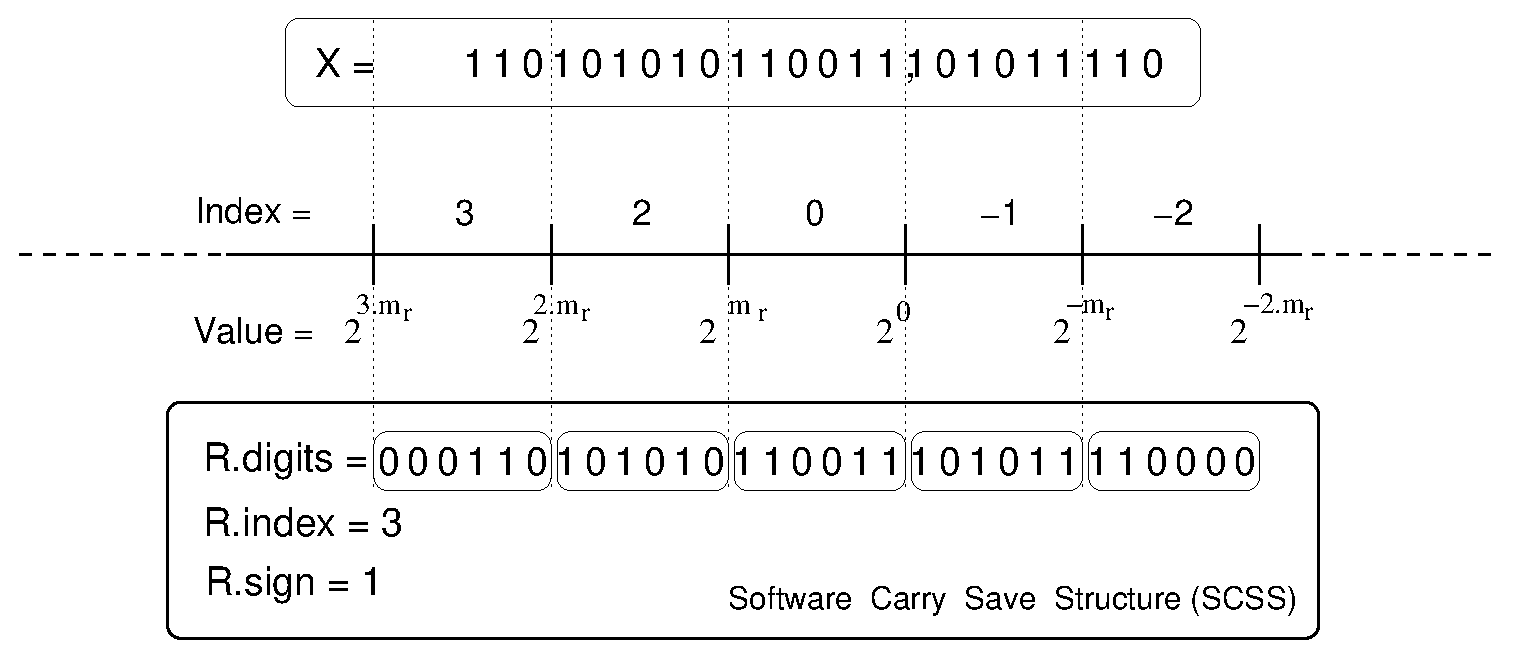
\includegraphics[width=0.7\textwidth]{fig_scs/exponent_representation} % image file name
\caption{The proposed format \label{fig:scsrepresentation}}
\end{center}
\end{figure}
  
In other words, the value  $x$ of a representation $R$  is:
\begin{equation}
\label{eqn4}
x = R.sign \times \sum_{j=1}^{n_r} R.digits[j] \times 2^{m_r * (R.index - j)}
\end{equation}

In such a \emph{normal} SCS number $R$, the bits from $m_I$ to $m_r$
of the $R.digits$ fields are thus set to zero. They will be exploited
by the algorithms to store temporary \emph{carry} information, and are
therefore called \emph{carry-save} bits. An SCS number where these
bits are non-zero is said to be non-normal.

The values of the parameters for use in \crlibm\ is $n_r=8$ digits of
$m_i=30$ bits stored on $m_r=32$-bit words. The worst-case precision
that this format may hold is when the most significant digit is equal
to $1$, meaning that an SCS numbers holds only $1+7\times 30=211$
significant digits.


\subsection{Arithmetic operations\label{sec:ops}}


\subsubsection{Conversion from double to SCS}
 A first method for converting a double precision floating
point number $d$ into an SCS representation is to extract the
exponent $d_{exp}$ from $d$, and then determine the corresponding
$R.index$ as the integer part of
$\frac{d_{exp}}{2^{m_r}}$.

Another method uses a variable number of multiplications by
$2^{m_r}$ or $2^{-m_r}$. This method is faster than the previous one
when the exponent of $d$ is close to $0$.

After testing both methods in \crlibm, the first method was preferred.


\subsubsection{Addition and subtraction}

The addition of two SCS numbers of the same sign consists in aligning,
then adding digits of the same order. Thanks to the carry-save bits,
all these additions will be \emph{exact} and \emph{independent}.
However the result will usually not be a normal SCS number: the sums
will have overflown in the carry-save bits. A \emph{renormalization}
procedure is presented in section \ref{renorm} to propagate these
carry bits and get again a normal SCS number.  However, the advantage
of SCS representation is that many SCS numbers can be summed before
needing to perform this expensive step (up to 7 with the choice of
parameters made in \crlibm).

The subtraction (addition of two numbers of opposite signs) is very
similar to the addition algorithm. It may also classically lead to a
cancellation, which may need an update of the index of the result.
However, as in other floating-point formats, a subtraction involving a
a cancellation is exact.

Although all the digit operations are exact, the addition or
subtraction of two numbers also classically involves a rounding error,
due to aligning the digits of same magnitude. For performance reason
this rounding is a truncation, so the worst-case relative error is one
ulp of the least accurate representable number, or $2^{-211}$.




%---------------- 
% MULTIPLICATION
%----------------
\subsubsection{Multiplication}

The multiplication of two normal SCS numbers involves the operations
depicted on the Figure \ref{fig:scsmultiplication}: The partial
products are computed (in parallel) and summed in columns. The
parameters are set up so that none of these operation overflow. Again,
the result is not a normal SCS number, and a renormalization procedure
(described below) has to be applied to empty the carry bits. However,
a few additions may follow a multiplication before this
renormalization, which allows for further optimization of algorithms
using SCS arithmetic. For instance, a polynomial evaluation can be
implemented with a renormalization after one multiplication and one
addition.

\begin{figure}[h]
\begin{center}
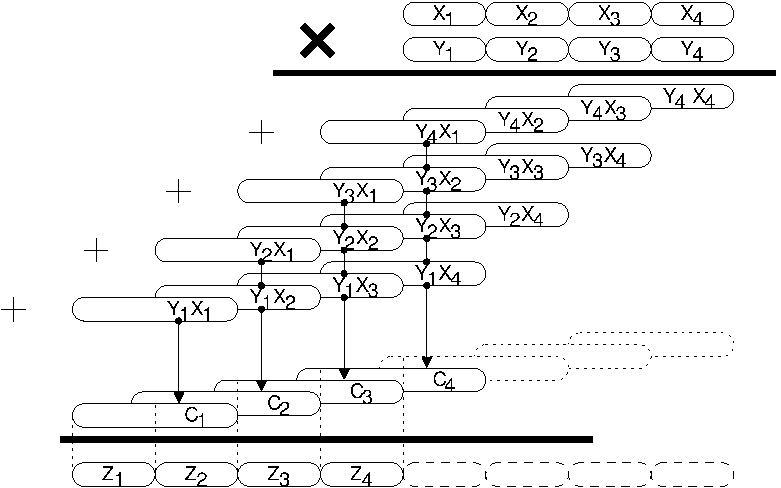
\includegraphics[width=0.7\textwidth]{fig_scs/multiplication}
\caption{SCS multiplication \label{fig:scsmultiplication}}
\end{center}
\end{figure}

Here also, a rounding error is involved when two $n_r$-digit numbers
are multiplied if the result is to fit on $n_r$ digits. The actual
implementation tests if the most significant digit ($z_1$ on
Figure~\ref{fig:scsmultiplication}) is null, in which case the index of
the result is that of $z_2$.

If the whole of the computations of
Figure~\ref{fig:scsmultiplication} are implemented, the worst case
for relative accuracy is again $2^{-211}$. However a further
optimization is to avoid computing the columns of lower magnitude, at
the expense of an increase in the rounding error. More specifically,
we compute 9 columns instead of 16.  The wors case is now when $z_1$
is null, in which case the relative error correspond to the truncation
of the 8 leftmost columns, whose maximum value is smaller than 3 ulps
of the SCS result. Therefore the relative error of the multiplication
is bounded by $2^{-208}$ with this optimization, which is still a
large overkill for the purpose of \crlibm.

This optimization is therefore implemented if the loop are hand-unrolled.
If they are not, the increased control complexity actually degrades
performance.


\subsubsection{Renormalization (carry propagation) \label{renorm}}

Renormalization is a carry propagation from the low order to high
order digits: Starting with an initially null carry, at each step, the
previous carry is added to the current digit, and this sum is then
split into two parts using masks. The low $m_r$ bits are a digit of
the normalized result, and the upper part is the next carry.

The actual algorithm is a little bit more complex. The initial
non-normal number may not be representable exactly as a normal SCS
number, therefore the index of the normalized result may have to be
increased by one or two.  Normalization thus again involves a rounding
error. Note that this error was already taken into account in the previous
discussions of addition and multiplication.




%-----------------
% CONVERSION BACK
%-----------------
\subsubsection{Conversion from SCS to floating-point}

A few (4 in the worst case) multiplications and additions suffice to
get the FP number closest to a SCS number.  For instance, for $m_I=53$
and $m_r=26$, we need to compute $d = A.sign \times 2^{A.index \times
  m_r} \times ( A.digits[0]+ 2^{-m_r} \times A.digits[1]+ 2^{-2.m_r}
\times A.digits[2]+ 2^{-3.m_r} \times A.digits[3])$. The number
$2^{A.index \times m_r}$ is build using integer masks. The actual
implementation of this formula is slightly less simple, but this
conversion is still very fast.


\subsubsection{Mixed 32- and 64-bit arithmetics}

An improvement implemented in \scslib\ was the combined use of integer 32- and 64-bit
arithmetics as follows: 

\begin{itemize}
\item MP digits are stored as 32-bit numbers where only a few bits are
  reserved for carries. This removes the main problem of the initial
implementation \cite{DefDin2002}, namely its memory inefficiency.

\item Addition uses 32-bit arithmetic. 

\item In the MP multiplication, the partial products are products of
  two 32-bit digits, which are 64-bit numbers. The column sums need
  thus to be computed using 64-bit arithmetic. This can be expressed
  in the C language in a non-ISO-C99, but de-facto standard way, as
  follows: 32-bit numbers have the \texttt{unsigned int} type; 64-bit
  numbers have the \texttt{unsigned long long int} type. When
  multiplying two digits, one is first cast into this 64-bit type.
  
  For UltraSPARC architectures (detected at build time) the
  conversion is to floating-point, but we will not detail this
  peculiarity further.
\end{itemize}


This works well because all modern processors either have 64-bit
integer units, or offer instructions which store the 64-bit product of
two 32-bit integers into two 32-bit registers. The compiler does the
rest well, because it is conceptually simple: casting unsigned 32-bit
into unsigned 64-bit is trivial; 64-bit addition is translated
straightforwardly into one 32-bit \emph{add} followed by one 32-bit
\emph{add-with carry}.




\subsubsection{Implementation considerations}

For portability purposes, the implemention uses C as defined by
the ISO C99 standard, and tries to use a recent version of \texttt{gcc}.
We could not exhibit a case where a native compiler from the processor
vendor (Intel or Sun) gave significantly better results than
\texttt{gcc}, which is probably a consequence of the simplicity of our
code.

However, when tuning for performance, we observed that the same code
which was efficient on one processor could lead to very poor results
on another.  Usually, this difference can be traced down to the
capabilities of the processor itself. The typical example is the
knowingly poor integer multiplication on UltraSPARC II. Sometimes
however, the processor should be able to perform well, and it is the
processor-specific backend of the compiler which is to blame, which
can be checked by observing the assembly code produced.  A typical
example is the casting of 32-bits digits to 64-bit arithmetic (or to
an FP number in the case of the UltraSPARC) in the multiplication
algorithm. In these cases we tried to change the programming style in
a way that works well on all processors. Sometimes it wasn't possible,
in which case the code contains, along with a generic version, several
processor-specific tricky versions of the problematic operation,
selected at compile time thanks to the GNU \texttt{automake/autoconf}
tools.


More surprisingly, we were disappointed by the higher-level
capabilities of the compilers, especially at unrolling loops. Our code
exhibits many small \texttt{for} loops whose size is known at
compile-time (usually $n$). This is the ideal situation for loop
unrolling, a technique well known and described in most textbooks on
compiler design. Options exist in most compilers to turn on this
optimisation. Unfortunately, leaving loop unrolling to the compiler
gives very poor results, even when compared to the non-unrolled case.
Since unrolling the loops by hand in the C code takes a few minutes,
we did it for the version of the library which we use ($m=30$, $n=8$).
It marginally increases the code sizes for this small $n$, and
sometimes provides a twofold improvement on speed, depending of the
processor. Of course, this is not satisfactory: We don't want to do it
for all values of $n$, nor do we want to study for each processor the
tradeoffs involved as $n$ increase. We expect however future compilers
to handle unrolling better, and we were surprised that no compiler had
a clear edge on the other in this respect. Some argue, however, that
this issue is pointless, as superscalarity, along with register
renaming and branch prediction inside modern processors, sum up to the
equivalent of dynamic unrolling of the code. In our tests (in 2003), it
doesn't: unrolling does bring a speed-up.








\section{Common Maple procedures \label{section:commonMaple}}


\subsection{Conversions}





Procedure \texttt{ieeedouble} returns the sign, the exponent and the
mantissa of the IEEE-754 double-precision number closest to input
value \texttt{x}.

\begin{lstlisting}[caption={ieeedouble},firstnumber=1]
ieeedouble:=proc(xx)
local x, sgn, logabsx, exponent, mantissa, infmantissa,powermin,powermax,expmin,expmax,expmiddle,powermiddle;
Digits := 100;
x := evalf(xx);
if (x=0) then sgn, exponent, mantissa := 1, -1022, 0
else
  if (x < 0) then sgn := -1
  else sgn := 1
  fi:
  x := abs(x);
  if x >=  2^(1023)*(2-2^(-53)) then mantissa := infinity; exponent := 1023
  else if x <= 2^(-1075) then mantissa := 0; exponent := -1022
      else
         if x <= 2^(-1022) then exponent := -1022
         else
# x is between 2^(-1022) and 2^(1024)
         powermin := 2^(-1022); expmin := -1022;
         powermax := 2^1024; expmax := 1024;
         while (expmax-expmin > 1) do
            expmiddle := round((expmax+expmin)/2);
            powermiddle := 2^expmiddle;
            if x >= powermiddle then
                powermin := powermiddle;
                expmin := expmiddle
            else
                powermax := powermiddle;
                expmax := expmiddle
            fi
          od;
# now, expmax - expmin = 1 and powermin <= x < powermax,
# powermin = 2^expmin and powermax = 2^expmax, so expmin is the exponent of x
         exponent := expmin;
         fi;
         infmantissa := x*2^(52-exponent);
	 if frac(infmantissa) <> 0.5 then mantissa := round(infmantissa)
            else
              mantissa := floor(infmantissa);
               if type(mantissa,odd) then mantissa := mantissa+1 fi
            fi;
         mantissa := mantissa*2^(-52);
      fi;
  fi;
fi;
sgn,exponent,mantissa;
end:
\end{lstlisting}


Procedure \texttt{ieeehexa} returns the hexadecimal representation of the nearest double to its input \texttt{x}.

\begin{lstlisting}[caption={ieeehexa},firstnumber=1]
ieeehexa:= proc(x)
local  hex2, xx, longint, expo, sgn, frac, resultat;
    if(x=0) then resultat:=["00000000","00000000"];
    elif(x=-0) then resultat:=["80000000","00000000"]; # nice try
    else
        xx:=ieeedouble(x);
        sgn:=xx[1]:
        expo:=xx[2]:
        frac:=xx[3]:
        if (expo = -1023) then
            longint := (frac)*2^51 ;   # subnormal
        else
            longint := (frac-1)*2^52 +   (expo+1023)*2^52;
        fi:
        if (sgn=-1) then
            longint := longint + 2^63;
        fi:
        longint := longint + 2^64:  # to get all the hexadecimal digits when we'll convert to string
        hex2:=convert(longint, hex);
        hex2:=convert(hex2, string):

        resultat:=[substring(hex2,2..9), substring(hex2,10..18)]:
    fi:
    resultat;
end proc:
\end{lstlisting}

Procedure \texttt{hexa2ieee} performs the reciprocal conversion.





Procedure \texttt{hi\_lo} returns two IEEE-double numbers $x\_hi$ and
$x\_lo$ so that $x = x\_hi + x\_lo + \epsilon_{-103}$.

\begin{lstlisting}[caption={hi\_lo},firstnumber=1]
hi_lo:= proc(x)
local x_hi, x_lo, res:
x_hi:= nearest(evalf(x)):
res:=x-x_hi:
if (res = 0) then
  x_lo:=0:
else
  x_lo:=nearest(evalf(res)):
end if;
x_hi,x_lo;
end:
\end{lstlisting}
\vspace{0.5cm}




Procedure \texttt{showHowDifficultToRound} takes a real number, and prints
the bits after the 53th of its nearest IEEE floating-point number.


\begin{lstlisting}[caption={showHowDifficultToRound},firstnumber=1]
showHowDifficultToRound:=proc(x)
local xb,xs,s,e,m:
    Digits:=200:
    s,e,m := ieeedouble(x):
    xb:=convert(evalf(x*2^(-e)),binary):
    xs:=convert(xb, string):
    substring(xs,55..153)
end proc:
\end{lstlisting}


\subsection{Procedures for polynomial approximation}


Procedure \texttt{Poly\_exact2} takes in arguments a polynomial
\texttt{P} and a integer \texttt{n}. It returns a truncated
polynomial, of which coefficients are exactly IEEE-double numbers. The
\texttt{n} first coefficients are written over 2 IEEE-double numbers.

\begin{lstlisting}[caption={poly\_exact2},firstnumber=1]
poly_exact2:=proc(P,n)
local deg,i, coef, coef_hi, coef_lo, Q:
Q:= 0:
convert(Q, polynom):
deg:=degree(P,x):
  for i from 0 to deg do
    coef :=coeff(P,x,i):
    coef_hi, coef_lo:=hi_lo(coef):
    Q:= Q + coef_hi*x^i:
    if(i<n) then
        Q := Q + coef_lo*x^i:
    fi:
  od:
  return(Q);
end:
\end{lstlisting}
\vspace{0.5cm}


We also have procedures for computing good truncated polynomial
approximation for a function. As they are useless to the proof, we do
not describe them here, the interested reader is referred to file
\texttt{maple/common-procedures.mpl} for more details.










\subsection{Accumulated rounding error in Horner evaluation
 \label{sec:Horner-maple}}



The following Maple procedures implement the error analysis described
in Section~\ref{sec:Horner}.

Procedure \texttt{compute\_abs\_rounding\_error} computes a bound on
the accumulated rounding error caused by the Horner evaluation of a
truncated polynomial. \texttt{poly} is the polynomial, \texttt{xmax} is the max value of
$|x|$, \texttt{nn} is the degree when \texttt{poly} is computed in double double, and the
first double-double operation is an addition.

This procedure returns the maximum absolute error, and safe bounds on the
minimum and maximum values of the function. It also checks on the fly
that the fast (test-free) versions of the double-double addition can
be used, and prints warnings if it not the case.

\begin{lstlisting}[caption={compute\_abs\_rounding\_error},firstnumber=1]
compute_abs_rounding_error:=proc(poly,xmax, nn)
local n, deg, delta, deltap, i, S, P, Snorm, Smin, Smax, prec:
deltap:=0:
delta:=0:
deg:=degree(poly):

prec:=53; # precision of the first iterations

S:=coeff(poly, x, deg):
Smax:=abs(S):
Smin:=Smax:

if nn<0 then n:=0: else n:=nn: fi:# sometimes called by compute_rel_rounding_error with n=-1

for i from (deg-1) to 0 by -1 do
  P:= convert(S*x, polynom):
  Smin := abs(coeff(poly,x,i)) - xmax*Smax : 
  if(Smin<=0) then 
    printf("Warning! in compute_abs_rounding_error, Smin<=0 at iteration %d, consider decreasing xmax\n",i);
  fi:
  delta:= evalf(xmax*deltap + 2**(-prec)*xmax*Smax):
  if i<n then 
    # fast Add22 ?    
    if abs(coeff(poly,x,i)) < xmax*Smax  # may be improved to xmax*Smax/2
    then printf("WARNING Add22 cannot be used at step %d, use Add22Cond\n" , i  );   
         printf("    coeff=%1.20e,  xmax*Smax=%1.20e"  ,  abs(coeff(poly,x,i)),  xmax*Smax );
    fi:
  fi:
  S:=convert(P+coeff(poly,x,i), polynom):
  Snorm:=evalf(infnorm(S, x=-xmax..xmax)):
  if i=n-1 then prec:=100: fi:  # from the addition of the n-1-th iteration
  deltap:= evalf(delta + 2**(-prec)*(delta + Snorm)): 
  Smax := Snorm + deltap:  
od:
deltap, Smin, Smax;
end proc:
\end{lstlisting}
\vspace{0.5cm}

Procedure \texttt{compute\_rel\_rounding\_error} computes a bound on
the total relative rounding error of a Horner polynomial evaluation,
in the same condition as the previous procedure.

\begin{lstlisting}[caption={compute\_abs\_rounding\_error},firstnumber=1]
compute_rel_rounding_error:=proc(poly,xmax, n)
local deg, p, rho, deltap, Smin, Smax:

deg:=degree(poly):
if(n>0) then p:=100: else p:=53: fi: 

if coeff(poly,x, 0) = 0 then
   deltap, Smin, Smax := compute_abs_rounding_error(poly/x,xmax, n-1):
   rho :=  (2^(-p)*(Smax+deltap) +deltap ) / Smin :
else
   deltap, Smin, Smax := compute_abs_rounding_error(poly,xmax, n):
   rho := deltap /  Smin:
fi:
rho;
end proc:
\end{lstlisting}
\vspace{0.5cm}

Procedures \texttt{compute\_abs\_rounding\_error\_firstmult} and
\texttt{compute\_abs\_rounding\_error\_firstmult} are similar to the
previous, but in the case when the first double-double operation is a
multiplication.



\subsection{Rounding}

Procedure \texttt{compute\_rn\_constant} computes a good constant for
the round-to-nearest test of Theorem~\ref{th:roundingRN1}. Its input
is a bound of the overall relative error of the approximation scheme.




\subsection{Using double-extended}

The file \texttt{maple/double-extended.mpl} contains procedures
similar to those previously described to handle double-extended
precision (64 bits of mantissa and 15 bits of exponent). This is
currently used in experimental code only: The \crlibm\ CVS repository
at \url{http://lipforge.ens-lyon.fr/} contains such code for
exponential and arctangent on Itanium, and arctangent on IA32
processors. For more details see \cite{DinDefLau2004LIP,DinErshGast2005}.




%%% Local Variables: 
%%% mode: latex
%%% TeX-master: "crlibm"
%%% End: 


 \chapter{The natural logarithm \label{chap:log}}
 This chapter is contributed by Florent de~Dinechin, with assistance from C. Daramy-Loirat and J.M. Muller. 

\newcommand{\middlei}{\mathrm{middle}[i]}


\section{Overview}

The worst-case accuracy required to compute a logarithm function
correctly rounded in double precision is $118$ bits according to
Lef�vre and Muller \cite{LefMul2004}.

We therefore proceed in two phases \cite{Ziv91}.  The first, quick
phase (program \texttt{log\_fast.c}) is accurate only to $57-64$ bits,
depending on the execution path as detailed below.  If this is not
enough to decide correct rounding, a second phase, accurate to $120$
bits using the SCS library is launched (program \texttt{log.c}).


\subsubsection*{Definition interval and exceptional cases}

The natural logarithm is defined over positive floating point numbers.  

\begin{itemize}
\item If $x \le 0$ , then $\log(x)$ should return $NaN$
\item If $x = +\infty$ , then $\log(x)$ should return $+\infty$. 
\end{itemize}

This is true in all rounding modes.

Concerning denormals, the smallest exponent of the logarithm of a
double-precision input number is $-53$ (for the input values
$\log(1+2^{-52})$ and $\log(1-2^{-52})$, as $\log(1+\epsilon) \approx
\epsilon$ when $\epsilon\rightarrow 0$). This will make it easy to
ensure that no denormal ever appears in the computation of the
logarithm of a double-precision input number.

\section{Quick phase}

\subsection{Overview of the algorithm}

The algorithm consists of an argument reduction using the well-known
property of the logarithm, and a polynomial evaluation using a degree
12 polynomial.


First we need to handle denormal inputs: If $x < 2^{-1022}$ , ie if x
is a subnormal number, then we use the equation
$$\log(x) = -52 * \log(2) + \log\left(\frac{x}{2^{-52}}\right)$$
where
$\displaystyle \frac{x}{2^{-52}}$ is now a normalized number.


Argument reduction starts with the decomposition of $x$ into its
mantissa $m$ and its exponent $E$. This decomposition can be computed
exactly. The mantissa is in $[1,2[$ and we prefer an interval centered
around $1$, so if needed the mantissa is  divided by 2 (and
the exponent incremented) to get
  
\begin{equation}
x = 2^{E}. y \label{eq:argred}
\end{equation}
where $E$ is an integer, and $y$ satisfies
\begin{equation}
\frac{11}{16}<\frac{\sqrt{2}}{2} < y < \sqrt{2}<\frac{23}{16} \quad.
\end{equation}

The final reconstruction will use the equation
 \begin{equation}
\log(x) = E \times \log(2) + \log(y) \quad.
\end{equation}


The interval $[\frac{11}{16},\frac{23}{16}]$ being too large for a
polynomial approximation of acceptable degree, it is broken down into
8 intervals given in Table~\ref{table:TablePolysLog1}.  Note that the
first four intervals are of size $2^{-4}$, while the last four are of
size $2^{-3}$.  The value of $i$, the index of the interval $X[i]$ to
which $y$ belongs, will be computed out of a few bits of $y$.

Noting $\middlei$ the middle of the $i$-th interval, the final range
reduction consists in computing $z = y - \middlei$. Again this range
reduction can be computed exactly thanks to Sterbenz lemma.  On each
interval, a polynomial $P[i](z)$ approximates $\log(y)$. In the
following $P[i]$ will be noted $P$ when no ambiguity arises.

Each polynomial has coefficients which are exactly representable as
IEEE doubles, with the two first coefficients being exactly
representable as the sum of two doubles: $c_0 = c_0^{hi} + c_0^{lo}$
and $c_1 = c_1^{hi} + c_1^{lo}$. Their relative approximation error is
also given in Table~\ref{table:TablePolysLog1}.


\begin{table}[htdp]\caption{The polynomials and their intervals \label{table:TablePolysLog1}}
\renewcommand{\arraystretch}{1.3}
\begin{center}
\begin{tabular}{|c|c|c|c|c|c|}
\hline
polynomial &    interval     &   $\middlei$   & $\max(|z|)$ & $\log_2(\maxrelerr{approx}[i])$\\
\hline  
P[0] & $[\frac{11}{16},\frac{12}{16}]$ &  $\frac{23}{32}$ & $2^{-5}$  &  63.24  \\ 
\hline                                                                                
P[1] & $[\frac{12}{16},\frac{13}{16}]$ &  $\frac{25}{32}$ & $2^{-5}$  &  62.23  \\
\hline                                                                                
P[2] & $[\frac{13}{16},\frac{14}{16}]$ &  $\frac{27}{32}$ & $2^{-5}$  &  61.19  \\ 
\hline                                                                                
P[3] & $[\frac{14}{16},\frac{15}{16}]$ &  $\frac{29}{32}$ & $2^{-5}$  &  60.09   \\ 
\hline                                                                                
P[4] & $[\frac{15}{16},\frac{17}{16}]$ &  $1$             & $2^{-4}$  &  61.72 \\ 
\hline                                                                                
P[5] & $[\frac{17}{16},\frac{19}{16}]$ &  $\frac{18}{16}$ & $2^{-4}$  &  59.33   \\ 
\hline                                                                                
P[6] & $[\frac{19}{16},\frac{21}{16}]$ &  $\frac{20}{16}$ & $2^{-4}$  &  62.34 \\ 
\hline                                                                                
P[7] & $[\frac{21}{16},\frac{23}{16}]$ &  $\frac{22}{16}$ & $2^{-4}$  &  63.03  \\ 
\hline
\end{tabular}\end{center}\end{table}



The polynomials  are evaluated thanks to a Horner scheme:

$$P(z) = c_0^{hi}+c_0^{lo} + z .(c_1^{hi} +c_1^{lo} + z .(c_2 + z
  .(c_3 + ...
 + z . (c_{11} + (c_{12} . z))))))))))))
$$
where the two last iterations may use double-double arithmetic if
required by the overall target accuracy, as detailed below.

Also note that the range of $z$ makes it easy to prove that no
denormal ever appear in the Horner evaluation of a polynomial. This
will be checked by the Maple procedure computing the rounding error of
the Horner scheme.


The reconstruction computes in double-double arithmetic: 
$$\log(x) \approx E\times \log(2) + P(z)$$
where $P(z)$ has been
computed by the previous step as the sum of two double-precision
numbers.  

The computation of $E\times \log(2)$ as a double-double exploits the
fact that $E$ is a small integer: The constant $\log(2)$ is stored as
the sum of two double-precision numbers
$l_h+l_l=\log(2)(1+\epsilon_{-101})$, with $l_h$ having the 11 lower
bits of its mantissa equal to zero, so that the computation of
$E\otimes l_h$ is exact. Now $E\times \log(2)$ may be computed as
Add12$(E\otimes l_h, E\otimes l_l)$.  There the Add12 procedure is
exact as well as the computation of $E\otimes l_h$, so the only errors
are the representation error in $l_l$ and the rounding error in
$E\otimes l_l$, the sum of which amounts to a total relative error
smaller than $\maxrelerr{reconstruction}=2^{-100}$ for the computation of $E\times \log(2)$.


\subsection{Error analysis}

Bounds on the polynomial approximation errors (both relative
$\maxrelerr{approx}[i]$ and absolute $\maxabserr{approx}[i]$) are easily computed under Maple
as infinite norms.

The rounding tests need a bound on the relative error, which can be computed as follows:

\begin{itemize}
\item If $E\ne0$, then the result is computed as $E\times \log(2) +
  P(z)$. We compute a bound on the relative error by dividing the sum
  of all absolute errors in the approximation scheme by the minimum
   value of the result:
  $$\maxrelerr{total} = \frac{\maxabserr{approx} +
    \maxabserr{rounding-poly} +
    \maxabserr{reconstruction}}{\min(|E\log(2)+P(x)|)}$$
  
  Here,
  $\maxabserr{reconstruction}=\max(E\log(2))\times\maxrelerr{reconstruction}$
  as computed previously, and $\maxabserr{approx}$ and
  $\maxabserr{rounding-poly}$ can be computed by generic Maple
  procedures of 
  \ref{section:commonMaple} for several variants of the polynomial evaluation which are
  detailed below.
  
  In this formula one sees several ways to handle the tradeoff between
  accuracy (which translates as percentage of cases where the slow,
  accurate phase will be needed) and performance of the quick phase:
\begin{itemize}
\item The absolute value of $P(z)$ is bounded by $0.37$. A bound on
  the denominator can therefore easily be deduced from the value of
  $|E|$.  In other terms, all things being equal, there will be less
  chances to go to the accurate phase for larger $E$.  It is therefore
  worth adding a test to the code which selects a rounding constant
  according to the value of $|E|$.
  
  The ``normal'' execution path of our algorithm performs the
  Horner polynomial evaluation with the three last operations (two additions
  and one multiplication) performed in double-double arithmetic. This
  leads to two values of $\maxrelerr{total}$: 
  \begin{itemize}
  \item {If $|E| \ge 24$} then we have  $\maxrelerr{total} = 2^{-64.8}$.
  \item {If $0<|E| < 24$} then we have $\maxrelerr{total} = 2^{-60.2}$.
  \end{itemize}
  
\item For even larger values of $|E|$, we can afford to have a large
  $\maxabserr{rounding-poly}$ and still get an acceptable
  $\maxrelerr{total}$. This allows us to evaluate the polynomial
  faster, without using double-double arithmetic. This situation will
  be referred to as the \emph{fast path} in the following. 
  
  Actually, performing only the last Horner addition in double-double
  on the fast path turns out to improve the average performance: It
  slows down the quick phase only a little, and greatly reduces
  $\maxabserr{rounding-poly}$, hence the chance of taking the slow,
  accurate phase. This in turn allows to take the fast path more
  often, \emph{i.e} for more values of $E$.
\end{itemize}

\item If $E=0$ then the reconstruction step is skipped, and the error
  $\maxrelerr{total}$ is given by the Maple procedures of
  \ref{section:commonMaple}. 
  
  It turns out that the polynomial $P[5]$ (the one which is centered
  on $1$ and has therefore a null coefficient of degree 0) leads to a
  relative rounding error which is much worse than that of the other
  polynomials. To still get an acceptable percentage of accurate phase
  in this case, and as the code contains a test if $E=0$ anyway, we
  chose to perform the polynomial evaluation in this case with one
  double-double multiplication more than in the normal case.

\end{itemize}


Actual values for this error analysis are summed up in
Table~\ref{tab:logerror}. In the implementation, we take as rounding
constant the worst case in each column. One remarks that the worst
case for the three first columns is for $P[5]$, which would suggest
yet another improvement: having specific rounding constants for $i=5$.
A closer look  at the average expected improvement shows that the
benefit will be minimal.


\begin{table}[!h]
  \begin{center}
    \begin{tabular}{|c|c||c|c|c|c|}
      \hline
      $P$ & $\infnorm{P}$ &  $E=0$ & $1 \le E < 24$ & $24\le E < 186$ & fast path\\ 
      \hline
P[1] & 0.375 & 61.44 & 60.43& 66.10  63.24\\ 
P[2] & 0.288 & 60.81 & 60.83& 66.16  63.29\\ 
P[3] & 0.208 & 60.02 & 61.11& 66.19  63.14\\ 
P[4] & 0.134 & 58.96 & 61.39& 66.27  63.34\\ 
P[5] & 0.065 & 57.63 & 60.04& 64.76  62.39\\ 
P[6] & 0.172 & 57.94 & 60.15& 65.13  63.01\\ 
P[7] & 0.272 & 59.89 & 60.23& 65.51  63.05\\ 
P[8] & 0.363 & 60.58 & 60.02& 65.65  63.23\\ 
      \hline
      \hline
    \end{tabular}
  \end{center}
  \caption{Error analysis for the various path in the algorithm. The table gives $-\log_2(\maxrelerr{total})$ in the different execution path.}
  \label{tab:logerror}
\end{table}

%%        P[1] & 0.375 & 61.10& 61.26 & 66.93 & 63.30\\ 
%%       \hline                             
%%       P[2] & 0.288 & 60.89& 61.87 & 67.20 & 63.46\\ 
%%       \hline                             
%%       P[3] & 0.208 & 60.47& 62.35 & 67.43 & 63.39\\ 
%%       \hline                             
%%       P[4] & 0.134 & 59.62& 62.77 & 67.65 & 63.73\\ 
%%       \hline                             
%%       P[5] & 0.065 & 57.68& 60.16 & 64.88 & 62.91\\ 
%%       \hline                             
%%       P[6] & 0.172 & 58.12& 61.22 & 66.20 & 62.78\\ 
%%       \hline                             
%%       P[7] & 0.272 & 59.93& 61.22 & 66.50 & 62.94\\ 
%%       \hline                             
%%       P[8] & 0.363 & 60.90& 61.19 & 66.81 & 63.23\\


\newpage
\subsection{Details of computer program}

A procedure \texttt{log\_quick} contains the computation shared by the
three functions \texttt{log\_rn}, \texttt{log\_ru} and
\texttt{log\_rd} (the function \texttt{log\_rz} calls either
\texttt{log\_ru} or \texttt{log\_rd}).  This procedures returns an
approximation to the log as two double-precision numbers, and an index
in an array of constants for testing if correct rounding is possible.
This array contains the relative error for directed rounding modes
(see~\ref{th:roundingDirected} p.~\pageref{th:roundingDirected}) , and
the rounding constant computed as per Theorem~\ref{th:roundingRN1}
p.~\pageref{th:roundingRN1} for round-to nearest.


\newpage
\subsubsection{Exceptional cases and argument reduction}

This part  is shown for \texttt{log\_rn}, but it is identical for the three functions.

\begin{lstlisting}[caption={Exceptional cases},firstnumber=1]
 double log_rn(double x) { 
   db_number y;
   double res_hi,res_lo,roundcst;
   int E,rndcstindex;

   E=0;
   y.d=x;

   /* Filter cases */
   if (y.i[HI_ENDIAN] < 0x00100000){        /* x < 2^(-1022)    */
     if (((y.i[HI_ENDIAN] & 0x7fffffff)|y.i[LO_ENDIAN])==0){
       return -1.0/0.0;     
     }                                     /* log(+/-0) = -Inf */
     if (y.i[HI_ENDIAN] < 0){ 
       return (x-x)/0;                      /* log(-x) = Nan    */
     }
     /* Subnormal number */
     E = -52;           
     y.d *= two52.d;      /* make x a normal number    */ 
   }
    
   if (y.i[HI_ENDIAN] >= 0x7ff00000){
     return  x+x;                                /* Inf or Nan       */
   }
   
   /* reduce to  y.d such that sqrt(2)/2 < y.d < sqrt(2) */
   E += (y.i[HI_ENDIAN]>>20)-1023;                              /* extract the exponent */
   y.i[HI_ENDIAN] =  (y.i[HI_ENDIAN] & 0x000fffff) | 0x3ff00000;        /* do exponent = 0 */
   if (y.d > SQRT_2){
     y.d *= 0.5;
     E++;
   }

   /* Call the actual computation */
   log_quick(&res_hi, &res_lo, &rndcstindex, &y, E);
\end{lstlisting}


\begin{tabular}{ll}
Lines  6,7 &  Initialize E and y\\
Line 10 & Test if x is null, negative or a subnormal number.\\
Line 11,12 & Test if x is $\pm 0$ and return  $-\infty$ \\
Line 14,15 & If x is negative,  return NaN and raise an exception.\\
Line 18,19 & else $x$ is subnormal, then compute:\\
& $log(x) = -52\times log(2) + log(\frac{x}{2^{-52}})$ \\
& (this computation is exact) \\ 
Line 22,23 & If $x$ is $\infty$ or NaN, return $\infty$ or NaN.\\
Line 27 & E contains x 's exponent. \\
Line 28 & y.d is reduced to $\frac{x}{2^E}$. Correct because $y$ was a normal number.\\
Line 29-31 & Now, we have: $ 1 \leq y.d < 2$ and we want $ \frac{1}{\sqrt2} \leq y.d < \sqrt2$.\\
& So, if it's not the case, we update E and y.\\
\end{tabular}


\newpage

\begin{lstlisting}[caption={Procedure \texttt{log\_quick}},firstnumber=1]
static void log_quick(double *pres_hi, double *pres_lo, int* prndcstindex, db_number * py, int E) {
   double ln2_times_E_HI, ln2_times_E_LO, res_hi, res_lo;
   double z, res, P_hi, P_lo;
   int k, i;
   
    /* find the interval including y.d */
    i = ((((*py).i[HI_ENDIAN] & 0x001F0000)>>16)-6) ;
    if (i < 10)
      i = i>>1;
    else
      i = ((i-1)>>1);
    
    z = (*py).d - (middle[i]).d;  /* (exact thanks to Sterbenz Lemma) */
    

    /* Compute ln2_times_E = E*log(2)   in double-double */
    Add12( ln2_times_E_HI, ln2_times_E_LO, ((double)E)*ln2hi.d, ((double)E)*ln2lo.d); 


    /* Now begin the polynomial evaluation of log(1 + z)      */

    res = (Poly_h[i][DEGREE]).d;

    for(k=DEGREE-1; k>1; k--){
      res *= z;
      res += (Poly_h[i][k]).d;
    }

    if((ln2_times_E_HI*ln2_times_E_HI < MIN_FASTPATH*MIN_FASTPATH)) {
      /* Slow path */
      if(E==0) {
        *prndcstindex = 0 ;
        /* In this case we start with a double-double multiplication to get enough relative accuracy */ 
        Mul12(&P_hi, &P_lo, res, z); 
        Add22(&res_hi, &res_lo, (Poly_h[i][1]).d,  (Poly_l[i][1]).d, P_hi, P_lo);
        Mul22(&P_hi, &P_lo, res_hi, res_lo, z, 0.); 
        Add22(pres_hi, pres_lo, (Poly_h[i][0]).d, (Poly_l[i][0]).d, P_hi, P_lo);
      } 
      else
        {
          if((ln2_times_E_HI*ln2_times_E_HI > 16.5*16.5))
            *prndcstindex = 2; 
          else 
            *prndcstindex =1;
          P_hi=res*z;  P_lo=0.; 
          Add22(&res_hi, &res_lo, (Poly_h[i][1]).d,  (Poly_l[i][1]).d, P_hi, P_lo);
          Mul22(&P_hi, &P_lo, res_hi, res_lo, z, 0.); 
          Add22(&res_hi, &res_lo, (Poly_h[i][0]).d, (Poly_l[i][0]).d, P_hi, P_lo);
      
        /* Add E*log(2)  */
          Add22(pres_hi, pres_lo, ln2_times_E_HI, ln2_times_E_LO, res_hi, res_lo);
        }
    }
    else { /* Fast path */
      
      *prndcstindex = 3 ;
      res =   z*((Poly_h[i][1]).d + z*res);
      Add22(&res_hi, &res_lo, (Poly_h[i][0]).d , (Poly_l[i][0]).d, res, 0.);

        /* Add E*log(2)  */
      Add22(pres_hi, pres_lo, ln2_times_E_HI, ln2_times_E_LO, res_hi, res_lo);
    }
}
\end{lstlisting}

\begin{tabular}{ll}
Line 7  & To find the interval $X_i$ containing $y$, we  look upon\\ 
        &   the last bit of the exponent and the 4 first bits of the mantissa.\\
Lines 8-11  & Reduction over $i$ in order to have an index $i$ between 0 and 7\\
        & corresponding to the 8 intervals of Table~\ref{table:TablePolysLog1}.\\
Line 13 & Let us prove that z.d is computed exactly, without rounding error: \\
& \vspace{1ex}To use Sterbenz Lemma, we need to prove that  ${\middlei}/{2} <  y.d < \middlei \times 2$.\\ 
& \vspace{1ex}For every i in $[0;7]$, we have $\middlei-\frac{1}{16} \leq y.d \leq \middlei+\frac{1}{16}$.\\
& \vspace{1ex}Table~\ref{table:TablePolysLog1} gives: $\frac{25}{32} \leq {\middlei} \leq \frac{22}{16}$\\ 
& \vspace{1ex}Therefore ${\middlei}/{2} \leq \frac{22}{32} < \frac{23}{32} \leq \middlei - \frac{1}{16} \leq y.d$\\
& and $y.d \leq \middlei + \frac{1}{16} \leq \frac{23}{16} < \frac{25}{16} \leq \middlei\times 2$\\
Line 17 & The computation of $E\log(2)$ is done as early as possible. \\
        & As stated previously, the relative error here is smaller than $2^{-100}$\\
Lines 22-27 & Begin of Horner evaluation in double arithmetic\\
Line 29 & This test is equivalent to $|ln2\_times\_E_HI| < \mathtt{MIN\_FASTPATH}$.\\
        & As $|E|$ is an integer smaller than $2048$, neither overflow nor denormal can occur.\\
        & Currently $\mathtt{MIN\_FASTPATH}=128.5$ but the Maple programs in \texttt{coef\_log.mw}\\
        & allow to change this value.\\
Lines 31-53 & Slow path, divided two cases:\\
Lines 31-38 & ~Case $E=0$: in this case, there is no addition of $E\log(2)$ in the end, \\
            & ~~~to reach the required relative accuracy we do two $\times$ and two $+$ in double double\\
Lines 40-52 & ~Case $E\ne 0$ Thanks to the final addition to $E\log(2)$,\\
            & ~~we have to bound only the absolute accuracy of the polynomial evaluation\\
            & ~~which allows to save the first Mult22.\\
Lines 54-62 & Fast path : the polynomial evaluation is entirely in double-precision, and the \\
            & ~ final addition with a large  $E\log(2)$ scales the resulting bad absolute accuracy\\
            & ~ to acceptable relative accuracy\\ 
Lines 34,36,47 & None of the intermediate values reaches  $2^{970}$ so we may use the unconditional Mul22.\\
Lines 35,37,46,48 & The Maple procedure checks that the first argument is always greater \\
                  & than the second, so we may use the unconditional Add22.\\
Lines 51,61 & $E\log(2)$ is greater than  $\log(2)\approx 0.69$, and $\infnorm{P_i(x)}<0.4$\\
                  & so we may use the unconditional Add22.\\

\end{tabular}



\subsection{Rounding}

\subsubsection{Rounding to the nearest}

The code for rounding is strictly identical to that of
Theorem~\ref{th:roundingRN1}.  The condition to this theorem that
$\mathtt{res\_hi}\ge 2^{-1022+53}$ is ensured by the image domain of
the $\log$ over the floating-point numbers: as already mentionned, the
smallest possible value of the logarithm of a floating-point number is
larger than $2^{-53}$. As $\mathtt{res\_hi}$ approximates this value
with a relative accuracy much smaller than $1$, the condition is
ensured.


\subsection{Directed rounding}

Here again, the code is strictly identical to that of
Theorem~\ref{th:roundingDirected}, and the conditions to this theorem
are ensured by the image domain of the log.




%%%%%%%%%%%%%%%%%%%%%%%%%%%%%%%%%%%%%%%%%%%%%%%%%%%%%%%%%%%%%%%%%%%%%%%%%%%%%%%%%%%%%
\section{Accurate phase}


There is only one accurate function, called is \texttt{scs\_log}. It
returns an SCS number, which is rounded in the required mode by one of
\texttt{scs\_get\_d}, \texttt{scs\_get\_d\_pinf} and
\texttt{scs\_get\_d\_minf} in the corresponding functions in
\texttt{log\_fast.c}.


\subsection{Argument reduction}

The first argument reduction is the same as in the quick phase.
Therefore the function  \texttt{scs\_log}  take as arguments $y$ and $E$, computed
in the quick phase (similarly, exceptional cases are not considered
again).

As in the quick phase, we will compute the log using $$\log(x) = E \times log(2) + log(1+f)\quad .$$

Now we define $w_i = 1 + i\times2^{-4}$, for $i = -6 ... 6$, and we select the $w_i$ closest to $1+f$, in order to have: 

$$log(1+f) = log(w_i) + log(1+\frac{1+f-w_i}{w_i})$$

where $r=\frac{1+f-w_i}{w_i} \leq 2^{-5}$.

The values of $log(w_i)$, $1/w_i$ and $log(2)$ are tabulated. We
therefore compute the reduced argument $R = (1+f-w_i)/w_i$ by a
subtraction in double precision (exact thanks to Sterbenz Lemma)
followed by a conversion to SCS (also exact) and an SCS multiplication
(relative error smaller than $2^{-207}$ including the error in tabulating $1/w_i$).

\begin{lstlisting}[caption={Argument reduction},firstnumber=1]
void scs_log(scs_ptr res, db_number y, int E){ 
  scs_t R, sc_ln2_times_E, res1, addi;
  scs_ptr ti, inv_wi;
  db_number z, wi;
  int i;

 /* to normalize y.d and round to nearest      */
  /* + (1-trunc(sqrt(2.)/2 * 2^(4))*2^(-4) )+2.^(-(4+1))*/ 
  z.d = y.d + norm_number.d; 
  i = (z.i[HI_ENDIAN] & 0x000fffff);
  i = i >> 16; /* 0<= i <=11 */
  

  wi.d = ((double)(11+i))*0.0625;

  /* (1+f-w_i) */
  y.d -= wi.d; 
  
  /* Table reduction */
  ti     = table_ti_ptr[i]; 
  inv_wi = table_inv_wi_ptr[i];
   
  /* R = (1+f-w_i)/w_i */
  scs_set_d(R, y.d);
  scs_mul(R, R, inv_wi);

\end{lstlisting}




\subsection{Polynomial approximation}

$log(1+\frac{1+f-w_i}{w_i})$ is approximated by a polynomial
$Q(\frac{1+f-w_i}{w_i})$ with an overall relative error less than $2^{-130}$.

The polynomials are available in \texttt{log.h}.


\begin{lstlisting}[caption={Polynomial approximation},firstnumber=1]
  scs_mul(res1, constant_poly_ptr[0], R);
  for(i=1; i<20; i++){
    scs_add(addi, constant_poly_ptr[i], res1);
    scs_mul(res1, addi, R);
  }
\end{lstlisting}

TODO:
Add a Maple script that computes the relative error of a polynomial given an error on the input. It is required here.




\subsection{Reconstruction}
At the end, we compute:

\begin{equation}result = E\times log(2) + log(w_i) + Q(\frac{1+f-w_i}{w_i})\end{equation}

\begin{lstlisting}[caption={Reconstruction},firstnumber=1]
  if(E==0){
    scs_add(res, res1, ti);
  }else{
    /* sc_ln2_times_E = E*log(2)  */
    scs_set(sc_ln2_times_E, sc_ln2_ptr);

    if (E >= 0){
      scs_mul_ui(sc_ln2_times_E, (unsigned int) E);
    }else{
      scs_mul_ui(sc_ln2_times_E, (unsigned int) -E);
      sc_ln2_times_E->sign = -1;
    }
    scs_add(addi, res1, ti);
    scs_add(res, addi, sc_ln2_times_E); 
  }
}
\end{lstlisting}



\subsection{Rounding}

As already stated, the procedure \texttt{scs\_log} returns an SCS number which is rounded
in the required mode by the caller function. 



%%%%%%%%%%%%%%%%%%%%%%%%%%%%%%%%%%%%%%%%%%%%%%%%%%%%%%%%%%%%%
\section{Analysis of the logarithm performance}
\label{section:log_results}
The input numbers for the performance tests given here are random
positive double-precision numbers with a normal distribution on the
exponents. More precisely, we take random 63-bit integers and cast
them into double-precision numbers.  


In average, the second step is taken in 0.23\% of the calls, which
seems a rather good balance considering the respective costs of the
first and second steps (seen in the table as the min and max times,
respectively).


\subsection{Speed}
Table \ref{tbl:log_abstime} (produced by the \texttt{crlibm\_testperf}
executable) gives absolute timings for a variety of processors and
operating systems.  

\begin{table}[!htb]
\begin{center}
\renewcommand{\arraystretch}{1.2}
\begin{tabular}{|l|r|r|r|}
\hline
 \multicolumn{4}{|c|}{Pentium 4 Xeon / Linux Debian sarge / gcc 3.3}   \\ 
 \hline
                         & min time      & max time      & avg time \\ 
 \hline
 \hline
 \texttt{libm}           & 180          & 6612          &        189 \\ 
 \hline
  \texttt{mpfr}          & 4            & 331372        &      61529 \\ 
 \hline
  \texttt{libultim}      & 240          & 370036        &        520 \\ 
 \hline
 \texttt{crlibm}         & 336          & 53700         &        529 \\ 
 \hline
 \hline
  \multicolumn{4}{|c|}{PowerPC G4 / MacOS X / gcc2.95}   \\
 \hline
                         & min time      & max time      & avg time \\
 \hline
 \texttt{libm}           & 14           & 16            &         15 \\
 \hline
  \texttt{mpfr}          & 4610         & 8620          &       4895 \\
 \hline
  \texttt{libultim}      & 20           & 19890         &         22 \\
 \hline
 \texttt{crlibm} (without FMA)      & 5            & 1241          &         32 \\
\hline
 \texttt{crlibm} (using FMA)        & 5           & 1144          &         24 \\

\hline
\end{tabular}
\end{center}
\caption{Absolute timings for the logarithm (arbitrary units)
  \label{tbl:log_abstime}}
\end{table}

Contributions to this table for new processors/OS/compiler combinations are welcome.



\subsection{Memory requirements}

Table size is
\begin{itemize}
\item for the \quick\ phase,
  $8\times 15\times8=960$ bytes for the eight polynomials, plus
  another $64$ bytes for the rounding constants, or a total of exactly
  1kB.
\item for the \accurate\ phase, $1+13+13+20$ SCS constants:  $\log(2)$,
  the 13 $log(w_i)$ and the 13 $\frac{1}{w_i}$,  the polynomial of
  degree 20 with a null first coefficient. This amounts to a little more than 2kB.
\end{itemize}





%%%%%%%%%%%%%%%%%%%%%%%%%%%%%%%%%%%%%%%%%%%%%%%%%%%%%%%%%%%%%
\section{Conclusion and perspectives}


In the log we have a fairly good balance between both evaluation
phases, which was obtained thanks to automated testing of various
sceniarii. The main lesson learned here was that designing a rigorous
proof along with the code helped tuning performance, by helping
managing the tradeoff between speed and accuracy of the first path.

Our log is a few percent slower in average than Ziv/IBM's, but if we
inline the code of \texttt{log\_quick} then it becomes faster than
Ziv's: Inlining saves a function call, but also allows other minor
improvements, like removing the need for the constant index, and
loading the constants for the rounding test in advance to hide their loading
time. However, as it increases the size of the code and degrades its
maintainability, we believe the current approach makes more sense in
\crlibm.

It might be interesting for some applications to add a fast execution
paths for values around $1$, as Ziv does: This is the situation
where our quick phase is slowest and our second phase most often
taken. However it will not show any improvement in our test protocol.
Besides, it is probably more important to implement the standard $\log(1+x)$
function, which is designed specifically for this case.

Finally, we did not try to implement the argument reduction used in
the accurate phase for the quick phase, mostly because it is not
exact (contrary to the one we used), which complicates error analysis. This is, however, another
obvious path to explore.


 \chapter{The exponential \label{chap:exp}}
 This chapter is contributed by David Defour, with assistance from F.
de~Dinechin and J.M. Muller.

Warning: THIS CHAPTER IS OBSOLETE. As of version 0.10beta there is a
triple-double implementation of the exponential which is more
efficient than the one presented here. The proof will be written before 0.10 comes out of beta.


This chapter was the first to be written, while the library
was in prototype stage. It may therefore present some inconsistencies
in notations with the other chapters. 


\section{Overview of the algorithm}
\label{section:overview}
We are now going to present and proof the correct rounding of the evaluation scheme chosen for the exponential within \emph{crlibm}.

We have done the evaluation of the exponential in two steps. First, we use the \emph{quick} phase of the algorithm to get an approximation good to $68$ bits of the result. Then we perform a test to check whether we need to use the \emph{accurate} phase, based on multiprecision operators from SCSlib~\cite{SCSweb} .

To increase the trust of the code, with have included constants in hexadecimal format, and for concision reason only the one in big endian format are present. However to help the reader we are giving the corresponding decimal values.

\section{Quick phase}

Here is the general scheme chosen for the first step of the evaluation of the exponential : 

\begin{enumerate}
\item 
{\bf ``Mathematical'' range reduction} \\
We want to compute $\exp(x)$. We evaluate the reduced argument $$(r\_hi + r\_lo)\in [-\ln(2)/2, +\ln(2)/2]$$ such that :

$$x=k. \ln(2) + (r\_hi + r\_lo)$$

then $\exp(x) = \exp(r\_hi + r\_lo) . 2^{k}$ with $(r\_hi + r\_lo) \in [-\ln(2)/2, +\ln(2)/2]$
\item
{\bf Tabular range reduction} \\

Let $index\_flt$ be the first 8 bits of $(r\_hi + r\_lo)$, we want

$$\exp(r\_hi + r\_lo) = \exp(index\_flt) \times \exp(rp\_hi + rp\_lo)$$

where $(rp\_hi + rp\_lo) = (r\_hi + r\_lo) - index\_flt$ such that $(rp\_hi + rp\_lo) \in [-2^{-9}, +2^{9}]$ and $\exp(index\_flt)=(ex\_hi + ex\_lo)$ is obtain with a table lookup.


\item
{\bf Polynomial evaluation} \\
We evaluate the polynom $P\_r$ of degree 3 such that : 

$$exp(rp\_hi + rp\_lo) \approx 1 + (rp\_hi + rp\_lo) + \frac{1}{2}.(rp\_hi+rp\_lo)^2 +(rp\_hi+rp\_lo)^3 . (P\_r)$$

with
$P\_r = c_0 + c_1 .rp\_hi + c_2 .rp\_hi^2 + c_3 .rp\_hi^3$
and
$rp\_hi \in [-2^{-9}, +2^{9}]$

\item
{\bf Reconstruction} \\

$$
\begin{array}{rcl}
\exp(x) &=& 2^k . (ex\_hi+ex\_lo). \\
 &&(1 + (rp\_hi+rp\_lo) + \frac{1}{2}.(rp\_hi+rp\_lo)^2 + (rp\_hi+rp\_lo)^3.P\_r)
. (1+\epsilon_{-68})\\
\end{array}
$$

\end{enumerate}




\subsection{Handling special cases}

\subsubsection{Select the evaluation range to avoid overflows and underflows}
\label{chap3:exp:overflows}
In the sequel of this paper, we will consider input numbers in the range $[u\_bound, o\_bound]$, where $u\_bound$ and $o\_bound$ are :


$$u\_bound = \bigtriangleup \left(\ln\left(\left(1-2^{-53}\right).2^{-1075}\right)\right) = -745.1332\ldots$$
$$o\_bound = \bigtriangledown \left( \ln \left(\left(1-2^{-53}\right).2^{1024}\right)\right) = 709.7827\ldots$$

In the rounding mode to nearest, the exponential of a number greater than $o\_bound$ is an overflow, whereas the exponential of a number less than $u\_bound$ is rounded to $0$, and raise an inexact flag.

However, subtler under/overflow situations may arise in two cases, which we should avoid :
\begin{itemize}
\item An intermediate computation may raise an overflow although the final result is representable as an IEEE-754 floating-point number.

\item In IEEE-754 arithmetic, when a result is between $2^{-1023}$ and $2^{-1074}$, a gradual underflow exception arises to signal that the precision of the result is reduced in a drastic way.
\end{itemize}

In both cases, as we will show in the following, it is possible to avoid the exception by predicting that it will occur, and appropriately scaling the input number in the range reduction phase.



\subsubsection{Rounding to nearest}

\begin{lstlisting}[caption={Handling special cases in rounding to nearest},firstnumber=1]
static const union{int i[2]; double d;}
#ifdef BIG_ENDIAN
 _largest    = {0x7fefffff, 0xffffffff},
 _smallest   = {0x00000000, 0x00000001},
 _u_bound    = {0xC0874910, 0xD52D3052}, /* -7.45133219101941222107e+02 */
 _o_bound    = {0x40862E42, 0xFEFA39F0}; /*  7.09782712893384086783e+02 */
#else
 ...
#endif
#define largest    _largest.d
#define smallest   _smallest.d
#define u_bound    _u_bound.d
#define o_bound    _o_bound.d

unsigned int hx;

hx  = HI(x);                                         (*@ \label{exp:code:1} @*)
hx &= 0x7fffffff;                                    (*@ \label{exp:code:3} @*)

/* Filter special cases */
if (hx >= 0x40862E42){                               (*@ \label{exp:code:4} @*)
  if (hx >= 0x7ff00000){                             (*@ \label{exp:code:5} @*)
    if (((hx&0x000fffff)|LO(x))!=0)                  (*@ \label{exp:code:6} @*)
      return x+x;                            /* NaN */  (*@ \label{exp:code:7} @*)
    else return ((hx&0x80000000)==0)? x:0.0; /* exp(+/-inf) = inf,0 */(*@ \label{exp:code:8} @*)
  }
  if (x > o_bound) return largest *largest ; /* overflow  */  (*@ \label{exp:code:9} @*)
  if (x < u_bound) return smallest*smallest; /* underflow */  (*@ \label{exp:code:10} @*)
}


if (hx <= 0x3C900000) return 1.;             /* if (hx <= 2^(-54)) */ (*@ \label{exp:code:10bis} @*)

\end{lstlisting}


\begin{preuve}
\begin{longtable}[c]{@{line }p{0.08\textwidth}p{0.81\textwidth}}
% en cas de cesure c'est ce que l'on place 
% en debut de page
\endhead
% en fin de page
\endfoot 
% en fin de derniere page
\endlastfoot 
\ref{exp:code:1} & Put the high part of $x$ in $hx$.
\\
\ref{exp:code:3} & Remove the sign information within $hx$. It will make tests on special cases simpler.
\\
\ref{exp:code:4} & Test equivalent to $if (|x|>=709.7822265625)$. This test is true if $x>u\_bound$, $x<o\_bound$, $x=\pm inf$ or $x=NaN$. This test is performed with integers to make it faster.
\\
(\ref{exp:code:5}-\ref{exp:code:7}) & Test if $x=\pm inf$ or $x=NaN$ and give the corresponding results (exact $+\infty$ or $0$).
\\
\ref{exp:code:9} & Under the assumption that the compiler correctly translates the floating-point number we have $o\_bound = 390207173010335/549755813888$. If $x>o\_bound$ then $\exp(x)=+\inf$. The multiplication $largest*largest$ leaves to the compiler the generation of an overflow and the corresponding flags. 
\\
\ref{exp:code:10} & Under the assumption that the compiler correctly translates the floating-point number we have $u\_bound = -3277130554578985/4398046511104$. If $x<u\_bound$ then $\exp(x)=+0$.  The multiplication $largest*largest$ leaves to the compiler the generation of an underflow and the corresponding flags.
\\
\ref{exp:code:10bis} & Test equivalent to $if (|x| \leq 2^{-54})$. This test is performed with integers to make it faster and is valid because $x \notin \{NaN, \infty\}$. In addition, this test allows to handle cases when $x$ is a subnormal number. We have the following property : 
\begin{prop}
  \label{chap3:exp:prop10bis}
  $|x| > 2^{-54}$~~and~~~~$x\notin\{NaN, \infty\}$
\end{prop}
Indeed, in rounding to nearest, if $|x| \leq 2^{-54}$ then $\exp(x) = 1.0$. This test prevents to encounter a subnormal number in the rest of the program.

\\
\end{longtable}
\end{preuve}




\subsubsection{Rounding toward $+ \infty$}

\begin{lstlisting}[caption={Handling special cases in rounding toward $+\infty$},firstnumber=1]
static const union{int i[2]; double d;}
#ifdef BIG_ENDIAN
 _largest    = {0x7fefffff, 0xffffffff},
 _smallest   = {0x00000000, 0x00000001},
 _u_bound    = {0xC0874910, 0xD52D3052}, /* -7.45133219101941222107e+02 */
 _o_bound    = {0x40862E42, 0xFEFA39F0}, /*  7.09782712893384086783e+02 */
 _two_m52_56 = {0x3CB10000, 0x00000000}; /*  2.35922392732845764840e-16 */
#else
 ...
#endif
#define largest    _largest.d
#define smallest   _smallest.d
#define u_bound    _u_bound.d
#define o_bound    _o_bound.d
#define two_m52_56 _two_m52_56.d


unsigned int hx;

hx  = HI(x);    
hx &= 0x7fffffff;

/* Filter special cases */
if (hx >= 0x40862E42){
  if (hx >= 0x7ff00000){
    if (((hx&0x000fffff)|LO(x))!=0)
      return x+x;                            /* NaN */
    else return ((hx&0x80000000)==0)? x:0.0; /* exp(+/-inf) = inf,0 */
  }
  if (x > o_bound) return largest*largest;   /* overflow  */
  if (x < u_bound) return smallest*1.0;      /* 2^(-1074) */
}

if (hx < 0x3CA00000){                        /* if (hx <= 2^(-53)) */
  if (HI(x) < 0)
    return 1. + smallest;                    /* 1 and inexact */
  else
    return 1. + two_m52_56;                  /* 1 + 2^(-52) and inexact */ 
}

\end{lstlisting}


\begin{preuve}
This program is similar to the one used in rounding to nearest mode with the exception of :
\begin{itemize}
\item
When $(x < u\_bound)$, in rounding toward $+\infty$, we have to give as result the smallest representable number ($2^{-1074}$) with the inexact flag raised.
\item
When $(|x| < 2^{-53})$, in rounding toward $+\infty$, we have to give as result $1.0$ if $x<0$ with the inexact flag raised or $1+2^{-52}$ with the inexact flag raised if $x>0$.
\end{itemize}
\end{preuve}



\subsubsection{Rounding toward $- \infty$}

\begin{lstlisting}[caption={Handling special cases in rounding toward $- \infty$},firstnumber=1]
static const union{int i[2]; double d;}
#ifdef BIG_ENDIAN
 _largest    = {0x7fefffff, 0xffffffff},
 _smallest   = {0x00000000, 0x00000001},
 _u_bound    = {0xC0874910, 0xD52D3052}, /* -7.45133219101941222107e+02 */
 _o_bound    = {0x40862E42, 0xFEFA39F0}, /*  7.09782712893384086783e+02 */
 _two_m52_56 = {0x3CB10000, 0x00000000}; /*  2.35922392732845764840e-16 */
#else
 ...
#endif
#define largest    _largest.d
#define smallest   _smallest.d
#define u_bound    _u_bound.d
#define o_bound    _o_bound.d
#define two_m52_56 _two_m52_56.d

unsigned int hx;

hx  = HI(x);
hx &= 0x7fffffff;

/* Filter special cases */
if (hx >= 0x40862E42){
  if (hx >= 0x7ff00000){
    if (((hx&0x000fffff)|LO(x))!=0)
      return x+x;                            /* NaN */
    else return ((hx&0x80000000)==0)? x:0.0; /* exp(+/-inf) = inf,0 */
  }
  if (x > o_bound) return largest*1.0;       /* (1-2^(-53))*2^1024  */ 
  if (x < u_bound) return smallest*smallest; /* underflow */
}

if (hx < 0x3CA00000){                        /* if (hx <= 2^(-53))   */
  if (HI(x) < 0)
    return 1. - two_m52_56;                  /* 1-2^(-52) and inexact */
  else
    return 1. + smallest;                    /* 1 and inexact */
}

\end{lstlisting}



\begin{preuve}
This program is similar to the one used in rounding to nearest mode with the exception of :
\begin{itemize}
\item
When  $(x > o\_bound)$, in rounding toward $-\infty$, we have to give as result the largest representable number  ($(1-2^{-53}).2^{1024}$) with the inexact flag raised.
\item
When $(|x| < 2^{-53})$, in rounding toward $-\infty$, we have to give as result  $1.0 - 2^{-52}$ if $x<0$ with the inexact flag raised or $1.0$ with the inexact flag raised if $x>0$.
\end{itemize}
\end{preuve}



\subsubsection{Rounding toward $0$}

The exponential function is continue and positive, therefore the rounding toward $0$ mode is equivalent to the rounding toward $- \infty$ mode.


\subsection{Range reduction}
\subsubsection{Presentation}
The typical range reduction used for the exponential use the following property :
$$
e^{a+b}=e^a e^b
$$

\subsubsection{First reduction step}
The purpose of this first range reduction is to replace the input number $x\in[u\_bound, o\_bound]$ with two floating-point numbers $r\_hi$, $r\_lo$ and an integer $k$ such that :

$$
x = k.\ln(2) + (r\_hi+r\_lo).(1+ \epsilon)
$$
with  $|r\_hi+r\_lo| < \frac{1}{2}  \ln(2)$

This ``additive'' range reduction may generate a cancellation if $x$ is close from a multiple of $\ln(2)$. Using a method from Kahan based on continuous fractions (see Muller \cite{Muller97} pp 154) we compute the worst cases for the range reduction and give the results in Table \ref{chap3:exp:table:reduction}.

\begin{table}[h]
\begin{center}
\begin{tabular}{|c|c|c|}
\hline  Interval &  Worst cases & Number of bits lost  \\ \hline
\hline  $]2^{1024}, 2^{1024}[$& $5261692873635770 \times 2^{499}$ &  $66,8$\\
\hline  $[-1024, 1024]$&  $7804143460206699 \times 2^{-51}$ & $57,5$\\
\hline
\end{tabular}
\caption{Worst cases corresponding to the closest number multiple of  $\ln(2)$, for the additive range reduction of the exponential. The maximum number of bits lost by cancellation is also indicated \label{chap3:exp:table:reduction}.}
\end{center}
\end{table}

The interval $[u\_bound, o\_bound]$ on which we are evaluating the exponential is included within $[-1024, 1024]$. Then  at most $58$ bits can be  canceled during the subtraction of the closest multiple of  $\ln(2)$ to the input number $x$.


\begin{theorem}
The sequence of instructions of the program \ref{exp:lst:reduction1} computes two floating-point numbers in double precision $r\_hi$, $r\_lo$ and an integer $k$ such that
$$
r\_hi + r\_lo = (x - k\times \ln2) + \epsilon_{-69}
$$
with $k$ the closest integer to $x / \ln 2$.
\end{theorem}

\begin{lstlisting}[label={exp:lst:reduction1},caption={First range reduction}]
static const union{int i[2]; double d;}
#ifdef BIG_ENDIAN
 _ln2_hi     = {0x3FE62E42, 0xFEFA3800}, /*  6.93147180559890330187e-01 */ (*@ \label{exp:code:001} @*)
 _ln2_me     = {0x3D2EF357, 0x93C76000}, /*  5.49792301870720995198e-14 */
 _ln2_lo     = {0x3A8CC01F, 0x97B57A08}, /*  1.16122272293625324218e-26 */ (*@ \label{exp:code:002} @*)
 _inv_ln2    = {0x3FF71547, 0x6533245F}; /*  1.44269504088896338700e+00 */
#else
 ...
#endif
#define ln2_hi     _ln2_hi.d
#define ln2_me     _ln2_me.d
#define ln2_lo     _ln2_lo.d
#define inv_ln2    _inv_ln2.d

double r_hi, r_lo, rp_hi, rp_lo;
double u, tmp;
int k;

DOUBLE2INT(k, x * inv_ln2)                     (*@ \label{exp:code:11} @*)

if (k != 0){ 
  /* r_hi+r_lo =  x - (ln2_hi + ln2_me + ln2_lo)*k */
  rp_hi = x-ln2_hi*k;
  rp_lo =  -ln2_me*k;
  Add12Cond(r_hi, u, rp_hi, rp_lo);         (*@ \label{exp:code:12} @*)
  r_lo = u - ln2_lo*k;                         (*@ \label{exp:code:13} @*)
}else {
  r_hi = x;  r_lo = 0.;                        (*@ \label{exp:code:14} @*)
}

\end{lstlisting}


\begin{preuve}
\begin{longtable}[c]{@{line }p{0.08\textwidth}p{0.81\textwidth}}
% en cas de cesure c'est ce que l'on place 
% en debut de page
\endhead
% en fin de page
\endfoot 
% en fin de derniere page
\endlastfoot 
(\ref{exp:code:001}-\ref{exp:code:002})& 
\begin{prop}
By construction:
\label{chap3:exp:prop0}
  $ln2\_hi +ln2\_me +ln2\_lo = \ln(2) (1+ \epsilon_{-140})$
\end{prop}
\begin{prop}
\label{chap3:exp:prop0b}
  $|ln2\_hi| \leq 2^{0}$ ~~~ $|ln2\_me| \leq 2^{-44}$ ~~~   $|ln2\_hi| \leq 2^{-86}$
\end{prop}

\begin{prop}
\label{chap3:exp:prop1}
  $ln2\_hi$ and $ln2\_me$ hold at most $42$ bits of precision
\end{prop}
\\
\ref{exp:code:11} & Put in $k$ the closest integer of $x*inv\_ln2$. We use the property of DOUBLE2INT that convert a floating-point number in rounding to nearest mode (program \ref{sec:double2int}, page \pageref{sec:double2int}).

In addition $k$ satisfy the following property :
\begin{prop}
  \label{chap3:exp:prop2}
  $\lfloor x \times inv\_ln2 \rfloor \leq k \leq \lceil x \times inv\_ln2
  \rceil ~~~ \mbox{et} ~~~  |k| \leq \frac{x}{2} \times inv\_ln2$
\end{prop}

We have seen in Section \ref{chap3:exp:overflows} :
$-745.1332\ldots <x<709.7827\ldots $, then : 
\begin{prop}
  \label{chap3:exp:prop3}
  $-1075 \leq k \leq 1025$ and $|k|$ is an integer on at most $11$ bits
\end{prop}
\\
\ref{exp:code:12}& 
Properties \pref{chap3:exp:prop1} and \pref{chap3:exp:prop3} give us : 
\begin{prop}
  \label{chap3:exp:prop5}
  $ln2\_hi \otimes k = ln2\_hi \times k$~~ and ~~$ln2\_me \otimes k = ln2\_me \times k$ exactly
\end{prop}


By property \pref{chap3:exp:prop2} we have :
$$
 (x \times inv\_ln2 - 1) \times ln2\_hi \leq k \times ln2\_hi \leq (x \times inv\_ln2 + 1) \times ln2\_hi
$$

$$
x/2 \leq k \times ln2\_hi \leq 2.x
$$

By the Sterbenz theorem (theorem \ref{sec:sterbenz}, page \pageref{sec:sterbenz}), we have 
$$x \ominus (ln2\_hi \otimes k) = x - (ln2\_hi \otimes k)$$ 
Combined with property \pref{chap3:exp:prop5} we have :
\begin{prop}
  \label{chap3:exp:prop6}
  $x \ominus (ln2\_hi \otimes k) = x - (ln2\_hi \times k)$ exactly
\end{prop}

We use conditional Add12 algorithm (with tests on entries), because $x-ln2\_hi \times k$ can be equal to zero (due to the $58$ bits of cancellation). The conditional Add12 algorithm (program \ref{lst:Add12Cond}, page \pageref{lst:Add12Cond}) leads to 
$$r\_hi + u = (x \ominus ln2\_hi \otimes k) + (- ln2\_me \otimes k)$$
 
With properties  \pref{chap3:exp:prop5} and \pref{chap3:exp:prop6} we have : 
\begin{prop}
  \label{chap3:exp:prop4}
  $r\_hi + u = (x - ln2\_hi \times k) + (- ln2\_me \times k)$ exactly
\end{prop}
\\
\ref{exp:code:13}&
By the property \pref{chap3:exp:prop3} we have :
\begin{prop}
  \label{chap3:exp:prop4b}
$|ln2\_lo \times k| \leq 2^{-75}$,

$ln2\_lo \otimes k = (ln2\_lo \times k).(1 + \epsilon_{-54})$
\end{prop}

$$
\begin{array}{rclr}
r\_lo &=& u \ominus (ln2\_lo \otimes k)          &\\
      &=& (u - (ln2\_lo \otimes k)).(1 + \epsilon_{-54}) & \\
      &=& (u - (ln2\_lo \times k).(1 + \epsilon_{-54})).(1 + \epsilon_{-54}) & \mbox{\pref{chap3:exp:prop4b}}\\
      &=& (u - (ln2\_lo \times k)).(1 + \epsilon_{-54}) + \epsilon_{-129} + \epsilon_{-183} & \\
\end{array}
$$

That gives us :

\begin{prop}
  \label{chap3:exp:prop7}
$ r\_lo = (u - (ln2\_lo \times k)).(1 + \epsilon_{-54}) + \epsilon_{-129} + \epsilon_{-183}$
\end{prop}

We have :

$$
\begin{array}{rclr}
r\_hi + r\_lo 
&=& r\_hi + (u - (ln2\_lo \times k)).(1 + \epsilon_{-54}) + \epsilon_{-129} + \epsilon_{-183} 
&\mbox{\pref{chap3:exp:prop7}}\\

&=& (x - ln2\_hi \times k) + (- ln2\_me \times k) - (ln2\_lo \times k)&\\
& & + (u - (ln2\_lo \times k)).\epsilon_{-54} + \epsilon_{-129} + \epsilon_{-183} 
&\mbox{\pref{chap3:exp:prop4}}\\

&=& (x - k.\ln(2)) + k.\epsilon_{-140} + (u - (ln2\_lo \times k)).\epsilon_{-54} + &\\
& & \epsilon_{-129} + \epsilon_{-183}
&\mbox{\pref{chap3:exp:prop0}}\\

&=& (x - k.\ln(2)) + (u - (ln2\_lo \times k)).\epsilon_{-54} + \epsilon_{-128} + \epsilon_{-183} &\\

\end{array}
$$


In the worst case, we are losing at most $58$ bits by cancellation (Table \ref{chap3:exp:table:reduction}). By property \pref{chap3:exp:prop4}, we deduce that $u=0$ in that case, which combine with property \pref{chap3:exp:prop4b} ($|ln2\_lo \times k| \leq 2^{-75}$) gives us :

\begin{prop}
  \label{chap3:exp:prop8}
  $r\_hi + r\_lo = (x - k\times \ln2) +\epsilon_{-127+58=-69}$ 
\end{prop}
In addition  $69$ bits is a precision that can be represented as the sum of 2 floating-point numbers in double precision.
\\
\ref{exp:code:14} &
If $k=0$ then no subtraction is necessary, then
 $r\_hi + r\_lo = x$ exactly.
\\
\end{longtable}
\end{preuve}

At the end of this first rang reduction we have :
$$
\exp(x) = 2^{k}. \exp(r\_hi + r\_lo + \epsilon_{-69}) = 2^{k}. \exp(r\_hi + r\_lo).(1+ \epsilon_{-69}) 
$$



\subsubsection{Second range reduction}
The number $(r\_hi+r\_lo)$ is still too big to be used in a polynomial evaluation. Then, a second range reduction needs to be done. This second range reduction is based on the additive property of the exponential $e^{a+b}=e^a e^b$, and on the tabulation of some values of the exponential.

Let  $index\_flt$ be the $\ell$ first bits of $(r\_hi+r\_lo)$, then we have :

$
\begin{array}{rcl}
\exp(r\_hi+r\_lo) 
&=& \exp(index\_flt) . \exp(r\_hi + r\_lo-index\_flt) \\
&\approx& (ex\_hi + ex\_lo) . \exp(rp\_hi + rp\_lo) \\
\end{array}
$

\noindent where $ex\_hi$ and $ex\_lo$ are double precision floating-point numbers extractes from table address by $index\_flt$, such that $ex\_hi + ex\_lo \approx \exp(index\_flt)$. The input argument after this reduction step will be represented as the sum of two double precision floating-point numbers $rp\_hi$ and $rp\_lo$ such that $$rp\_hi + rp\_lo = r\_hi + r\_lo-index\_flt$$


Tests on memory show that the optimal table size for the range reduction is $4$KBytes~\cite{Defour02}. If we want to store these vales and keep enough precision (at least $69$bits), we need 2 floating-point numbers ($16$ bytes) per value.

Let $\ell$ be the parameter such that $[-2^{-\ell-1},2^{-\ell-1}]$ is the range after reduction, then we want :
$$
\lceil \ln 2.2^{\ell} \rceil 16 \leq (2^{12} = 4096)
$$

With $\ell=8$ we have $\lceil \ln (2) . 2^8 \rceil 16 \mbox{~bytes} = 2848$ bytes, and the evaluation range is reduced to $[-2^{-9},2^{-9}]$. After this reduction step, we have $|rp\_hi + rp\_lo| \leq 2^{-9}$.


\noindent The corresponding sequence of instructions performing this second range reduction is :

\begin{lstlisting}[label={exp:lst:reduction2},caption={Second range reduction}]
/* Constants definition */
static const union{int i[2]; double d;}
#ifdef BIG_ENDIAN
 _two_44_43  = {0x42B80000, 0x00000000}; /*  26388279066624.  */ (*@ \label{exp:code:21} @*)
#else
 ...
#endif
#define two_44_43  _two_44_43.d
#define bias       89;               (*@ \label{exp:code:22} @*)

double ex_hi, ex_lo, index_flt;
int index;

index_flt = (r_hi + two_44_43);      (*@ \label{exp:code:23} @*)
index     = LO(index_flt); 
index_flt-= two_44_43;
index    += bias;
r_hi     -= index_flt;               (*@ \label{exp:code:24} @*)

/* Results normalization */
Add12(rp_hi, rp_lo, r_hi, r_lo)   (*@ \label{exp:code:25} @*)

/* Table lookup */
ex_hi = tab_exp[index][0];           (*@ \label{exp:code:26} @*)
ex_lo = tab_exp[index][1];           (*@ \label{exp:code:27} @*)

\end{lstlisting}

\begin{preuve}
\begin{longtable}[c]{@{line }p{0.08\textwidth}p{0.81\textwidth}}
% en cas de cesure c'est ce que l'on place 
% en debut de page
\endhead
% en fin de page
\endfoot 
% en fin de derniere page
\endlastfoot 
\ref{exp:code:21}&
The constant $two\_44\_43 = 2^{44} + 2^{43}$ is used in rounding to nearest mode to extract the  $\ell=8$ leading bits of $r\_hi + r\_lo$. 
\\
\ref{exp:code:22}&
In C language, tables are address with positive index. We consider positive values as well as negative one for $index$, therefore we need to use a bias equal to $178/2 =89$.
\\
(\ref{exp:code:23}, \ref{exp:code:24})&
This sequence of instructions is similar to the one used within DOUBLE2INT (program \ref{sec:double2int}, page \pageref{sec:double2int}). It puts in $index$ variable, bits of weight $2^0$ to $2^{-8}$, minus the value of the bias. Meanwhile, it puts in $index\_flt$ the floating-point value corresponding to the first $8$ bits of $r\_hi$.

In line \ref{exp:code:24} we have :
\begin{prop}
  \label{chap3:exp:index_flt}
  $r\_hi =  r\_hi - index\_flt$ exactly
\end{prop}

\\
\ref{exp:code:25}&
The Add12 algorithm guarantee :
\begin{prop}
  \label{chap3:exp:rphi_rplo}
$|rp\_hi| \leq 2^{-9}$ ~~and~~ $|rp\_lo| \leq 2^{-63}$, 

$rp\_hi + rp\_lo = r\_hi + r\_lo$ exactly
\end{prop}

\\
\ref{exp:code:26}, \ref{exp:code:27}&
We perform table lookup of the 2 values $ex\_hi$ and $ex\_lo$. The table is build such that only one cache miss can be encounter for these 2 table lookups.

By construction of the table $tab\_exp$ we have :
\begin{prop}
  \label{chap3:exp:ex_hilo}
  $|ex\_hi| \leq 2^{-1}$ and $|ex\_lo| \leq 2^{-55}$ 

  $ex\_hi + ex\_lo = \exp(index\_flt).(1+ \epsilon_{-109})$
\end{prop}

\\
\end{longtable}
\end{preuve}


At the end of this second range reduction we have :
$$
\exp(x) = 2^{k}. (ex\_hi + ex\_lo) . \exp(rp\_hi + rp\_lo) . (1+ \epsilon_{-69}) . (1+ \epsilon_{-109})
$$



\subsection{Polynomial evaluation}
Let $r=(rp\_hi + rp\_lo)$, we need to evaluate $\exp(r)$ with $r \in [-2^{-9},2^{-9}]$. We will evaluate $f(r)=(\exp(r)-1-r-\frac{r^2}{2})/r^3$ with the following polynom of degree 3 :
$$
P(r)= c_0 + c_1 r + c_2 r^2 + c_3 r^3
$$ 
where
\begin{itemize}
\item $c_0 = 6004799503160629/36028797018963968 \leq 2^{-2}$
\item $c_1 = 750599937895079/18014398509481984 \leq 2^{-4}$
\item $c_2 = 300240009245077/36028797018963968 \leq 2^{-6}$
\item $c_3 = 3202560062254639/2305843009213693952 \leq 2^{-9}$
\end{itemize}
with $c_0, c_1, c_2, c_3$ exactly representable with double precision floating-point number.

\noindent By using  \texttt{infnorm} function from Maple we get the following error :
\begin{prop}
  \label{chap3:exp:evalpoly}
  $\exp(r) = (1 + r + \frac{1}{2}r^2 + r^3. P(r)).(1+\epsilon_{-78})$
  with $r \in [-2^{-9},2^{-9}]$
\end{prop}

For efficiency reason, we will evaluate $P(rp\_hi)$ instead of $P(rp\_hi + rp\_lo)$. The corresponding error from this approximation is :
$$
\begin{array}{rcll}
P(rp\_hi + rp\_lo) - P(rp\_hi) &=& 
c_1 .  rp\_lo + &\\&&
c_2 . (rp\_lo^2 + 2.rp\_hi.rp\_lo) +  &\\&&
c_3 . (rp\_lo^3 + 3.rp\_hi^2.rp\_lo + 3.rp\_hi.rp\_lo^2) & \mbox{\pref{chap3:exp:rphi_rplo}} \\
 &\leq& \epsilon_{-67} +  \epsilon_{-75} &\\
\end{array}
$$
The, the property \pref{chap3:exp:evalpoly} become :

\begin{prop}
  \label{chap3:exp:evalpoly2}
  $\exp(r) = (1 + r + \frac{1}{2}r^2 + r^3. P(rp\_hi)) + \epsilon_{-78} + \epsilon_{-86}$
  with $r \in [-2^{-9},2^{-9}]$
\end{prop}



\noindent $P\_r=P(rp\_hi)$ is evaluated by the following sequences of instructions : 

\begin{lstlisting}[label={exp:lst:evalpoly},caption={Polynomial evaluation}]
static const union{int i[2]; double d;}
#ifdef BIG_ENDIAN
 _c0         = {0x3FC55555, 0x55555535}, /*  1.66666666666665769236e-01 */
 _c1         = {0x3FA55555, 0x55555538}, /*  4.16666666666664631257e-02 */
 _c2         = {0x3F811111, 0x31931950}, /*  8.33333427943885873823e-03 */
 _c3         = {0x3F56C16C, 0x3DC3DC5E}; /*  1.38888903080471677251e-03 */
#else
 ...
#endif
#define c0         _c0.d
#define c1         _c1.d
#define c2         _c2.d
#define c3         _c3.d
double P_r;

P_r = (c_0 + rp_hi * (c_1 + rp_hi * (c_2 + (rp_hi * c_3)))); 

\end{lstlisting}


\begin{preuve}

We have :

\begin{tabular}{@{$\bullet$}l@{~~~then~~~}l@{~~~and~~~}l} 
$P_0 = c\_3 \otimes rp\_hi $ & $|P_0| \leq 2^{-18}$ & 
$P_0 = (c\_3 \times rp\_hi)  + \epsilon_{-72}$\\

$P_1 = c\_2 \oplus P_0$ & $|P_1| \leq 2^{-6}$ &
$P_1 = (c\_2 + P_0) + \epsilon_{-60}$ \\

$P_2 = P_1 \otimes rp\_hi$ & $|P_2| \leq 2^{-15}$ &
$P_2 = (P_1 \times rp\_hi) + \epsilon_{-69}$\\

$P_3 = c\_1 \oplus P_2$ & $|P_3| \leq 2^{-4}$ &
$P_3 = (c\_1 + P_2)  + \epsilon_{-58}$ \\

$P_4 = P_3 \otimes rp\_hi$ & $|P_4| \leq 2^{-13}$ &
$P_4 = (P_3 \times rp\_hi) + \epsilon_{-67}$\\

$P_5 = c\_0 \oplus P_4$ & $|P_5| \leq 2^{-2}$ &
$P_5 = (c\_0 + P_4) + \epsilon_{-56}$ \\
\end{tabular}

By combining all these errors we get :
\begin{prop}
  \label{chap3:exp:prop27bis}
$|P\_r| \leq 2^{-2}$

$P\_r = (c\_0 + rp\_hi \times (c\_1 + rp\_hi \times (c\_2 + (rp\_hi \times c\_3)))) +  \epsilon_{-55} + \epsilon_{-65}$

$P\_r = P(rp\_hi) + \epsilon_{-55} + \epsilon_{-65}$
\end{prop}

By the properties \pref{chap3:exp:evalpoly2} and \pref{chap3:exp:prop27bis} :

\begin{prop}
  \label{chap3:exp:evalpoly3}
  $\exp(r) = (1 + r + \frac{1}{2}r^2 + r^3. P\_r)  + \epsilon_{-78} + \epsilon_{-81}$
  with $r \in [-2^{-9},2^{-9}]$
\end{prop}

\end{preuve}

At the end of the polynomial evaluation scheme we have :
$$
\exp(x) = 2^{k}. (ex\_hi + ex\_lo) . ( 1 + r + \frac{1}{2}r^2 + r^3. P\_r  + \epsilon_{-78} + \epsilon_{-81}) . (1+ \epsilon_{-69}) . (1+ \epsilon_{-109})
$$


\subsection{Reconstruction}
Along previous step of the algorithm we get the following results :

\begin{itemize}
\item $k$, $r\_hi$ and $r\_lo$ during the additive range reduction,
\item $ex\_hi$, $ex\_lo$, $rp\_hi$ and $rp\_lo$ during the table range reduction,
\item $P\_r$ with the polynomial range reduction.
\end{itemize}




The reconstruction step consist in merging all these results in order to get $\exp(x)$.
This step is based on the following mathematical formulae :
$$
\exp(x) = 2^k . (ex\_hi+ex\_lo).
(1 + (rp\_hi+rp\_lo) + \frac{1}{2}.(rp\_hi+rp\_lo)^2 + (rp\_hi+rp\_lo)^3.P\_r)
$$

However, some terms in this equation are too small compared to dominants terms, and should not be taken into account. Then we approximate :
$$
Rec = (ex\_hi + ex\_lo) . (1 + (rp\_hi +rp\_lo) + \frac{1}{2}.(rp\_hi +rp\_lo)^2 + (rp\_hi +rp\_lo)^3.P\_r)
$$

 by

$$
Rec^* = ex\_hi \times (1 + rp\_hi + rp\_lo + \frac{1}{2}(rp\_hi)^2 + P\_r \times (rp\_hi)^3) + ex\_lo \times (1 + rp\_hi + \frac{1}{2}(rp\_hi)^2)
$$
The corresponding error is given by :
$$
\begin{array}{l}
Rec - Rec^* = \\
(ex\_hi + ex\_lo).(rp\_hi.rp\_lo + \frac{1}{2} rp\_lo^2) + \\
ex\_hi.rp\_lo.(3.rp\_hi^2 + 3 . rp\_hi.rp\_lo + rp\_lo^2) + \\
ex\_lo.rp\_hi.(3.rp\_lo^2 + 3 . rp\_hi.rp\_lo + rp\_hi^2) + ex\_lo.rp\_lo^3 + \\
ex\_lo . rp\_lo  \\
\leq 2^{-74} + 2^{-82} + 2^{-88}\\
\end{array}
$$

That gives us the following property :
\begin{prop}
  \label{chap3:exp:reconstruction}
The error done when approximating $Rec$ by $Rec^*$ is :
$$  Rec  = Rec^* + \epsilon_{-74} + \epsilon_{-81}$$
\end{prop}


The order in which are executed the instructions is choosen in order to minimize the error. These terms and the intermediate computations with their magnitude order are given in Figure \ref{chap4:fig:reconstruction}, page \pageref{chap4:fig:reconstruction}.
 

\begin{lstlisting}[label={exp:lst:reconstruction1},caption={Reconstruction}]
double R1, R2, R3_hi, R3_lo, R4, R5_hi, R5_lo, R6, R7, R8, R9, R10, R11, crp_hi;


R1 = rp_hi * rp_hi;                        (*@ \label{exp:code:28} @*)

crp_hi = R1 * rp_hi;                       (*@ \label{exp:code:29} @*)
/* Correspond to R1 /= 2; */
HI(R1) = HI(R1)-0x00100000;                (*@ \label{exp:code:30} @*)

R2 =  P_r * crp_hi;                        (*@ \label{exp:code:31} @*)

Mul12(R3_hi, R3_lo, ex_hi, rp_hi);        (*@ \label{exp:code:32} @*)
R4 = ex_hi * rp_lo;                        (*@ \label{exp:code:33} @*)

Mul12(R5_hi, R5_lo, ex_hi, R1);           (*@ \label{exp:code:34} @*)
R6 = R4 + (ex_lo * (R1 + rp_hi));          (*@ \label{exp:code:35} @*)

R7  = ex_hi * R2;                          (*@ \label{exp:code:36} @*)
R7 += (R6 + R5_lo) + (R3_lo + ex_lo);      (*@ \label{exp:code:37} @*)

Add12(R9, R8, R7, R5_hi);               (*@ \label{exp:code:38} @*)

Add12(R10, tmp, R3_hi, R9);             (*@ \label{exp:code:39} @*)
R8 += tmp;                                 (*@ \label{exp:code:40} @*)

Add12(R11, tmp, ex_hi, R10);            (*@ \label{exp:code:41} @*)
R8 += tmp;                                 (*@ \label{exp:code:42} @*)

Add12(R11, R8, R11, R8);                (*@ \label{exp:code:43} @*)

\end{lstlisting}



\begin{preuve}
\begin{longtable}[c]{@{line }p{0.08\textwidth}p{0.81\textwidth}}
% en cas de cesure c'est ce que l'on place 
% en debut de page
\endhead
% en fin de page
\endfoot 
% en fin de derniere page
\endlastfoot 
\ref{exp:code:28}&
$|rp\_hi| \leq 2^{-9}$ then :
\begin{prop}
  \label{chap3:exp:prop28}
  $|R1| \leq 2^{-18}$,

  $R1 = (rp\_hi)^2 . (1 + \epsilon_{-54})$
\end{prop}\\
\ref{exp:code:29}&
By using property \pref{chap3:exp:prop28} and $|rp\_hi| \leq 2^{-9}$ we get :
\begin{prop}
  \label{chap3:exp:prop29}
  $|crp\_hi| \leq 2^{-27}$,

  $crp\_hi = (rp\_hi)^3    . (1 + \epsilon_{-53})$
\end{prop}\\
\ref{exp:code:30}&
This operation is a division by 2, done by subtracting $1$ to the exposant. This oepration is valid and exact if $R1$ is not a subnormal number, which is the case (property \pref{chap3:exp:prop10bis} $|x| \geq 2^{-54}$), and the table  \ref{chap3:exp:table:reduction} showing that we have at most $58$ bits of cancellation).

\begin{prop}
  \label{chap3:exp:prop30}
  $|R1| \leq 2^{-19}$,

  $R1 =  \frac{1}{2}(rp\_hi)^2 . (1 + \epsilon_{-54})$
\end{prop}\\
\ref{exp:code:31}&
By using properties  \pref{chap3:exp:prop27bis} and \pref{chap3:exp:prop29}
\begin{prop}
  \label{chap3:exp:prop31}
  $|R2| \leq 2^{-29}$,

  $R2 = P\_r \times (crp\_hi) .(1 + \epsilon_{-54})$ ,

  $R2 = P\_r \times (rp\_hi)^3 .(1 + \epsilon_{-52})$
\end{prop}\\
\ref{exp:code:32}&
By using Mul12 algorithm (programme \ref{lst:Mul12}, page
\pageref{lst:Mul12}) and properties  \pref{chap3:exp:rphi_rplo} and \pref{chap3:exp:ex_hilo} we have :
\begin{prop}
  \label{chap3:exp:prop32}
  $|R3\_hi| \leq 2^{-10}$ and $|R3\_lo| \leq 2^{-64}$,

  $R3\_hi + R3\_lo = ex\_hi \times rp\_hi$ exactly
\end{prop}\\
\ref{exp:code:33}&
By using properties \pref{chap3:exp:rphi_rplo} and \pref{chap3:exp:ex_hilo} :
\begin{prop}
  \label{chap3:exp:prop33}
  $|R4| \leq 2^{-64}$,

  $R4 = ex\_hi \times rp\_lo . (1 + \epsilon_{-54})$
\end{prop}\\
\ref{exp:code:34}&
By using Mul12 algorithm and properties \pref{chap3:exp:ex_hilo} and \pref{chap3:exp:prop30} we have :
\begin{prop}
  \label{chap3:exp:prop34}
  $|R5\_hi| \leq 2^{-20}$ and $|R5\_lo| \leq 2^{-74} $,

  $(R5\_hi + R5\_lo) = ex\_hi \times R1$ exactly, 

  $(R5\_hi + R5\_lo) = (ex\_hi \times \frac{1}{2}(rp\_hi)^2).(1 + \epsilon_{-54})$
\end{prop}\\
\ref{exp:code:35}&
By using properties  \pref{chap3:exp:ex_hilo} and \pref{chap3:exp:prop30} :

$|R1 + rp\_hi| \leq 2^{-8}$,

$R1 \oplus rp\_hi = R1 + rp\_hi + \epsilon_{-62}$,

$|ex\_lo \times (R1 + rp\_hi)| \leq 2^{-63}$,

$ex\_lo \otimes (R1 \oplus rp\_hi) = ex\_lo \times ( \frac{1}{2}(rp\_hi)^2 + rp\_hi) + \epsilon_{-116} $.


which combined with property \pref{chap3:exp:prop33} gives us : 
\begin{prop}
  \label{chap3:exp:prop35}
  $|R6| \leq 2^{-62}$,

  $R6 = R4 + \left(ex\_lo \times \left(\frac{1}{2}(rp\_hi)^2 + rp\_hi \right) + \epsilon_{-116}\right) + \epsilon_{-116}$

  $R6 = (ex\_hi \times rp\_lo) + \left(ex\_lo \times \left(\frac{1}{2}(rp\_hi)^2 + rp\_hi\right)\right) + \epsilon_{-115} +\epsilon_{-118}$
\end{prop}\\

\ref{exp:code:36}&
By using properties \pref{chap3:exp:ex_hilo} and \pref{chap3:exp:prop31} we get : 
\begin{prop}
  \label{chap3:exp:prop36}
  $|R7| \leq 2^{-30}$,
 
  $R7 = (ex\_hi \times R2) . (1 + \epsilon_{-54})$,

  $R7 = (ex\_hi \times P\_r \times (rp\_hi)^3).(1+ \epsilon_{-52}+\epsilon_{-53})$
\end{prop}\\
\ref{exp:code:37}&
By using properties \pref{chap3:exp:prop34} and \pref{chap3:exp:prop35} we get :
\begin{prop}
\label{chap3:exp:prop37a}
$|R6 + R5\_lo| \leq 2^{-61}$,

$R6 \oplus R5\_lo = R6 + R5\_lo + \epsilon_{-115} $ ou

$R6 \oplus R5\_lo = (ex\_hi \times rp\_lo) + (ex\_lo \times (\frac{1}{2}(rp\_hi)^2 + rp\_hi)) + R5\_lo + \epsilon_{-113}$
\end{prop}

By using properties \pref{chap3:exp:ex_hilo} and \pref{chap3:exp:prop32} we get :
\begin{prop}
\label{chap3:exp:prop37b}
$|R3\_lo + ex\_lo| \leq 2^{-54}$,

$R3\_lo \oplus ex\_lo = R3\_lo + ex\_lo + \epsilon_{-108} $
\end{prop}

By using properties \pref{chap3:exp:prop37a} and \pref{chap3:exp:prop37b} we get :

$|R6 + R5\_lo + R3\_lo + ex\_lo| \leq 2^{-53}$ et

$(R6 \oplus R5\_lo) \oplus (R3\_lo \oplus ex\_lo) = (R6 \oplus R5\_lo) + (R3\_lo \oplus ex\_lo) + \epsilon_{-107}$.


which combine with property \pref{chap3:exp:prop36} gives us :
\begin{prop}
  \label{chap3:exp:prop37}
  $|R7| \leq 2^{-29}$,

$
\begin{array}{rcl}
R7 &=& 
(ex\_hi \times  P\_r \times (rp\_hi)^3).(1+\epsilon_{-52}+\epsilon_{-53}) + \\ &&
((ex\_hi \times rp\_lo) + (ex\_lo \times (\frac{1}{2}(rp\_hi)^2 + rp\_hi)) + R5\_lo + \epsilon_{-113}) + \\&&
(R3\_lo + ex\_lo + \epsilon_{-108}) \\

&=& ex\_hi \times (rp\_lo + P\_r \times (rp\_hi)^3) + \\
& & ex\_lo \times (1 + rp\_hi + \frac{1}{2}(rp\_hi)^2) +  \\
& & R5\_lo + R3\_lo + \epsilon_{-80} \\
\end{array}
$
\end{prop}
\\ 

\ref{exp:code:38}&
Add12 algorithm guarantee :
\begin{prop}
  \label{chap3:exp:prop38}
  $|R9| \leq 2^{-19}$ and $|R8| \leq 2^{-73}$,

  $R7 + R5\_hi = R9 + R8$ exactly
\end{prop}\\
\ref{exp:code:39}&
Add12 algorithm guarantee :
\begin{prop}
  \label{chap3:exp:prop39}
  $|R10| \leq 2^{-9}$ and $|tmp| \leq 2^{-63}$,

  $R3\_hi + R9 = R10 + tmp$ exactly
\end{prop}\\

\ref{exp:code:40}&
By using properties \pref{chap3:exp:prop38} and \pref{chap3:exp:prop39} :
\begin{prop}
  \label{chap3:exp:prop40}
  $|R8 + tmp| \leq 2^{-62}$,

  $R8 = R8 + tmp + \epsilon_{-116}$
\end{prop}\\
\ref{exp:code:41}&
Add12 algorithm guarantee :
\begin{prop}
  \label{chap3:exp:prop41}
  $|R11| \leq 2^{0}$ and $|tmp| \leq 2^{-54}$,

  $R11 + tmp = ex\_hi + R10$ exactly
\end{prop}\\
\ref{exp:code:42}&
By using properties \pref{chap3:exp:prop40} and \pref{chap3:exp:prop41} :
\begin{prop}
  \label{chap3:exp:prop42}
  $|R8 + tmp| \leq 2^{-53}$,

  $R8 = R8 + tmp + \epsilon_{-107}$
\end{prop}\\
\ref{exp:code:43}&
Add12 algorithm guarantee :
\begin{prop}
  \label{chap3:exp:prop43}
  $|R11| \leq 2^{1}$ and $|R8| \leq 2^{-53}$,

  $R11 + R8 = R11 + R8$ exactly
\end{prop}\\

\end{longtable}
\end{preuve}


Therefore we have :
$$
\begin{array}{rcll}
R11 + R8  
&=& R11 + tmp + R8 + \epsilon_{-107} 
& \mbox{\pref{chap3:exp:prop42}} \\

&=& ex\_hi + R10 + R8 + \epsilon_{-107} 
& \mbox{\pref{chap3:exp:prop41}} \\

&=& ex\_hi + R10 + tmp + R8 + \epsilon_{-107} + \epsilon_{-116} 
& \mbox{\pref{chap3:exp:prop40}} \\

&=& ex\_hi + R3\_hi + R9 + R8 + \epsilon_{-106}
& \mbox{\pref{chap3:exp:prop39}} \\

&=& ex\_hi + R3\_hi + R7 + R5\_hi + \epsilon_{-106}
& \mbox{\pref{chap3:exp:prop38}} \\

&=&  ex\_hi + R3\_hi + R5\_hi + &\\
& & ex\_hi \times (rp\_lo + P\_r \times (rp\_hi)^3) + &\\
& & ex\_lo \times (1 + rp\_hi + \frac{1}{2}(rp\_hi)^2) +  &\\
& & R5\_lo + R3\_lo + \epsilon_{-80} + \epsilon_{-106} 
&  \mbox{\pref{chap3:exp:prop37}} \\

&=& (R3\_hi + R3\_lo) + (R5\_hi + R5\_lo) + &\\
& & ex\_hi \times (1 + rp\_lo + P\_r \times (rp\_hi)^3) + &\\
& & ex\_lo \times (1 + rp\_hi + \frac{1}{2}(rp\_hi)^2) 
+ \epsilon_{-80} + \epsilon_{-106} &\\

&=& (R3\_hi + R3\_lo) + &\\
& & ex\_hi \times (1 + rp\_lo + \frac{1}{2}(rp\_hi)^2 + P\_r \times (rp\_hi)^3) + &\\
& & ex\_lo \times (1 + rp\_hi + \frac{1}{2}(rp\_hi)^2) 
+ \epsilon_{-74} + \epsilon_{-79} 
&  \mbox{\pref{chap3:exp:prop34}} \\

&=& ex\_hi \times (1 + rp\_hi + rp\_lo + \frac{1}{2}(rp\_hi)^2 + P\_r \times (rp\_hi)^3) + &\\
& & ex\_lo \times (1 + rp\_hi +          \frac{1}{2}(rp\_hi)^2) + &\\
& & \epsilon_{-74} + \epsilon_{-79} 
&  \mbox{\pref{chap3:exp:prop32}} \\
\end{array}
$$

Which combine with property \pref{chap3:exp:reconstruction} gives us :

$$
\begin{array}{rcl}
R11 + R8  
&=& (ex\_hi + ex\_lo) . (1 +r + \frac{1}{2}.r^2 + r^3.P\_r)\\
& & +\epsilon_{-73} + \epsilon_{-78} \\
\end{array}
$$
By construction of values $(ex\_hi + ex\_lo)$, we have $(ex\_hi + ex\_lo) > \exp(-1) > 2^{-2}$
then,

\begin{prop}
 \label{chap3:exp:evalr11r8}
$|R11 + R8| > 2^{-2}$

and

$
\exp(x) = 2^k . (R11 + R8 + \epsilon_{-73} + \epsilon_{-78}).(1 + \epsilon_{-69}).(1 + \epsilon_{-109})
$
\end{prop}

 
\begin{landscape}

\begin{figure}[ht] \begin{center}
% 
% Dessin xfig : magnification : 0.24 %
% 
    % PSTricks TeX macro
% Title: /home/ddefour/ens/Personnel/these/fig_chap4/reconstruction
% Creator: Dia v0.90
% CreationDate: Tue Jun 17 23:08:32 2003
% For: a user
% \usepackage{pstricks}
% The following commands are not supported in PSTricks at present
% We define them conditionally, so when they are implemented,
% this pstricks file will use them.
\ifx\setlinejoinmode\undefined
  \newcommand{\setlinejoinmode}[1]{}
\fi
\ifx\setlinecaps\undefined
  \newcommand{\setlinecaps}[1]{}
\fi
% This way define your own fonts mapping (for example with ifthen)
\ifx\setfont\undefined
  \newcommand{\setfont}[2]{}
\fi
\pspicture(15.950000,-26.050000)(106.840500,26.050000)
\scalebox{1.000000 -1.000000}{
\newrgbcolor{dialinecolor}{0.000000 0.000000 0.000000}
\psset{linecolor=dialinecolor}
\newrgbcolor{diafillcolor}{1.000000 1.000000 1.000000}
\psset{fillcolor=diafillcolor}
\psset{linewidth=0.100000}
\psset{linestyle=solid}
\psset{linestyle=solid}
\setlinecaps{0}
\setlinejoinmode{0}
\setlinecaps{0}
\setlinejoinmode{0}
\psset{linestyle=solid}
\newrgbcolor{dialinecolor}{1.000000 1.000000 1.000000}
\psset{linecolor=dialinecolor}
\psellipse*(26.582220,0.147935)(1.582220,1.147935)
\newrgbcolor{dialinecolor}{0.000000 0.000000 0.000000}
\psset{linecolor=dialinecolor}
\psellipse(26.582220,0.147935)(1.582220,1.147935)
\setfont{Courier}{0.800000}
\newrgbcolor{dialinecolor}{0.000000 0.000000 0.000000}
\psset{linecolor=dialinecolor}
\rput(26.582220,0.366803){\scalebox{1 -1}{$1/2$}}
\psset{linewidth=0.100000}
\psset{linestyle=solid}
\psset{linestyle=solid}
\setlinecaps{0}
\setlinejoinmode{0}
\setlinecaps{0}
\setlinejoinmode{0}
\psset{linestyle=solid}
\newrgbcolor{dialinecolor}{1.000000 1.000000 1.000000}
\psset{linecolor=dialinecolor}
\psellipse*(22.000000,5.000000)(1.000000,1.000000)
\newrgbcolor{dialinecolor}{0.000000 0.000000 0.000000}
\psset{linecolor=dialinecolor}
\psellipse(22.000000,5.000000)(1.000000,1.000000)
\setlinecaps{0}
\setlinejoinmode{0}
\psset{linestyle=solid}
\newrgbcolor{dialinecolor}{0.000000 0.000000 0.000000}
\psset{linecolor=dialinecolor}
\psline(21.292900,4.292900)(22.707100,5.707100)
\setlinecaps{0}
\setlinejoinmode{0}
\psset{linestyle=solid}
\newrgbcolor{dialinecolor}{0.000000 0.000000 0.000000}
\psset{linecolor=dialinecolor}
\psline(21.292900,5.707100)(22.707100,4.292900)
\newrgbcolor{dialinecolor}{1.000000 1.000000 1.000000}
\psset{linecolor=dialinecolor}
\pspolygon*(16.000000,6.000000)(16.000000,8.000000)(20.000000,8.000000)(20.000000,6.000000)
\psset{linewidth=0.100000}
\psset{linestyle=solid}
\psset{linestyle=solid}
\setlinejoinmode{0}
\newrgbcolor{dialinecolor}{0.000000 0.000000 0.000000}
\psset{linecolor=dialinecolor}
\pspolygon(16.000000,6.000000)(16.000000,8.000000)(20.000000,8.000000)(20.000000,6.000000)
\setfont{Times-Bold}{1.000000}
\newrgbcolor{dialinecolor}{0.000000 0.000000 0.000000}
\psset{linecolor=dialinecolor}
\rput(18.000000,7.000000){\scalebox{1 -1}{$rp\_hi$}}
\psset{linewidth=0.100000}
\psset{linestyle=solid}
\psset{linestyle=solid}
\setlinejoinmode{0}
\setlinecaps{0}
\newrgbcolor{dialinecolor}{0.000000 0.000000 0.000000}
\psset{linecolor=dialinecolor}
\psline(20.000000,2.000000)(20.000000,2.000000)(22.000000,2.000000)(22.000000,4.000000)
\psset{linewidth=0.100000}
\psset{linestyle=solid}
\psset{linestyle=solid}
\setlinejoinmode{0}
\setlinecaps{0}
\newrgbcolor{dialinecolor}{0.000000 0.000000 0.000000}
\psset{linecolor=dialinecolor}
\psline(20.000000,8.000000)(20.000000,8.000000)(22.000000,8.000000)(22.000000,6.000000)
\newrgbcolor{dialinecolor}{1.000000 1.000000 1.000000}
\psset{linecolor=dialinecolor}
\pspolygon*(16.000000,0.000000)(16.000000,2.000000)(20.000000,2.000000)(20.000000,0.000000)
\psset{linewidth=0.100000}
\psset{linestyle=solid}
\psset{linestyle=solid}
\setlinejoinmode{0}
\newrgbcolor{dialinecolor}{0.000000 0.000000 0.000000}
\psset{linecolor=dialinecolor}
\pspolygon(16.000000,0.000000)(16.000000,2.000000)(20.000000,2.000000)(20.000000,0.000000)
\setfont{Times-Bold}{1.000000}
\newrgbcolor{dialinecolor}{0.000000 0.000000 0.000000}
\psset{linecolor=dialinecolor}
\rput(18.000000,1.000000){\scalebox{1 -1}{$rp\_hi$}}
\newrgbcolor{dialinecolor}{1.000000 1.000000 1.000000}
\psset{linecolor=dialinecolor}
\pspolygon*(24.000000,3.000000)(24.000000,5.000000)(28.000000,5.000000)(28.000000,3.000000)
\psset{linewidth=0.100000}
\psset{linestyle=solid}
\psset{linestyle=solid}
\setlinejoinmode{0}
\newrgbcolor{dialinecolor}{0.000000 0.000000 0.000000}
\psset{linecolor=dialinecolor}
\pspolygon(24.000000,3.000000)(24.000000,5.000000)(28.000000,5.000000)(28.000000,3.000000)
\setfont{Times-Bold}{1.000000}
\newrgbcolor{dialinecolor}{0.000000 0.000000 0.000000}
\psset{linecolor=dialinecolor}
\rput(26.000000,4.000000){\scalebox{1 -1}{$R1$}}
\newrgbcolor{dialinecolor}{1.000000 1.000000 1.000000}
\psset{linecolor=dialinecolor}
\pspolygon*(24.000000,15.000000)(24.000000,17.000000)(28.000000,17.000000)(28.000000,15.000000)
\psset{linewidth=0.100000}
\psset{linestyle=solid}
\psset{linestyle=solid}
\setlinejoinmode{0}
\newrgbcolor{dialinecolor}{0.000000 0.000000 0.000000}
\psset{linecolor=dialinecolor}
\pspolygon(24.000000,15.000000)(24.000000,17.000000)(28.000000,17.000000)(28.000000,15.000000)
\setfont{Times-Bold}{1.000000}
\newrgbcolor{dialinecolor}{0.000000 0.000000 0.000000}
\psset{linecolor=dialinecolor}
\rput(26.000000,16.000000){\scalebox{1 -1}{$rp\_hi$}}
\psset{linewidth=0.100000}
\psset{linestyle=solid}
\psset{linestyle=solid}
\setlinecaps{0}
\setlinejoinmode{0}
\setlinecaps{0}
\setlinejoinmode{0}
\psset{linestyle=solid}
\newrgbcolor{dialinecolor}{1.000000 1.000000 1.000000}
\psset{linecolor=dialinecolor}
\psellipse*(30.000000,15.000000)(1.000000,1.000000)
\newrgbcolor{dialinecolor}{0.000000 0.000000 0.000000}
\psset{linecolor=dialinecolor}
\psellipse(30.000000,15.000000)(1.000000,1.000000)
\setlinecaps{0}
\setlinejoinmode{0}
\psset{linestyle=solid}
\newrgbcolor{dialinecolor}{0.000000 0.000000 0.000000}
\psset{linecolor=dialinecolor}
\psline(29.292900,14.292900)(30.707100,15.707100)
\setlinecaps{0}
\setlinejoinmode{0}
\psset{linestyle=solid}
\newrgbcolor{dialinecolor}{0.000000 0.000000 0.000000}
\psset{linecolor=dialinecolor}
\psline(29.292900,15.707100)(30.707100,14.292900)
\psset{linewidth=0.100000}
\psset{linestyle=solid}
\psset{linestyle=solid}
\setlinejoinmode{0}
\setlinecaps{0}
\newrgbcolor{dialinecolor}{0.000000 0.000000 0.000000}
\psset{linecolor=dialinecolor}
\psline(28.000000,4.000000)(28.000000,5.000000)(30.000000,5.000000)(30.000000,14.000000)
\psset{linewidth=0.100000}
\psset{linestyle=solid}
\psset{linestyle=solid}
\setlinejoinmode{0}
\setlinecaps{0}
\newrgbcolor{dialinecolor}{0.000000 0.000000 0.000000}
\psset{linecolor=dialinecolor}
\psline(28.000000,17.000000)(28.000000,17.000000)(30.000000,17.000000)(30.000000,16.000000)
\psset{linewidth=0.100000}
\psset{linestyle=solid}
\psset{linestyle=solid}
\setlinejoinmode{0}
\setlinecaps{0}
\newrgbcolor{dialinecolor}{0.000000 0.000000 0.000000}
\psset{linecolor=dialinecolor}
\psline(23.000000,5.000000)(23.000000,5.000000)(24.000000,5.000000)(24.000000,4.000000)
\newrgbcolor{dialinecolor}{1.000000 1.000000 1.000000}
\psset{linecolor=dialinecolor}
\pspolygon*(32.000000,13.000000)(32.000000,15.000000)(36.000000,15.000000)(36.000000,13.000000)
\psset{linewidth=0.100000}
\psset{linestyle=solid}
\psset{linestyle=solid}
\setlinejoinmode{0}
\newrgbcolor{dialinecolor}{0.000000 0.000000 0.000000}
\psset{linecolor=dialinecolor}
\pspolygon(32.000000,13.000000)(32.000000,15.000000)(36.000000,15.000000)(36.000000,13.000000)
\setfont{Times-Bold}{1.000000}
\newrgbcolor{dialinecolor}{0.000000 0.000000 0.000000}
\psset{linecolor=dialinecolor}
\rput(34.000000,14.000000){\scalebox{1 -1}{$rp\_hi$}}
\psset{linewidth=0.100000}
\psset{linestyle=solid}
\psset{linestyle=solid}
\setlinejoinmode{0}
\setlinecaps{0}
\newrgbcolor{dialinecolor}{0.000000 0.000000 0.000000}
\psset{linecolor=dialinecolor}
\psline(31.000000,15.000000)(31.000000,15.000000)(32.000000,15.000000)(32.000000,15.000000)
\newrgbcolor{dialinecolor}{1.000000 1.000000 1.000000}
\psset{linecolor=dialinecolor}
\pspolygon*(32.000000,19.000000)(32.000000,21.000000)(36.000000,21.000000)(36.000000,19.000000)
\psset{linewidth=0.100000}
\psset{linestyle=solid}
\psset{linestyle=solid}
\setlinejoinmode{0}
\newrgbcolor{dialinecolor}{0.000000 0.000000 0.000000}
\psset{linecolor=dialinecolor}
\pspolygon(32.000000,19.000000)(32.000000,21.000000)(36.000000,21.000000)(36.000000,19.000000)
\setfont{Times-Bold}{1.000000}
\newrgbcolor{dialinecolor}{0.000000 0.000000 0.000000}
\psset{linecolor=dialinecolor}
\rput(34.000000,20.000000){\scalebox{1 -1}{$P\_r$}}
\psset{linewidth=0.100000}
\psset{linestyle=solid}
\psset{linestyle=solid}
\setlinecaps{0}
\setlinejoinmode{0}
\setlinecaps{0}
\setlinejoinmode{0}
\psset{linestyle=solid}
\newrgbcolor{dialinecolor}{1.000000 1.000000 1.000000}
\psset{linecolor=dialinecolor}
\psellipse*(38.000000,18.000000)(1.000000,1.000000)
\newrgbcolor{dialinecolor}{0.000000 0.000000 0.000000}
\psset{linecolor=dialinecolor}
\psellipse(38.000000,18.000000)(1.000000,1.000000)
\setlinecaps{0}
\setlinejoinmode{0}
\psset{linestyle=solid}
\newrgbcolor{dialinecolor}{0.000000 0.000000 0.000000}
\psset{linecolor=dialinecolor}
\psline(37.292900,17.292900)(38.707100,18.707100)
\setlinecaps{0}
\setlinejoinmode{0}
\psset{linestyle=solid}
\newrgbcolor{dialinecolor}{0.000000 0.000000 0.000000}
\psset{linecolor=dialinecolor}
\psline(37.292900,18.707100)(38.707100,17.292900)
\psset{linewidth=0.100000}
\psset{linestyle=solid}
\psset{linestyle=solid}
\setlinejoinmode{0}
\setlinecaps{0}
\newrgbcolor{dialinecolor}{0.000000 0.000000 0.000000}
\psset{linecolor=dialinecolor}
\psline(36.000000,15.000000)(36.000000,15.000000)(38.000000,15.000000)(38.000000,17.000000)
\psset{linewidth=0.100000}
\psset{linestyle=solid}
\psset{linestyle=solid}
\setlinejoinmode{0}
\setlinecaps{0}
\newrgbcolor{dialinecolor}{0.000000 0.000000 0.000000}
\psset{linecolor=dialinecolor}
\psline(36.000000,21.000000)(36.000000,21.000000)(38.000000,21.000000)(38.000000,19.000000)
\newrgbcolor{dialinecolor}{1.000000 1.000000 1.000000}
\psset{linecolor=dialinecolor}
\pspolygon*(41.000000,16.000000)(41.000000,18.000000)(45.000000,18.000000)(45.000000,16.000000)
\psset{linewidth=0.100000}
\psset{linestyle=solid}
\psset{linestyle=solid}
\setlinejoinmode{0}
\newrgbcolor{dialinecolor}{0.000000 0.000000 0.000000}
\psset{linecolor=dialinecolor}
\pspolygon(41.000000,16.000000)(41.000000,18.000000)(45.000000,18.000000)(45.000000,16.000000)
\setfont{Times-Bold}{1.000000}
\newrgbcolor{dialinecolor}{0.000000 0.000000 0.000000}
\psset{linecolor=dialinecolor}
\rput(43.000000,17.000000){\scalebox{1 -1}{$R2$}}
\psset{linewidth=0.100000}
\psset{linestyle=solid}
\psset{linestyle=solid}
\setlinecaps{0}
\setlinejoinmode{0}
\setlinecaps{0}
\setlinejoinmode{0}
\psset{linestyle=solid}
\newrgbcolor{dialinecolor}{1.000000 1.000000 1.000000}
\psset{linecolor=dialinecolor}
\psellipse*(30.000000,3.000000)(1.000000,1.000000)
\newrgbcolor{dialinecolor}{0.000000 0.000000 0.000000}
\psset{linecolor=dialinecolor}
\psellipse(30.000000,3.000000)(1.000000,1.000000)
\setlinecaps{0}
\setlinejoinmode{0}
\psset{linestyle=solid}
\newrgbcolor{dialinecolor}{0.000000 0.000000 0.000000}
\psset{linecolor=dialinecolor}
\psline(29.292900,2.292900)(30.707100,3.707100)
\setlinecaps{0}
\setlinejoinmode{0}
\psset{linestyle=solid}
\newrgbcolor{dialinecolor}{0.000000 0.000000 0.000000}
\psset{linecolor=dialinecolor}
\psline(29.292900,3.707100)(30.707100,2.292900)
\psset{linewidth=0.100000}
\psset{linestyle=solid}
\psset{linestyle=solid}
\setlinejoinmode{0}
\setlinecaps{0}
\newrgbcolor{dialinecolor}{0.000000 0.000000 0.000000}
\psset{linecolor=dialinecolor}
\psline(30.000000,4.000000)(30.000000,5.000000)(28.000000,5.000000)(28.000000,4.000000)
\psset{linewidth=0.100000}
\psset{linestyle=solid}
\psset{linestyle=solid}
\setlinejoinmode{0}
\setlinecaps{0}
\newrgbcolor{dialinecolor}{0.000000 0.000000 0.000000}
\psset{linecolor=dialinecolor}
\psline(28.164440,0.147935)(28.164440,0.000000)(30.000000,0.000000)(30.000000,2.000000)
\newrgbcolor{dialinecolor}{1.000000 1.000000 1.000000}
\psset{linecolor=dialinecolor}
\pspolygon*(32.000000,1.000000)(32.000000,3.000000)(36.000000,3.000000)(36.000000,1.000000)
\psset{linewidth=0.100000}
\psset{linestyle=solid}
\psset{linestyle=solid}
\setlinejoinmode{0}
\newrgbcolor{dialinecolor}{0.000000 0.000000 0.000000}
\psset{linecolor=dialinecolor}
\pspolygon(32.000000,1.000000)(32.000000,3.000000)(36.000000,3.000000)(36.000000,1.000000)
\setfont{Times-Bold}{1.000000}
\newrgbcolor{dialinecolor}{0.000000 0.000000 0.000000}
\psset{linecolor=dialinecolor}
\rput(34.000000,2.000000){\scalebox{1 -1}{$R1$}}
\psset{linewidth=0.100000}
\psset{linestyle=solid}
\psset{linestyle=solid}
\setlinejoinmode{0}
\setlinecaps{0}
\newrgbcolor{dialinecolor}{0.000000 0.000000 0.000000}
\psset{linecolor=dialinecolor}
\psline(31.000000,3.000000)(31.000000,3.000000)(32.000000,3.000000)(32.000000,3.000000)
\newrgbcolor{dialinecolor}{1.000000 1.000000 1.000000}
\psset{linecolor=dialinecolor}
\pspolygon*(24.000000,-17.000000)(24.000000,-15.000000)(28.000000,-15.000000)(28.000000,-17.000000)
\psset{linewidth=0.100000}
\psset{linestyle=solid}
\psset{linestyle=solid}
\setlinejoinmode{0}
\newrgbcolor{dialinecolor}{0.000000 0.000000 0.000000}
\psset{linecolor=dialinecolor}
\pspolygon(24.000000,-17.000000)(24.000000,-15.000000)(28.000000,-15.000000)(28.000000,-17.000000)
\setfont{Times-Bold}{1.000000}
\newrgbcolor{dialinecolor}{0.000000 0.000000 0.000000}
\psset{linecolor=dialinecolor}
\rput(26.000000,-16.000000){\scalebox{1 -1}{$ex\_hi$}}
\newrgbcolor{dialinecolor}{1.000000 1.000000 1.000000}
\psset{linecolor=dialinecolor}
\pspolygon*(24.000000,-11.000000)(24.000000,-9.000000)(28.000000,-9.000000)(28.000000,-11.000000)
\psset{linewidth=0.100000}
\psset{linestyle=solid}
\psset{linestyle=solid}
\setlinejoinmode{0}
\newrgbcolor{dialinecolor}{0.000000 0.000000 0.000000}
\psset{linecolor=dialinecolor}
\pspolygon(24.000000,-11.000000)(24.000000,-9.000000)(28.000000,-9.000000)(28.000000,-11.000000)
\setfont{Times-Bold}{1.000000}
\newrgbcolor{dialinecolor}{0.000000 0.000000 0.000000}
\psset{linecolor=dialinecolor}
\rput(26.000000,-10.000000){\scalebox{1 -1}{$rp\_lo$}}
\psset{linewidth=0.100000}
\psset{linestyle=solid}
\psset{linestyle=solid}
\setlinecaps{0}
\setlinejoinmode{0}
\setlinecaps{0}
\setlinejoinmode{0}
\psset{linestyle=solid}
\newrgbcolor{dialinecolor}{1.000000 1.000000 1.000000}
\psset{linecolor=dialinecolor}
\psellipse*(30.000000,-12.000000)(1.000000,1.000000)
\newrgbcolor{dialinecolor}{0.000000 0.000000 0.000000}
\psset{linecolor=dialinecolor}
\psellipse(30.000000,-12.000000)(1.000000,1.000000)
\setlinecaps{0}
\setlinejoinmode{0}
\psset{linestyle=solid}
\newrgbcolor{dialinecolor}{0.000000 0.000000 0.000000}
\psset{linecolor=dialinecolor}
\psline(29.292900,-12.707100)(30.707100,-11.292900)
\setlinecaps{0}
\setlinejoinmode{0}
\psset{linestyle=solid}
\newrgbcolor{dialinecolor}{0.000000 0.000000 0.000000}
\psset{linecolor=dialinecolor}
\psline(29.292900,-11.292900)(30.707100,-12.707100)
\psset{linewidth=0.100000}
\psset{linestyle=solid}
\psset{linestyle=solid}
\setlinejoinmode{0}
\setlinecaps{0}
\newrgbcolor{dialinecolor}{0.000000 0.000000 0.000000}
\psset{linecolor=dialinecolor}
\psline(28.000000,-15.000000)(28.000000,-15.000000)(30.000000,-15.000000)(30.000000,-13.000000)
\psset{linewidth=0.100000}
\psset{linestyle=solid}
\psset{linestyle=solid}
\setlinejoinmode{0}
\setlinecaps{0}
\newrgbcolor{dialinecolor}{0.000000 0.000000 0.000000}
\psset{linecolor=dialinecolor}
\psline(28.000000,-9.000000)(28.000000,-9.000000)(30.000000,-9.000000)(30.000000,-11.000000)
\newrgbcolor{dialinecolor}{1.000000 1.000000 1.000000}
\psset{linecolor=dialinecolor}
\pspolygon*(40.000000,-14.000000)(40.000000,-12.000000)(44.000000,-12.000000)(44.000000,-14.000000)
\psset{linewidth=0.100000}
\psset{linestyle=solid}
\psset{linestyle=solid}
\setlinejoinmode{0}
\newrgbcolor{dialinecolor}{0.000000 0.000000 0.000000}
\psset{linecolor=dialinecolor}
\pspolygon(40.000000,-14.000000)(40.000000,-12.000000)(44.000000,-12.000000)(44.000000,-14.000000)
\setfont{Times-Bold}{1.000000}
\newrgbcolor{dialinecolor}{0.000000 0.000000 0.000000}
\psset{linecolor=dialinecolor}
\rput(42.000000,-13.000000){\scalebox{1 -1}{$R4$}}
\psset{linewidth=0.100000}
\psset{linestyle=solid}
\psset{linestyle=solid}
\setlinejoinmode{0}
\setlinecaps{0}
\newrgbcolor{dialinecolor}{0.000000 0.000000 0.000000}
\psset{linecolor=dialinecolor}
\psline(31.000000,-12.000000)(31.000000,-12.000000)(40.000000,-12.000000)(40.000000,-13.000000)
\newrgbcolor{dialinecolor}{1.000000 1.000000 1.000000}
\psset{linecolor=dialinecolor}
\pspolygon*(32.000000,7.000000)(32.000000,9.000000)(36.000000,9.000000)(36.000000,7.000000)
\psset{linewidth=0.100000}
\psset{linestyle=solid}
\psset{linestyle=solid}
\setlinejoinmode{0}
\newrgbcolor{dialinecolor}{0.000000 0.000000 0.000000}
\psset{linecolor=dialinecolor}
\pspolygon(32.000000,7.000000)(32.000000,9.000000)(36.000000,9.000000)(36.000000,7.000000)
\setfont{Times-Bold}{1.000000}
\newrgbcolor{dialinecolor}{0.000000 0.000000 0.000000}
\psset{linecolor=dialinecolor}
\rput(34.000000,8.000000){\scalebox{1 -1}{$ex\_hi$}}
\psset{linewidth=0.100000}
\psset{linestyle=solid}
\psset{linestyle=solid}
\setlinejoinmode{0}
\setlinecaps{0}
\newrgbcolor{dialinecolor}{0.000000 0.000000 0.000000}
\psset{linecolor=dialinecolor}
\psline(36.000000,9.000000)(36.000000,9.000000)(36.585786,9.000000)(36.585786,6.707107)
\newrgbcolor{dialinecolor}{1.000000 1.000000 1.000000}
\psset{linecolor=dialinecolor}
\psellipse*(38.000000,6.000000)(2.000000,1.000000)
\psset{linewidth=0.100000}
\psset{linestyle=solid}
\psset{linestyle=solid}
\newrgbcolor{dialinecolor}{0.000000 0.000000 0.000000}
\psset{linecolor=dialinecolor}
\psellipse(38.000000,6.000000)(2.000000,1.000000)
\setfont{Courier}{0.700000}
\newrgbcolor{dialinecolor}{0.000000 0.000000 0.000000}
\psset{linecolor=dialinecolor}
\rput(38.000000,6.000000){\scalebox{1 -1}{Dekker}}
\psset{linewidth=0.100000}
\psset{linestyle=solid}
\psset{linestyle=solid}
\setlinejoinmode{0}
\setlinecaps{0}
\newrgbcolor{dialinecolor}{0.000000 0.000000 0.000000}
\psset{linecolor=dialinecolor}
\psline(36.000000,3.000000)(36.000000,3.000000)(36.585786,3.000000)(36.585786,5.292893)
\newrgbcolor{dialinecolor}{1.000000 1.000000 1.000000}
\psset{linecolor=dialinecolor}
\pspolygon*(40.000000,1.000000)(40.000000,3.000000)(44.000000,3.000000)(44.000000,1.000000)
\psset{linewidth=0.100000}
\psset{linestyle=solid}
\psset{linestyle=solid}
\setlinejoinmode{0}
\newrgbcolor{dialinecolor}{0.000000 0.000000 0.000000}
\psset{linecolor=dialinecolor}
\pspolygon(40.000000,1.000000)(40.000000,3.000000)(44.000000,3.000000)(44.000000,1.000000)
\setfont{Times-Bold}{1.000000}
\newrgbcolor{dialinecolor}{0.000000 0.000000 0.000000}
\psset{linecolor=dialinecolor}
\rput(42.000000,2.000000){\scalebox{1 -1}{$R5\_lo$}}
\newrgbcolor{dialinecolor}{1.000000 1.000000 1.000000}
\psset{linecolor=dialinecolor}
\pspolygon*(40.000000,7.000000)(40.000000,9.000000)(44.000000,9.000000)(44.000000,7.000000)
\psset{linewidth=0.100000}
\psset{linestyle=solid}
\psset{linestyle=solid}
\setlinejoinmode{0}
\newrgbcolor{dialinecolor}{0.000000 0.000000 0.000000}
\psset{linecolor=dialinecolor}
\pspolygon(40.000000,7.000000)(40.000000,9.000000)(44.000000,9.000000)(44.000000,7.000000)
\setfont{Times-Bold}{1.000000}
\newrgbcolor{dialinecolor}{0.000000 0.000000 0.000000}
\psset{linecolor=dialinecolor}
\rput(42.000000,8.000000){\scalebox{1 -1}{$R5\_hi$}}
\psset{linewidth=0.100000}
\psset{linestyle=solid}
\psset{linestyle=solid}
\setlinejoinmode{0}
\setlinecaps{0}
\newrgbcolor{dialinecolor}{0.000000 0.000000 0.000000}
\psset{linecolor=dialinecolor}
\psline(40.000000,3.000000)(40.000000,3.000000)(39.414214,3.000000)(39.414214,5.292893)
\psset{linewidth=0.100000}
\psset{linestyle=solid}
\psset{linestyle=solid}
\setlinejoinmode{0}
\setlinecaps{0}
\newrgbcolor{dialinecolor}{0.000000 0.000000 0.000000}
\psset{linecolor=dialinecolor}
\psline(40.000000,9.000000)(40.000000,9.000000)(39.414214,9.000000)(39.414214,6.707107)
\newrgbcolor{dialinecolor}{1.000000 1.000000 1.000000}
\psset{linecolor=dialinecolor}
\pspolygon*(32.000000,-5.000000)(32.000000,-3.000000)(36.000000,-3.000000)(36.000000,-5.000000)
\psset{linewidth=0.100000}
\psset{linestyle=solid}
\psset{linestyle=solid}
\setlinejoinmode{0}
\newrgbcolor{dialinecolor}{0.000000 0.000000 0.000000}
\psset{linecolor=dialinecolor}
\pspolygon(32.000000,-5.000000)(32.000000,-3.000000)(36.000000,-3.000000)(36.000000,-5.000000)
\setfont{Times-Bold}{1.000000}
\newrgbcolor{dialinecolor}{0.000000 0.000000 0.000000}
\psset{linecolor=dialinecolor}
\rput(34.000000,-4.000000){\scalebox{1 -1}{$rp\_hi$}}
\psset{linewidth=0.100000}
\psset{linestyle=solid}
\psset{linestyle=solid}
\setlinecaps{0}
\setlinejoinmode{0}
\setlinecaps{0}
\setlinejoinmode{0}
\psset{linestyle=solid}
\newrgbcolor{dialinecolor}{1.000000 1.000000 1.000000}
\psset{linecolor=dialinecolor}
\psellipse*(38.000000,0.000000)(1.000000,1.000000)
\newrgbcolor{dialinecolor}{0.000000 0.000000 0.000000}
\psset{linecolor=dialinecolor}
\psellipse(38.000000,0.000000)(1.000000,1.000000)
\setlinecaps{0}
\setlinejoinmode{0}
\psset{linestyle=solid}
\newrgbcolor{dialinecolor}{0.000000 0.000000 0.000000}
\psset{linecolor=dialinecolor}
\psline(38.000000,-1.000000)(38.000000,1.000000)
\setlinecaps{0}
\setlinejoinmode{0}
\psset{linestyle=solid}
\newrgbcolor{dialinecolor}{0.000000 0.000000 0.000000}
\psset{linecolor=dialinecolor}
\psline(37.000000,0.000000)(39.000000,0.000000)
\psset{linewidth=0.100000}
\psset{linestyle=solid}
\psset{linestyle=solid}
\setlinejoinmode{0}
\setlinecaps{0}
\newrgbcolor{dialinecolor}{0.000000 0.000000 0.000000}
\psset{linecolor=dialinecolor}
\psline(36.000000,-4.000000)(36.000000,-3.000000)(38.000000,-3.000000)(38.000000,-1.000000)
\psset{linewidth=0.100000}
\psset{linestyle=solid}
\psset{linestyle=solid}
\setlinejoinmode{0}
\setlinecaps{0}
\newrgbcolor{dialinecolor}{0.000000 0.000000 0.000000}
\psset{linecolor=dialinecolor}
\psline(36.000000,3.000000)(36.000000,3.000000)(38.000000,3.000000)(38.000000,1.000000)
\newrgbcolor{dialinecolor}{1.000000 1.000000 1.000000}
\psset{linecolor=dialinecolor}
\pspolygon*(32.000000,-11.000000)(32.000000,-9.000000)(36.000000,-9.000000)(36.000000,-11.000000)
\psset{linewidth=0.100000}
\psset{linestyle=solid}
\psset{linestyle=solid}
\setlinejoinmode{0}
\newrgbcolor{dialinecolor}{0.000000 0.000000 0.000000}
\psset{linecolor=dialinecolor}
\pspolygon(32.000000,-11.000000)(32.000000,-9.000000)(36.000000,-9.000000)(36.000000,-11.000000)
\setfont{Times-Bold}{1.000000}
\newrgbcolor{dialinecolor}{0.000000 0.000000 0.000000}
\psset{linecolor=dialinecolor}
\rput(34.000000,-10.000000){\scalebox{1 -1}{$ex\_lo$}}
\psset{linewidth=0.100000}
\psset{linestyle=solid}
\psset{linestyle=solid}
\setlinejoinmode{0}
\setlinecaps{0}
\newrgbcolor{dialinecolor}{0.000000 0.000000 0.000000}
\psset{linecolor=dialinecolor}
\psline(36.000000,-10.000000)(36.000000,-9.000000)(41.000000,-9.000000)(41.000000,-4.000000)
\psset{linewidth=0.100000}
\psset{linestyle=solid}
\psset{linestyle=solid}
\setlinejoinmode{0}
\setlinecaps{0}
\newrgbcolor{dialinecolor}{0.000000 0.000000 0.000000}
\psset{linecolor=dialinecolor}
\psline(39.000000,0.000000)(39.000000,0.000000)(41.000000,0.000000)(41.000000,-2.000000)
\psset{linewidth=0.100000}
\psset{linestyle=solid}
\psset{linestyle=solid}
\setlinecaps{0}
\setlinejoinmode{0}
\setlinecaps{0}
\setlinejoinmode{0}
\psset{linestyle=solid}
\newrgbcolor{dialinecolor}{1.000000 1.000000 1.000000}
\psset{linecolor=dialinecolor}
\psellipse*(46.000000,-6.000000)(1.000000,1.000000)
\newrgbcolor{dialinecolor}{0.000000 0.000000 0.000000}
\psset{linecolor=dialinecolor}
\psellipse(46.000000,-6.000000)(1.000000,1.000000)
\setlinecaps{0}
\setlinejoinmode{0}
\psset{linestyle=solid}
\newrgbcolor{dialinecolor}{0.000000 0.000000 0.000000}
\psset{linecolor=dialinecolor}
\psline(46.000000,-7.000000)(46.000000,-5.000000)
\setlinecaps{0}
\setlinejoinmode{0}
\psset{linestyle=solid}
\newrgbcolor{dialinecolor}{0.000000 0.000000 0.000000}
\psset{linecolor=dialinecolor}
\psline(45.000000,-6.000000)(47.000000,-6.000000)
\psset{linewidth=0.100000}
\psset{linestyle=solid}
\psset{linestyle=solid}
\setlinejoinmode{0}
\setlinecaps{0}
\newrgbcolor{dialinecolor}{0.000000 0.000000 0.000000}
\psset{linecolor=dialinecolor}
\psline(44.000000,-13.000000)(44.000000,-12.000000)(46.000000,-12.000000)(46.000000,-7.000000)
\psset{linewidth=0.100000}
\psset{linestyle=solid}
\psset{linestyle=solid}
\setlinejoinmode{0}
\setlinecaps{0}
\newrgbcolor{dialinecolor}{0.000000 0.000000 0.000000}
\psset{linecolor=dialinecolor}
\psline(42.000000,-3.000000)(42.000000,-3.000000)(46.000000,-3.000000)(46.000000,-5.000000)
\psset{linewidth=0.100000}
\psset{linestyle=solid}
\psset{linestyle=solid}
\setlinecaps{0}
\setlinejoinmode{0}
\setlinecaps{0}
\setlinejoinmode{0}
\psset{linestyle=solid}
\newrgbcolor{dialinecolor}{1.000000 1.000000 1.000000}
\psset{linecolor=dialinecolor}
\psellipse*(41.000000,-3.000000)(1.000000,1.000000)
\newrgbcolor{dialinecolor}{0.000000 0.000000 0.000000}
\psset{linecolor=dialinecolor}
\psellipse(41.000000,-3.000000)(1.000000,1.000000)
\setlinecaps{0}
\setlinejoinmode{0}
\psset{linestyle=solid}
\newrgbcolor{dialinecolor}{0.000000 0.000000 0.000000}
\psset{linecolor=dialinecolor}
\psline(40.292900,-3.707100)(41.707100,-2.292900)
\setlinecaps{0}
\setlinejoinmode{0}
\psset{linestyle=solid}
\newrgbcolor{dialinecolor}{0.000000 0.000000 0.000000}
\psset{linecolor=dialinecolor}
\psline(40.292900,-2.292900)(41.707100,-3.707100)
\newrgbcolor{dialinecolor}{1.000000 1.000000 1.000000}
\psset{linecolor=dialinecolor}
\pspolygon*(48.000000,-8.000000)(48.000000,-6.000000)(52.000000,-6.000000)(52.000000,-8.000000)
\psset{linewidth=0.100000}
\psset{linestyle=solid}
\psset{linestyle=solid}
\setlinejoinmode{0}
\newrgbcolor{dialinecolor}{0.000000 0.000000 0.000000}
\psset{linecolor=dialinecolor}
\pspolygon(48.000000,-8.000000)(48.000000,-6.000000)(52.000000,-6.000000)(52.000000,-8.000000)
\setfont{Times-Bold}{1.000000}
\newrgbcolor{dialinecolor}{0.000000 0.000000 0.000000}
\psset{linecolor=dialinecolor}
\rput(50.000000,-7.000000){\scalebox{1 -1}{$R6$}}
\psset{linewidth=0.100000}
\psset{linestyle=solid}
\psset{linestyle=solid}
\setlinejoinmode{0}
\setlinecaps{0}
\newrgbcolor{dialinecolor}{0.000000 0.000000 0.000000}
\psset{linecolor=dialinecolor}
\psline(47.000000,-6.000000)(47.000000,-6.000000)(48.000000,-6.000000)(48.000000,-6.000000)
\newrgbcolor{dialinecolor}{1.000000 1.000000 1.000000}
\psset{linecolor=dialinecolor}
\pspolygon*(41.000000,22.000000)(41.000000,24.000000)(45.000000,24.000000)(45.000000,22.000000)
\psset{linewidth=0.100000}
\psset{linestyle=solid}
\psset{linestyle=solid}
\setlinejoinmode{0}
\newrgbcolor{dialinecolor}{0.000000 0.000000 0.000000}
\psset{linecolor=dialinecolor}
\pspolygon(41.000000,22.000000)(41.000000,24.000000)(45.000000,24.000000)(45.000000,22.000000)
\setfont{Times-Bold}{1.000000}
\newrgbcolor{dialinecolor}{0.000000 0.000000 0.000000}
\psset{linecolor=dialinecolor}
\rput(43.000000,23.000000){\scalebox{1 -1}{$ex\_hi$}}
\psset{linewidth=0.100000}
\psset{linestyle=solid}
\psset{linestyle=solid}
\setlinecaps{0}
\setlinejoinmode{0}
\setlinecaps{0}
\setlinejoinmode{0}
\psset{linestyle=solid}
\newrgbcolor{dialinecolor}{1.000000 1.000000 1.000000}
\psset{linecolor=dialinecolor}
\psellipse*(47.000000,21.000000)(1.000000,1.000000)
\newrgbcolor{dialinecolor}{0.000000 0.000000 0.000000}
\psset{linecolor=dialinecolor}
\psellipse(47.000000,21.000000)(1.000000,1.000000)
\setlinecaps{0}
\setlinejoinmode{0}
\psset{linestyle=solid}
\newrgbcolor{dialinecolor}{0.000000 0.000000 0.000000}
\psset{linecolor=dialinecolor}
\psline(46.292900,20.292900)(47.707100,21.707100)
\setlinecaps{0}
\setlinejoinmode{0}
\psset{linestyle=solid}
\newrgbcolor{dialinecolor}{0.000000 0.000000 0.000000}
\psset{linecolor=dialinecolor}
\psline(46.292900,21.707100)(47.707100,20.292900)
\newrgbcolor{dialinecolor}{1.000000 1.000000 1.000000}
\psset{linecolor=dialinecolor}
\pspolygon*(49.000000,19.000000)(49.000000,21.000000)(53.000000,21.000000)(53.000000,19.000000)
\psset{linewidth=0.100000}
\psset{linestyle=solid}
\psset{linestyle=solid}
\setlinejoinmode{0}
\newrgbcolor{dialinecolor}{0.000000 0.000000 0.000000}
\psset{linecolor=dialinecolor}
\pspolygon(49.000000,19.000000)(49.000000,21.000000)(53.000000,21.000000)(53.000000,19.000000)
\setfont{Times-Bold}{1.000000}
\newrgbcolor{dialinecolor}{0.000000 0.000000 0.000000}
\psset{linecolor=dialinecolor}
\rput(51.000000,20.000000){\scalebox{1 -1}{$R7$}}
\psset{linewidth=0.100000}
\psset{linestyle=solid}
\psset{linestyle=solid}
\setlinejoinmode{0}
\setlinecaps{0}
\newrgbcolor{dialinecolor}{0.000000 0.000000 0.000000}
\psset{linecolor=dialinecolor}
\psline(45.000000,18.000000)(45.000000,18.000000)(47.000000,18.000000)(47.000000,20.000000)
\psset{linewidth=0.100000}
\psset{linestyle=solid}
\psset{linestyle=solid}
\setlinejoinmode{0}
\setlinecaps{0}
\newrgbcolor{dialinecolor}{0.000000 0.000000 0.000000}
\psset{linecolor=dialinecolor}
\psline(45.000000,24.000000)(45.000000,24.000000)(47.000000,24.000000)(47.000000,22.000000)
\psset{linewidth=0.100000}
\psset{linestyle=solid}
\psset{linestyle=solid}
\setlinejoinmode{0}
\setlinecaps{0}
\newrgbcolor{dialinecolor}{0.000000 0.000000 0.000000}
\psset{linecolor=dialinecolor}
\psline(48.000000,21.000000)(48.000000,21.000000)(49.000000,21.000000)(49.000000,20.000000)
\psset{linewidth=0.100000}
\psset{linestyle=solid}
\psset{linestyle=solid}
\setlinecaps{0}
\setlinejoinmode{0}
\setlinecaps{0}
\setlinejoinmode{0}
\psset{linestyle=solid}
\newrgbcolor{dialinecolor}{1.000000 1.000000 1.000000}
\psset{linecolor=dialinecolor}
\psellipse*(54.000000,-3.000000)(1.000000,1.000000)
\newrgbcolor{dialinecolor}{0.000000 0.000000 0.000000}
\psset{linecolor=dialinecolor}
\psellipse(54.000000,-3.000000)(1.000000,1.000000)
\setlinecaps{0}
\setlinejoinmode{0}
\psset{linestyle=solid}
\newrgbcolor{dialinecolor}{0.000000 0.000000 0.000000}
\psset{linecolor=dialinecolor}
\psline(54.000000,-4.000000)(54.000000,-2.000000)
\setlinecaps{0}
\setlinejoinmode{0}
\psset{linestyle=solid}
\newrgbcolor{dialinecolor}{0.000000 0.000000 0.000000}
\psset{linecolor=dialinecolor}
\psline(53.000000,-3.000000)(55.000000,-3.000000)
\psset{linewidth=0.100000}
\psset{linestyle=solid}
\psset{linestyle=solid}
\setlinejoinmode{0}
\setlinecaps{0}
\newrgbcolor{dialinecolor}{0.000000 0.000000 0.000000}
\psset{linecolor=dialinecolor}
\psline(52.000000,-6.000000)(52.000000,-6.000000)(54.000000,-6.000000)(54.000000,-4.000000)
\psset{linewidth=0.100000}
\psset{linestyle=solid}
\psset{linestyle=solid}
\setlinejoinmode{0}
\setlinecaps{0}
\newrgbcolor{dialinecolor}{0.000000 0.000000 0.000000}
\psset{linecolor=dialinecolor}
\psline(44.000000,3.000000)(44.000000,3.000000)(54.000000,3.000000)(54.000000,-2.000000)
\newrgbcolor{dialinecolor}{1.000000 1.000000 1.000000}
\psset{linecolor=dialinecolor}
\pspolygon*(40.000000,-26.000000)(40.000000,-24.000000)(44.000000,-24.000000)(44.000000,-26.000000)
\psset{linewidth=0.100000}
\psset{linestyle=solid}
\psset{linestyle=solid}
\setlinejoinmode{0}
\newrgbcolor{dialinecolor}{0.000000 0.000000 0.000000}
\psset{linecolor=dialinecolor}
\pspolygon(40.000000,-26.000000)(40.000000,-24.000000)(44.000000,-24.000000)(44.000000,-26.000000)
\setfont{Times-Bold}{1.000000}
\newrgbcolor{dialinecolor}{0.000000 0.000000 0.000000}
\psset{linecolor=dialinecolor}
\rput(42.000000,-25.000000){\scalebox{1 -1}{$rp\_hi$}}
\newrgbcolor{dialinecolor}{1.000000 1.000000 1.000000}
\psset{linecolor=dialinecolor}
\pspolygon*(40.000000,-20.000000)(40.000000,-18.000000)(44.000000,-18.000000)(44.000000,-20.000000)
\psset{linewidth=0.100000}
\psset{linestyle=solid}
\psset{linestyle=solid}
\setlinejoinmode{0}
\newrgbcolor{dialinecolor}{0.000000 0.000000 0.000000}
\psset{linecolor=dialinecolor}
\pspolygon(40.000000,-20.000000)(40.000000,-18.000000)(44.000000,-18.000000)(44.000000,-20.000000)
\setfont{Times-Bold}{1.000000}
\newrgbcolor{dialinecolor}{0.000000 0.000000 0.000000}
\psset{linecolor=dialinecolor}
\rput(42.000000,-19.000000){\scalebox{1 -1}{$ex\_hi$}}
\psset{linewidth=0.100000}
\psset{linestyle=solid}
\psset{linestyle=solid}
\setlinejoinmode{0}
\setlinecaps{0}
\newrgbcolor{dialinecolor}{0.000000 0.000000 0.000000}
\psset{linecolor=dialinecolor}
\psline(44.000000,-24.000000)(44.000000,-24.000000)(44.585786,-24.000000)(44.585786,-21.707107)
\psset{linewidth=0.100000}
\psset{linestyle=solid}
\psset{linestyle=solid}
\setlinejoinmode{0}
\setlinecaps{0}
\newrgbcolor{dialinecolor}{0.000000 0.000000 0.000000}
\psset{linecolor=dialinecolor}
\psline(44.000000,-19.000000)(44.000000,-19.000000)(44.585786,-19.000000)(44.585786,-20.292893)
\newrgbcolor{dialinecolor}{1.000000 1.000000 1.000000}
\psset{linecolor=dialinecolor}
\psellipse*(46.000000,-21.000000)(2.000000,1.000000)
\psset{linewidth=0.100000}
\psset{linestyle=solid}
\psset{linestyle=solid}
\newrgbcolor{dialinecolor}{0.000000 0.000000 0.000000}
\psset{linecolor=dialinecolor}
\psellipse(46.000000,-21.000000)(2.000000,1.000000)
\setfont{Courier}{0.700000}
\newrgbcolor{dialinecolor}{0.000000 0.000000 0.000000}
\psset{linecolor=dialinecolor}
\rput(46.000000,-21.000000){\scalebox{1 -1}{Dekker}}
\newrgbcolor{dialinecolor}{1.000000 1.000000 1.000000}
\psset{linecolor=dialinecolor}
\pspolygon*(48.000000,-26.000000)(48.000000,-24.000000)(52.000000,-24.000000)(52.000000,-26.000000)
\psset{linewidth=0.100000}
\psset{linestyle=solid}
\psset{linestyle=solid}
\setlinejoinmode{0}
\newrgbcolor{dialinecolor}{0.000000 0.000000 0.000000}
\psset{linecolor=dialinecolor}
\pspolygon(48.000000,-26.000000)(48.000000,-24.000000)(52.000000,-24.000000)(52.000000,-26.000000)
\setfont{Times-Bold}{1.000000}
\newrgbcolor{dialinecolor}{0.000000 0.000000 0.000000}
\psset{linecolor=dialinecolor}
\rput(50.000000,-25.000000){\scalebox{1 -1}{$R3\_lo$}}
\newrgbcolor{dialinecolor}{1.000000 1.000000 1.000000}
\psset{linecolor=dialinecolor}
\pspolygon*(48.000000,-20.000000)(48.000000,-18.000000)(52.000000,-18.000000)(52.000000,-20.000000)
\psset{linewidth=0.100000}
\psset{linestyle=solid}
\psset{linestyle=solid}
\setlinejoinmode{0}
\newrgbcolor{dialinecolor}{0.000000 0.000000 0.000000}
\psset{linecolor=dialinecolor}
\pspolygon(48.000000,-20.000000)(48.000000,-18.000000)(52.000000,-18.000000)(52.000000,-20.000000)
\setfont{Times-Bold}{1.000000}
\newrgbcolor{dialinecolor}{0.000000 0.000000 0.000000}
\psset{linecolor=dialinecolor}
\rput(50.000000,-19.000000){\scalebox{1 -1}{$R3\_lo$}}
\psset{linewidth=0.100000}
\psset{linestyle=solid}
\psset{linestyle=solid}
\setlinejoinmode{0}
\setlinecaps{0}
\newrgbcolor{dialinecolor}{0.000000 0.000000 0.000000}
\psset{linecolor=dialinecolor}
\psline(48.000000,-24.000000)(48.000000,-24.000000)(47.414214,-24.000000)(47.414214,-21.707107)
\psset{linewidth=0.100000}
\psset{linestyle=solid}
\psset{linestyle=solid}
\setlinejoinmode{0}
\setlinecaps{0}
\newrgbcolor{dialinecolor}{0.000000 0.000000 0.000000}
\psset{linecolor=dialinecolor}
\psline(48.000000,-19.000000)(48.000000,-19.000000)(47.414214,-19.000000)(47.414214,-20.292893)
\newrgbcolor{dialinecolor}{1.000000 1.000000 1.000000}
\psset{linecolor=dialinecolor}
\pspolygon*(48.000000,-14.000000)(48.000000,-12.000000)(52.000000,-12.000000)(52.000000,-14.000000)
\psset{linewidth=0.100000}
\psset{linestyle=solid}
\psset{linestyle=solid}
\setlinejoinmode{0}
\newrgbcolor{dialinecolor}{0.000000 0.000000 0.000000}
\psset{linecolor=dialinecolor}
\pspolygon(48.000000,-14.000000)(48.000000,-12.000000)(52.000000,-12.000000)(52.000000,-14.000000)
\setfont{Times-Bold}{1.000000}
\newrgbcolor{dialinecolor}{0.000000 0.000000 0.000000}
\psset{linecolor=dialinecolor}
\rput(50.000000,-13.000000){\scalebox{1 -1}{$ex\_lo$}}
\psset{linewidth=0.100000}
\psset{linestyle=solid}
\psset{linestyle=solid}
\setlinecaps{0}
\setlinejoinmode{0}
\setlinecaps{0}
\setlinejoinmode{0}
\psset{linestyle=solid}
\newrgbcolor{dialinecolor}{1.000000 1.000000 1.000000}
\psset{linecolor=dialinecolor}
\psellipse*(54.000000,-15.000000)(1.000000,1.000000)
\newrgbcolor{dialinecolor}{0.000000 0.000000 0.000000}
\psset{linecolor=dialinecolor}
\psellipse(54.000000,-15.000000)(1.000000,1.000000)
\setlinecaps{0}
\setlinejoinmode{0}
\psset{linestyle=solid}
\newrgbcolor{dialinecolor}{0.000000 0.000000 0.000000}
\psset{linecolor=dialinecolor}
\psline(54.000000,-16.000000)(54.000000,-14.000000)
\setlinecaps{0}
\setlinejoinmode{0}
\psset{linestyle=solid}
\newrgbcolor{dialinecolor}{0.000000 0.000000 0.000000}
\psset{linecolor=dialinecolor}
\psline(53.000000,-15.000000)(55.000000,-15.000000)
\psset{linewidth=0.100000}
\psset{linestyle=solid}
\psset{linestyle=solid}
\setlinejoinmode{0}
\setlinecaps{0}
\newrgbcolor{dialinecolor}{0.000000 0.000000 0.000000}
\psset{linecolor=dialinecolor}
\psline(52.000000,-19.000000)(52.000000,-18.000000)(54.000000,-18.000000)(54.000000,-14.000000)
\psset{linewidth=0.100000}
\psset{linestyle=solid}
\psset{linestyle=solid}
\setlinejoinmode{0}
\setlinecaps{0}
\newrgbcolor{dialinecolor}{0.000000 0.000000 0.000000}
\psset{linecolor=dialinecolor}
\psline(52.000000,-13.000000)(52.000000,-12.000000)(54.000000,-12.000000)(54.000000,-16.000000)
\psset{linewidth=0.100000}
\psset{linestyle=solid}
\psset{linestyle=solid}
\setlinecaps{0}
\setlinejoinmode{0}
\setlinecaps{0}
\setlinejoinmode{0}
\psset{linestyle=solid}
\newrgbcolor{dialinecolor}{1.000000 1.000000 1.000000}
\psset{linecolor=dialinecolor}
\psellipse*(56.000000,-10.000000)(1.000000,1.000000)
\newrgbcolor{dialinecolor}{0.000000 0.000000 0.000000}
\psset{linecolor=dialinecolor}
\psellipse(56.000000,-10.000000)(1.000000,1.000000)
\setlinecaps{0}
\setlinejoinmode{0}
\psset{linestyle=solid}
\newrgbcolor{dialinecolor}{0.000000 0.000000 0.000000}
\psset{linecolor=dialinecolor}
\psline(56.000000,-11.000000)(56.000000,-9.000000)
\setlinecaps{0}
\setlinejoinmode{0}
\psset{linestyle=solid}
\newrgbcolor{dialinecolor}{0.000000 0.000000 0.000000}
\psset{linecolor=dialinecolor}
\psline(55.000000,-10.000000)(57.000000,-10.000000)
\psset{linewidth=0.100000}
\psset{linestyle=solid}
\psset{linestyle=solid}
\setlinejoinmode{0}
\setlinecaps{0}
\newrgbcolor{dialinecolor}{0.000000 0.000000 0.000000}
\psset{linecolor=dialinecolor}
\psline(55.000000,-15.000000)(55.000000,-15.000000)(56.000000,-15.000000)(56.000000,-11.000000)
\psset{linewidth=0.100000}
\psset{linestyle=solid}
\psset{linestyle=solid}
\setlinejoinmode{0}
\setlinecaps{0}
\newrgbcolor{dialinecolor}{0.000000 0.000000 0.000000}
\psset{linecolor=dialinecolor}
\psline(56.000000,-9.000000)(56.000000,-3.000000)(55.000000,-3.000000)(55.000000,-3.000000)
\psset{linewidth=0.100000}
\psset{linestyle=solid}
\psset{linestyle=solid}
\setlinecaps{0}
\setlinejoinmode{0}
\setlinecaps{0}
\setlinejoinmode{0}
\psset{linestyle=solid}
\newrgbcolor{dialinecolor}{1.000000 1.000000 1.000000}
\psset{linecolor=dialinecolor}
\psellipse*(58.000000,-2.000000)(1.000000,1.000000)
\newrgbcolor{dialinecolor}{0.000000 0.000000 0.000000}
\psset{linecolor=dialinecolor}
\psellipse(58.000000,-2.000000)(1.000000,1.000000)
\setlinecaps{0}
\setlinejoinmode{0}
\psset{linestyle=solid}
\newrgbcolor{dialinecolor}{0.000000 0.000000 0.000000}
\psset{linecolor=dialinecolor}
\psline(58.000000,-3.000000)(58.000000,-1.000000)
\setlinecaps{0}
\setlinejoinmode{0}
\psset{linestyle=solid}
\newrgbcolor{dialinecolor}{0.000000 0.000000 0.000000}
\psset{linecolor=dialinecolor}
\psline(57.000000,-2.000000)(59.000000,-2.000000)
\psset{linewidth=0.100000}
\psset{linestyle=solid}
\psset{linestyle=solid}
\setlinejoinmode{0}
\setlinecaps{0}
\newrgbcolor{dialinecolor}{0.000000 0.000000 0.000000}
\psset{linecolor=dialinecolor}
\psline(53.000000,21.000000)(53.000000,18.000000)(58.000000,18.000000)(58.000000,-1.000000)
\psset{linewidth=0.100000}
\psset{linestyle=solid}
\psset{linestyle=solid}
\setlinejoinmode{0}
\setlinecaps{0}
\newrgbcolor{dialinecolor}{0.000000 0.000000 0.000000}
\psset{linecolor=dialinecolor}
\psline(57.000000,-10.000000)(57.000000,-10.000000)(58.000000,-10.000000)(58.000000,-3.000000)
\newrgbcolor{dialinecolor}{1.000000 1.000000 1.000000}
\psset{linecolor=dialinecolor}
\pspolygon*(60.000000,-3.000000)(60.000000,-1.000000)(64.000000,-1.000000)(64.000000,-3.000000)
\psset{linewidth=0.100000}
\psset{linestyle=solid}
\psset{linestyle=solid}
\setlinejoinmode{0}
\newrgbcolor{dialinecolor}{0.000000 0.000000 0.000000}
\psset{linecolor=dialinecolor}
\pspolygon(60.000000,-3.000000)(60.000000,-1.000000)(64.000000,-1.000000)(64.000000,-3.000000)
\setfont{Times-Bold}{1.000000}
\newrgbcolor{dialinecolor}{0.000000 0.000000 0.000000}
\psset{linecolor=dialinecolor}
\rput(62.000000,-2.000000){\scalebox{1 -1}{$R7$}}
\psset{linewidth=0.100000}
\psset{linestyle=solid}
\psset{linestyle=solid}
\setlinejoinmode{0}
\setlinecaps{0}
\newrgbcolor{dialinecolor}{0.000000 0.000000 0.000000}
\psset{linecolor=dialinecolor}
\psline(59.000000,-2.000000)(59.000000,-1.930000)(60.000000,-1.930000)(60.000000,-2.000000)
\newrgbcolor{dialinecolor}{1.000000 1.000000 1.000000}
\psset{linecolor=dialinecolor}
\psellipse*(66.000000,2.000000)(2.000000,1.000000)
\psset{linewidth=0.100000}
\psset{linestyle=solid}
\psset{linestyle=solid}
\newrgbcolor{dialinecolor}{0.000000 0.000000 0.000000}
\psset{linecolor=dialinecolor}
\psellipse(66.000000,2.000000)(2.000000,1.000000)
\setfont{Courier}{0.700000}
\newrgbcolor{dialinecolor}{0.000000 0.000000 0.000000}
\psset{linecolor=dialinecolor}
\rput(66.000000,2.000000){\scalebox{1 -1}{Fast2Sum}}
\psset{linewidth=0.100000}
\psset{linestyle=solid}
\psset{linestyle=solid}
\setlinejoinmode{0}
\setlinecaps{0}
\newrgbcolor{dialinecolor}{0.000000 0.000000 0.000000}
\psset{linecolor=dialinecolor}
\psline(64.000000,-2.000000)(64.000000,-2.000000)(64.585800,-2.000000)(64.585800,1.292890)
\psset{linewidth=0.100000}
\psset{linestyle=solid}
\psset{linestyle=solid}
\setlinejoinmode{0}
\setlinecaps{0}
\newrgbcolor{dialinecolor}{0.000000 0.000000 0.000000}
\psset{linecolor=dialinecolor}
\psline(44.000000,9.000000)(44.000000,9.000000)(64.585800,9.000000)(64.585800,2.707110)
\newrgbcolor{dialinecolor}{1.000000 1.000000 1.000000}
\psset{linecolor=dialinecolor}
\pspolygon*(68.000000,-3.000000)(68.000000,-1.000000)(72.000000,-1.000000)(72.000000,-3.000000)
\psset{linewidth=0.100000}
\psset{linestyle=solid}
\psset{linestyle=solid}
\setlinejoinmode{0}
\newrgbcolor{dialinecolor}{0.000000 0.000000 0.000000}
\psset{linecolor=dialinecolor}
\pspolygon(68.000000,-3.000000)(68.000000,-1.000000)(72.000000,-1.000000)(72.000000,-3.000000)
\setfont{Times-Bold}{1.000000}
\newrgbcolor{dialinecolor}{0.000000 0.000000 0.000000}
\psset{linecolor=dialinecolor}
\rput(70.000000,-2.000000){\scalebox{1 -1}{$R9$}}
\newrgbcolor{dialinecolor}{1.000000 1.000000 1.000000}
\psset{linecolor=dialinecolor}
\pspolygon*(68.000000,3.000000)(68.000000,5.000000)(72.000000,5.000000)(72.000000,3.000000)
\psset{linewidth=0.100000}
\psset{linestyle=solid}
\psset{linestyle=solid}
\setlinejoinmode{0}
\newrgbcolor{dialinecolor}{0.000000 0.000000 0.000000}
\psset{linecolor=dialinecolor}
\pspolygon(68.000000,3.000000)(68.000000,5.000000)(72.000000,5.000000)(72.000000,3.000000)
\setfont{Times-Bold}{1.000000}
\newrgbcolor{dialinecolor}{0.000000 0.000000 0.000000}
\psset{linecolor=dialinecolor}
\rput(70.000000,4.000000){\scalebox{1 -1}{$R8$}}
\psset{linewidth=0.100000}
\psset{linestyle=solid}
\psset{linestyle=solid}
\setlinejoinmode{0}
\setlinecaps{0}
\newrgbcolor{dialinecolor}{0.000000 0.000000 0.000000}
\psset{linecolor=dialinecolor}
\psline(68.000000,-1.000000)(68.000000,-1.000000)(67.414200,-1.000000)(67.414200,1.292890)
\psset{linewidth=0.100000}
\psset{linestyle=solid}
\psset{linestyle=solid}
\setlinejoinmode{0}
\setlinecaps{0}
\newrgbcolor{dialinecolor}{0.000000 0.000000 0.000000}
\psset{linecolor=dialinecolor}
\psline(68.000000,4.000000)(68.000000,4.000000)(67.414200,4.000000)(67.414200,2.707110)
\newrgbcolor{dialinecolor}{1.000000 1.000000 1.000000}
\psset{linecolor=dialinecolor}
\psellipse*(74.000000,-10.000000)(2.000000,1.000000)
\psset{linewidth=0.100000}
\psset{linestyle=solid}
\psset{linestyle=solid}
\newrgbcolor{dialinecolor}{0.000000 0.000000 0.000000}
\psset{linecolor=dialinecolor}
\psellipse(74.000000,-10.000000)(2.000000,1.000000)
\setfont{Courier}{0.700000}
\newrgbcolor{dialinecolor}{0.000000 0.000000 0.000000}
\psset{linecolor=dialinecolor}
\rput(74.000000,-10.000000){\scalebox{1 -1}{Fast2Sum}}
\newrgbcolor{dialinecolor}{1.000000 1.000000 1.000000}
\psset{linecolor=dialinecolor}
\pspolygon*(76.000000,-15.000000)(76.000000,-13.000000)(80.000000,-13.000000)(80.000000,-15.000000)
\psset{linewidth=0.100000}
\psset{linestyle=solid}
\psset{linestyle=solid}
\setlinejoinmode{0}
\newrgbcolor{dialinecolor}{0.000000 0.000000 0.000000}
\psset{linecolor=dialinecolor}
\pspolygon(76.000000,-15.000000)(76.000000,-13.000000)(80.000000,-13.000000)(80.000000,-15.000000)
\setfont{Times-Bold}{1.000000}
\newrgbcolor{dialinecolor}{0.000000 0.000000 0.000000}
\psset{linecolor=dialinecolor}
\rput(78.000000,-14.000000){\scalebox{1 -1}{$R10$}}
\newrgbcolor{dialinecolor}{1.000000 1.000000 1.000000}
\psset{linecolor=dialinecolor}
\pspolygon*(76.000000,-9.000000)(76.000000,-7.000000)(80.000000,-7.000000)(80.000000,-9.000000)
\psset{linewidth=0.100000}
\psset{linestyle=solid}
\psset{linestyle=solid}
\setlinejoinmode{0}
\newrgbcolor{dialinecolor}{0.000000 0.000000 0.000000}
\psset{linecolor=dialinecolor}
\pspolygon(76.000000,-9.000000)(76.000000,-7.000000)(80.000000,-7.000000)(80.000000,-9.000000)
\setfont{Times-Bold}{1.000000}
\newrgbcolor{dialinecolor}{0.000000 0.000000 0.000000}
\psset{linecolor=dialinecolor}
\rput(78.000000,-8.000000){\scalebox{1 -1}{$tmp$}}
\psset{linewidth=0.100000}
\psset{linestyle=solid}
\psset{linestyle=solid}
\setlinejoinmode{0}
\setlinecaps{0}
\newrgbcolor{dialinecolor}{0.000000 0.000000 0.000000}
\psset{linecolor=dialinecolor}
\psline(76.000000,-14.000000)(76.000000,-13.000000)(75.414200,-13.000000)(75.414200,-10.707100)
\psset{linewidth=0.100000}
\psset{linestyle=solid}
\psset{linestyle=solid}
\setlinejoinmode{0}
\setlinecaps{0}
\newrgbcolor{dialinecolor}{0.000000 0.000000 0.000000}
\psset{linecolor=dialinecolor}
\psline(76.000000,-7.000000)(76.000000,-7.000000)(75.414200,-7.000000)(75.414200,-9.292890)
\psset{linewidth=0.100000}
\psset{linestyle=solid}
\psset{linestyle=solid}
\setlinejoinmode{0}
\setlinecaps{0}
\newrgbcolor{dialinecolor}{0.000000 0.000000 0.000000}
\psset{linecolor=dialinecolor}
\psline(72.000000,-2.000000)(72.000000,-1.000000)(72.585800,-1.000000)(72.585800,-9.292890)
\psset{linewidth=0.100000}
\psset{linestyle=solid}
\psset{linestyle=solid}
\setlinejoinmode{0}
\setlinecaps{0}
\newrgbcolor{dialinecolor}{0.000000 0.000000 0.000000}
\psset{linecolor=dialinecolor}
\psline(52.000000,-24.000000)(52.000000,-23.000000)(72.585800,-23.000000)(72.585800,-10.707100)
\psset{linewidth=0.100000}
\psset{linestyle=solid}
\psset{linestyle=solid}
\setlinecaps{0}
\setlinejoinmode{0}
\setlinecaps{0}
\setlinejoinmode{0}
\psset{linestyle=solid}
\newrgbcolor{dialinecolor}{1.000000 1.000000 1.000000}
\psset{linecolor=dialinecolor}
\psellipse*(82.000000,-2.000000)(1.000000,1.000000)
\newrgbcolor{dialinecolor}{0.000000 0.000000 0.000000}
\psset{linecolor=dialinecolor}
\psellipse(82.000000,-2.000000)(1.000000,1.000000)
\setlinecaps{0}
\setlinejoinmode{0}
\psset{linestyle=solid}
\newrgbcolor{dialinecolor}{0.000000 0.000000 0.000000}
\psset{linecolor=dialinecolor}
\psline(82.000000,-3.000000)(82.000000,-1.000000)
\setlinecaps{0}
\setlinejoinmode{0}
\psset{linestyle=solid}
\newrgbcolor{dialinecolor}{0.000000 0.000000 0.000000}
\psset{linecolor=dialinecolor}
\psline(81.000000,-2.000000)(83.000000,-2.000000)
\psset{linewidth=0.100000}
\psset{linestyle=solid}
\psset{linestyle=solid}
\setlinejoinmode{0}
\setlinecaps{0}
\newrgbcolor{dialinecolor}{0.000000 0.000000 0.000000}
\psset{linecolor=dialinecolor}
\psline(72.000000,4.000000)(72.000000,4.000000)(82.000000,4.000000)(82.000000,-1.000000)
\psset{linewidth=0.100000}
\psset{linestyle=solid}
\psset{linestyle=solid}
\setlinejoinmode{0}
\setlinecaps{0}
\newrgbcolor{dialinecolor}{0.000000 0.000000 0.000000}
\psset{linecolor=dialinecolor}
\psline(80.000000,-7.000000)(80.000000,-7.000000)(82.000000,-7.000000)(82.000000,-3.000000)
\newrgbcolor{dialinecolor}{1.000000 1.000000 1.000000}
\psset{linecolor=dialinecolor}
\pspolygon*(84.000000,-4.000000)(84.000000,-2.000000)(88.000000,-2.000000)(88.000000,-4.000000)
\psset{linewidth=0.100000}
\psset{linestyle=solid}
\psset{linestyle=solid}
\setlinejoinmode{0}
\newrgbcolor{dialinecolor}{0.000000 0.000000 0.000000}
\psset{linecolor=dialinecolor}
\pspolygon(84.000000,-4.000000)(84.000000,-2.000000)(88.000000,-2.000000)(88.000000,-4.000000)
\setfont{Times-Bold}{1.000000}
\newrgbcolor{dialinecolor}{0.000000 0.000000 0.000000}
\psset{linecolor=dialinecolor}
\rput(86.000000,-3.000000){\scalebox{1 -1}{$R8$}}
\psset{linewidth=0.100000}
\psset{linestyle=solid}
\psset{linestyle=solid}
\setlinejoinmode{0}
\setlinecaps{0}
\newrgbcolor{dialinecolor}{0.000000 0.000000 0.000000}
\psset{linecolor=dialinecolor}
\psline(83.000000,-2.000000)(83.000000,-2.000000)(84.000000,-2.000000)(84.000000,-3.000000)
\newrgbcolor{dialinecolor}{1.000000 1.000000 1.000000}
\psset{linecolor=dialinecolor}
\pspolygon*(76.000000,-21.000000)(76.000000,-19.000000)(80.000000,-19.000000)(80.000000,-21.000000)
\psset{linewidth=0.100000}
\psset{linestyle=solid}
\psset{linestyle=solid}
\setlinejoinmode{0}
\newrgbcolor{dialinecolor}{0.000000 0.000000 0.000000}
\psset{linecolor=dialinecolor}
\pspolygon(76.000000,-21.000000)(76.000000,-19.000000)(80.000000,-19.000000)(80.000000,-21.000000)
\setfont{Times-Bold}{1.000000}
\newrgbcolor{dialinecolor}{0.000000 0.000000 0.000000}
\psset{linecolor=dialinecolor}
\rput(78.000000,-20.000000){\scalebox{1 -1}{$ex\_hi$}}
\newrgbcolor{dialinecolor}{1.000000 1.000000 1.000000}
\psset{linecolor=dialinecolor}
\psellipse*(82.000000,-16.000000)(2.000000,1.000000)
\psset{linewidth=0.100000}
\psset{linestyle=solid}
\psset{linestyle=solid}
\newrgbcolor{dialinecolor}{0.000000 0.000000 0.000000}
\psset{linecolor=dialinecolor}
\psellipse(82.000000,-16.000000)(2.000000,1.000000)
\setfont{Courier}{0.700000}
\newrgbcolor{dialinecolor}{0.000000 0.000000 0.000000}
\psset{linecolor=dialinecolor}
\rput(82.000000,-16.000000){\scalebox{1 -1}{Fast2Sum}}
\newrgbcolor{dialinecolor}{1.000000 1.000000 1.000000}
\psset{linecolor=dialinecolor}
\pspolygon*(84.000000,-21.000000)(84.000000,-19.000000)(88.000000,-19.000000)(88.000000,-21.000000)
\psset{linewidth=0.100000}
\psset{linestyle=solid}
\psset{linestyle=solid}
\setlinejoinmode{0}
\newrgbcolor{dialinecolor}{0.000000 0.000000 0.000000}
\psset{linecolor=dialinecolor}
\pspolygon(84.000000,-21.000000)(84.000000,-19.000000)(88.000000,-19.000000)(88.000000,-21.000000)
\setfont{Times-Bold}{1.000000}
\newrgbcolor{dialinecolor}{0.000000 0.000000 0.000000}
\psset{linecolor=dialinecolor}
\rput(86.000000,-20.000000){\scalebox{1 -1}{$R11$}}
\newrgbcolor{dialinecolor}{1.000000 1.000000 1.000000}
\psset{linecolor=dialinecolor}
\pspolygon*(84.000000,-15.000000)(84.000000,-13.000000)(88.000000,-13.000000)(88.000000,-15.000000)
\psset{linewidth=0.100000}
\psset{linestyle=solid}
\psset{linestyle=solid}
\setlinejoinmode{0}
\newrgbcolor{dialinecolor}{0.000000 0.000000 0.000000}
\psset{linecolor=dialinecolor}
\pspolygon(84.000000,-15.000000)(84.000000,-13.000000)(88.000000,-13.000000)(88.000000,-15.000000)
\setfont{Times-Bold}{1.000000}
\newrgbcolor{dialinecolor}{0.000000 0.000000 0.000000}
\psset{linecolor=dialinecolor}
\rput(86.000000,-14.000000){\scalebox{1 -1}{$tmp$}}
\psset{linewidth=0.100000}
\psset{linestyle=solid}
\psset{linestyle=solid}
\setlinejoinmode{0}
\setlinecaps{0}
\newrgbcolor{dialinecolor}{0.000000 0.000000 0.000000}
\psset{linecolor=dialinecolor}
\psline(84.000000,-19.000000)(84.000000,-19.000000)(83.414214,-19.000000)(83.414214,-16.707107)
\psset{linewidth=0.100000}
\psset{linestyle=solid}
\psset{linestyle=solid}
\setlinejoinmode{0}
\setlinecaps{0}
\newrgbcolor{dialinecolor}{0.000000 0.000000 0.000000}
\psset{linecolor=dialinecolor}
\psline(84.000000,-14.000000)(84.000000,-14.000000)(83.414214,-14.000000)(83.414214,-15.292893)
\psset{linewidth=0.100000}
\psset{linestyle=solid}
\psset{linestyle=solid}
\setlinejoinmode{0}
\setlinecaps{0}
\newrgbcolor{dialinecolor}{0.000000 0.000000 0.000000}
\psset{linecolor=dialinecolor}
\psline(88.000000,-14.000000)(88.000000,-12.000000)(90.000000,-12.000000)(90.000000,-8.000000)
\psset{linewidth=0.100000}
\psset{linestyle=solid}
\psset{linestyle=solid}
\setlinejoinmode{0}
\setlinecaps{0}
\newrgbcolor{dialinecolor}{0.000000 0.000000 0.000000}
\psset{linecolor=dialinecolor}
\psline(80.000000,-19.000000)(80.000000,-19.000000)(80.585786,-19.000000)(80.585786,-16.707107)
\psset{linewidth=0.100000}
\psset{linestyle=solid}
\psset{linestyle=solid}
\setlinejoinmode{0}
\setlinecaps{0}
\newrgbcolor{dialinecolor}{0.000000 0.000000 0.000000}
\psset{linecolor=dialinecolor}
\psline(80.000000,-14.000000)(80.000000,-14.000000)(80.585786,-14.000000)(80.585786,-15.292893)
\psset{linewidth=0.100000}
\psset{linestyle=solid}
\psset{linestyle=solid}
\setlinecaps{0}
\setlinejoinmode{0}
\setlinecaps{0}
\setlinejoinmode{0}
\psset{linestyle=solid}
\newrgbcolor{dialinecolor}{1.000000 1.000000 1.000000}
\psset{linecolor=dialinecolor}
\psellipse*(90.000000,-7.000000)(1.000000,1.000000)
\newrgbcolor{dialinecolor}{0.000000 0.000000 0.000000}
\psset{linecolor=dialinecolor}
\psellipse(90.000000,-7.000000)(1.000000,1.000000)
\setlinecaps{0}
\setlinejoinmode{0}
\psset{linestyle=solid}
\newrgbcolor{dialinecolor}{0.000000 0.000000 0.000000}
\psset{linecolor=dialinecolor}
\psline(90.000000,-8.000000)(90.000000,-6.000000)
\setlinecaps{0}
\setlinejoinmode{0}
\psset{linestyle=solid}
\newrgbcolor{dialinecolor}{0.000000 0.000000 0.000000}
\psset{linecolor=dialinecolor}
\psline(89.000000,-7.000000)(91.000000,-7.000000)
\psset{linewidth=0.100000}
\psset{linestyle=solid}
\psset{linestyle=solid}
\setlinejoinmode{0}
\setlinecaps{0}
\newrgbcolor{dialinecolor}{0.000000 0.000000 0.000000}
\psset{linecolor=dialinecolor}
\psline(88.000000,-3.000000)(88.000000,-2.000000)(90.000000,-2.000000)(90.000000,-6.000000)
\newrgbcolor{dialinecolor}{1.000000 1.000000 1.000000}
\psset{linecolor=dialinecolor}
\pspolygon*(92.000000,-9.000000)(92.000000,-7.000000)(96.000000,-7.000000)(96.000000,-9.000000)
\psset{linewidth=0.100000}
\psset{linestyle=solid}
\psset{linestyle=solid}
\setlinejoinmode{0}
\newrgbcolor{dialinecolor}{0.000000 0.000000 0.000000}
\psset{linecolor=dialinecolor}
\pspolygon(92.000000,-9.000000)(92.000000,-7.000000)(96.000000,-7.000000)(96.000000,-9.000000)
\setfont{Times-Bold}{1.000000}
\newrgbcolor{dialinecolor}{0.000000 0.000000 0.000000}
\psset{linecolor=dialinecolor}
\rput(94.000000,-8.000000){\scalebox{1 -1}{$R8$}}
\psset{linewidth=0.100000}
\psset{linestyle=solid}
\psset{linestyle=solid}
\setlinejoinmode{0}
\setlinecaps{0}
\newrgbcolor{dialinecolor}{0.000000 0.000000 0.000000}
\psset{linecolor=dialinecolor}
\psline(91.000000,-7.000000)(91.000000,-7.000000)(92.000000,-7.000000)(92.000000,-8.000000)
\newrgbcolor{dialinecolor}{1.000000 1.000000 1.000000}
\psset{linecolor=dialinecolor}
\psellipse*(98.000000,-12.000000)(2.000000,1.000000)
\psset{linewidth=0.100000}
\psset{linestyle=solid}
\psset{linestyle=solid}
\newrgbcolor{dialinecolor}{0.000000 0.000000 0.000000}
\psset{linecolor=dialinecolor}
\psellipse(98.000000,-12.000000)(2.000000,1.000000)
\setfont{Courier}{0.700000}
\newrgbcolor{dialinecolor}{0.000000 0.000000 0.000000}
\psset{linecolor=dialinecolor}
\rput(98.000000,-12.000000){\scalebox{1 -1}{Fast2Sum}}
\newrgbcolor{dialinecolor}{1.000000 1.000000 1.000000}
\psset{linecolor=dialinecolor}
\pspolygon*(100.000000,-17.000000)(100.000000,-15.000000)(104.000000,-15.000000)(104.000000,-17.000000)
\psset{linewidth=0.100000}
\psset{linestyle=solid}
\psset{linestyle=solid}
\setlinejoinmode{0}
\newrgbcolor{dialinecolor}{0.000000 0.000000 0.000000}
\psset{linecolor=dialinecolor}
\pspolygon(100.000000,-17.000000)(100.000000,-15.000000)(104.000000,-15.000000)(104.000000,-17.000000)
\setfont{Times-Bold}{1.000000}
\newrgbcolor{dialinecolor}{0.000000 0.000000 0.000000}
\psset{linecolor=dialinecolor}
\rput(102.000000,-16.000000){\scalebox{1 -1}{$R11$}}
\newrgbcolor{dialinecolor}{1.000000 1.000000 1.000000}
\psset{linecolor=dialinecolor}
\pspolygon*(100.000000,-11.000000)(100.000000,-9.000000)(104.000000,-9.000000)(104.000000,-11.000000)
\psset{linewidth=0.100000}
\psset{linestyle=solid}
\psset{linestyle=solid}
\setlinejoinmode{0}
\newrgbcolor{dialinecolor}{0.000000 0.000000 0.000000}
\psset{linecolor=dialinecolor}
\pspolygon(100.000000,-11.000000)(100.000000,-9.000000)(104.000000,-9.000000)(104.000000,-11.000000)
\setfont{Times-Bold}{1.000000}
\newrgbcolor{dialinecolor}{0.000000 0.000000 0.000000}
\psset{linecolor=dialinecolor}
\rput(102.000000,-10.000000){\scalebox{1 -1}{$R8$}}
\psset{linewidth=0.100000}
\psset{linestyle=solid}
\psset{linestyle=solid}
\setlinejoinmode{0}
\setlinecaps{0}
\newrgbcolor{dialinecolor}{0.000000 0.000000 0.000000}
\psset{linecolor=dialinecolor}
\psline(100.000000,-16.000000)(100.000000,-15.000000)(99.414200,-15.000000)(99.414200,-12.707100)
\psset{linewidth=0.100000}
\psset{linestyle=solid}
\psset{linestyle=solid}
\setlinejoinmode{0}
\setlinecaps{0}
\newrgbcolor{dialinecolor}{0.000000 0.000000 0.000000}
\psset{linecolor=dialinecolor}
\psline(100.000000,-9.000000)(100.000000,-9.000000)(99.414200,-9.000000)(99.414200,-11.292900)
\psset{linewidth=0.100000}
\psset{linestyle=solid}
\psset{linestyle=solid}
\setlinejoinmode{0}
\setlinecaps{0}
\newrgbcolor{dialinecolor}{0.000000 0.000000 0.000000}
\psset{linecolor=dialinecolor}
\psline(88.000000,-19.000000)(88.000000,-19.000000)(96.585800,-19.000000)(96.585800,-12.707100)
\psset{linewidth=0.100000}
\psset{linestyle=solid}
\psset{linestyle=solid}
\setlinejoinmode{0}
\setlinecaps{0}
\newrgbcolor{dialinecolor}{0.000000 0.000000 0.000000}
\psset{linecolor=dialinecolor}
\psline(96.000000,-8.000000)(96.000000,-7.000000)(96.585800,-7.000000)(96.585800,-11.292900)
\newrgbcolor{dialinecolor}{1.000000 1.000000 1.000000}
\psset{linecolor=dialinecolor}
\pspolygon*(16.000000,8.000000)(16.000000,9.000000)(20.000000,9.000000)(20.000000,8.000000)
\psset{linewidth=0.100000}
\psset{linestyle=solid}
\psset{linestyle=solid}
\setlinejoinmode{0}
\newrgbcolor{dialinecolor}{0.000000 0.000000 0.000000}
\psset{linecolor=dialinecolor}
\pspolygon(16.000000,8.000000)(16.000000,9.000000)(20.000000,9.000000)(20.000000,8.000000)
\newrgbcolor{dialinecolor}{1.000000 1.000000 1.000000}
\psset{linecolor=dialinecolor}
\pspolygon*(16.000000,8.000000)(16.000000,9.000000)(20.000000,9.000000)(20.000000,8.000000)
\psset{linewidth=0.100000}
\psset{linestyle=solid}
\psset{linestyle=solid}
\setlinejoinmode{0}
\newrgbcolor{dialinecolor}{0.000000 0.000000 0.000000}
\psset{linecolor=dialinecolor}
\pspolygon(16.000000,8.000000)(16.000000,9.000000)(20.000000,9.000000)(20.000000,8.000000)
\newrgbcolor{dialinecolor}{1.000000 1.000000 1.000000}
\psset{linecolor=dialinecolor}
\pspolygon*(16.000000,2.000000)(16.000000,3.000000)(20.000000,3.000000)(20.000000,2.000000)
\psset{linewidth=0.100000}
\psset{linestyle=solid}
\psset{linestyle=solid}
\setlinejoinmode{0}
\newrgbcolor{dialinecolor}{0.000000 0.000000 0.000000}
\psset{linecolor=dialinecolor}
\pspolygon(16.000000,2.000000)(16.000000,3.000000)(20.000000,3.000000)(20.000000,2.000000)
\newrgbcolor{dialinecolor}{1.000000 1.000000 1.000000}
\psset{linecolor=dialinecolor}
\pspolygon*(16.000000,3.000000)(16.000000,4.000000)(20.000000,4.000000)(20.000000,3.000000)
\psset{linewidth=0.100000}
\psset{linestyle=solid}
\psset{linestyle=solid}
\setlinejoinmode{0}
\newrgbcolor{dialinecolor}{0.000000 0.000000 0.000000}
\psset{linecolor=dialinecolor}
\pspolygon(16.000000,3.000000)(16.000000,4.000000)(20.000000,4.000000)(20.000000,3.000000)
\newrgbcolor{dialinecolor}{1.000000 1.000000 1.000000}
\psset{linecolor=dialinecolor}
\pspolygon*(100.000000,-15.000000)(100.000000,-14.000000)(104.000000,-14.000000)(104.000000,-15.000000)
\psset{linewidth=0.100000}
\psset{linestyle=solid}
\psset{linestyle=solid}
\setlinejoinmode{0}
\newrgbcolor{dialinecolor}{0.000000 0.000000 0.000000}
\psset{linecolor=dialinecolor}
\pspolygon(100.000000,-15.000000)(100.000000,-14.000000)(104.000000,-14.000000)(104.000000,-15.000000)
\newrgbcolor{dialinecolor}{1.000000 1.000000 1.000000}
\psset{linecolor=dialinecolor}
\pspolygon*(100.000000,-14.000000)(100.000000,-13.000000)(104.000000,-13.000000)(104.000000,-14.000000)
\psset{linewidth=0.100000}
\psset{linestyle=solid}
\psset{linestyle=solid}
\setlinejoinmode{0}
\newrgbcolor{dialinecolor}{0.000000 0.000000 0.000000}
\psset{linecolor=dialinecolor}
\pspolygon(100.000000,-14.000000)(100.000000,-13.000000)(104.000000,-13.000000)(104.000000,-14.000000)
\newrgbcolor{dialinecolor}{1.000000 1.000000 1.000000}
\psset{linecolor=dialinecolor}
\pspolygon*(24.000000,5.000000)(24.000000,6.000000)(28.000000,6.000000)(28.000000,5.000000)
\psset{linewidth=0.100000}
\psset{linestyle=solid}
\psset{linestyle=solid}
\setlinejoinmode{0}
\newrgbcolor{dialinecolor}{0.000000 0.000000 0.000000}
\psset{linecolor=dialinecolor}
\pspolygon(24.000000,5.000000)(24.000000,6.000000)(28.000000,6.000000)(28.000000,5.000000)
\newrgbcolor{dialinecolor}{1.000000 1.000000 1.000000}
\psset{linecolor=dialinecolor}
\pspolygon*(24.000000,6.000000)(24.000000,7.000000)(28.000000,7.000000)(28.000000,6.000000)
\psset{linewidth=0.100000}
\psset{linestyle=solid}
\psset{linestyle=solid}
\setlinejoinmode{0}
\newrgbcolor{dialinecolor}{0.000000 0.000000 0.000000}
\psset{linecolor=dialinecolor}
\pspolygon(24.000000,6.000000)(24.000000,7.000000)(28.000000,7.000000)(28.000000,6.000000)
\newrgbcolor{dialinecolor}{1.000000 1.000000 1.000000}
\psset{linecolor=dialinecolor}
\pspolygon*(24.000000,17.000000)(24.000000,18.000000)(28.000000,18.000000)(28.000000,17.000000)
\psset{linewidth=0.100000}
\psset{linestyle=solid}
\psset{linestyle=solid}
\setlinejoinmode{0}
\newrgbcolor{dialinecolor}{0.000000 0.000000 0.000000}
\psset{linecolor=dialinecolor}
\pspolygon(24.000000,17.000000)(24.000000,18.000000)(28.000000,18.000000)(28.000000,17.000000)
\newrgbcolor{dialinecolor}{1.000000 1.000000 1.000000}
\psset{linecolor=dialinecolor}
\pspolygon*(24.000000,18.000000)(24.000000,19.000000)(28.000000,19.000000)(28.000000,18.000000)
\psset{linewidth=0.100000}
\psset{linestyle=solid}
\psset{linestyle=solid}
\setlinejoinmode{0}
\newrgbcolor{dialinecolor}{0.000000 0.000000 0.000000}
\psset{linecolor=dialinecolor}
\pspolygon(24.000000,18.000000)(24.000000,19.000000)(28.000000,19.000000)(28.000000,18.000000)
\newrgbcolor{dialinecolor}{1.000000 1.000000 1.000000}
\psset{linecolor=dialinecolor}
\pspolygon*(32.000000,21.000000)(32.000000,22.000000)(36.000000,22.000000)(36.000000,21.000000)
\psset{linewidth=0.100000}
\psset{linestyle=solid}
\psset{linestyle=solid}
\setlinejoinmode{0}
\newrgbcolor{dialinecolor}{0.000000 0.000000 0.000000}
\psset{linecolor=dialinecolor}
\pspolygon(32.000000,21.000000)(32.000000,22.000000)(36.000000,22.000000)(36.000000,21.000000)
\newrgbcolor{dialinecolor}{1.000000 1.000000 1.000000}
\psset{linecolor=dialinecolor}
\pspolygon*(32.000000,22.000000)(32.000000,23.000000)(36.000000,23.000000)(36.000000,22.000000)
\psset{linewidth=0.100000}
\psset{linestyle=solid}
\psset{linestyle=solid}
\setlinejoinmode{0}
\newrgbcolor{dialinecolor}{0.000000 0.000000 0.000000}
\psset{linecolor=dialinecolor}
\pspolygon(32.000000,22.000000)(32.000000,23.000000)(36.000000,23.000000)(36.000000,22.000000)
\newrgbcolor{dialinecolor}{1.000000 1.000000 1.000000}
\psset{linecolor=dialinecolor}
\pspolygon*(41.000000,24.000000)(41.000000,25.000000)(45.000000,25.000000)(45.000000,24.000000)
\psset{linewidth=0.100000}
\psset{linestyle=solid}
\psset{linestyle=solid}
\setlinejoinmode{0}
\newrgbcolor{dialinecolor}{0.000000 0.000000 0.000000}
\psset{linecolor=dialinecolor}
\pspolygon(41.000000,24.000000)(41.000000,25.000000)(45.000000,25.000000)(45.000000,24.000000)
\newrgbcolor{dialinecolor}{1.000000 1.000000 1.000000}
\psset{linecolor=dialinecolor}
\pspolygon*(41.000000,25.000000)(41.000000,26.000000)(45.000000,26.000000)(45.000000,25.000000)
\psset{linewidth=0.100000}
\psset{linestyle=solid}
\psset{linestyle=solid}
\setlinejoinmode{0}
\newrgbcolor{dialinecolor}{0.000000 0.000000 0.000000}
\psset{linecolor=dialinecolor}
\pspolygon(41.000000,25.000000)(41.000000,26.000000)(45.000000,26.000000)(45.000000,25.000000)
\newrgbcolor{dialinecolor}{1.000000 1.000000 1.000000}
\psset{linecolor=dialinecolor}
\pspolygon*(49.000000,21.000000)(49.000000,22.000000)(53.000000,22.000000)(53.000000,21.000000)
\psset{linewidth=0.100000}
\psset{linestyle=solid}
\psset{linestyle=solid}
\setlinejoinmode{0}
\newrgbcolor{dialinecolor}{0.000000 0.000000 0.000000}
\psset{linecolor=dialinecolor}
\pspolygon(49.000000,21.000000)(49.000000,22.000000)(53.000000,22.000000)(53.000000,21.000000)
\newrgbcolor{dialinecolor}{1.000000 1.000000 1.000000}
\psset{linecolor=dialinecolor}
\pspolygon*(49.000000,22.000000)(49.000000,23.000000)(53.000000,23.000000)(53.000000,22.000000)
\psset{linewidth=0.100000}
\psset{linestyle=solid}
\psset{linestyle=solid}
\setlinejoinmode{0}
\newrgbcolor{dialinecolor}{0.000000 0.000000 0.000000}
\psset{linecolor=dialinecolor}
\pspolygon(49.000000,22.000000)(49.000000,23.000000)(53.000000,23.000000)(53.000000,22.000000)
\newrgbcolor{dialinecolor}{1.000000 1.000000 1.000000}
\psset{linecolor=dialinecolor}
\pspolygon*(48.000000,-6.000000)(48.000000,-5.000000)(52.000000,-5.000000)(52.000000,-6.000000)
\psset{linewidth=0.100000}
\psset{linestyle=solid}
\psset{linestyle=solid}
\setlinejoinmode{0}
\newrgbcolor{dialinecolor}{0.000000 0.000000 0.000000}
\psset{linecolor=dialinecolor}
\pspolygon(48.000000,-6.000000)(48.000000,-5.000000)(52.000000,-5.000000)(52.000000,-6.000000)
\newrgbcolor{dialinecolor}{1.000000 1.000000 1.000000}
\psset{linecolor=dialinecolor}
\pspolygon*(48.000000,-5.000000)(48.000000,-4.000000)(52.000000,-4.000000)(52.000000,-5.000000)
\psset{linewidth=0.100000}
\psset{linestyle=solid}
\psset{linestyle=solid}
\setlinejoinmode{0}
\newrgbcolor{dialinecolor}{0.000000 0.000000 0.000000}
\psset{linecolor=dialinecolor}
\pspolygon(48.000000,-5.000000)(48.000000,-4.000000)(52.000000,-4.000000)(52.000000,-5.000000)
\newrgbcolor{dialinecolor}{1.000000 1.000000 1.000000}
\psset{linecolor=dialinecolor}
\pspolygon*(60.000000,-1.000000)(60.000000,0.000000)(64.000000,0.000000)(64.000000,-1.000000)
\psset{linewidth=0.100000}
\psset{linestyle=solid}
\psset{linestyle=solid}
\setlinejoinmode{0}
\newrgbcolor{dialinecolor}{0.000000 0.000000 0.000000}
\psset{linecolor=dialinecolor}
\pspolygon(60.000000,-1.000000)(60.000000,0.000000)(64.000000,0.000000)(64.000000,-1.000000)
\newrgbcolor{dialinecolor}{1.000000 1.000000 1.000000}
\psset{linecolor=dialinecolor}
\pspolygon*(60.000000,0.000000)(60.000000,1.000000)(64.000000,1.000000)(64.000000,0.000000)
\psset{linewidth=0.100000}
\psset{linestyle=solid}
\psset{linestyle=solid}
\setlinejoinmode{0}
\newrgbcolor{dialinecolor}{0.000000 0.000000 0.000000}
\psset{linecolor=dialinecolor}
\pspolygon(60.000000,0.000000)(60.000000,1.000000)(64.000000,1.000000)(64.000000,0.000000)
\newrgbcolor{dialinecolor}{1.000000 1.000000 1.000000}
\psset{linecolor=dialinecolor}
\pspolygon*(48.000000,-12.000000)(48.000000,-11.000000)(52.000000,-11.000000)(52.000000,-12.000000)
\psset{linewidth=0.100000}
\psset{linestyle=solid}
\psset{linestyle=solid}
\setlinejoinmode{0}
\newrgbcolor{dialinecolor}{0.000000 0.000000 0.000000}
\psset{linecolor=dialinecolor}
\pspolygon(48.000000,-12.000000)(48.000000,-11.000000)(52.000000,-11.000000)(52.000000,-12.000000)
\newrgbcolor{dialinecolor}{1.000000 1.000000 1.000000}
\psset{linecolor=dialinecolor}
\pspolygon*(48.000000,-11.000000)(48.000000,-10.000000)(52.000000,-10.000000)(52.000000,-11.000000)
\psset{linewidth=0.100000}
\psset{linestyle=solid}
\psset{linestyle=solid}
\setlinejoinmode{0}
\newrgbcolor{dialinecolor}{0.000000 0.000000 0.000000}
\psset{linecolor=dialinecolor}
\pspolygon(48.000000,-11.000000)(48.000000,-10.000000)(52.000000,-10.000000)(52.000000,-11.000000)
\newrgbcolor{dialinecolor}{1.000000 1.000000 1.000000}
\psset{linecolor=dialinecolor}
\pspolygon*(68.000000,5.000000)(68.000000,6.000000)(72.000000,6.000000)(72.000000,5.000000)
\psset{linewidth=0.100000}
\psset{linestyle=solid}
\psset{linestyle=solid}
\setlinejoinmode{0}
\newrgbcolor{dialinecolor}{0.000000 0.000000 0.000000}
\psset{linecolor=dialinecolor}
\pspolygon(68.000000,5.000000)(68.000000,6.000000)(72.000000,6.000000)(72.000000,5.000000)
\newrgbcolor{dialinecolor}{1.000000 1.000000 1.000000}
\psset{linecolor=dialinecolor}
\pspolygon*(68.000000,6.000000)(68.000000,7.000000)(72.000000,7.000000)(72.000000,6.000000)
\psset{linewidth=0.100000}
\psset{linestyle=solid}
\psset{linestyle=solid}
\setlinejoinmode{0}
\newrgbcolor{dialinecolor}{0.000000 0.000000 0.000000}
\psset{linecolor=dialinecolor}
\pspolygon(68.000000,6.000000)(68.000000,7.000000)(72.000000,7.000000)(72.000000,6.000000)
\newrgbcolor{dialinecolor}{1.000000 1.000000 1.000000}
\psset{linecolor=dialinecolor}
\pspolygon*(40.000000,-12.000000)(40.000000,-11.000000)(44.000000,-11.000000)(44.000000,-12.000000)
\psset{linewidth=0.100000}
\psset{linestyle=solid}
\psset{linestyle=solid}
\setlinejoinmode{0}
\newrgbcolor{dialinecolor}{0.000000 0.000000 0.000000}
\psset{linecolor=dialinecolor}
\pspolygon(40.000000,-12.000000)(40.000000,-11.000000)(44.000000,-11.000000)(44.000000,-12.000000)
\newrgbcolor{dialinecolor}{1.000000 1.000000 1.000000}
\psset{linecolor=dialinecolor}
\pspolygon*(40.000000,-11.000000)(40.000000,-10.000000)(44.000000,-10.000000)(44.000000,-11.000000)
\psset{linewidth=0.100000}
\psset{linestyle=solid}
\psset{linestyle=solid}
\setlinejoinmode{0}
\newrgbcolor{dialinecolor}{0.000000 0.000000 0.000000}
\psset{linecolor=dialinecolor}
\pspolygon(40.000000,-11.000000)(40.000000,-10.000000)(44.000000,-10.000000)(44.000000,-11.000000)
\newrgbcolor{dialinecolor}{1.000000 1.000000 1.000000}
\psset{linecolor=dialinecolor}
\pspolygon*(40.000000,-18.000000)(40.000000,-17.000000)(44.000000,-17.000000)(44.000000,-18.000000)
\psset{linewidth=0.100000}
\psset{linestyle=solid}
\psset{linestyle=solid}
\setlinejoinmode{0}
\newrgbcolor{dialinecolor}{0.000000 0.000000 0.000000}
\psset{linecolor=dialinecolor}
\pspolygon(40.000000,-18.000000)(40.000000,-17.000000)(44.000000,-17.000000)(44.000000,-18.000000)
\newrgbcolor{dialinecolor}{1.000000 1.000000 1.000000}
\psset{linecolor=dialinecolor}
\pspolygon*(40.000000,-17.000000)(40.000000,-16.000000)(44.000000,-16.000000)(44.000000,-17.000000)
\psset{linewidth=0.100000}
\psset{linestyle=solid}
\psset{linestyle=solid}
\setlinejoinmode{0}
\newrgbcolor{dialinecolor}{0.000000 0.000000 0.000000}
\psset{linecolor=dialinecolor}
\pspolygon(40.000000,-17.000000)(40.000000,-16.000000)(44.000000,-16.000000)(44.000000,-17.000000)
\newrgbcolor{dialinecolor}{1.000000 1.000000 1.000000}
\psset{linecolor=dialinecolor}
\pspolygon*(76.000000,-7.000000)(76.000000,-6.000000)(80.000000,-6.000000)(80.000000,-7.000000)
\psset{linewidth=0.100000}
\psset{linestyle=solid}
\psset{linestyle=solid}
\setlinejoinmode{0}
\newrgbcolor{dialinecolor}{0.000000 0.000000 0.000000}
\psset{linecolor=dialinecolor}
\pspolygon(76.000000,-7.000000)(76.000000,-6.000000)(80.000000,-6.000000)(80.000000,-7.000000)
\newrgbcolor{dialinecolor}{1.000000 1.000000 1.000000}
\psset{linecolor=dialinecolor}
\pspolygon*(76.000000,-6.000000)(76.000000,-5.000000)(80.000000,-5.000000)(80.000000,-6.000000)
\psset{linewidth=0.100000}
\psset{linestyle=solid}
\psset{linestyle=solid}
\setlinejoinmode{0}
\newrgbcolor{dialinecolor}{0.000000 0.000000 0.000000}
\psset{linecolor=dialinecolor}
\pspolygon(76.000000,-6.000000)(76.000000,-5.000000)(80.000000,-5.000000)(80.000000,-6.000000)
\newrgbcolor{dialinecolor}{1.000000 1.000000 1.000000}
\psset{linecolor=dialinecolor}
\pspolygon*(84.000000,-2.000000)(84.000000,-1.000000)(88.000000,-1.000000)(88.000000,-2.000000)
\psset{linewidth=0.100000}
\psset{linestyle=solid}
\psset{linestyle=solid}
\setlinejoinmode{0}
\newrgbcolor{dialinecolor}{0.000000 0.000000 0.000000}
\psset{linecolor=dialinecolor}
\pspolygon(84.000000,-2.000000)(84.000000,-1.000000)(88.000000,-1.000000)(88.000000,-2.000000)
\newrgbcolor{dialinecolor}{1.000000 1.000000 1.000000}
\psset{linecolor=dialinecolor}
\pspolygon*(84.000000,-1.000000)(84.000000,0.000000)(88.000000,0.000000)(88.000000,-1.000000)
\psset{linewidth=0.100000}
\psset{linestyle=solid}
\psset{linestyle=solid}
\setlinejoinmode{0}
\newrgbcolor{dialinecolor}{0.000000 0.000000 0.000000}
\psset{linecolor=dialinecolor}
\pspolygon(84.000000,-1.000000)(84.000000,0.000000)(88.000000,0.000000)(88.000000,-1.000000)
\newrgbcolor{dialinecolor}{1.000000 1.000000 1.000000}
\psset{linecolor=dialinecolor}
\pspolygon*(84.000000,-13.000000)(84.000000,-12.000000)(88.000000,-12.000000)(88.000000,-13.000000)
\psset{linewidth=0.100000}
\psset{linestyle=solid}
\psset{linestyle=solid}
\setlinejoinmode{0}
\newrgbcolor{dialinecolor}{0.000000 0.000000 0.000000}
\psset{linecolor=dialinecolor}
\pspolygon(84.000000,-13.000000)(84.000000,-12.000000)(88.000000,-12.000000)(88.000000,-13.000000)
\newrgbcolor{dialinecolor}{1.000000 1.000000 1.000000}
\psset{linecolor=dialinecolor}
\pspolygon*(84.000000,-12.000000)(84.000000,-11.000000)(88.000000,-11.000000)(88.000000,-12.000000)
\psset{linewidth=0.100000}
\psset{linestyle=solid}
\psset{linestyle=solid}
\setlinejoinmode{0}
\newrgbcolor{dialinecolor}{0.000000 0.000000 0.000000}
\psset{linecolor=dialinecolor}
\pspolygon(84.000000,-12.000000)(84.000000,-11.000000)(88.000000,-11.000000)(88.000000,-12.000000)
\newrgbcolor{dialinecolor}{1.000000 1.000000 1.000000}
\psset{linecolor=dialinecolor}
\pspolygon*(92.000000,-7.000000)(92.000000,-6.000000)(96.000000,-6.000000)(96.000000,-7.000000)
\psset{linewidth=0.100000}
\psset{linestyle=solid}
\psset{linestyle=solid}
\setlinejoinmode{0}
\newrgbcolor{dialinecolor}{0.000000 0.000000 0.000000}
\psset{linecolor=dialinecolor}
\pspolygon(92.000000,-7.000000)(92.000000,-6.000000)(96.000000,-6.000000)(96.000000,-7.000000)
\newrgbcolor{dialinecolor}{1.000000 1.000000 1.000000}
\psset{linecolor=dialinecolor}
\pspolygon*(92.000000,-6.000000)(92.000000,-5.000000)(96.000000,-5.000000)(96.000000,-6.000000)
\psset{linewidth=0.100000}
\psset{linestyle=solid}
\psset{linestyle=solid}
\setlinejoinmode{0}
\newrgbcolor{dialinecolor}{0.000000 0.000000 0.000000}
\psset{linecolor=dialinecolor}
\pspolygon(92.000000,-6.000000)(92.000000,-5.000000)(96.000000,-5.000000)(96.000000,-6.000000)
\newrgbcolor{dialinecolor}{1.000000 1.000000 1.000000}
\psset{linecolor=dialinecolor}
\pspolygon*(100.000000,-9.000000)(100.000000,-8.000000)(104.000000,-8.000000)(104.000000,-9.000000)
\psset{linewidth=0.100000}
\psset{linestyle=solid}
\psset{linestyle=solid}
\setlinejoinmode{0}
\newrgbcolor{dialinecolor}{0.000000 0.000000 0.000000}
\psset{linecolor=dialinecolor}
\pspolygon(100.000000,-9.000000)(100.000000,-8.000000)(104.000000,-8.000000)(104.000000,-9.000000)
\newrgbcolor{dialinecolor}{1.000000 1.000000 1.000000}
\psset{linecolor=dialinecolor}
\pspolygon*(100.000000,-8.000000)(100.000000,-7.000000)(104.000000,-7.000000)(104.000000,-8.000000)
\psset{linewidth=0.100000}
\psset{linestyle=solid}
\psset{linestyle=solid}
\setlinejoinmode{0}
\newrgbcolor{dialinecolor}{0.000000 0.000000 0.000000}
\psset{linecolor=dialinecolor}
\pspolygon(100.000000,-8.000000)(100.000000,-7.000000)(104.000000,-7.000000)(104.000000,-8.000000)
\newrgbcolor{dialinecolor}{1.000000 1.000000 1.000000}
\psset{linecolor=dialinecolor}
\pspolygon*(41.000000,18.000000)(41.000000,19.000000)(45.000000,19.000000)(45.000000,18.000000)
\psset{linewidth=0.100000}
\psset{linestyle=solid}
\psset{linestyle=solid}
\setlinejoinmode{0}
\newrgbcolor{dialinecolor}{0.000000 0.000000 0.000000}
\psset{linecolor=dialinecolor}
\pspolygon(41.000000,18.000000)(41.000000,19.000000)(45.000000,19.000000)(45.000000,18.000000)
\newrgbcolor{dialinecolor}{1.000000 1.000000 1.000000}
\psset{linecolor=dialinecolor}
\pspolygon*(41.000000,19.000000)(41.000000,20.000000)(45.000000,20.000000)(45.000000,19.000000)
\psset{linewidth=0.100000}
\psset{linestyle=solid}
\psset{linestyle=solid}
\setlinejoinmode{0}
\newrgbcolor{dialinecolor}{0.000000 0.000000 0.000000}
\psset{linecolor=dialinecolor}
\pspolygon(41.000000,19.000000)(41.000000,20.000000)(45.000000,20.000000)(45.000000,19.000000)
\newrgbcolor{dialinecolor}{1.000000 1.000000 1.000000}
\psset{linecolor=dialinecolor}
\pspolygon*(32.000000,15.000000)(32.000000,16.000000)(36.000000,16.000000)(36.000000,15.000000)
\psset{linewidth=0.100000}
\psset{linestyle=solid}
\psset{linestyle=solid}
\setlinejoinmode{0}
\newrgbcolor{dialinecolor}{0.000000 0.000000 0.000000}
\psset{linecolor=dialinecolor}
\pspolygon(32.000000,15.000000)(32.000000,16.000000)(36.000000,16.000000)(36.000000,15.000000)
\newrgbcolor{dialinecolor}{1.000000 1.000000 1.000000}
\psset{linecolor=dialinecolor}
\pspolygon*(32.000000,16.000000)(32.000000,17.000000)(36.000000,17.000000)(36.000000,16.000000)
\psset{linewidth=0.100000}
\psset{linestyle=solid}
\psset{linestyle=solid}
\setlinejoinmode{0}
\newrgbcolor{dialinecolor}{0.000000 0.000000 0.000000}
\psset{linecolor=dialinecolor}
\pspolygon(32.000000,16.000000)(32.000000,17.000000)(36.000000,17.000000)(36.000000,16.000000)
\newrgbcolor{dialinecolor}{1.000000 1.000000 1.000000}
\psset{linecolor=dialinecolor}
\pspolygon*(40.000000,9.000000)(40.000000,10.000000)(44.000000,10.000000)(44.000000,9.000000)
\psset{linewidth=0.100000}
\psset{linestyle=solid}
\psset{linestyle=solid}
\setlinejoinmode{0}
\newrgbcolor{dialinecolor}{0.000000 0.000000 0.000000}
\psset{linecolor=dialinecolor}
\pspolygon(40.000000,9.000000)(40.000000,10.000000)(44.000000,10.000000)(44.000000,9.000000)
\newrgbcolor{dialinecolor}{1.000000 1.000000 1.000000}
\psset{linecolor=dialinecolor}
\pspolygon*(40.000000,10.000000)(40.000000,11.000000)(44.000000,11.000000)(44.000000,10.000000)
\psset{linewidth=0.100000}
\psset{linestyle=solid}
\psset{linestyle=solid}
\setlinejoinmode{0}
\newrgbcolor{dialinecolor}{0.000000 0.000000 0.000000}
\psset{linecolor=dialinecolor}
\pspolygon(40.000000,10.000000)(40.000000,11.000000)(44.000000,11.000000)(44.000000,10.000000)
\newrgbcolor{dialinecolor}{1.000000 1.000000 1.000000}
\psset{linecolor=dialinecolor}
\pspolygon*(32.000000,9.000000)(32.000000,10.000000)(36.000000,10.000000)(36.000000,9.000000)
\psset{linewidth=0.100000}
\psset{linestyle=solid}
\psset{linestyle=solid}
\setlinejoinmode{0}
\newrgbcolor{dialinecolor}{0.000000 0.000000 0.000000}
\psset{linecolor=dialinecolor}
\pspolygon(32.000000,9.000000)(32.000000,10.000000)(36.000000,10.000000)(36.000000,9.000000)
\newrgbcolor{dialinecolor}{1.000000 1.000000 1.000000}
\psset{linecolor=dialinecolor}
\pspolygon*(32.000000,10.000000)(32.000000,11.000000)(36.000000,11.000000)(36.000000,10.000000)
\psset{linewidth=0.100000}
\psset{linestyle=solid}
\psset{linestyle=solid}
\setlinejoinmode{0}
\newrgbcolor{dialinecolor}{0.000000 0.000000 0.000000}
\psset{linecolor=dialinecolor}
\pspolygon(32.000000,10.000000)(32.000000,11.000000)(36.000000,11.000000)(36.000000,10.000000)
\newrgbcolor{dialinecolor}{1.000000 1.000000 1.000000}
\psset{linecolor=dialinecolor}
\pspolygon*(40.000000,-24.000000)(40.000000,-23.000000)(44.000000,-23.000000)(44.000000,-24.000000)
\psset{linewidth=0.100000}
\psset{linestyle=solid}
\psset{linestyle=solid}
\setlinejoinmode{0}
\newrgbcolor{dialinecolor}{0.000000 0.000000 0.000000}
\psset{linecolor=dialinecolor}
\pspolygon(40.000000,-24.000000)(40.000000,-23.000000)(44.000000,-23.000000)(44.000000,-24.000000)
\newrgbcolor{dialinecolor}{1.000000 1.000000 1.000000}
\psset{linecolor=dialinecolor}
\pspolygon*(40.000000,-23.000000)(40.000000,-22.000000)(44.000000,-22.000000)(44.000000,-23.000000)
\psset{linewidth=0.100000}
\psset{linestyle=solid}
\psset{linestyle=solid}
\setlinejoinmode{0}
\newrgbcolor{dialinecolor}{0.000000 0.000000 0.000000}
\psset{linecolor=dialinecolor}
\pspolygon(40.000000,-23.000000)(40.000000,-22.000000)(44.000000,-22.000000)(44.000000,-23.000000)
\newrgbcolor{dialinecolor}{1.000000 1.000000 1.000000}
\psset{linecolor=dialinecolor}
\pspolygon*(48.000000,-24.000000)(48.000000,-23.000000)(52.000000,-23.000000)(52.000000,-24.000000)
\psset{linewidth=0.100000}
\psset{linestyle=solid}
\psset{linestyle=solid}
\setlinejoinmode{0}
\newrgbcolor{dialinecolor}{0.000000 0.000000 0.000000}
\psset{linecolor=dialinecolor}
\pspolygon(48.000000,-24.000000)(48.000000,-23.000000)(52.000000,-23.000000)(52.000000,-24.000000)
\newrgbcolor{dialinecolor}{1.000000 1.000000 1.000000}
\psset{linecolor=dialinecolor}
\pspolygon*(48.000000,-23.000000)(48.000000,-22.000000)(52.000000,-22.000000)(52.000000,-23.000000)
\psset{linewidth=0.100000}
\psset{linestyle=solid}
\psset{linestyle=solid}
\setlinejoinmode{0}
\newrgbcolor{dialinecolor}{0.000000 0.000000 0.000000}
\psset{linecolor=dialinecolor}
\pspolygon(48.000000,-23.000000)(48.000000,-22.000000)(52.000000,-22.000000)(52.000000,-23.000000)
\newrgbcolor{dialinecolor}{1.000000 1.000000 1.000000}
\psset{linecolor=dialinecolor}
\pspolygon*(24.000000,-15.000000)(24.000000,-14.000000)(28.000000,-14.000000)(28.000000,-15.000000)
\psset{linewidth=0.100000}
\psset{linestyle=solid}
\psset{linestyle=solid}
\setlinejoinmode{0}
\newrgbcolor{dialinecolor}{0.000000 0.000000 0.000000}
\psset{linecolor=dialinecolor}
\pspolygon(24.000000,-15.000000)(24.000000,-14.000000)(28.000000,-14.000000)(28.000000,-15.000000)
\newrgbcolor{dialinecolor}{1.000000 1.000000 1.000000}
\psset{linecolor=dialinecolor}
\pspolygon*(24.000000,-14.000000)(24.000000,-13.000000)(28.000000,-13.000000)(28.000000,-14.000000)
\psset{linewidth=0.100000}
\psset{linestyle=solid}
\psset{linestyle=solid}
\setlinejoinmode{0}
\newrgbcolor{dialinecolor}{0.000000 0.000000 0.000000}
\psset{linecolor=dialinecolor}
\pspolygon(24.000000,-14.000000)(24.000000,-13.000000)(28.000000,-13.000000)(28.000000,-14.000000)
\newrgbcolor{dialinecolor}{1.000000 1.000000 1.000000}
\psset{linecolor=dialinecolor}
\pspolygon*(24.000000,-9.000000)(24.000000,-8.000000)(28.000000,-8.000000)(28.000000,-9.000000)
\psset{linewidth=0.100000}
\psset{linestyle=solid}
\psset{linestyle=solid}
\setlinejoinmode{0}
\newrgbcolor{dialinecolor}{0.000000 0.000000 0.000000}
\psset{linecolor=dialinecolor}
\pspolygon(24.000000,-9.000000)(24.000000,-8.000000)(28.000000,-8.000000)(28.000000,-9.000000)
\newrgbcolor{dialinecolor}{1.000000 1.000000 1.000000}
\psset{linecolor=dialinecolor}
\pspolygon*(24.000000,-8.000000)(24.000000,-7.000000)(28.000000,-7.000000)(28.000000,-8.000000)
\psset{linewidth=0.100000}
\psset{linestyle=solid}
\psset{linestyle=solid}
\setlinejoinmode{0}
\newrgbcolor{dialinecolor}{0.000000 0.000000 0.000000}
\psset{linecolor=dialinecolor}
\pspolygon(24.000000,-8.000000)(24.000000,-7.000000)(28.000000,-7.000000)(28.000000,-8.000000)
\newrgbcolor{dialinecolor}{1.000000 1.000000 1.000000}
\psset{linecolor=dialinecolor}
\pspolygon*(32.000000,-9.000000)(32.000000,-8.000000)(36.000000,-8.000000)(36.000000,-9.000000)
\psset{linewidth=0.100000}
\psset{linestyle=solid}
\psset{linestyle=solid}
\setlinejoinmode{0}
\newrgbcolor{dialinecolor}{0.000000 0.000000 0.000000}
\psset{linecolor=dialinecolor}
\pspolygon(32.000000,-9.000000)(32.000000,-8.000000)(36.000000,-8.000000)(36.000000,-9.000000)
\newrgbcolor{dialinecolor}{1.000000 1.000000 1.000000}
\psset{linecolor=dialinecolor}
\pspolygon*(32.000000,-8.000000)(32.000000,-7.000000)(36.000000,-7.000000)(36.000000,-8.000000)
\psset{linewidth=0.100000}
\psset{linestyle=solid}
\psset{linestyle=solid}
\setlinejoinmode{0}
\newrgbcolor{dialinecolor}{0.000000 0.000000 0.000000}
\psset{linecolor=dialinecolor}
\pspolygon(32.000000,-8.000000)(32.000000,-7.000000)(36.000000,-7.000000)(36.000000,-8.000000)
\newrgbcolor{dialinecolor}{1.000000 1.000000 1.000000}
\psset{linecolor=dialinecolor}
\pspolygon*(32.000000,-3.000000)(32.000000,-2.000000)(36.000000,-2.000000)(36.000000,-3.000000)
\psset{linewidth=0.100000}
\psset{linestyle=solid}
\psset{linestyle=solid}
\setlinejoinmode{0}
\newrgbcolor{dialinecolor}{0.000000 0.000000 0.000000}
\psset{linecolor=dialinecolor}
\pspolygon(32.000000,-3.000000)(32.000000,-2.000000)(36.000000,-2.000000)(36.000000,-3.000000)
\newrgbcolor{dialinecolor}{1.000000 1.000000 1.000000}
\psset{linecolor=dialinecolor}
\pspolygon*(32.000000,-2.000000)(32.000000,-1.000000)(36.000000,-1.000000)(36.000000,-2.000000)
\psset{linewidth=0.100000}
\psset{linestyle=solid}
\psset{linestyle=solid}
\setlinejoinmode{0}
\newrgbcolor{dialinecolor}{0.000000 0.000000 0.000000}
\psset{linecolor=dialinecolor}
\pspolygon(32.000000,-2.000000)(32.000000,-1.000000)(36.000000,-1.000000)(36.000000,-2.000000)
\newrgbcolor{dialinecolor}{1.000000 1.000000 1.000000}
\psset{linecolor=dialinecolor}
\pspolygon*(48.000000,-18.000000)(48.000000,-17.000000)(52.000000,-17.000000)(52.000000,-18.000000)
\psset{linewidth=0.100000}
\psset{linestyle=solid}
\psset{linestyle=solid}
\setlinejoinmode{0}
\newrgbcolor{dialinecolor}{0.000000 0.000000 0.000000}
\psset{linecolor=dialinecolor}
\pspolygon(48.000000,-18.000000)(48.000000,-17.000000)(52.000000,-17.000000)(52.000000,-18.000000)
\newrgbcolor{dialinecolor}{1.000000 1.000000 1.000000}
\psset{linecolor=dialinecolor}
\pspolygon*(48.000000,-17.000000)(48.000000,-16.000000)(52.000000,-16.000000)(52.000000,-17.000000)
\psset{linewidth=0.100000}
\psset{linestyle=solid}
\psset{linestyle=solid}
\setlinejoinmode{0}
\newrgbcolor{dialinecolor}{0.000000 0.000000 0.000000}
\psset{linecolor=dialinecolor}
\pspolygon(48.000000,-17.000000)(48.000000,-16.000000)(52.000000,-16.000000)(52.000000,-17.000000)
\newrgbcolor{dialinecolor}{1.000000 1.000000 1.000000}
\psset{linecolor=dialinecolor}
\pspolygon*(32.000000,3.000000)(32.000000,4.000000)(36.000000,4.000000)(36.000000,3.000000)
\psset{linewidth=0.100000}
\psset{linestyle=solid}
\psset{linestyle=solid}
\setlinejoinmode{0}
\newrgbcolor{dialinecolor}{0.000000 0.000000 0.000000}
\psset{linecolor=dialinecolor}
\pspolygon(32.000000,3.000000)(32.000000,4.000000)(36.000000,4.000000)(36.000000,3.000000)
\newrgbcolor{dialinecolor}{1.000000 1.000000 1.000000}
\psset{linecolor=dialinecolor}
\pspolygon*(32.000000,4.000000)(32.000000,5.000000)(36.000000,5.000000)(36.000000,4.000000)
\psset{linewidth=0.100000}
\psset{linestyle=solid}
\psset{linestyle=solid}
\setlinejoinmode{0}
\newrgbcolor{dialinecolor}{0.000000 0.000000 0.000000}
\psset{linecolor=dialinecolor}
\pspolygon(32.000000,4.000000)(32.000000,5.000000)(36.000000,5.000000)(36.000000,4.000000)
\newrgbcolor{dialinecolor}{1.000000 1.000000 1.000000}
\psset{linecolor=dialinecolor}
\pspolygon*(40.000000,3.000000)(40.000000,4.000000)(44.000000,4.000000)(44.000000,3.000000)
\psset{linewidth=0.100000}
\psset{linestyle=solid}
\psset{linestyle=solid}
\setlinejoinmode{0}
\newrgbcolor{dialinecolor}{0.000000 0.000000 0.000000}
\psset{linecolor=dialinecolor}
\pspolygon(40.000000,3.000000)(40.000000,4.000000)(44.000000,4.000000)(44.000000,3.000000)
\newrgbcolor{dialinecolor}{1.000000 1.000000 1.000000}
\psset{linecolor=dialinecolor}
\pspolygon*(40.000000,4.000000)(40.000000,5.000000)(44.000000,5.000000)(44.000000,4.000000)
\psset{linewidth=0.100000}
\psset{linestyle=solid}
\psset{linestyle=solid}
\setlinejoinmode{0}
\newrgbcolor{dialinecolor}{0.000000 0.000000 0.000000}
\psset{linecolor=dialinecolor}
\pspolygon(40.000000,4.000000)(40.000000,5.000000)(44.000000,5.000000)(44.000000,4.000000)
\newrgbcolor{dialinecolor}{1.000000 1.000000 1.000000}
\psset{linecolor=dialinecolor}
\pspolygon*(68.000000,-1.000000)(68.000000,0.000000)(72.000000,0.000000)(72.000000,-1.000000)
\psset{linewidth=0.100000}
\psset{linestyle=solid}
\psset{linestyle=solid}
\setlinejoinmode{0}
\newrgbcolor{dialinecolor}{0.000000 0.000000 0.000000}
\psset{linecolor=dialinecolor}
\pspolygon(68.000000,-1.000000)(68.000000,0.000000)(72.000000,0.000000)(72.000000,-1.000000)
\newrgbcolor{dialinecolor}{1.000000 1.000000 1.000000}
\psset{linecolor=dialinecolor}
\pspolygon*(68.000000,0.000000)(68.000000,1.000000)(72.000000,1.000000)(72.000000,0.000000)
\psset{linewidth=0.100000}
\psset{linestyle=solid}
\psset{linestyle=solid}
\setlinejoinmode{0}
\newrgbcolor{dialinecolor}{0.000000 0.000000 0.000000}
\psset{linecolor=dialinecolor}
\pspolygon(68.000000,0.000000)(68.000000,1.000000)(72.000000,1.000000)(72.000000,0.000000)
\newrgbcolor{dialinecolor}{1.000000 1.000000 1.000000}
\psset{linecolor=dialinecolor}
\pspolygon*(76.000000,-13.000000)(76.000000,-12.000000)(80.000000,-12.000000)(80.000000,-13.000000)
\psset{linewidth=0.100000}
\psset{linestyle=solid}
\psset{linestyle=solid}
\setlinejoinmode{0}
\newrgbcolor{dialinecolor}{0.000000 0.000000 0.000000}
\psset{linecolor=dialinecolor}
\pspolygon(76.000000,-13.000000)(76.000000,-12.000000)(80.000000,-12.000000)(80.000000,-13.000000)
\newrgbcolor{dialinecolor}{1.000000 1.000000 1.000000}
\psset{linecolor=dialinecolor}
\pspolygon*(76.000000,-12.000000)(76.000000,-11.000000)(80.000000,-11.000000)(80.000000,-12.000000)
\psset{linewidth=0.100000}
\psset{linestyle=solid}
\psset{linestyle=solid}
\setlinejoinmode{0}
\newrgbcolor{dialinecolor}{0.000000 0.000000 0.000000}
\psset{linecolor=dialinecolor}
\pspolygon(76.000000,-12.000000)(76.000000,-11.000000)(80.000000,-11.000000)(80.000000,-12.000000)
\newrgbcolor{dialinecolor}{1.000000 1.000000 1.000000}
\psset{linecolor=dialinecolor}
\pspolygon*(76.000000,-19.000000)(76.000000,-18.000000)(80.000000,-18.000000)(80.000000,-19.000000)
\psset{linewidth=0.100000}
\psset{linestyle=solid}
\psset{linestyle=solid}
\setlinejoinmode{0}
\newrgbcolor{dialinecolor}{0.000000 0.000000 0.000000}
\psset{linecolor=dialinecolor}
\pspolygon(76.000000,-19.000000)(76.000000,-18.000000)(80.000000,-18.000000)(80.000000,-19.000000)
\newrgbcolor{dialinecolor}{1.000000 1.000000 1.000000}
\psset{linecolor=dialinecolor}
\pspolygon*(76.000000,-18.000000)(76.000000,-17.000000)(80.000000,-17.000000)(80.000000,-18.000000)
\psset{linewidth=0.100000}
\psset{linestyle=solid}
\psset{linestyle=solid}
\setlinejoinmode{0}
\newrgbcolor{dialinecolor}{0.000000 0.000000 0.000000}
\psset{linecolor=dialinecolor}
\pspolygon(76.000000,-18.000000)(76.000000,-17.000000)(80.000000,-17.000000)(80.000000,-18.000000)
\newrgbcolor{dialinecolor}{1.000000 1.000000 1.000000}
\psset{linecolor=dialinecolor}
\pspolygon*(84.000000,-19.000000)(84.000000,-18.000000)(88.000000,-18.000000)(88.000000,-19.000000)
\psset{linewidth=0.100000}
\psset{linestyle=solid}
\psset{linestyle=solid}
\setlinejoinmode{0}
\newrgbcolor{dialinecolor}{0.000000 0.000000 0.000000}
\psset{linecolor=dialinecolor}
\pspolygon(84.000000,-19.000000)(84.000000,-18.000000)(88.000000,-18.000000)(88.000000,-19.000000)
\newrgbcolor{dialinecolor}{1.000000 1.000000 1.000000}
\psset{linecolor=dialinecolor}
\pspolygon*(84.000000,-18.000000)(84.000000,-17.000000)(88.000000,-17.000000)(88.000000,-18.000000)
\psset{linewidth=0.100000}
\psset{linestyle=solid}
\psset{linestyle=solid}
\setlinejoinmode{0}
\newrgbcolor{dialinecolor}{0.000000 0.000000 0.000000}
\psset{linecolor=dialinecolor}
\pspolygon(84.000000,-18.000000)(84.000000,-17.000000)(88.000000,-17.000000)(88.000000,-18.000000)
\newrgbcolor{dialinecolor}{1.000000 1.000000 1.000000}
\psset{linecolor=dialinecolor}
\pspolygon*(16.000000,9.000000)(16.000000,10.000000)(20.000000,10.000000)(20.000000,9.000000)
\psset{linewidth=0.100000}
\psset{linestyle=solid}
\psset{linestyle=solid}
\setlinejoinmode{0}
\newrgbcolor{dialinecolor}{0.000000 0.000000 0.000000}
\psset{linecolor=dialinecolor}
\pspolygon(16.000000,9.000000)(16.000000,10.000000)(20.000000,10.000000)(20.000000,9.000000)
\psset{linewidth=0.100000}
\psset{linestyle=solid}
\psset{linestyle=solid}
\setlinecaps{0}
\newrgbcolor{dialinecolor}{0.000000 0.000000 0.000000}
\psset{linecolor=dialinecolor}
\psline(41.000000,18.000000)(39.000000,18.000000)
\setfont{Times-Bold}{1.000000}
\newrgbcolor{dialinecolor}{0.000000 0.000000 0.000000}
\psset{linecolor=dialinecolor}
\rput(102.000000,-7.000000){\scalebox{1 -1}{$(1+\epsilon_{-60})$}}
}\endpspicture
    \caption{\'Etape de reconstruction}
    \label{chap4:fig:reconstruction}
\end{center}\end{figure}

\end{landscape}




\subsection{Test if correct rounding is possible}

We now have to round correctly the result and multiply it by $2^{k}$,
with $k$ an integer. This multiplication is exact, therefore we have :

$$
\begin{array}{rcl}
\exp(x) &=& \circ \left( 2^k . (R11 + R8 + \epsilon_{-73} + \epsilon_{-78}).(1 + \epsilon_{-69}).(1 + \epsilon_{-109}) \right) \\
        &=&  2^k . \circ \left((R11 + R8 + \epsilon_{-73} + \epsilon_{-78}).(1 + \epsilon_{-69}).(1 + \epsilon_{-109}) \right) \\
\end{array}
$$

if the result do not represent a subnormalised number. Indeed, if the
final result belongs to subnormalised numbers, then the precision of
the results is less than the $53$ bits of a normalized number. Let's
take an exemple. Let $a=1.75$ be a floating-point number exactly
representable in double precision format (we have $\circ(a) = a$). Let
multiply this number by $2^{-1074}$, the exact result is $1.75 \times
2^{-1074}$ which is different of the result rounded to nearest in
double precision $\circ(1.75 \times 2^{-1074})=2^{-1073}$.

Then in the case the result represent a subnormal number, we have to use a special procedure.

\subsection{Rounding to nearest}
\begin{lstlisting}[caption={Test if rounding to nearest is possible}]
static const union{int i[2]; double d;}
#ifdef BIG_ENDIAN
 _two1000    = {0x7E700000, 0x00000000}, /*  1.07150860718626732095e301  */
 _twom1000   = {0x01700000, 0x00000000}, /*  9.33263618503218878990e-302 */
 _errn       = {0x3FF00080, 0x00000000}, /*  1.00012207031250000000e0    */
 _twom75     = {0x3B400000, 0x00000000}; /*  2.64697796016968855958e-23  */
#else
 ...
#endif
#define two1000    _two1000.d
#define twom1000   _twom1000.d
#define errn       _errn.d
#define twom75     _twom75.d

int errd        = 71303168;                    /* 68 * 2^20 */  

double R11_new, R11_err, R13, st2mem;
int    exp_R11;

union {int i[2]; long long int l; double d;} R12;


/* R�sult = (R11 + R8) */
if (R11 == (R11 + R8 * errn)){             (*@ \label{exp:code:44} @*)
  if (k > -1020){                          (*@ \label{exp:code:45} @*)
    if (k < 1020){                        
      HI(R11) += (k<<20);                 
      return R11;
    }else {
      /* we are close to  + Inf */
      HI(R11) += ((k-1000)<<20);           
      return R11*two1000;                
    }                                      (*@ \label{exp:code:46} @*)
  }else {
    /* We consider subnormal number */
    HI(R11_new) = HI(R11)+((k+1000)<<20);  (*@ \label{exp:code:47} @*)
    LO(R11_new) = LO(R11);
    R12.d       = R11_new * twom1000;      (*@ \label{exp:code:48} @*)

    HI(st2mem) = R12.i[HI];         (*@ \label{exp:code:49} @*)
    LO(st2mem) = R12.i[LO];         (*@ \label{exp:code:50} @*)

    R11_err -= st2mem * two1000;           (*@ \label{exp:code:51} @*)
    HI(R13) = HI(R11_err) & 0x7fffffff;    (*@ \label{exp:code:52} @*)
    LO(R13) = LO(R11_err);                 (*@ \label{exp:code:53} @*)

    if (R13 == two_m75){                   (*@ \label{exp:code:54} @*)
      exp_R11 = (HI(R11) & 0x7ff00000) - errd;
      if ((HI(R8) & 0x7ff00000) < exp_R11){(*@ \label{exp:code:55} @*)
        /* Difficult rounding ! */
        sn_exp(x);
      }
      /* The error term is exactly 1/2 ulp */
      if ((HI(R11_err) > 0) && (HI(R8) > 0)) R12.l +=1;   (*@ \label{exp:code:56} @*)
      else
      if ((HI(R11_err) < 0) && (HI(R8) < 0)) R12.l -=1;   (*@ \label{exp:code:57} @*)
    }    
    return R12.d;
  }
}else {
  /* Challenging case */
  sn_exp(x);
}

\end{lstlisting}


\begin{preuve}
\begin{longtable}[c]{@{line }p{0.08\textwidth}p{0.81\textwidth}}
% en cas de cesure c'est ce que l'on place 
% en debut de page
\endhead
% en fin de page
\endfoot 
% en fin de derniere page
\endlastfoot 
\ref{exp:code:44} &
This test is used to know whether we can round the result or not, as shown in~ref{section:testrounding}.

By using property \pref{chap3:exp:evalr11r8} we have :
$$
|(R11 + R8) \times 2^k - \exp(x)| \leq 2^{-68}
$$
where $x\in[A, B]$, that leads to $errn = 1+ 2^{-68} \times 2^{55} = 1 + 2^{-13}$.
This test is true if we are able round correctly the result, else we need to call multiprecision procedure.
\\
\ref{exp:code:45}-\ref{exp:code:46}&
We are able to round, now we need to perform the multiplication $R11 \times 2^k$ exactly.
To keep good performance we do this multiplication by using integer addition on the exponent of $R11$. 
However this operation is valide and exact, only if we do not create a subnormal or infinity number. This is the reason why we perform a test on the value of $k$.

$(R11 + R8) > 2^{-2}$ then $2^{k}.(R11 + R8)$ will not lead to a subnormal number if  $k> -1020$.

$(R11 + R8) < 2^{3}$ then $2^{k}.(R11 + R8)$ will not lead to an overflow if $k< 1020$.
The we have $R11 = R11 \oplus R8$

In the case, we may give an overflow as result, we make the value of $k$ smaller, by subtracting $1000$ to it that will prevent the apparition of exception cases during the multiplication by $k$. This result is exactly multiplies (powerof 2) by the floating-point number $twom1000=2^{-1000}$, and leave to the group composed of the system, compiler and processor overflows handling.
\\
\ref{exp:code:47}&
The result mcan be a subnormal number. We need to use a specific test to check whether if we are able to round properly the result.
$$
R11 = R11 \times 2^{k+1000}
$$
\\
\ref{exp:code:48}&
In rounding to nearest we get :
$$
R12 = R11 \otimes 2^{-1000} = R11 \times 2^{-1000} + \epsilon_{-1075}
$$
The error terms $\epsilon_{-1075}$ come from the possible truncationwhen the result belong to subnormal number.
\\
\ref{exp:code:49},\ref{exp:code:50}&
These lines prevent the compiler to perform ``dangerous'' optimizations, meanwhile prevent to have extra precision by forcing $R12$ to transit through memory. These lines could be removed for exemple by using gcc and the flag  {\tt -ffloat-store} that will have the same effect. However this flag force each floating-point instruction to transit through memory, and have as consequences to severely degrade performance of the resulting program. The solution to keep good performance is to manually force a data to transit through memory, in order to have an IEEE compliant behavior for subnormal number.
\\
\ref{exp:code:51}&
Let
$$
R11\_err = R11 \ominus R12 \otimes 2^{1000}
$$
By the Sterbenz lemma, and by the fact that a multiplication by a power of 2 is exact we have :
$$
R11\_err = R11 - R12 \times 2^{1000}
$$
This operation will put within  $R11\_err$ the error done during the multiplication of $R11$ by $2^{-1000}$ (line \ref{exp:code:48}).
\\
\ref{exp:code:52},\ref{exp:code:53}&
Remove the sign information of  $R11\_err$
$$
R13 = |R11\_err|
$$
\\
\ref{exp:code:54}&
Test if $R13$ is exactly equal to the absolute error (which is also the relative error) done during the rounding process, in rounding to nearest, whitin subnormal number, times $2^{1000}$ :
  $$2^{-1075} \times 2^{1000} = 2^{-75}$$

Now we want to prove that if error term is strictly less than $1/2 ulp (R12)$ then $R12$ correspond to the correct rounding of $R11 + R8$.
 
If $|R11\_err| < \frac{1}{2} ulp (R12)$ then

$|R11\_err| \leq \frac{1}{2} ulp (R12) - ulp(R11)$ and $|R8| \leq \frac{1}{2} ulp (R11)$ therefore :

$$
|R11\_err + R8| \leq \frac{1}{2} ulp (R12) - ulp(R11) + \frac{1}{2} ulp(R11)
$$
then :
$$
|R11\_err + R8| < \frac{1}{2} ulp (R12) 
$$

In that case $R12$ represent the correct rounding of $R11 + R8$ if $|R11\_err| < \frac{1}{2} ulp (R12)$.



However, if $|R11\_err| = \frac{1}{2} ulp (R12) = 2^{-75}$, during the multiplication $R11 \times 2^{-1000}$,  the result is rounded to odd/even due to the presence of an ambiguous value. It mean that $R12$ may not represent the rounding to nearest result of $R11+R8$, we need to perform a correction :


\begin{itemize}
\item 
If $R8 > 0$, and $R11\_err = - \frac{1}{2} ulp (R12)$, then the round to odd/even was done on the correct side.
\item 
If $R8 > 0$, and $R11\_err = \frac{1}{2} ulp (R12)$, then the round to odd/even wasn't done on the correct side. We need to perform a correction by adding $1 ulp$ to $R12$ 
(figure \ref{chap4:fig:rnd_to_nearest}, case a)
\item 
If $R8 < 0$, and $R11\_err = - \frac{1}{2} ulp (R12)$, then the round to odd/even wasn't done on the correct side. We need to perform a correction by subtracting $1 ulp$ to $R12$  
(figure \ref{chap4:fig:rnd_to_nearest}, case b).


\item 
If $R8 < 0$, and $R11\_err = \frac{1}{2} ulp (R12)$, then the round to odd/even was done on the correct side.
\end{itemize}

\\
\ref{exp:code:55}&
When we are in presence of a consecutive sequence of  $0$ or $1$ straddling $R11$ and  $R8$, then the test done at line \ref{exp:code:44} will not detect a possible problem. This problem will arise only will subnormal number, when $R11\_err$ is close to $\frac{1}{2} ulp (R12)$. 

Then we have to detect if in that case (subnormal, $|R11\_err| = \frac{1}{2} ulp(R12)$) we have enought precision to correctly round the result. We use a test similar to the one used to test wheteher we can round with rounding toward $\pm \infty$. Indeed, problematic cases arise when  $ \frac{1}{2} ulp(R12) - 2^{-68}.R11 \leq |R11\_err + R8| \leq \frac{1}{2} ulp(R12) + 2^{-68}.R11 ) $.
\\
\ref{exp:code:56},\ref{exp:code:57}&
Test is we are in presence of one of the previous cases describe previously, and correct the result by adding or subtracting $1 ulp$ by using the ``continuity'' of the representation of floating-point number.
\end{longtable}
\end{preuve}

%\begin{figure}[!htb]  
%  \begin{center}
%    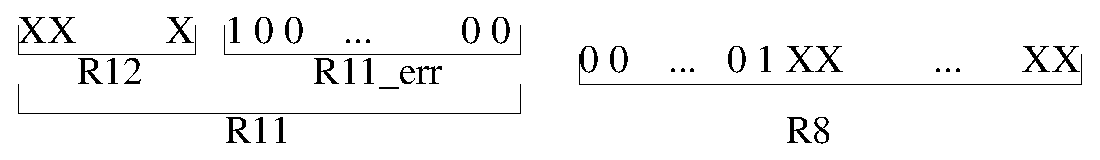
\includegraphics[width=0.5\textwidth]{rnd_to_nearest_pp.eps}
%   \end{center} 
%\end{figure}

%\begin{figure}[!htb]  
%  \begin{center}
%    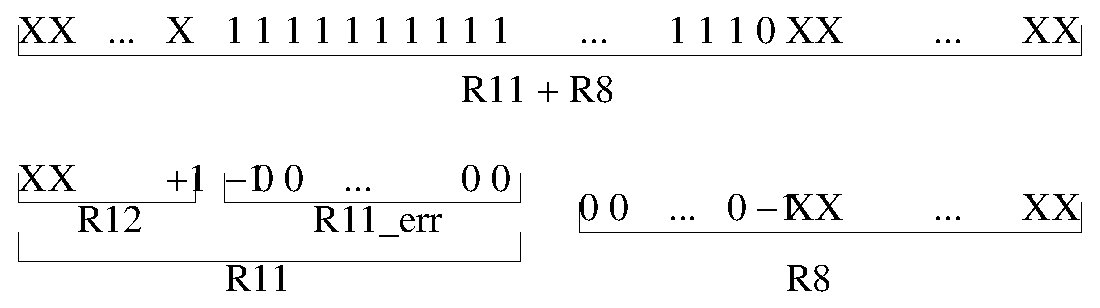
\includegraphics[width=0.5\textwidth]{rnd_to_nearest_mm.eps}
%  \end{center} 
%\end{figure}

\begin{figure}[ht] \begin{center}
\input{fig_exp/rnd_to_nearest.pstex_t}
\caption{Description of problem with rounding to nearest of a subnormal number.
  \label{chap4:fig:rnd_to_nearest}}
\end{center}\end{figure}


 
\subsection{Rounding toward $+ \infty$}
\begin{lstlisting}[caption={Test if rounding toward $+ \infty$ is possible}]
static const union{int i[2]; double d;}
#ifdef BIG_ENDIAN
 _two1000    = {0x7E700000, 0x00000000}, /*  1.07150860718626732095e301  */
 _twom1000   = {0x01700000, 0x00000000}, /*  9.33263618503218878990e-302 */
#else
 ...
#endif
#define two1000    _two1000.d
#define twom1000   _twom1000.d


int errd        = 71303168;                    /* 68 * 2^20 */  

int    exp_R11;
union {int i[2]; long long int l; double d;} R12;

/* Result = (R11 + R8) */

exp_R11 = (HI(R11) & 0x7ff00000) - errd;

if ((HI(R8) & 0x7ff00000) > exp_R11){      (*@ \label{exp:code:pinf:0} @*)
  /* We are able to round the result */
  if (k > -1020){                          
    if (k < 1020){                         
      HI(R11) += (k<<20);                  
    }else {
      /* We are close to + Inf */
      HI(R11) += ((k-1000)<<20);           
      R11 *= two1000;
    }
    if (HI(R8) > 0){                       (*@ \label{exp:code:pinf:1} @*)
      R12.d  = R11;
      R12.l += 1;
      R11    = R12.d;
    }
    return R11;
  }else {
    /* We are with subnormal number */
    HI(R11) += ((k+1000)<<20);          
    R12.d    = R11 * twom1000;              (*@ \label{exp:code:pinf:2} @*)

    HI(st2mem) = R12.i[HI] ;     
    LO(st2mem) = R12.i[LO]       

    R11 -= st2mem * two1000;                (*@ \label{exp:code:pinf:3} @*)
    if ((HI(R11) > 0)||((HI(R11) == 0)&&(HI(R8) > 0))) R12.l += 1;(*@ \label{exp:code:pinf:5} @*)

    return R12.d;
  }
}else {
  /* Difficult case */
  su_exp(x);
}
\end{lstlisting}


\begin{preuve}

The program used to check whether correct rounding toward $+ \infty$ is possible is similar to the one used with rounding to nearest.

\begin{longtable}[c]{@{line }p{0.08\textwidth}p{0.81\textwidth}}
% en cas de cesure c'est ce que l'on place 
% en debut de page
\endhead
% en fin de page
\endfoot 
% en fin de derniere page
\endlastfoot 
\ref{exp:code:pinf:0} & 
This test is valid even if the final result is a subnormal number.
\\

\ref{exp:code:pinf:1} &
We add $1 ulp$ to the result if $R8$ is positive. 
\\

\ref{exp:code:pinf:3} &
Like for rounding to nearest, the quantity $R11$ represent the rounding error that come from the operation $R11* twom1000$ in line \ref{exp:code:pinf:2}.
\\

\ref{exp:code:pinf:5} &
This test check whether the error from line \ref{exp:code:pinf:2} is strictly positive or if it is equal to zero and if $R8$ is strictly positive. If we are in one of these two cases, by definition of rounding toward $+ \infty$, we need to add $1 ulp$ to the result.
\end{longtable}
\end{preuve}


 
\subsection{Rounding toward $- \infty$}

\begin{lstlisting}[caption={Test if rounding toward $- \infty$ is possible},firstnumber = 144]
static const union{int i[2]; double d;}
#ifdef BIG_ENDIAN
 _two1000    = {0x7E700000, 0x00000000}, /*  1.07150860718626732095e301  */
 _twom1000   = {0x01700000, 0x00000000}, /*  9.33263618503218878990e-302 */
#else
 ...
#endif
#define two1000    _two1000.d
#define twom1000   _twom1000.d

int errd        = 71303168;                    /* 68 * 2^20 */  

int    exp_R11;
union {int i[2]; long long int l; double d} R12;
 
/* R�sult = (R11 + R8) */

exp_R11 = (HI(R11) & 0x7ff00000) - errd;

if ((HI(R8) & 0x7ff00000) > exp_R11){
  /* We are able to round the result */
  if (k > -1020){                          
    if (k < 1020){                         
      HI(R11) += (k<<20);                  
    }else {
      /* We are close to + Inf */
      HI(R11) += ((k-1000)<<20);           
      R11 *= two1000;
    }
    if (HI(R8) > 0){
      R12.d  = R11;
      R12.l += 1;
      R11    = R12.d;
    }
    return R11;
  }else {
    /* We are with subnormal number */
    HI(R11) += ((k+1000)<<20);             
    R12.d    = R11 * twom1000;             

    HI(st2mem) = R12.i[HI];                  
    LO(st2mem) = R12.i[LO];                  

    R11 -= st2mem * two1000;               
    if ((HI(R11) < 0)||((HI(R11) == 0)&&(HI(R8) < 0))) R12.l -= 1;

    return R12.d;
  }
}else {
  /* Difficult case */
  su_exp(x);
}
\end{lstlisting}



\begin{preuve}

The program used to check whether correct rounding toward $- \infty$ is possible is similar to the previous one and it work for similar reasons.
\end{preuve}


 
\subsection{Rounding toward $0$} 
The program used to check whether correct rounding toward $0$ is possible is identical to the one used for rounding to $- \infty$ because $\exp(x)$ is a positive function.

%%
%% 
%%
\section{Accurate phase}
\label{section:accurate_phase}
When the previous computation failed, it mean that the rounding of the result is difficult to get. We need to use more accurate methods :
\begin{itemize}
\item
 $sn\_exp$ with rounding to nearest,
\item
 $su\_exp$ with rounding toward $+\infty$,
\item
 $sd\_exp$ with rounding toward $-\infty$,
\end{itemize}

These methods are based on SCS library \cite{SCSweb}, with $30$ bits of precision per digits and $8$ digits per vector. The guarantee precision with this format is $211$ bits at least. Even if there is no proof for these operators yet, the proof for correct rounding of the exponential only request the following property  that are easy to check and/or satisfy :

\begin{propriete}(Addition)
Let $a \boxplus b$ represent the multiprecision operation performing an addition between $a$ and $b$ with at least $210$ bits of precision for the result. Like for double precision floating point number, the scs addition may leads to a cancellation. We have :
$$
a+ b = (a \boxplus b).(1+\epsilon_{-211})
$$
\end{propriete}

\begin{propriete}(Multiplication)
Let $a \boxtimes b$ represent the multiprecision operation performing a multiplication between $a$ and $b$ with at least $210$ bits of precision for the result. This operation do not produce a cancellation.
$$
a\times b = (a \boxtimes b).(1+\epsilon_{-211})
$$
\end{propriete}



\subsection{Overview of the algorithm}
Here is the algorithm used for the second part of the evaluation :
\begin{enumerate}
\item
{\bf No special case handeling} \\
For this part, we assume that test for special case handeling have been done.
\item
{\bf Range reduction} \\
We compute the reduced argument $r$ and the integer $k$ such that :
$$
r = \frac{x - k . \ln(2)}{512}
$$

with
$\frac{-\ln(2)}{1024} \leq r \leq \frac{-\ln(2)}{1024}$

such that
$$
\exp(x) = \exp(r)^{512} \times 2^{k}
$$


\item
{\bf Polynomial evaluation} \\
We compute the polynom $P(r)$ of degree 10 :
$$
\exp(r) = (1 + r + P(r)).(1+ \epsilon_{-164})
$$

\item
{\bf Powering the result} \\
$\exp(r)^{512} = \left(\left(\left(\left(\left(\left(\left(\left(\exp(r)^2\right)^2\right)^2\right)^2\right)^2\right)^2\right)^2\right)^2\right)^2$



\item
{\bf Reconstruction} \\
$$
\exp(x) = \exp(r)^{512}. 2^{k} . (1+\epsilon)
$$
avec $|\epsilon| \leq 2^{-163} $
\end{enumerate}

We have choosen this evaluation scheme, because the reconstruction step use the squaring multiprecision operator. This operator facilitate the error computation and is very economic : its cost is $0.7$ times the one of a true multiprecision multiplication.

We will notice that there exist an alternative to the squaring solution. We can tabulate values $2^{\frac{N}{512}}$ for $N=1,2,\ldots,511$ and use the formulae $\exp(x) = \exp(r) \times 2^{N} \times 2^{\frac{M}{512}}$ with $k=M+N/512$. However we prefer the squaring method that do not request the storage of SCS number and the associated quantity of memory.



\subsection{Function's call}
With Lef\`evre worst cases on table makers dilemma we get the following theorem :

\begin{theorem}(Correct rounding for the exponential)
Let $y$ be the exact value of the exponential of a floating-point number in double precision $x$. Let $y^*$ be an approximation of $y$ such that the distance between $y$ and $y^*$ be bounded by $\epsilon$. Then if $\epsilon \leq 2^{-157}$, for each of the four rounding mode, rounding $y^*$ is equivalent to rounding $y$;
\end{theorem}

To round the multiprecision result in SCS format depending on the rounding mode, we use the following procedure (\texttt{scs\_get\_d}, \texttt{scs\_get\_d\_pinf}, \texttt{scs\_get\_d\_minf}). 

\subsubsection{Rounding to nearest}

\begin{lstlisting}[caption={Compute the rounding to nearest of the exponential in multiprecision},firstnumber=1]
double sn_exp(double x){ 
  scs_t res_scs;
  scs_db_number res;

  exp_SC(res_scs, x);
  scs_get_d(&res.d, res_scs);  res.d = x;

  return res.d;
}
\end{lstlisting}



\subsubsection{Rounding toward $+ \infty$}

\begin{lstlisting}[caption={Compute the rounding toward $+ \infty$ of the exponential in multiprecision},firstnumber=1]
double su_exp(double x){ 
  scs_t res_scs;
  scs_db_number res;
  
  exp_SC(res_scs, x);
  scs_get_d_pinf(&res.d, res_scs);
  return res.d;
}
\end{lstlisting}



\subsubsection{Rounding toward $- \infty$}

\begin{lstlisting}[caption={Compute the rounding toward $- \infty$ of the exponential in multiprecision},firstnumber=1]
double sd_exp(double x){ 
  scs_t res_scs;
  scs_db_number res;
  
  exp_SC(res_scs, x);
  scs_get_d_minf(&res.d, res_scs);
  return res.d;
}
\end{lstlisting}



\subsection{Software}
The function $exp\_SC$ approximate the exponential of $x$ with $163$ bits of precision and put the result in $res\_scs$.

\begin{lstlisting}[caption={Compute the exponential in multiprecision},firstnumber=1]
void exp_SC(scs_ptr res_scs, double x){
  scs_t sc1, red;
  scs_db_number db;
  int i, k;


  /* db.d = x/512  (= 2^9)  */
  
  db.d = x;                                    (*@ \label{exp:mp:0} @*)
  db.i[HI] -= (9 << 20);                (*@ \label{exp:mp:1} @*) 
  scs_set_d(sc1, db.d);                        (*@ \label{exp:mp:2} @*)
  
  
  DOUBLE2INT(k, (db.d * iln2_o512.d));         (*@ \label{exp:mp:3} @*) 
 
  /* 1) Range reduction */
  
  scs_set(red,     sc_ln2_o512_ptr_1);;        (*@ \label{exp:mp:4} @*)             
  scs_set(red_low, sc_ln2_o512_ptr_2);         (*@ \label{exp:mp:4b} @*)      
  if (k>0){
    scs_mul_ui(red,      (unsigned int) k);
    scs_mul_ui(red_low,  (unsigned int) k);
  }else {
    scs_mul_ui(red,      (unsigned int)(-k));
    scs_mul_ui(red_low,  (unsigned int)(-k));
    red->sign *= -1;
    red_low->sign *=-1;
  }                                            (*@ \label{exp:mp:5} @*)

  scs_sub(red, sc1, red);                      (*@ \label{exp:mp:6} @*)
  scs_sub(red, red, red_low);                  (*@ \label{exp:mp:6b} @*)

  
  /* 2) Polynomial evaluation */               (*@ \label{exp:mp:7} @*)
   
  scs_mul(res_scs, constant_poly_ptr[0], red);
  for(i=1; i< 10; i++){                       
    scs_add(res_scs, constant_poly_ptr[i], res_scs);
    scs_mul(res_scs, red, res_scs);            
  }
  
  scs_add(res_scs, SCS_ONE, res_scs);          
  scs_mul(res_scs, red, res_scs);
  scs_add(res_scs, SCS_ONE, res_scs);          (*@ \label{exp:mp:8} @*)  

  /* 3) Powering the result exp(r)^512  */
  
  for(i=0; i<9; i++){                          (*@ \label{exp:mp:9} @*)
    scs_square(res_scs, res_scs);
  }

  /* 4) Multiplication by 2^k */
  
  res_scs->index += (int)(k/30);               (*@ \label{exp:mp:10} @*)
  if ((k%30) > 0) 
    scs_mul_ui(res_scs, (unsigned int) (1<<((k%30))));
  else if ((k%30) < 0){
    res_scs->index --;
    scs_mul_ui(res_scs, (unsigned int) (1<<((30+(k%30)))));
  }                                            (*@ \label{exp:mp:11} @*)

}

\end{lstlisting}



\begin{preuve}
\begin{longtable}[c]{@{line }p{0.08\textwidth}p{0.81\textwidth}}
% en cas de cesure c'est ce que l'on place 
% en debut de page
\endhead
% en fin de page
\endfoot 
% en fin de derniere page
\endlastfoot 
\ref{exp:mp:0}& $db.d = x$
\\
\ref{exp:mp:1}& 
This operation divide  $db.d$ by $512=2^9$ and is valid under the condition that $db.d$, and consequently $x$, do not represent a special values (subnormal, infinity, NaN). Condition that is satisfied because special case have been treated during the quick phase.

\\
\ref{exp:mp:2}& 
$sc1$ is a $211$ bits multiprecision number such that :
\begin{prop}
  \label{chap3:exp:mp:prop0}
 $sc1=db.d = \frac{x}{512}$ exactly
\end{prop}
\\
\ref{exp:mp:3}& $iln2\_o512.d$ is a double precision floating-point number such that :
$iln2\_o512.d = \frac{512}{\ln{2}}(1 + \epsilon_{-54})$. This line put in $k$ the closest integer of $db.d \otimes \frac{512}{\ln{2}}$. We use the property of $DOUBLE2INT$ which convert a floating-point number in an integer with rounding to nearest.

Moreover $k$ satisfy the following property :
\begin{prop}
  \label{chap3:exp:mp:prop1}
  $$
\lfloor \frac{x}{\ln 2} \rfloor  \leq k \leq   \lceil \frac{x}{\ln 2} \rceil
   ~~~ \mbox{et} ~~~   -1075 \leq |k| \leq 1025
$$
\end{prop}
And $k$ is a $11$ bits integer.
\\
\ref{exp:mp:4}, \ref{exp:mp:4b}&
By construction we have :
$$red + red\_low = \frac{\ln 2}{512}(1 + \epsilon_{-450})$$
and $red$ is construct in order to make the multiplication of $red$ by $k$ exact if $|k| \leq 2^{11}$.

\\
\ref{exp:mp:5}&
At the end of the test on $k$ we have : 
$red + red\_low = k \otimes \frac{\ln 2}{512}(1 + \epsilon_{-450})$

with $|k| < 2^{11}$, then :
\begin{prop}
  \label{chap3:exp:mp:prop2}
$$red  + red\_low = k \times \frac{\ln 2}{512}(1 + \epsilon_{-411})$$
\end{prop}
\\
\ref{exp:mp:6},\ref{exp:mp:6b}&
By the properties \pref{chap3:exp:mp:prop0} and \pref{chap3:exp:mp:prop2} we have :
\begin{prop}
  \label{chap3:exp:mp:prop3}
$red = \frac{x}{512} \ominus \left( k \times \frac{\ln 2}{512} \right) (1 + \epsilon_{-411})$
\end{prop}

In addition we have seen in the quick phase that at most $58$ bits could be cancelled, during this subtraction.
\begin{prop}
  \label{chap3:exp:mp:prop4}
$|red| \leq \frac{\ln 2}{1024} \leq 2^{-10}$,

$red = \frac{x}{512} - k \times \frac{\ln 2}{512}  + \epsilon_{-211} $
\end{prop}
\\
\ref{exp:mp:7}-\ref{exp:mp:8}&
We now perform the polynomial evaluation where the coefficient have the following properties.
\begin{prop}
  \label{chap3:exp:mp:prop5}
$|constant\_poly\_ptr[0]=c_0| \leq 2^{-25}$, $|constant\_poly\_ptr[1]=c_1| \leq 2^{-21}$,
$|constant\_poly\_ptr[2]=c_2| \leq 2^{-18}$, $|constant\_poly\_ptr[3]=c_3| \leq 2^{-15}$,
$|constant\_poly\_ptr[4]=c_4| \leq 2^{-12}$, $|constant\_poly\_ptr[5]=c_5| \leq 2^{-9}$,
$|constant\_poly\_ptr[6]=c_6| \leq 2^{-6}$,  $|constant\_poly\_ptr[7]=c_7| \leq 2^{-4}$,
$|constant\_poly\_ptr[8]=c_8| \leq 2^{-2}$,  $|constant\_poly\_ptr[9]=c_9| \leq 2^{-1}$
\end{prop}


We have :
\begin{itemize}
\item $P_0=c_1 \boxplus (red \boxtimes c_0)$   thus $|P_0| \leq 2^{-20}$ et $P_0 = c_1 + (red \times c_0 ) + \epsilon_{-231}$
\item $P_1=c_2 \boxplus (red \boxtimes P_0)$   thus $|P_1| \leq 2^{-17}$ et $P_1 = c_2 + (red \times P_0 ) + \epsilon_{-228}$
\item $P_2=c_3 \boxplus (red \boxtimes P_1)$   thus $|P_2| \leq 2^{-14}$ et $P_2 = c_3 + (red \times P_1 ) + \epsilon_{-225}$
\item $P_3=c_4 \boxplus (red \boxtimes P_2)$   thus $|P_3| \leq 2^{-11}$ et $P_3 = c_4 + (red \times P_2 ) + \epsilon_{-222}$
\item $P_4=c_5 \boxplus (red \boxtimes P_3)$   thus $|P_4| \leq 2^{-8}$ et $P_4 = c_5 + (red \times P_3 ) + \epsilon_{-219}$
\item $P_5=c_6 \boxplus (red \boxtimes P_4)$   thus $|P_5| \leq 2^{-5}$ et $P_5 = c_6 + (red \times P_4 ) + \epsilon_{-216}$
\item $P_6=c_7 \boxplus (red \boxtimes P_5)$   thus $|P_6| \leq 2^{-3}$ et $P_6 = c_7 + (red \times P_5 ) + \epsilon_{-214}$
\item $P_7=c_8 \boxplus (red \boxtimes P_6)$   thus $|P_7| \leq 2^{-1}$ et $P_7 = c_8 + (red \times P_6 ) + \epsilon_{-212}$
\item $P_8=c_9 \boxplus (red \boxtimes P_7)$   thus $|P_8| \leq 1 + 2^{-10} $ et $P_8 = c_9 + (red \times P_7 ) + \epsilon_{-211}$
\item $P_9=1   \boxplus (red \boxtimes P_8)$   thus $|P_9| \leq 1 + 2^{-9}$ et $P_9 = 1   + (red \times P_8 ) + \epsilon_{-210}$
\item $P_{10}=1   \boxplus (red \boxtimes P_9)$ thus $|P_{10}| \leq 1 + 2^{-8}$ et $P_{10} = 1   + (red \times P_9) + \epsilon_{-210}$
\end{itemize}

Therefore :
$$
res\_scs = P_{10} + \epsilon_{-208}
$$ 

We build the polynom such that  
$$\exp(r) = (1 + r + c_9. r^2 + \cdots + c_0 . r^{11}).(1 + \epsilon_{-164})$$
Therefore

$|res\_scs| \leq 1 + 2^{-8}$
with

$\exp(red) = (res\_scs  + \epsilon_{-208}).(1 + \epsilon_{-164})$
\\

\ref{exp:mp:9}&
We perform a squaring of the result $9$ times, that correspond to powering the result to the power $512$. 
At each iteration we perform a rounding error equal to $\epsilon_{-211}$.

Finally :

$|res\_scs| \leq  2^{3}$
and

$\exp(x) = 2^k. (res\_scs  + \epsilon_{-199}).(1 + \epsilon_{-164})$
\\
\ref{exp:mp:10}-\ref{exp:mp:11}&
With these lines we perform the multiplication of $res\_scs$ by $2^k$. This multiplication is done by a shift on the index of $k/30$, where $30$ correspond to the number of bits used within a multiprecision number. This shift is exact. Then a multiplication of $res\_scs$ by $2$ to the power the rest of the euclidian division of $k$ by $30$ is done. At the end of these instructions we have :
$$\exp(x) = (res\_scs).(1 + \epsilon_{-163})$$

\\

\end{longtable}
\end{preuve}




%%%%%%%%%%%%%%%%%%%%%%%%%%%%%%%%%%%%%%%%%%%%%%%%%%%%%%%%%%%%%
\section{Analysis of the exponential}
\label{section:exp_results}

\subsection{Test conditions}

Table \ref{tbl:systems} lists the combinations of processor, OS and
default \texttt{libm} used for our tests.
\begin{table}[!htb]
\begin{center}
\renewcommand{\arraystretch}{1.2}
\begin{tabular}{|c||c|c|c|}
\hline
Processor        & OS & compiler & default \texttt{libm} \\
\hline
\hline
Pentium III      & Debian GNU/Linux & gcc-2.95          & \texttt{glibc}, derived from \texttt{fdlibm} \\ 
\hline
UltraSPARC IIi   & SunOS 5.8        & gcc-2.95          & \texttt{fdlibm} \\
\hline
Xeon (Pentium 4) & Debian GNU/Linux & gcc-2.95          & \texttt{glibc}, derived from \texttt{fdlibm}\\
\hline
PowerPC G4       & MacOS 10.2       & gcc-2.95          & Apple specific \\
\hline
Itanium          & Debian GNU/Linux & gcc-2.95, gcc-3.2 & Intel optimized \\
\hline
\end{tabular}
\end{center}
\caption{The systems tested
  \label{tbl:systems}}
\end{table}

The following presents tests
performed under such conditions as to suppress most of the impact of
the memory hierarchy: A small loops performs 10 identical calls to
the function, and the minimum timing is reported, ensuring that both
code and data have been loaded in the cache, and that interruptions by
the operating system do not alter the timings.

These timings are taken on random values between $-745$ and $+744$,
which is the practical range for the exponential. We also report the
timing for the worse case for the correct rounding in rounding to
nearest mode of the exponential, which is
$x=7.5417527749959590085206221e-10$.

Our libray was tuned to take into account the adequation of the evaluation scheme to the memory hierarchies of current processors (our program for the exponential evaluation uses $2.8$Kbytes of table for the four rounding modes, whereas the one from \emph{fdlibm} use $13$Kbytes). However we do not have tested the impact over performance of this concern and is part of our futur works. 

\subsection{Results}

Tables \ref{tbl:exp_abstime} gives a summary of the timings of the
various libraries. The \accurate\ phase is called about 2 times out of 100000.


\begin{table}[!htb]
\begin{center}
\renewcommand{\arraystretch}{1.2}
\begin{tabular}{|l|r|r|r|}
\hline
 \multicolumn{4}{|c|}{Pentium 4 Xeon / Linux Debian sarge / gcc 3.3}   \\ 
 \hline
 \hline
 \texttt{libm}           & 236          & 5528          &        365 \\ 
 \hline
  \texttt{mpfr}          & 14636        & 204736        &      23299 \\ 
 \hline
  \texttt{libultim}      & 44           & 3105632       &        210 \\ 
 \hline
 \texttt{crlibm}         & 316          & 41484         &        432 \\ 
 \hline
 \hline
  \multicolumn{4}{|c|}{PowerPC G4 / MacOS X / gcc2.95}   \\
 \hline
                         & min time      & max time      & avg time \\
 \hline
 \texttt{libm}           & 7            & 14            &         12 \\
 \hline
  \texttt{mpfr}          & 972          & 2819          &       1367 \\
 \hline
  \texttt{libultim}      & 8            & 169390        &         12 \\
 \hline
 \texttt{crlibm}         & 4            & 916           &         15 \\
 \hline
\end{tabular}
\end{center}
\caption{Absolute timings for the exponential (arbitrary units)
  \label{tbl:exp_abstime}}
\end{table}





\subsection{Analysis}

\subsubsection*{Processor-specific libraries}
Documentation\cite{HarKubStoTan99} from Intel labs claim to provide an
exponential in only $48$ cycles. This performance is possible through
the wide use of non portable tricks such as inverse approximation,
fused multiply and add and double extended precision.  However, our
tests show that the environmental cost (mainly the cost of a function
call) is about $80$ clock cycles! Our tests have also shown that there
exists a slower path that takes up to $2767$ clock cycles, which is $14$ times slower. This path
seems to be taken very often since the average cost is $1.5$ times
more expensive than the smallest  execution time.

The same conclusion can be done for the mathematical library used on
Ultra-SPARC IIi system, where there exists a path $13$ times slower
than a normal execution.

These two observations show that our two-step procedure, with a much
slower second step, could be viable in the commercial world.

The mathematical library used on the PowerPC G4 with gcc is the one
from Apple. This library do not provide correct rounding and is $1.1$
slower than the version provided with \emph{crlibm}. It is, however,
the most accurate of the tested libraries.


\subsubsection*{The cost of correct rounding}

The \emph{libutlim} library provides correct rounding for an average
cost between $0.9$ (on a Pentium III) and $1.8$ (on an Itanium) times
the cost of the standard library. Our exponential give a result for an
average cost between $0.91$ (on Power-PC) and $2.66$ (on Ultra-SPARC
IIi) times the cost of the standard library, which is reasonable. On
the other hand, MPFR provide correct rounding for an average cost
between $13.5$ (on Power-PC) and $153$ (on Itanium) compared to the
\emph{libm}. 

The main advantage of \emph{crlibm} over \emph{libutlim} is the upper
bound on the execution time. On our tests, this bound for
\emph{crlibm} is $147$ times the average \emph{libm} cost, whereas for
\emph{libtultim} this bound goes up to $14499$ times the average
\emph{libm} cost. Our two steps strategy fully benefits from knowing
bounds on correct rounding worst cases.

We notice that our second step is in average $3$ times faster than the
multiprecision library MPFR. It shows that our multiprecision
operators from \emph{scslib}, hand tuned for $200$ bits of precision
perfectly fulfill the performance requirement of the second step.


\subsubsection*{Relations between the two steps of \emph{crlibm}}

Our second phase is $30$ times slower than the first step and is
called only once over $2^{13}$. The cost of the second step over the
average cost is :

$$
\frac{1 \times (2^{13}-1) + 30 \times 1}{2^{13}} = 1.003540039
$$
which corresponds to a $0.35\%$ overhead. This small overhead in
average  means that a possible performance improvement
is to reduce the precision of the first step, and by the same way the
number of instructions, to increase to number of time that the second
step is called. It will also make the proof simpler.


%%%%%%%%%%%%%%%%%%%%%%%%%%%%%%%%%%%%%%%%%%%%%%%%%%%%%%%%%%%%%
\section{Conclusion and perspectives}


 It is obvious from our performance measurements that our first step is
too accurate and too slow for a balanced average time. We will take
this experience into consideration when writing first steps for other
functions. The IBM library seems to get a better balance although its
second and later steps are much slower. Its code, unfortunately, is
little documented and difficult to prove.

Writing the proofs is a very time-consuming task, which could be
partially automated for one step which is common to most function: The
accumulation of error terms in order to compute the final error.




 \chapter{The trigonometric functions \label{chap:trigo}}
  This chapter is contributed by F. de~Dinechin with assistance of C.
Daramy-Loirat and D. Defour.

\section*{Introduction}
This chapter describes the implementations of sine, cosine and
tangent, as they share much of their code. The proof sketch below is
supported by the Maple script \texttt{maple/trigo.mpl} and the Gappa
scripts \texttt{maple/trigoSinCosCase3.gappa} and
\texttt{maple/trigoTanCase2.gappa} of the \crlibm\ distribution, which
implement the computations of error bounds and validity bounds for the
various algorithmic paths described here.

\section{Overview of the algorithms}

\subsection{Exceptional cases}

The three trigonometric functions return NaN for infinite and NaN
arguments, and are defined otherwise. 

An argument based on continued fractions to find the worst cases for
range reduction may also be used to show that the sine and cosine of a
floating-point number outside of $[-1,1]$ is always larger than
$2^{-150}$, and therefore never flushes to zero nor to subnormal (see
\cite{Muller97} p. 151 and following). Therefore
$\tan(x)=\sin(x)/\cos(x)$ also remains larger than $2^{-150}$.

This has two important consequences:

\begin{itemize}
\item as the output a trigonometric function is never a subnormal except for
  inputs around zero (for which the value to return is trivial
  anyway), we can safely use the rounding tests from Section
  \ref{section:testrounding}.

\item as the cosine never flushes to zero, the tangent of a floating-point
  number is never an infinity.
\end{itemize}

For very small arguments,
\begin{itemize}
\item $\sin(x) = x-x^3/6 + O(x^5) = x(1-x^2/6) + O(x^5)$ where
  $O(x^5)$ has the sign of $x$. Therefore $\sin(x)$ is rounded to $x$
  or one of its floating-point neighbours $|x|<2^{-26}$.
\item $\cos(x) = 1-x^2/2 + O(x^4)$ where $O(x^4)$ is positive.
  Therefore $\cos(x)$ is rounded to $1$ in RN and RU mode if
  $x<\sqrt{2^{-53}}$. In RD and RZ modes, we have $\cos(0)=1$ and
  $\cos(x)=1-2^{-53}$ for $|x|<2^{-26}$.
\item $\tan(x) = x+x^3/3 + O(x^5) = x(1+x^2/3) + O(x^5)$ where
  $O(x^5)$ has the sign of $x$. Therefore $\tan(x)$ is rounded to $x$
  or one of its neighbours for all the rounding  modes if $|x|<2^{-27}$.
\end{itemize}


\subsection{Argument reduction}

Most implementations of the trigonometric functions have two steps of argument reduction: 
\begin{itemize}
\item first the input number $x$ is reduced to $y\in
  [-\frac{\pi}{4}, \frac{\pi}{4}]$, with reconstruction using periodicity and
  symmetry properties,
\item then the reduced argument is further broken down as $y=a+z$,
  with reconstruction using the formula for $\sin(a+z)$ and
  $\cos(a+z)$, using tabulated values of $\sin(a)$ and
  $\cos(a)$
\end{itemize}

We chose to implement argument reduction in one step only, which
computes an integer $k$ and a reduced argument y such that

\begin{equation}
  x = k\frac{\pi}{256} + y\label{eq:trigoargred}
\end{equation}
where $k$ is an integer and  $ |y| \leq {\pi}/{512}$.
This step computes $y$ as a double-double: $y\approx y_h+y_l$. 

In the following we note $$a=k\pi/256.$$ 

Then we read off a table 

$$sa_h+sa_l \approx sin(a)$$
$$ca_h+ca_l \approx cos(a)$$

Only 64 quadruples $(sa_h,sa_l,ca_h,ca_l)$ are tabulated (amounting to
$64\times 8 \times 4 = 2048$ bytes), the rest is obtained by
periodicity and symmetry, implemented as masks and integer operations
on the integer $k$. For instance,  $a \mod 2\pi$ is implemented by $k \mod 512$,
$\pi/2-a$ is implemented as $128-k$, etc.



Then we use the reconstruction steps:

\begin{equation}        
  \sin(x) = \sin(a + y) =  \cos(a) \sin(y) +  \sin(a) \cos(y) 
  \label{eq:sinapy}
\end{equation}

\begin{equation}
  \cos(x) = \cos(a + y) = \cos(a) \cos(y) -  \sin(a) \sin(y) 
  \label{eq:cosapy}
\end{equation}

\begin{equation} 
  tan(x) = \frac{\sin(x)}{\cos(x)} 
  \label{eq:tanapy}
\end{equation}


\subsection{Polynomial evaluation}


To implement the previous equations, $\cos(y)$ and $\sin(y)$ are
computed as unevaluated $1+t_c$ and $(y_h+y_l)(1+t_s)$ respectively,
where $t_c$ and $t_s$ are doubles computed using a polynomial
approximation of small degree:

\begin{itemize}
\item $t_s = y^2(s_3 + y^2(s_5 + y^2s_7)))$ with $s3$, $s5$ and
$s7$ the Taylor coefficients.
\item $t_c = y^2(c_2 + y^2(c_4 + y^2c_6))$ with $c2$, $c4$ and $c6$ the
Taylor coefficients (or a more accurate minimax approximation).
\end{itemize}



\subsection{Reconstruction}

\subsubsection{Sine}
According to equation (\ref{eq:sinapy}), we have to compute: 
 \begin{eqnarray*}
  \sin(a+y) &=& \sin(a) \cos(y)  + \cos(a)\sin(y)  \\
  & \approx& (sa_h+sa_l)(1+t_c) + (ca_h+ca_l)(y_h+y_l)(1+t_s)
\end{eqnarray*}


Figure~\ref{fig:sine-reconstruction} shows the worst-case respective
orders of magnitude of the terms of this sum. The terms completely to the
right of the vertical bar will be neglected, and a bound on the
error thus entailed is computed in the following. Note that the term
$ca_hy_h$ has to be computed exactly by a Mul12.

Finally the reconstruction consists of adding together the lower-order
terms in increasing order of magnitude, and computing the
double-double result by an Add12.

\begin{figure}[htbp]    
  \begin{center}
    \small
    \setlength{\unitlength}{3ex}
      \framebox{
        \begin{picture}(22,9)(-3,-4.2)
          \put(9.5,4){\line(0,-1){8}}  %\put(9,4){$\epsilon$}
          
          \put(4,3.2){$sa_h$} \put(0.05,3){\framebox(7.9,0.7){}}
          \put(12,3.2){$sa_l$}  \put(8.05,3){\framebox(7.9,0.7){}}
          
          \put(6,2.2){$sa_ht_c$} \put(2.05,2){\framebox(7.9,0.7){}}
          \put(14,2.2){$sa_lt_c$}  \put(10.05,2){\framebox(7.9,0.7){}}

          \put(4.5,1.2){$ca_hy_h$} \put(0.55,1){\framebox(7.9,0.7){}}
          \put(12.5,1.2){$ca_hy_h$}  \put(8.55,1){\framebox(7.9,0.7){}}

          \put(11.5,0.2){$ca_hy_l $}  \put(7.55,0){\framebox(7.9,0.7){}}
          \put(11.5,-0.8){$ca_ly_h $}  \put(7.55,-1){\framebox(7.9,0.7){}}

         \put(6.5,-1.8){$ca_hy_ht_s$} \put(2.55,-2){\framebox(7.9,0.7){}}
         \put(13.5,-2.8){$ca_hy_lt_s $}  \put(9.55,-3){\framebox(7.9,0.7){}}
         \put(13.5,-3.8){$ca_ly_ht_s $}  \put(9.55,-4){\framebox(7.9,0.7){}}
        
       \end{picture}
     }
   \end{center}
   \caption{The sine reconstruction}
   \label{fig:sine-reconstruction}
 \end{figure}
 
 

\subsubsection{Cosine}
According to equation (\ref{eq:cosapy}), we have to compute in double-double precision:
 \begin{eqnarray*}
  \cos(a+y) &=& \cos(a) \cos(y)  - \sin(a)\sin(y)  \\
  & \approx& (ca_h+ca_l)(1+t_c) - (sa_h+sa_l)(y_h+y_l)(1+t_s)
\end{eqnarray*}

This is similar to the case of the sine, and the respective orders of
magnitude are given by Figure~\ref{fig:sine-reconstruction}.

\begin{figure}[htbp]
  \begin{center}
    \small \setlength{\unitlength}{3ex} \framebox{
      \begin{picture}(22,9)(-3,-4.2)
        \put(9.5,4){\line(0,-1){8}}
%        \put(9,4){$\epsilon$}
  
        \put(4,3.2){$ca_h$} \put(0.05,3){\framebox(7.9,0.7){}}
        \put(12,3.2){$ca_l$}  \put(8.05,3){\framebox(7.9,0.7){}}

        \put(6,2.2){$ca_ht_c$} \put(2.05,2){\framebox(7.9,0.7){}}
        \put(14,2.2){$ca_lt_c$}  \put(10.05,2){\framebox(7.9,0.7){}}

        \put(4.5,1.2){$-sa_hy_h$} \put(0.55,1){\framebox(7.9,0.7){}}
        \put(12.5,1.2){$-sa_hy_h$}  \put(8.55,1){\framebox(7.9,0.7){}}

        \put(11.5,0.2){$-sa_hy_l $}  \put(7.55,0){\framebox(7.9,0.7){}}
        \put(11.5,-0.8){$-sa_ly_h $}  \put(7.55,-1){\framebox(7.9,0.7){}}

        \put(6.5,-1.8){$-sa_hy_ht_s$} \put(2.55,-2){\framebox(7.9,0.7){}}
        \put(13.5,-2.8){$-sa_hy_lt_s $}  \put(9.55,-3){\framebox(7.9,0.7){}}
        \put(13.5,-3.8){$-sa_ly_ht_s $}  \put(9.55,-4){\framebox(7.9,0.7){}}
 
        \end{picture}
      }
    \end{center}\centering
    
    \caption{The cosine reconstruction}
    \label{fig:cosine-reconstruction}
  \end{figure}


\subsubsection{Tangent}

The tangent is obtained by the division of the sine by the cosine,
using the \texttt{Div22} procedure which is accurate to  $2^{-104}$.


\subsection{Precision of this scheme}

As we have $|y|<\pi/512<2^{-7}$, this scheme computes these functions
accurately to roughly $2^{53+13}$ bits, so these first steps are very
accurate. 
 

\subsection{Organisation of the code}


The code for argument reduction is shared by the three
trigonometric functions. It is detailed and proven in
Section~\ref{trigo:argred}.

Then there are four procedures (currently implemented as macros for
efficiency), respectively called \texttt{DoSinZero},
\texttt{DoCosZero}, \texttt{DoSinNotZero} and \texttt{DoCosNotZero}
which do the actual computation after argument reduction as per
Figures~\ref{fig:sine-reconstruction} and
\ref{fig:cosine-reconstruction}. The tangent function is computed by
dividing the sine by the cosine. These procedures are studied in
section \ref{trigo:auxiliary}.

Finally, each of the three trigonometric functions comes in four
variants for the four rounding modes. These four variants differ in
the beginning (special cases) and in the end (rounding), but share the
bulk of the computation. The shared computation is called
\verb!compute_trig_with_argred!.




\section{Details of argument reduction
\label{trigo:argred}}

\subsection{Basics about argument reduction}
The argument reduction or range reduction is the first step used in
the elementary function evaluation scheme. This step is required to
introduce a relation between the whole range of ieee double precision
number and the small range where the polynomial evaluation is accurate
enought. This relation between the input argument and the reduced
argument is called the range reduction step.

There is two categories of range reduction. First the multiplicative
reduction as we used for the logarithm, and the additive reduction as
the one we will use for the trigonometric function. Among this two,
only the additive reduction needs to be carrefully performed as it was
exhibit by K.C. Ng \cite{Ng1992}.

The additive reduction consists in adding or removing $N$ times a
certain constant $C$ from the input argument. For trigonometric
function this constant is usually equal to $\pi/2$ or
$\pi/4$. Therefor the naive range reduction based on machine precision
for trigonometric function consists in :


\begin{equation}
\begin{array}{rcl}
k    &=&  \lfloor \frac{x}{C} \rfloor \\
x^*  &=&  x-kC. \\
\end{array}
\label{chap6:eqn:rangereduction}
\end{equation}

When the input argument $x$ is close to $kC$, almost all the accuracy
is lost when preforming the substraction $x-kC$. When targeting
correctly rounded trigonometric function evaluation, we need to
determine how many bits can be lost with this operation. This number
is related to the knowledge of the closest input number $x$ to a
multiple of $C$. There exists an algorithm due to Kahan/Douglas and
based on continued fraction to compute this number and therefor the
number of bit lost. 

We used a Maple version from \cite{Muller97} to determine than up to
62 bits may be cancel up during range reduction for a ieee double
precision number. This Maple procedure is implemented as function
\texttt{WorstCaseForAdditiveRangeReduction} in
\texttt{maple/common-procedures.mpl} However this is not a concern
unless x is close to a multiple of $\pi/2$ (that is, $k \mod 128=0$):
in the general case the reconstruction will add some tabulated
non-zero value, so the error to consider in the range reduction is the
absolute error.  Only in the cases when $k \mod 128=0$ do we need to
have 62 extra bits to compute with. This is ensured by using a slower,
more accurate range reduction. As a compensation, in this case when $k
\mod 128=0$, there is no table to read and no reconstruction to
perform: a simple polynomial approximation to the function suffices.




\subsection{Details of the used scheme}

We have 4 possible range reductions, depending on the magnitude of the input number:

\begin{itemize}
\item Cody and Waite with 2 constants (the fastest),
\item Cody and Waite with 3 constants (almost as fast),
\item Cody and Waite with 3 constants in double-double and $k$ a
  64-bit int, and 
\item Payne and Hanek, implemented in SCS (the slowest).
\end{itemize}
Each of these range reductions except Payne and Hanek is valid for $x$
smaller than some bound. The computation of these bounds is detailed
below.

Section \ref{trigo:structargred} details the organization of this
multi-level argument reduction, and is followed by a detailed proof of
each level.



\subsection{Structure of the argument reduction
  \label{trigo:structargred}}
The complete code is detailed below.

\begin{lstlisting}[caption={Multilevel argument reduction \label{lst:trig:argred}},firstnumber=1]
struct rrinfo_s {double rh; double rl; double x; int absxhi; int function;} ;
typedef struct rrinfo_s rrinfo;
#define changesign function /* saves one int in the rrinfo structure */

static void ComputeTrigWithArgred(rrinfo *rri){ 
  double sah,sal,cah,cal, yh, yl, yh2, ts,tc, kd; 
  double kch_h,kch_l, kcm_h,kcm_l, th, tl,sh,sl,ch,cl;
  int k, quadrant, index;
  long long int kl;

  if  (rri->absxhi < XMAX_CODY_WAITE_3) {
    /* Compute k, deduce the table index and the quadrant */
    DOUBLE2INT(k, rri->x * INV_PIO256);
    kd = (double) k;
    quadrant = (k>>7)&3;      
    index=(k&127)<<2;
    if((index == 0)) { 
      /* Here a large cancellation on yh+yl would be a problem, so use double-double RR */
      /* all this is exact */
      Mul12(&kch_h, &kch_l,   kd, RR_DD_MCH);
      Mul12(&kcm_h, &kcm_l,   kd, RR_DD_MCM);
      Add12 (th,tl,  kch_l, kcm_h) ;
      /* only rounding error in the last multiplication and addition */ 
      Add22 (&yh, &yl,    (rri->x + kch_h) , (kcm_l - kd*RR_DD_CL),   th, tl) ;
      goto computeZero;
    } 
    else {      
      /* index <> 0, don't worry about cancellations on yh+yl */
      if (rri->absxhi < XMAX_CODY_WAITE_2) {
	/* CW 2: all this is exact but the rightmost multiplication */
	Add12 (yh,yl,  (rri->x - kd*RR_CW2_CH),  (kd*RR_CW2_MCL) ) ; 
      }
      else { 
	/* CW 3: all this is exact but the rightmost multiplication */
	Add12Cond(yh,yl,  (rri->x - kd*RR_CW3_CH) -  kd*RR_CW3_CM,   kd*RR_CW3_MCL);
      }
    }
    goto computeNotZero;
  }

  else if ( rri->absxhi < XMAX_DDRR ) {
    /* x sufficiently small for a Cody and Waite in double-double */
    DOUBLE2LONGINT(kl, rri->x*INV_PIO256);
    kd=(double)kl;
    quadrant = (kl>>7)&3;
    index=(kl&127)<<2;
    if(index == 0) { 
      /* Here again a large cancellation on yh+yl would be a problem, 
	 so we do the accurate range reduction */
      RangeReductionSCS();   /*recomputes k, index, quadrant, and yh and yl*/
      /* Now it may happen that the new k differs by 1 of kl, so check that */
      if(index==0)   /* no surprise */
	goto computeZero; 
      else 
	goto computeNotZero;
    }
    else {   /*  index<>0 : double-double argument reduction*/
      /* all this is exact */
      Mul12(&kch_h, &kch_l,   kd, RR_DD_MCH);
      Mul12(&kcm_h, &kcm_l,   kd, RR_DD_MCM);
      Add12 (th,tl,  kch_l, kcm_h) ;
      /* only rounding error in the last multiplication and addition */ 
      Add22 (&yh, &yl,    (rri->x + kch_h) , (kcm_l - kd*RR_DD_CL),   th, tl) ;
      goto computeNotZero;
    }
  } /* closes if ( absxhi < XMAX_DDRR ) */ 

  else {
    /* Worst case : x very large, sin(x) probably meaningless, we return
       correct rounding but do't mind taking time for it */
    RangeReductionSCS(); 
    quadrant = (k>>7)&3;                                       
    if(index == 0)
      goto computeZero;
    else 
      goto computeNotZero;
  }


 computeZero:
  switch(rri->function) {
 
  case SIN: 
    if (quadrant&1)
      DoCosZero(&rri->rh, &rri->rl);
    else 
      DoSinZero(&rri->rh, &rri->rl);
    rri->changesign=(quadrant==2)||(quadrant==3);
    return;
    
  case COS: 
    if (quadrant&1)
      DoSinZero(&rri->rh, &rri->rl);
    else 
      DoCosZero(&rri->rh, &rri->rl);
    rri->changesign= (quadrant==1)||(quadrant==2);
    return;

  case TAN: 
    rri->changesign = quadrant&1;
    if (quadrant&1) {
      DoSinZero(&ch, &cl);
      DoCosZero(&sh, &sl);
    } else {
      DoSinZero(&sh, &sl);
      DoCosZero(&ch, &cl);
    }
    Div22(&rri->rh, &rri->rl, sh, sl, ch, cl);
    return;
  }
  
 computeNotZero:
  if(index<=(64<<2)) {                                    
    sah=sincosTable[index+0].d; /* sin(a), high part */   
    sal=sincosTable[index+1].d; /* sin(a), low part  */   
    cah=sincosTable[index+2].d; /* cos(a), high part */   
    cal=sincosTable[index+3].d; /* cos(a), low part  */   
  }else { /* cah <= sah */                                
    index=(128<<2) - index;                               
    cah=sincosTable[index+0].d; /* cos(a), high part */   
    cal=sincosTable[index+1].d; /* cos(a), low part  */   
    sah=sincosTable[index+2].d; /* sin(a), high part */   
    sal=sincosTable[index+3].d; /* sin(a), low part  */   
  }                                                       
  yh2 = yh*yh ;
  ts = yh2 * (s3.d + yh2*(s5.d + yh2*s7.d));	
  tc = yh2 * (c2.d + yh2*(c4.d + yh2*c6.d ));	
  switch(rri->function) {

  case SIN: 
    if (quadrant&1)   
      DoCosNotZero(&rri->rh, &rri->rl);
    else 
      DoSinNotZero(&rri->rh, &rri->rl);
    rri->changesign=(quadrant==2)||(quadrant==3);
    return;

  case COS: 
    if (quadrant&1)   
      DoSinNotZero(&rri->rh, &rri->rl);
    else 
      DoCosNotZero(&rri->rh, &rri->rl);
    rri->changesign=(quadrant==1)||(quadrant==2);
    return;

  case TAN: 
    rri->changesign = quadrant&1;
    if (quadrant&1) {
      DoSinNotZero(&ch, &cl);
      DoCosNotZero(&sh, &sl);
    } else {
      DoSinNotZero(&sh, &sl);
      DoCosNotZero(&ch, &cl);
    }
    Div22(&rri->rh, &rri->rl, sh, sl, ch, cl);
    return;
  }
}
\end{lstlisting}
 

Here are some comments on the structure of this code (the details on
actual range reduction come in the following sections).

\begin{itemize}
\item The DOUBLETOINT macro at line 13 is called only if
  $x<\verb!XMAX_CODY_WAITE_3!$ (line 11). This constant is defined  (see
  Listing~\ref{trigo:lst:cw3maple} below) such
  that the conditions for this macro to work (see
  Section~\ref{sec:double2int}) are fullfilled. 

\item Similarly for the DOUBLETOLONGINT macro (see
  Section~\ref{sec:double2longint}) at line 43, which is called for
  inputs smaller than \verb!XMAX_DDR! defined in Listing
  \ref{trigo:lst:cwddrmaple} below.

\item There is one subtlety at lines 51 and following. There we take
  the decision of computing a more accurate range reduction depending
  on the value of $\mathit{index}=k\mod 256$. However, in the case
  when $x\times\frac{256}{\pi}$ is very close to the middle between
  two integers, it may happen (very rarely) that the value of $k\mod
  256$ computed by this second range reduction differs from the first
  by $\pm 1$. In such cases, both values will provide different but
  equally valid reduced arguments, but we have to ensure that $k$ and
  the reduced value match, hence the test line 52.
\end{itemize}



\subsection{Cody and Waite argument reduction with two constants}

Here we split $C$ into two floating-point constants $C_h$ and $C_l$
such that $C_h$ holds 21 bits of the mantissa of $C$ (the rest being
zeroes), and $C_l=\round(C-C_h)$.  The following is an example of the
Maple code that computes these constants, and then computes the
bound on which this argument reduction is valid.

\begin{lstlisting}[caption={Maple script for computing constants for Cody and Waite 2},
  firstnumber=1,  language={sh}, numbers=none]% of course it's maple
%Skip a line here, I don't know why, otherwise latex eats the first line

bitsCh_0:=32:  # ensures at least 53+11 bits

# 1/2 <= C/2^(expC+1) <1
Ch:= round(evalf(  C * 2^(bitsCh_0-expC-1))) / (2^(bitsCh_0-expC-1)):
# recompute bitsCh in case we are lucky (and we are for bitsCh_0=32)
bitsCh:=1+log2(op(2,ieeedouble(Ch)[3])) :  # this means the log of the denominator

Cl:=nearest(C - Ch):
# Cody and Waite argument reduction will work for |k|<kmax_cw2
kmax_cw2:=2^(53-bitsCh):

# The constants to move to the .h file
RR_CW2_CH := Ch:
RR_CW2_MCL := -Cl:
XMAX_CODY_WAITE_2 := nearest(kmax_cw2*C):
\end{lstlisting}

The C code that performs the reduction in this case is the following:

\begin{lstlisting}[caption={Cody and Waite argument reduction with two
    constants},firstnumber=31]
	Add12 (yh,yl,  (x - kd*RR_CW2_CH),  (kd*RR_CW2_MCL) ) ;
\end{lstlisting}

Here only the rightmost multiplication involving a rounding: 
\begin{itemize}
\item The multiplication $\mathrm{kd}\otimes \mathrm{RR\_CW2\_CH}$ is
  exact because $kd$ is a small integer and $\mathrm{RR\_CW2\_CH}$
  has enough zeroes in the mantissa.
\item The subtraction is exact thanks to Sterbenz Lemma.
\item The \texttt{Add12} procedure is exact.
\end{itemize}

The following Maple code thus computes the maximum absolute error on
the reduced argument (with respect to the ideal reduced argument) in
this case.
\begin{lstlisting}[caption={Maple script for computing absolute error for Cody and Waite 2},
  firstnumber=1,  language={sh}, numbers=none]% of course it's maple

delta_repr_C_cw2   := abs(C-Ch-Cl);
delta_round_cw2    := kmax_cw2 * 1/2 * ulp(Cl) ;
delta_cody_waite_2 := kmax_cw2 * delta_repr_C_cw2 + delta_round_cw2;
# This is the delta on y, the reduced argument
\end{lstlisting}


\subsection{Cody and Waite argument reduction with three constants}
The C code that performs the reduction in this case is the following:

\begin{lstlisting}[caption={Cody and Waite argument reduction with three 
    constants},firstnumber=35]
	Add12Cond(yh,yl,  (x - kd*RR_CW3_CH) -  kd*RR_CW3_CM,   kd*RR_CW3_MCL);
\end{lstlisting}

Here again all the operations are exact except the rightmost multiplication. 

The following Maple code computes the constants, the bound on $x$ for
this reduction to work, and the resulting absolute error of the reduced
argument with respect to the ideal reduced argument.

\begin{lstlisting}[caption={Maple script for computing constants for
    Cody and Waite 3\label{trigo:lst:cw3maple} },
  language={sh}, numbers=none]% of course it's maple
%Skip a line here, I don't know why, otherwise latex eats the first line

bitsCh_0:=21:
Ch:= round(evalf(  C * 2^(bitsCh_0-expC-1))) / (2^(bitsCh_0-expC-1)):
# recompute bitsCh in case we are lucky
bitsCh:=1+log2(op(2,ieeedouble(Ch)[3])) :  # this means the log of the denominator

r := C-Ch:
Cmed := round(evalf(  r * 2^(2*bitsCh-expC-1))) / (2^(2*bitsCh-expC-1)):
bitsCmed:=1+log2(op(2,ieeedouble(Cmed)[3])) :

Cl:=nearest(C - Ch - Cmed):

kmax_cw3 := 2^31:# Otherwise we have integer overflow

# The constants to move to the .h file
RR_CW3_CH  := Ch;
RR_CW3_CM  := Cmed:
RR_CW3_MCL := -Cl:
XMAX_CODY_WAITE_3 := nearest(kmax_cw3*C):

# The error in this case (we need absolute error)
delta_repr_C_cw3   := abs(C - Ch - Cmed - Cl):
delta_round_cw3    := kmax_cw3 * 1/2 * ulp(Cl) :
delta_cody_waite_3 := kmax_cw3 * delta_repr_C_cw3 + delta_round_cw3:
# This is the delta on y, the reduced argument
\end{lstlisting}

\subsection{Cody and Waite argument reduction in double-double\label{trigo:CWDD}}
The C code that performs the reduction in this case is the following:

\begin{lstlisting}[caption={Cody and Waite argument reduction in
    double-double},firstnumber=20]
    /* all this is exact */
    Mul12(&kch_h, &kch_l,   kd, RR_DD_MCH);
    Mul12(&kcm_h, &kcm_l,   kd, RR_DD_MCM);
    Add12 (th,tl,  kch_l, kcm_h) ;
    /* only rounding error in the last multiplication and addition */ 
    Add22 (&yh, &yl,    (x + kch_h) , (kcm_l - kd*RR_DD_CL),   th, tl) ;
\end{lstlisting}


The error and the bound are computed by the following Maple code.

\begin{lstlisting}[caption={Maple script for computing constants for Cody and Waite
    double-double\label{trigo:lst:cwddrmaple}},
  language={sh}, numbers=none]% of course it's maple
%Skip a line here, I don't know why, otherwise latex eats the first line

# This max int value can be produced by DOUBLE2LONGINT
kmax:=2^46-1:
XMAX_DDRR:=nearest(kmax*C);

#in this case we have C stored as 3 doubles
Ch   := nearest(C):
Cmed := nearest(C-Ch):
Cl   := nearest(C-Ch-Cmed):

RR_DD_MCH := -Ch:
RR_DD_MCM := -Cmed:
RR_DD_CL  := Cl:

delta_repr_C := abs(C - Ch - Cmed - Cl):

# and we have only exact Add12 and Mul12  operations. The only place
# with possible rounding errors is:
#       Add22 (pyh, pyl,    (x + kch_h) , (kcm_l - kd*RR_DD_CL),   th, tl) ;
# where (x + kch_h) is exact (Sterbenz) with up to kmax bits of cancellation
# and the error is simply the error in  (kcm_l - kd*RR_DD_CL)
# At the very worst :
delta_round :=
              kmax * 1/2 * ulp(Cl) # for   kd*RR_DD_CL
              + kmax*ulp(Cl)         # for the subtraction
              + 2^(-100) * Pi/512 :    # for the Add22
delta_RR_DD :=  kmax * delta_repr_C + delta_round:
\end{lstlisting}

The value of kmax defined here will be explained below in Section
\ref{sec:trigo:maxvalred}.

\subsection{Payne and Hanek argument reduction }

This argument reduction is very classical (see K.C. Ng's
paper\cite{Ng1992} or Muller's book \cite{Muller97}) and the code both
too long and too simple to appear here. The Payne and Hanek reduction
uses SCS computations which ensure relative accuracy of $2^{-200}$.
The result is then converted to a double-double.  Even counting a
worst-case cancellation of less than 70 bits, the final absolute error
is much smaller than for the other reductions.

\begin{lstlisting}[caption={Payne and Hanek error},
  language={sh}, numbers=none]% of course it's maple
%Skip a line here, I don't know why, otherwise latex eats the first line

delta_PayneHanek := 2^(-100):
\end{lstlisting}


\subsection{Maximum error of argument reduction }

We have two cases here.

\paragraph*{Case when $k\mod 256\ne 0$}

In this case we will need the absolute error of range reduction to compute the
total relative error of DoSinNotZero and
DoCosNotZero: These procedures add tabulated values to the
reduced argument. This error bound is computed by the following Maple code.

\begin{lstlisting}[caption={Maple script computing the absolute error bound of range reduction}, firstnumber=1,
  language={sh}, numbers=none]% of course it's maple
%Skip a line here, I don't know why, otherwise latex eats the first line

delta_ArgRed := max(delta_cody_waite_2, delta_cody_waite_3,
                    delta_RR_DD, delta_PayneHanek):
\end{lstlisting}

We find that $\maxdelta_{\mathrm{argred}}\approx 2^{-71}$


\paragraph*{Case when $k\mod 256= 0$}

Here we directly need the relative error $\epsilon_{\mathrm{argred}}$
on range reduction, which will be used below in Section
\ref{sec:dosinzero}. Looking back at Listing~\ref{trigo:structargred}, we
see that in this case we compute range reduction either in
double-double, or in SCS. The following Maple code computes
$\maxeps_{\mathrm{argred}}$.

\begin{lstlisting}[caption={Maple script computing the relative error bound of range reduction}, firstnumber=1,
  language={sh}, numbers=none]% of course it's maple
%Skip a line here, I don't know why, otherwise latex eats the first line

# First, what is the worst case for cancellation ?

emax := ieeedouble(XMAX_DDRR)[2] +1 :
# above emax, we will use Payne and Hanek so we do not worry

(wcn, wce, wceps) := WorstCaseForAdditiveRangeReduction(2,53,-8, emax, C):
wcx := wcn * 2^wce:
wck := round(wcx/C):
wcy := wcx - wck*C:

log2(wcy);   # y > 2^(-67);

# In these cases we use the double-double range reduction, for |k|<kmax_cw3
# and the relative precision in the worst case is for wcy

delta_round := kmax_cw3 * 1/2 * ulp(Cl)      # for   kd*RR_DD_CL
              + kmax_cw3 * ulp(Cl) :         # for the subtraction

delta_RR_DD :=  kmax_cw3 * delta_repr_C + delta_round:

eps_ArgRed := (1+delta_RR_DD/wcy)*(1+2^(-100)) -1:
\end{lstlisting}

This script first computes the smallest possible reduced value thanks
to the Kahan/Douglas algorithm. It then computes the absolute
worst-case error of double-double reduction, divides it by the
smallest possible value to get a relative error, and adds the relative
error of the final Add22.

 We find that
$\maxeps_{\mathrm{argred}} \approx 2^{-69.6}$.


\subsection{Maximum value of the reduced argument
\label{sec:trigo:maxvalred}}

For simplicity, we want to define a common upper bound $y_{\max}$ on
$|\hat{y}|$, $|\mathtt{yh}+\mathtt{yl}|$ and $|\mathtt{yh}|$. This
bound takes into account $\epsilon_{argred}$, an $\epsilon_{53}$ 
for the case when it is a bound on $y_h$, and also an error due to the
fact that we had a rounding error when computing
$x\otimes\verb!INV_PIO256!$, so the reduced value may slightly exceed
$\pi/512$. This rounding error is at most one half-ulp of $x\times
256/\pi$, but cancellation may then scale it up. 

More precisely, the \texttt{DOUBLE2INT} macro always returns the
nearest integer of its argument, so we have
$\intpart{x}=x+\epsilon_{-1}$. However its argument is
$$x\otimes\verb!INV_PIO256! = x \times
\verb!INV_PIO256!(1+\epsilon_{-53}) = x\times
256/\pi(1+\epsilon_{-53})(1+\epsilon')  = x\times
256/\pi(1+\epsilon_k)$$
where $\epsilon'=\verb!INV_PIO256!\times256/\pi-1$ can be
computed exactly.

Therefore we have 

$$k\ =\ \intpart{x\times \frac{256}{\pi}(1+\epsilon_k)}
\ =\ x\times \frac{256}{\pi}(1+\epsilon_k) - f \quad\mbox{where} \quad |f|\le 1/2
$$

And, assuming this computation was done exactly,

$$\hat{y}=x-k\frac{\pi}{256} = f\frac{\pi}{256} - x\epsilon_k$$

In absolute value, $$\left|\hat{y}\right| \le \frac{\pi}{512} +
|x|\maxeps_k$$
where $\maxeps_k<\maxeps_{-52}$.

Again to compute this value precisely we have to consider the various
paths of the algorithm. The SCS range reduction is not concerned,
since the Payne and Hanek algorithm used there does not compute $k$ in
this manner. For the other paths, the worst case is of course for the
larger $x$, in the double-double argument reduction. There we define
$x_{\max} = k_{\max}*C$, hence  $\left|\hat{y}\right|
\le \frac{\pi}{512} + 2^{k_{\max}}\frac{\pi}{256}\maxeps_k$ where
$\maxeps_k<2^{-52}$.


This is the reason for the bound on $x$ defined in \ref{trigo:CWDD}:
although this range reduction could work for values up to
$k_{\max}=2^{52}-1$, larger values would increase the maximum
value of the reduced argument, decreasing the accuracy of the
polynomial evaluation. With a smaller value of $k_{\max}$, we still have
$\left|\hat{y}\right|$ close to $\pi/512$. 

Finally we compute the common maximum value of $y_h$, $y_h+y_l$ and
$\widehat{y}$ by taking into account the rounding errors and the
less-than-ulp difference between $y_h$, $y_h+y_l$ and $\widehat{y}$.
 



\section{Actual computation of sine and cosine
  \label{trigo:auxiliary}}

A sine or a cosine will actually be computed by one of DoSinZero,
DoSinNotZero, DoCosZero and DoCosNotZero (with a possible change of sine).
Section~\ref{sec:dosinnotzero} will show how we compute the maximum
total error of DoSinNotZero and DoCosNotZero. As DoCosZero is a
simpler, more accurate computation than DoCosNotZero, its worst-case
error will be smaller than that of DoCosNotZero, and we do not need to
compute it. We currently have only one rounding constant for the Zero and
NotZero cases, because having separate constants would degrade performance.

However, DoSinZero is slightly different in that it doesn't add a
constant value at the end of the computation, as do the three others.
Its error computation has to consider more relative errors than
absolute errors. We therefore need to compute its error separately,
which is done in the following section.

This section \ref{sec:dosinzero} should also help understanding the
method used to write the Gappa input file given in
Section~\ref{sec:dosinnotzero}.



\subsection{DoSinZero \label{sec:dosinzero} }
Upon entering  DoSinZero, we have in
$y_h+y_l$ an approximation to the ideal reduced value
$\hat{y}=x-k\frac{\pi}{256}$ with a relative accuracy $\epsilon_{\mathrm{argred}}$:

\begin{equation}
  y_h+y_l = (x-k\frac{\pi}{256})(1+\epsilon_{\mathrm{argred}}) 
  = \hat{y}(1+\epsilon_{\mathrm{argred}})
  \label{eq:sinargrederror1}
\end{equation}
whith, depending on the quadrant, $\sin(\hat{y}) = \pm\sin(x)$ or
$\sin(\hat{y}) = \pm\cos(x)$ and similarly for $\cos(\hat{y})$. This
just means that $\hat{y}$ is the ideal, errorless reduced value.


In the following we will
assume we are in the case $\sin(\hat{y}) = \sin(x)$, (the proof is
identical in the other cases), therefore the relative error that we need
to compute is
\begin{equation}
  \epsilon_{\mathrm{sinkzero}} = \frac{(\mathtt{*psh} + \mathtt{*psl})}{\sin(\mathtt{x})} -1 = \frac{(\mathtt{*psh} + \mathtt{*psl})}{\sin(\hat{y})} -1
\end{equation}


 \begin{lstlisting}[caption={DoSinZero},firstnumber=1]
  yh2 = yh*yh;					   \
  ts = yh2 * (s3.d + yh2*(s5.d + yh2*s7.d));	   \
  Add12(*psh,*psl,   yh, yl+ts*yh);	           \
\end{lstlisting}

One may remark that we almost have the same code as we have for
computing the sine of a small argument (without argument reduction) in
Section~\ref{sec:trigo:fastsine}. The difference is that we have as
input a double-double $\mathtt{yh}+\mathtt{yl}$, which is itself an
inexact term.

At Line 4, the error of neglecting $y_l$ and the rounding error in the
multiplication each amount to half an ulp:
  $\mathtt{yh2}=\mathtt{yh}^2(1+\epsilon_{-53})$, 
 with $\mathtt{yh} = (\mathtt{yh}+\mathtt{yl})(1+\epsilon_{-53}) = \hat{y}(1+\epsilon_{\mathrm{argred}})(1+\epsilon_{-53})$

Therefore
\begin{equation}
  \mathtt{yh2}=\hat{y}^2(1+\epsilon_{\mathtt{yh2}})
\end{equation}

with
\begin{equation}
  \maxeps_{\mathtt{yh2}} = (1+\maxeps_{\mathrm{argred}})^2(1+\maxeps_{-53})^3 - 1
\end{equation}

Line 5 is a standard Horner evaluation. Its approximation error is defined by: 
$$
P_{\mathtt{ts}}(\hat{y}) = \frac{\sin(\hat{y})-\hat{y}}{\hat{y}}(1+\epsilon_{\mathrm{approxts}})
$$

This error is computed in Maple as in \ref{sec:trigo:fastsine}, only the interval changes:
$$\maxeps_{\mathrm{approxts}} = \left\Vert \frac{xP_{\mathtt{ts}}(x)}{\sin(x)-x} -1 \right\Vert_{\infty}$$

We also compute $\maxeps_{\mathrm{hornerts}}$, the bound on the relative error due
to rounding in the Horner evaluation thanks to the
\texttt{compute\_horner\_rounding\_error} procedure. This time, this procedure 
takes into account the relative error carried by \texttt{yh2}, which is
$\maxeps_{\mathtt{yh2}}$ computed above.
We thus get the total relative error on \texttt{ts}:

\begin{equation}
  \mathtt{ts} = P_{\mathtt{ts}}(\hat{y})(1+\epsilon_{\mathrm{hornerts}}) = \frac{\sin(\hat{y})-\hat{y}}{\hat{y}}(1+\epsilon_{\mathrm{approxts}})(1+\epsilon_{\mathrm{hornerts}})
  \label{eq:sink0ts}
\end{equation}

The final \texttt{Add12} is exact. Therefore the overall relative error is:

\begin{eqnarray*}
  \epsilon_{\mathrm{sinkzero}} 
  &=& \frac{((\mathtt{yh}\otimes \mathtt{ts}) \oplus \mathtt{yl}) + \mathtt{yh}}{\sin(\hat{y})} -1 \\
  &=& \frac{(\mathtt{yh}\otimes\mathtt{ts} + \mathtt{yl})(1+\epsilon_{-53}) + \mathtt{yh}}{\sin(\hat{y})} -1\\
  &=& \frac{\mathtt{yh}\otimes\mathtt{ts} + \mathtt{yl} + \mathtt{yh}    \ +\  (\mathtt{yh}\otimes\mathtt{ts} + \mathtt{yl}).\epsilon_{-53}}{\sin(\hat{y})} -1\\
\end{eqnarray*}

Let us define for now 
\begin{equation}
  \delta_{\mathrm{addsin}} = (\mathtt{yh}\otimes\mathtt{ts} + \mathtt{yl}).\epsilon_{-53} 
\label{eq:addsin}
\end{equation}
Then we have
\begin{eqnarray*}
  \epsilon_{\mathrm{sinkzero}} 
  &=& \frac{(\mathtt{yh} + \mathtt{yl})\mathtt{ts}(1+\epsilon_{-53})^2 + \mathtt{yl} + \mathtt{yh}    \ +\  \delta_{\mathrm{addsin}} }{\sin(\hat{y})} -1\\
\end{eqnarray*}

Using (\ref{eq:sinargrederror1}) and (\ref{eq:sink0ts}) we get:
\begin{eqnarray*}
  \epsilon_{\mathrm{sinkzero}} 
  &=& \frac{\hat{y}(1+\epsilon_{\mathrm{argred}})\times\frac{\sin(\hat{y})-\hat{y}}{\hat{y}}(1+\epsilon_{\mathrm{approxts}})(1+\epsilon_{\mathrm{hornerts}})(1+\epsilon_{-53})^2 + \mathtt{yl} + \mathtt{yh}    \ +\  \delta_{\mathrm{addsin}} }{\sin(\hat{y})} -1\\
\end{eqnarray*}

To lighten notations, let us define 
\begin{equation}
 \epsilon_{\mathrm{sin1}} = (1+\epsilon_{\mathrm{approxts}})(1+\epsilon_{\mathrm{hornerts}})(1+\epsilon_{-53})^2 \ -\ 1
  \label{eq:epssin1}
\end{equation}

We get
\begin{eqnarray*}
  \epsilon_{\mathrm{sinkzero}} 
  &=& \frac{(\sin(\hat{y})-\hat{y})(1+\epsilon_{\mathrm{sin1}}) + \hat{y}(1+\epsilon_{\mathrm{argred}})    \ +\   \delta_{\mathrm{addsin}} - \sin(\hat{y})}{\sin(\hat{y})}\\
  &=& \frac{(\sin(\hat{y})-\hat{y}).\epsilon_{\mathrm{sin1}} + \hat{y}.\epsilon_{\mathrm{argred}}    \ +\ \delta_{\mathrm{addsin}}}{\sin(\hat{y})}\\
\label{eq:sinkzero}
\end{eqnarray*}

Using the following bound:
\begin{equation}
  |\delta_{\mathrm{addsin}}| = |(\mathtt{yh}\otimes\mathtt{ts} + \mathtt{yl}).\epsilon_{-53}| \quad < \quad 2^{-53}\times |y|^3/3 
\end{equation}
 we may compute the value of $\maxeps_{\mathrm{sinkzero}}$ as an
infinite norm under Maple. We get an error smaller than $2^{-67}.$ 



\subsection{DoSinNotZero and DoCosNotZero\label{sec:dosinnotzero} }

The proof would here be much longer than the previous one, in the same
spirit. It would therefore be much more error prone. We probably would
be even less confident in such a proof than if it was generated
automatically using experimental software. Therefore, let us do just
that: We will use \texttt{Gappa} (see
\url{http://lipforge.ens-lyon.fr/projects/gappa/}), another
development of the Arenaire project to automate the proof of numerical
properties, including an interface to the automatic theorem prover
Coq. Gappa will assist us in computing bounds (in the form of
intervals) for all the errors entailed by our code.


Here we need to compute the error bound for the following straight line of
code.

\begin{lstlisting}[caption={DoSinNotZero},firstnumber=1]
  yh2 = yh*yh ;
  ts = yh2 * (s3.d + yh2*(s5.d + yh2*s7.d));	
  tc = yh2 * (c2.d + yh2*(c4.d + yh2*c6.d ));	
  Mul12(&cahyh_h,&cahyh_l, cah, yh);				       
  Add12(thi, tlo, sah,cahyh_h);					       
  tlo = tc*sah+(ts*cahyh_h+(sal+(tlo+(cahyh_l+(cal*yh + cah*yl))))) ;  
  Add12(*psh,*psl,  thi, tlo);	   			               
\end{lstlisting}

The additional information we have is 

\begin{itemize}

\item The argument reduction total absolute error, such that 
  \begin{equation}
    y_h+y_l = (x-k\frac{\pi}{256})(1+\epsilon_{\mathrm{argred}}) 
    = \hat{y}(1+\epsilon_{\mathrm{argred}})
  \end{equation}

\item The rounding error of the double-double tabulated values
  $sa_h+sa_l$ and  $ca_h+ca_l$  ($\maxeps_{-104}$) and their ranges

\item The approximation error of the polynomials used, computed in
  Maple
\end{itemize}

We use Gappa to compute the evaluation error, then the total error.
Currently, we actually have to lauch Gappa 63 times, one time for each
of the possibles values of $a=k\pi/256$ that appear in our tables. The
reason is that, in the current version of Gappa, we are unable to
express the identity $sin^2(a) + cos^2(a) = 1$ in a useful manner.
Without this identity, the only information that we could give to
Gappa is that both $sin(a)$ and $cos(a)$ belong to $[-1,1]$, which
leads to an overestimation of the error.

The Maple script that computes the table of $(ca_h,ca_l,sa_h,sa_l)$,
the polynomial coefficient, and the approximation errors, also outputs
it in a form suitable for input to Gappa (for technical reasons they
have to be substituted in the code using the Unix utility
\texttt{sed}).  

The input to Gappa is as follows:

\lstinputlisting[caption={Gappa input to compute the error of DoSineNotZero},
  language={sh}, numbers=none]{../../maple/trigoSinCosCase3.gappa}



The max of the bounds computed by Gappa for all the
values of this table is a little bit smaller than $2^{-66}$.
Therefore, we take $\maxeps_{SinCosCase3}=2^{-66}$ for the
trigonometric functions (because the reconstruction simply manipulates
the signs and is therefore exact).

In the very near future, this bound should be machine-checked by the
Coq proof assistant.



\section{Detailed examination of the sine}

The sine begins with casting the high part of the absolute value of
the input number into a 32-bit integer, to enable faster comparisons.
However we have to be aware that we lost the lower part of \texttt{x},
which had a value up to $(2^{31}-1)\ulp(x)$. This is taken care of in
the procedure that converts a Maple high-precision number into an
integer to which \texttt{x} will be compared (procedure
\texttt{outputHighPart} in \texttt{trigo.mpl}).

\begin{lstlisting}[caption={Casting to an int for faster comparisons \label{lst:trigo:takehighpart}},firstnumber=1]
  db_number x_split;
  x_split.d=x;
  absxhi = x_split.i[HI] & 0x7fffffff;
\end{lstlisting}


\subsection{Exceptional cases in RN mode}
\begin{lstlisting}[caption={Exceptional cases for sine RN},firstnumber=1]
  /* SPECIAL CASES: x=(Nan, Inf) sin(x)=Nan */
  if (absxhi>=0x7ff00000) return x-x;    
   
  else if (absxhi < XMAX_SIN_CASE2){
    /* CASE 1 : x small enough sin(x)=x */
    if (absxhi <XMAX_RETURN_X_FOR_SIN)
      return x;
\end{lstlisting}

\subsection{Exceptional cases in RU mode}
\begin{lstlisting}[caption={Exceptional cases for sine RU},firstnumber=1]
  /* SPECIAL CASES: x=(Nan, Inf) sin(x)=Nan */
  if (absxhi>=0x7ff00000) return x-x;    
  
  if (absxhi < XMAX_SIN_CASE2){

    /* CASE 1 : x small enough, return x suitably rounded */
    if (absxhi <XMAX_RETURN_X_FOR_SIN) {
      if(x>=0.)
	return x;
      else {
	x_split.l --;
	return x_split.d;
      }
    }
\end{lstlisting}
\subsection{Exceptional cases in RD mode}
\begin{lstlisting}[caption={Exceptional cases for sine RD},firstnumber=1]
  /* SPECIAL CASES: x=(Nan, Inf) sin(x)=Nan */
  if (absxhi>=0x7ff00000) return x-x;    
  
  if (absxhi < XMAX_SIN_CASE2){

    /* CASE 1 : x small enough, return x suitably rounded */
    if (absxhi <XMAX_RETURN_X_FOR_SIN) {
      if(x<=0.)
	return x;
      else {
	x_split.l --;
	return x_split.d;
      }
    }
\end{lstlisting}
\subsection{Exceptional cases in RZ mode}
\begin{lstlisting}[caption={Exceptional cases for sine RZ},firstnumber=1]
  /* SPECIAL CASES: x=(Nan, Inf) sin(x)=Nan */
  if (absxhi>=0x7ff00000) return x-x;    
  
  if (absxhi < XMAX_SIN_CASE2){

    /* CASE 1 : x small enough, return x suitably rounded */
    if (absxhi <XMAX_RETURN_X_FOR_SIN) {
      x_split.l --;
      return x_split.d;
    }
\end{lstlisting}


\subsection{Fast approximation of sine for small arguments \label{sec:trigo:fastsine}}

\begin{lstlisting}[caption={Sine, case 2},firstnumber=1]
    xx = x*x;
    ts = xx * (s3.d + xx*(s5.d + xx*s7.d ));
    Add12(sh,sl, x, x*ts);
\end{lstlisting}

Here we have had no argument reduction, therefore \texttt{x} is exact.
We need to compute the relative error of $\mathtt{sh}+\mathtt{sl}$
with respect to $\sin(\mathtt{x})$. As $\mathtt{sh}+\mathtt{sl}$ is
the result of an (exact) \texttt{Add12}, the error is:

\begin{equation}
  \epsilon_{\mathrm{sinCase2}} = \frac{\mathtt{x}\otimes \mathtt{ts} + \mathtt{x}}{\sin(\mathtt{x})} -1 = \frac{\mathtt{x}\times\mathtt{ts}(1+\epsilon_{-53}) + \mathtt{x}}{\sin(\mathtt{x})} -1
\label{eq:SinCase2Total}
\end{equation}
The polynomial used to compute \texttt{ts}
approximates $\frac{\sin(x)-x}{x}$: 
$$
P_{\mathtt{ts}}(x) = \mathtt{s3}.x^2 + \mathtt{s5}.x^4 + \mathtt{s7}.x^6
= \frac{\sin(x)-x}{x}(1+\epsilon_{\mathrm{approxts}})
$$

We compute a bound on this error in Maple as 
$$\maxeps_{\mathrm{approxts}} = \left\Vert \frac{xP_{\mathtt{ts}}(x)}{\sin(x)-x} -1 \right\Vert_{\infty}[-x_{\mathrm{max}}...x_{\mathrm{max}}]$$

We also compute $\epsilon_{\mathrm{hornerts}}$, the relative error due
to rounding in the Horner evaluation thanks to the
\texttt{compute\_horner\_rounding\_error} procedure. For this we need
the relative error carried by \texttt{xx}, which is only due to the
rounding error in the multiplication since \texttt{x} is exact:
$$\mathtt{xx}=\mathtt{x}^2(1+\epsilon_{-53})$$

We therefore have:

$$\mathtt{ts} = P_{\mathtt{ts}}(\mathtt{x})(1+\epsilon_{\mathrm{hornerts}}) = \frac{\sin(\mathtt{x})-\mathtt{x}}{\mathtt{x}}(1+\epsilon_{\mathrm{approxts}})(1+\epsilon_{\mathrm{hornerts}})$$

Reporting this in (\ref{eq:SinCase2Total}), we get 
\begin{equation*}
  \epsilon_{\mathrm{sinCase2}} = \frac{(\sin(\mathtt{x})-\mathtt{x})(1+\epsilon_{\mathrm{approxts}})(1+\epsilon_{\mathrm{hornerts}})(1+\epsilon_{-53}) + \mathtt{x}}{\sin(\mathtt{x})} -1
\end{equation*}
or,
\begin{equation*}
  \epsilon_{\mathrm{sinCase2}} =  \frac{\sin(\mathtt{x})-\mathtt{x}}{\sin(\mathtt{x})}\left((1+\epsilon_{\mathrm{approxts}})(1+\epsilon_{\mathrm{hornerts}})(1+\epsilon_{-53})\ -\ 1\right)
\end{equation*}

Finally
\begin{equation}
  \maxeps_{\mathrm{sinCase2}} =  \left\Vert\frac{\sin(\mathtt{x})-\mathtt{x}}{\sin(\mathtt{x})}\right\Vert_{\infty}((1+\maxeps_{\mathrm{approxts}})(1+\maxeps_{\mathrm{hornerts}})(1+\maxeps_{-53})\ -\ 1)
  \label{eq:SinCase2Total2}
\end{equation}
 



\section{Detailed examination of the cosine}
The bulk of the computation is shared with the sine.  The main
differences are therefore in handling special values. We juste show
the code here. The error computation for small arguments is similar to
that of the sine, and is implemented in \texttt{maple/trigo.mpl}.

\subsection{Round to nearest mode}
\begin{lstlisting}[caption={Exceptional cases for cosine RN},firstnumber=1]
double cos_rn(double x){ 
  double tc, x2;
  rrinfo rri;
  db_number x_split;

  x_split.d=x;
  rri.absxhi = x_split.i[HI] & 0x7fffffff;

  /* SPECIAL CASES: x=(Nan, Inf) cos(x)=Nan */
  if (rri.absxhi>=0x7ff00000) {
    /* was : return x-x; 
       but it's optimized out by Intel compiler (bug reported).
       Who cares to be slow in this case anyway... */
    x_split.l=0xfff8000000000000LL;
    return x_split.d-x_split.d;
  }

  if (rri.absxhi < XMAX_COS_CASE2){
    /* CASE 1 : x small enough cos(x)=1. */
    if (rri.absxhi <XMAX_RETURN_1_FOR_COS_RN)
      return 1.;
    else {
      /* CASE 2 : Fast polynomial evaluation */
      x2 = x*x;
      tc = x2 * (c2.d + x2*(c4.d + x2*c6.d ));
      Add12(rri.rh,rri.rl, 1.0, tc);
      if(rri.rh == (rri.rh + (rri.rl * RN_CST_COS_CASE2)))	
	return rri.rh;
      else
	return scs_cos_rn(x); 
    }
  }
  else {
  /* CASE 3 : Need argument reduction */ 
    rri.x=x;
    rri.function=COS;
    ComputeTrigWithArgred(&rri);
    if(rri.rh == (rri.rh + (rri.rl * RN_CST_COS_CASE3)))	
      if(rri.changesign) return -rri.rh; else return rri.rh;
    else
      return scs_cos_rn(x); 
  }
}
\end{lstlisting}

\subsection{RU mode}
\begin{lstlisting}[caption={Exceptional cases for cosine RU},firstnumber=1]
double cos_ru(double x){ 
  double x2, tc, epsilon; 
  rrinfo rri;
  db_number x_split;

  x_split.d=x;
  rri.absxhi = x_split.i[HI] & 0x7fffffff;

  /* SPECIAL CASES: x=(Nan, Inf) cos(x)=Nan */
  if (rri.absxhi>=0x7ff00000) {
    x_split.l=0xfff8000000000000LL;
    return x_split.d - x_split.d;
  }
   
  if (rri.absxhi < XMAX_COS_CASE2){
    /* CASE 1 : x small enough cos(x)=1. */
    if (rri.absxhi <XMAX_RETURN_1_FOR_COS_RDIR)
      return 1.;
    else{
      /* CASE 2 : Fast polynomial evaluation */
      x2 = x*x;
      tc = x2 * (c2.d + x2*(c4.d + x2*c6.d ));
      Add12(rri.rh,rri.rl, 1, tc);
      epsilon=EPS_COS_CASE2; 
    }
  }

  else {
    /* CASE 3 : Need argument reduction */ 
    rri.x=x;
    rri.function=COS;
    ComputeTrigWithArgred(&rri);
    epsilon=EPS_COS_CASE3;
    if(rri.changesign) {
      rri.rh = -rri.rh;
      rri.rl = -rri.rl;
    }
  }    
  

  TEST_AND_RETURN_RU(rri.rh, rri.rl, epsilon);

  /* if the previous block didn't return a value, launch accurate phase */
  return scs_cos_ru(x);
}
\end{lstlisting}

\subsection{RD mode}
\begin{lstlisting}[caption={Exceptional cases for cosine RD},firstnumber=1]
double cos_rd(double x){ 
  double x2, tc, epsilon; 
  rrinfo rri;
  db_number x_split;

  x_split.d=x;
  rri.absxhi = x_split.i[HI] & 0x7fffffff;

  /* SPECIAL CASES: x=(Nan, Inf) cos(x)=Nan */
  if (rri.absxhi>=0x7ff00000) {
    x_split.l=0xfff8000000000000LL;
    return x_split.d - x_split.d;
  }   

  if (rri.absxhi < XMAX_COS_CASE2){
    if (x==0) return 1;
    /* CASE 1 : x small enough cos(x)=1. */
    if (rri.absxhi <XMAX_RETURN_1_FOR_COS_RDIR)
      return ONE_ROUNDED_DOWN; 
    else {   
      /* CASE 2 :  Fast polynomial evaluation */
      x2 = x*x;
      tc = x2 * (c2.d + x2*(c4.d + x2*c6.d ));
      Add12(rri.rh,rri.rl, 1, tc);
      epsilon=EPS_COS_CASE2; 
    }
  }
  else {
  /* CASE 3 : Need argument reduction */ 
    rri.x=x;
    rri.function=COS;
    ComputeTrigWithArgred(&rri);
    epsilon=EPS_COS_CASE3;
    if(rri.changesign) {
      rri.rh = -rri.rh;
      rri.rl = -rri.rl;
    }     
  }

  TEST_AND_RETURN_RD(rri.rh, rri.rl, epsilon);

  /* if the previous block didn't return a value, launch accurate phase */
  return scs_cos_rd(x);
}
\end{lstlisting}

\subsection{RZ mode}
\begin{lstlisting}[caption={Exceptional cases for cosine RZ},firstnumber=1]
double cos_rz(double x){ 
  double x2, tc, epsilon; 
  rrinfo rri;
  db_number x_split;

  x_split.d=x;
  rri.absxhi = x_split.i[HI] & 0x7fffffff;

  /* SPECIAL CASES: x=(Nan, Inf) cos(x)=Nan */
  if (rri.absxhi>=0x7ff00000) {
    x_split.l=0xfff8000000000000LL;
    return x_split.d - x_split.d;
  }   

  if (rri.absxhi < XMAX_COS_CASE2){
    if (x==0) return 1;
    /* CASE 1 : x small enough cos(x)=1. */
    if (rri.absxhi <XMAX_RETURN_1_FOR_COS_RDIR)
      return ONE_ROUNDED_DOWN; 
    else {
      /* CASE 2 : Fast polynomial evaluation */
      x2 = x*x;
      tc = x2 * (c2.d + x2*(c4.d + x2*c6.d ));
      Add12(rri.rh,rri.rl, 1, tc);
      epsilon=EPS_COS_CASE2; 
    }
  }
  else {
    /* CASE 3 : Need argument reduction */ 
    rri.x=x;
    rri.function=COS;
    ComputeTrigWithArgred(&rri);
    epsilon=EPS_COS_CASE3;
    if(rri.changesign) {
      rri.rh = -rri.rh;
      rri.rl = -rri.rl;
    } 
  }

  TEST_AND_RETURN_RZ(rri.rh, rri.rl, epsilon);

  /* if the previous block didn't return a value, launch accurate phase */
  return scs_cos_rz(x);
}
\end{lstlisting}

\section{Detailed examination of the tangent}

\subsection{Total relative error}
In the general case, we compute the tangent by using successively the
macros for computing the sine and the cosine (each accurate to
$\maxeps_{SinCosCase3}$), then dividing sine by cosine using the Div22
macro, accurate to $2^{-100}<<\maxeps_{SinCosCase3}$ (see lines 146-156
of listing \ref{lst:trig:argred}). The overall error is thus bounded
by $$\maxeps_{tan} = 2.1\maxeps_{SinCosCase3} .$$


\subsection{RN mode}
\begin{lstlisting}[caption={Exceptional cases for tangent RN},firstnumber=1]
double tan_rn(double x){  
  double x2, p5, tt;
  rrinfo rri;
  db_number x_split, rndcst;

  x_split.d=x;
  rri.absxhi = x_split.i[HI] & 0x7fffffff;

  /* SPECIAL CASES: x=(Nan, Inf) cos(x)=Nan */
  if (rri.absxhi>=0x7ff00000) {
    x_split.l=0xfff8000000000000LL;
    return x_split.d - x_split.d; 
  }   

  if (rri.absxhi < XMAX_TAN_CASE2){ 
    if (rri.absxhi < XMAX_RETURN_X_FOR_TAN) 
      return x;
    /* Dynamic computation of the rounding constant */
    rndcst.i[HI] = 0x3ff00000 + (((rri.absxhi & 0x000fffff)+0x00100000) >> (0x3ff+2 - (rri.absxhi>>20))) ;
    rndcst.i[LO] =0xffffffff;
    /* Fast Taylor series */
    x2 = x*x;
    p5 = t5.d + x2*(t7.d + x2*(t9.d + x2*t11.d));
    tt = x2*(t3h.d + (t3l.d +x2*p5));
    Add12(rri.rh, rri.rl, x, x*tt);  
    /* Test if round to nearest achieved */ 
    if(rri.rh == (rri.rh + (rri.rl * rndcst.d)))
      return rri.rh;
    else
      return scs_tan_rn(x); 
  }
  else {
    /* Otherwise : Range reduction then standard evaluation */
    rri.x=x;
    rri.function=TAN;
    ComputeTrigWithArgred(&rri);

    /* Test if round to nearest achieved */ 
    if(rri.rh == (rri.rh + (rri.rl * RN_CST_TAN_CASE3)))
      if(rri.changesign) return -rri.rh; else return rri.rh;
    else
      return scs_tan_rn(x); 
  }    
}
\end{lstlisting}

There is a peculiarity in lines 19 and 20: We compute the rounding
constant dynamically, out of the value of $x$. The idea here is that
in the neighborhood of zero, both $tan$ and its approximation are
equivalent to $x$ with no order-2 term, therefore the relative error
$\maxeps$ is equivalent to $x^2$ and therefore $\maxeps/x$ will vanish
as $x\rightarrow 0$ (of course, in the presence of rounding error this
has to be proven more rigorously - we will use Gappa below).  As the
error constant is computed out of $\maxeps$ (see
Theorem~\ref{th:roundingRN1} page~\pageref{th:roundingRN1}), for $x$
sufficiently small we can compute $e$ out of $x$ and get a finer
rounding constant, hence a lower probability of going through the
accurate phase.

The lines 19-20 implement $$\mathtt{rndcst} \approx 1 + 2^{-2}|x|$$ 
with  
$$\mathtt{rndcst} \ge 1 + 2^{-2}|x|$$ ensured by line 20.

To prove that that this rounding constant is correct, we just have to
check that it fulills the requirements of Theorem \ref{th:roundingRN1}.

Let us note $\maxeps_{TanCase2}$ simply $\maxeps$ in this section.
First, we compute in Gappa (file\\ \texttt{maple/trigoTanCase2.gappa} below),
using the same constants (produced by the same Maple) as in the C
code, a bound $M$ on $\dfrac{\maxeps}{|x|}$. We find that, for
$x<2^{-4}$, we have 
$$\maxeps_{TanCase2} < 2^{-60.9} $$
(hence the $k$ of Theorem \ref{th:roundingRN1} may be chosen as $k=7$) and
$$\dfrac{\maxeps}{|x|} < M=2^{-56.5} .$$
Or, $$|x| > \maxeps/M$$
Therefore, 
$$\mathtt{rndcst} > 1 + 2^{-2}/M\maxeps$$. 

It is now trivial to check that $2^{-2}/M >
\dfrac{2^{54}}{(1-2^{-7})(1-2^{-53})}$, therefore for any $x$
the value of $\mathtt{rndcst}$ thus computed allows to determine
correct rounding according to Theorem \ref{th:roundingRN1}. 

Note that the computation of the rounding constant, although complex, is performed in
integer arithmetic and independently of the evaluation of the polynomial.
Therefore both computations may be carried out in parallel in a superscalar processor.

The input to Gappa is as follows. Note that it needs a bound on
$\dfrac{p(x)-\tan(x)}{x \tan(x)}$ which has been computed as an infinite
norm in Maple.


\lstinputlisting[caption={Gappa input file to prove the previous bounds on $\maxeps_{TanCase2}$ and $\maxeps_{TanCase2}/x$},
  language={sh}, numbers=none]{../../maple/trigoTanCase2.gappa}




\subsection{RU mode}
\begin{lstlisting}[caption={Exceptional cases for tangent RU},firstnumber=1]
double tan_ru(double x){  
  double epsilon, p5, tt, x2;
  db_number x_split;
  rrinfo rri;

  x_split.d=x;
  rri.absxhi = x_split.i[HI] & 0x7fffffff;
  
  /* SPECIAL CASES: x=(Nan, Inf) cos(x)=Nan */
  if (rri.absxhi>=0x7ff00000) {
    x_split.l=0xfff8000000000000LL;
    return x_split.d - x_split.d;
  }   
  
  if (rri.absxhi < XMAX_TAN_CASE2){
    if (rri.absxhi < XMAX_RETURN_X_FOR_TAN) {
      if(x<=0.)
	return x;
      else {
	x_split.l ++;
	return x_split.d;
      }
    }
    else {
      /* Fast Taylor series */
      x2 = x*x;
      p5 = t5.d + x2*(t7.d + x2*(t9.d + x2*t11.d));
      tt = x2*(t3h.d + (t3l.d +x2*p5));
      Add12(rri.rh, rri.rl, x, x*tt);  

      /* TODO dynamic computation of error constant */
      TEST_AND_RETURN_RU(rri.rh, rri.rl, EPS_TAN_CASE2);

      /* if the previous block didn't return a value, launch accurate phase */
      return  scs_tan_ru(x);
    }
  }
  else { 
    /* Normal case: Range reduction then standard evaluation */
    rri.x=x;
    rri.function=TAN;
    ComputeTrigWithArgred(&rri);
    epsilon=EPS_TAN_CASE3; 
    if(rri.changesign) {
      rri.rh= -rri.rh; 
      rri.rl=-rri.rl;
    }
  }
  
  TEST_AND_RETURN_RU(rri.rh, rri.rl, epsilon);

  /* if the previous block didn't return a value, launch accurate phase */
  return  scs_tan_ru(x);
}
\end{lstlisting}

\subsection{RD mode}
\begin{lstlisting}[caption={Exceptional cases for tangent RD},firstnumber=1]
double tan_rd(double x){  
  double epsilon, p5, tt, x2;
  rrinfo rri;
  db_number x_split;

  
  x_split.d=x;
  rri.absxhi = x_split.i[HI] & 0x7fffffff;
  
  /* SPECIAL CASES: x=(Nan, Inf) cos(x)=Nan */
  if (rri.absxhi>=0x7ff00000){
    x_split.l=0xfff8000000000000LL;
    return x_split.d - x_split.d;

  }   
  
  if (rri.absxhi < XMAX_TAN_CASE2){
    if (rri.absxhi < XMAX_RETURN_X_FOR_TAN) {
      if(x>=0.)
	return x;
      else {
	x_split.l ++;
	return x_split.d;
      }
    }
    
    /* Fast Taylor series */
    x2 = x*x;
    p5 = t5.d + x2*(t7.d + x2*(t9.d + x2*t11.d));
    tt = x2*(t3h.d + (t3l.d +x2*p5));
    Add12(rri.rh, rri.rl, x, x*tt);  
      
    TEST_AND_RETURN_RD(rri.rh, rri.rl, EPS_TAN_CASE2);

    /* if the previous block didn't return a value, launch accurate phase */
    return  scs_tan_rd(x);
  }
  
  else { 
    /* normal case: Range reduction then standard evaluation */
    rri.x=x;
    rri.function=TAN;
    ComputeTrigWithArgred(&rri);
    epsilon=EPS_TAN_CASE3; 
    if(rri.changesign) {
      rri.rh= -rri.rh; 
      rri.rl=-rri.rl;
    }
  }
  
  TEST_AND_RETURN_RD(rri.rh, rri.rl, epsilon);

  /* if the previous block didn't return a value, launch accurate phase */
  return  scs_tan_rd(x);
}
\end{lstlisting}

\subsection{RZ mode}
\begin{lstlisting}[caption={Exceptional cases for tangent RZ},firstnumber=1]
double tan_rz(double x){  
  double epsilon, p5, tt, x2;
  rrinfo rri;
  db_number x_split;

  x_split.d=x;
  rri.absxhi = x_split.i[HI] & 0x7fffffff;
  
  /* SPECIAL CASES: x=(Nan, Inf) cos(x)=Nan */
  if (rri.absxhi>=0x7ff00000) {
    x_split.l=0xfff8000000000000LL;
    return x_split.d - x_split.d;
  }   
  
  if (rri.absxhi < XMAX_TAN_CASE2){
    if (rri.absxhi < XMAX_RETURN_X_FOR_TAN) {
      return x;
    }
    else{ 
      /* Fast Taylor series */
      x2 = x*x;
      p5 = t5.d + x2*(t7.d + x2*(t9.d + x2*t11.d));
      tt = x2*(t3h.d + (t3l.d +x2*p5));
      Add12(rri.rh, rri.rl, x, x*tt);  

      TEST_AND_RETURN_RZ(rri.rh, rri.rl, EPS_TAN_CASE2);

      /* if the TEST_AND_RETURN block didn't return a value, launch accurate phase */
      return  scs_tan_rz(x);
    }
  }
  else { 
    /* Normal case: Range reduction then standard evaluation */
    rri.x=x;
    rri.function=TAN;
    ComputeTrigWithArgred(&rri);
    epsilon=EPS_TAN_CASE3; 
    if(rri.changesign) {
      rri.rh = -rri.rh; 
      rri.rl = -rri.rl;
    }
  }

  TEST_AND_RETURN_RZ(rri.rh, rri.rl, epsilon);

  /* if the previous block didn't return a value, launch accurate phase */
  return  scs_tan_rz(x); 
}
\end{lstlisting}

 


\section{Accurate phase}

For simplicity, the accurate phase (in file \texttt{trigo.c}) always
computes a Payne and Hanek argument reduction to $[-\pi/4, \pi/4]$,
then a polynomial evaluation using a Taylor formula.

The results of the search for worst cases are the following so far:

\begin{center}
  \begin{tabular}{|c|c|c|}
    \hline
    Function & interval & worst-case accuracy \\
    \hline
    \hline
       $\sin(x)$ &  $|x|< 2^{-17}$                            & $2^{-126}$      \\
                 &  $ 2^{-17} \le |x| \le 2+\frac{4675}{8192}$& $2^{-119}$     \\
    \hline
       $\cos(x)$ &  $2^{-25} \le |x| \le 2^{-22}$            & $2^{-142}$       \\
                 &  $2^{-22} \le |x| \le 2^{-18}$            & $2^{-136}$       \\
                 &  $2^{-18} \le |x| \le 2^{-17}$            & $2^{-114}$       \\
                 &  $2^{-17} \le |x| \le \frac{12867}{8192}$ & $2^{-112}$       \\
    \hline
       $\tan(x)$ &  $2^{-25} \le |x| \le 2^{-18}$            & $2^{-132}$       \\
                 &  $2^{-18} \le |x| \le \arctan(2)$         & $2^{-111}$       \\
    \hline
  \end{tabular}
\end{center}

The polynomials used are Pade approximation computed in
\texttt{maple/trigo.mpl}. This maple script produces the \texttt{trigo.h} file, and also prints out the
approximation error, as follows.
\begin{itemize}
\item of degree 25 for sine, with an approximation error
  lower than $2^{-125}$ on $[-\pi/4, \pi/4]$, and lower than
  $2^{-158}$ for $|x|< 2^{-17}$,

\item of degree 26 for cosine, with an approximation error
  lower than $2^{-132}$ on $[-\pi/4, \pi/4]$, and lower than
  $2^{-168}$ for $|x|< 2^{-18}$,

\item of degree 69 for the tangent, with an approximation error lower
  than $2^{-30}$ on $[-\pi/4, \pi/4]$, and lower than
  $2^{-163}$ for $|x|< 2^{-18}$.
\end{itemize}


The polynomial evaluation is an Horner scheme in SCS, ensuring better
than $2^{-200}$ accumulated roundoff errors. Therefore, the overall
evaluation error for the accurate phase is lower than the worst case accuracy for
each function on each interval of the previous table.

This Maple script, and \crlibm\ in general, are designed to allow easy
increase of the accuracy, should cases worst than those of this table
be found in the future.


\section{Performance results}

Table~\ref{tbl:sine_abstime} gives performance results for input numbers with random
mantissa and exponents uniformely distributed between -20 and 40, by the command:\\
\verb!tests/crlibm_testperf sin RN 10000!.

In this case the second step was taken 3 times out of 10000.

Which input interval should be used to measure the performance of
trigonometric functions is an open question for us. For larger
exponents, \texttt{libultim} is faster than \texttt{crlibm}.

\begin{table}[!htb]
\begin{center}
\renewcommand{\arraystretch}{1.2}
\begin{tabular}{|l|r|r|r|}
\hline
 \multicolumn{4}{|c|}{Pentium III / Linux Debian sarge / gcc 3.3}   \\ 
 \hline
                        & min time       & avg time     & max time        \\ 
 \hline
 \texttt{libm}          & 108           &        118    & 142      \\ 
 \hline
 \texttt{mpfr}          & 16715         &      67153    & 186925      \\ 
 \hline
 \texttt{libultim}      & 91            &        300    & 1294619      \\ 
 \hline
\texttt{crlibm}         & 81            &        229    & 13616      \\ 
 \hline
\end{tabular}
\end{center}
\caption{Absolute timings for the sine (arbitrary units)
  \label{tbl:sine_abstime}}
\end{table}

Results for the cosine are very similar. The tangent leaves more room
for improvement, as Table~\ref{tbl:tan_abstime} shows. The culprit is
the Div22 procedure, which is very expensive. 

Directed rounding mode have a penalty of about 50 cycles on a Pentium
III, due to the heavy use of integer 64-bit arithmetic.

\begin{table}[!htb]
\begin{center}
\renewcommand{\arraystretch}{1.2}
\begin{tabular}{|l|r|r|r|}
\hline
 \multicolumn{4}{|c|}{Pentium III / Linux Debian sarge / gcc 3.3}   \\ 
 \hline
                        & min time       & avg time     & max time        \\ 
 \hline
 \texttt{libm}          & 158           &        167    & 183      \\ 
 \hline
 \texttt{mpfr}          & 22759         &      80108    & 222550      \\ 
 \hline
 \texttt{libultim}      & 113           &        428    & 1357592      \\ 
 \hline
 \texttt{crlibm}         & 105           &        367    & 33830      \\ 
 \hline
\end{tabular}
\end{center}
\caption{Absolute timings for the tangent (arbitrary units)
  \label{tbl:tan_abstime}}
\end{table}



 \chapter{The arctangent \label{chap:atan}}
 \newcommand{\xred}{X_{\mathrm{red}}}
\newcommand{\xredhi}{X_{\mathrm{red hi}}}
\newcommand{\xredlo}{X_{\mathrm{red lo}}}

\section{Overview}

We compute atan in two steps : the first one gives us a precision around 64
bits. The second one compute 136 bits of precision is order to have
correct rounding in all cases.

\subsubsection{Definition interval and exceptional cases}

The inverse tangent is defined over all real number.

\begin{itemize}
\item If $x = NaN$ , then $\arctan(x)$ should return $NaN$
\item If $x = \pm\infty$ , then $\arctan(x)$ should return
$\pm\round(\pi/2)$. 
\end{itemize}
we choose to return $\pm\round(\pi/2)$ when $|x|>2^{54}$ since
$\pm\round(\pi/2) =\pm\rounddown(\pi/2) $. That could be a probem for
rounding up but we choose not to have a x with $\arctan(x) > \pi/2$.
\section{Quick phase}

We have five function : one which compute $\arctan(x)$ in double-double
precision and four which compute the correct rounding. First we'll see the
main algorithm and then the rounding.

\subsection{Overview of the algorithm.}

We try to have about 64 bits of precision. This phase is computed in double
or double.

There are two steps in the algorithm: an argument reduction and a polynomial
approximation with a 9 degree polynomial. 

We compute $\arctan(x)$ as 
\begin{equation}
\arctan(x) = \arctan( b_i ) + \arctan(\frac{x-b_i}{1+x.b_i}) \label{eq:arctan_redu}
\end{equation}

The $b_i$ are exact double and $\arctan(b_i)$ are stored in
double-double.

We defined $\xred = \dfrac{x-b_i}{1+x.b_i}$ for the rest of this chapter.

We build 62 intervals $[a_i;a_{i+1}]$ and 62 $b_i$ in order that $ x \in
[a_i;a_{i+1}] \Rightarrow \dfrac{x-b_i}{1+x.b_i} < e$

We make a dichotomy in order to find $i$ such as $ x \in [a_i;a_{i+1}]
$. That's why we choose 62 $b_i$ and $e=2^{-6.3}$ (since 62 is close to
$2^6$ and a power of 2 is better for dichotomy).

Then we use a 9 degree polynomial for the approximation of $\arctan(\xred)$:
in order to have 66 bits of precision.

\begin{equation}
\begin{split} \arctan(x)& \approx x - \dfrac{1}{3} .x^3 + \frac{1}{5}.x^5
- \frac{1}{7}.x^7 + \frac{1}{9}.x^9 \nonumber \\ \label{eq:poly_eval}
  & \approx x . + x.Q(x^2)
\end{split}
\end{equation}
 
Q is evaluated thanks to a Horner scheme:
$ Q(z) = z. (-\frac{1}{3} + z.(\frac{1}{5} + z.(-\frac{1}{7} +
z.\frac{1}{9}))) $
where each operation is computed in double.

As $|z| \leq e$, $Q(z) \leq e^2$

At the end, the reconstruction implements equation and (\ref{eq:poly_eval})  
(\ref{eq:arctan_redu}) in double-double
arithmetic.
 to improve performances.

%\begin{equation} \arctan(x) = \arctan( b_i ) + \arctan(\frac{x-b_i}{1+x.b_i}).\label{eq:\arctan_redu}
%\end{equation}


\subsection{Details of computer program}

\subsubsection{Argument reduction}
\begin{lstlisting}[caption={Reduction},firstnumber=1]

  if (x > my_e) /* test if reduction is necessary : */ 
  {
    double xmBIhi,xmBIlo;      

      if (x > arctan_table[61][B].d) {
        i=61;
        Add12( xmBIhi , xmBIlo , x , -arctan_table[61][B].d);
      }
      else {
        /* determine i so that a[i] < x < a[i+1] */
        i=31;
        if (x < arctan_table[i][A].d) i-= 16;
        else i+=16;
        if (x < arctan_table[i][A].d) i-= 8;
        else i+= 8;
        if (x < arctan_table[i][A].d) i-= 4;
        else i+= 4;
        if (x < arctan_table[i][A].d) i-= 2;
        else i+= 2;
        if (x < arctan_table[i][A].d) i-= 1;
        else i+= 1;
        if (x < arctan_table[i][A].d) i-= 1;
          
        xmBIhi = x-arctan_table[i][B].d;
        xmBIlo = 0.0;
      }
\end{lstlisting}

\begin{tabular}{ll}
Lines  1 & test if $x > 2^{-6.3}$ and so need to be reduced\\
Line 5 & test if $x>b[61]$ because when $i \in [0;60] : b_i/2 < x <
b_i$ (or $ x/2 < b_i < x$) and then \\&$x-b_i$ is computed exactly
value thanks to Sterbenz lemma.\\
Line 10...21 & compute $i$ so that $\frac{x-b_i}{1+x.b_i} < 2^{-6.3} $\\
Line 7 and 23 & compute $xmBIhi + xmBIlo = x - b_i$

\end{tabular}

\begin{lstlisting}[caption={Reduction : 2nd part},firstnumber=1]

      Mul12(&tmphi,&tmplo, x, arctan_table[i][B].d);

      if (x > 1)
        Add22(&x0hi,&x0lo,tmphi,tmplo, 1.0,0.0);
      else {Add22( &x0hi , &x0lo , 1.0,0.0,tmphi,tmplo);}

      DIV2( xmBihi , xmBilo , x0hi,x0lo, Xredhi,Xredlo);

\end{lstlisting}
\begin{tabular}{ll}
Line 1 & compute $x.b_i$\\
Line 3-5 & We need to have a Add22Comp but as we know that $x.b_i > 0$ (so
$tmphi>0$), We test if\\& $tmphi$ is greater than 1 in order to be
faster.\\
Line 7 & compute $\xred = \dfrac{x-b_i}{1+x.b_i}$
\end{tabular}
\bigskip
\subsubsection{Polynomial evaluation and reconstruction}

\begin{lstlisting}[caption={Polynomial Evaluation and recontruction},firstnumber=1]

      Xred2 = Xredhi*Xredhi;

      q = Xred2*(coef_poly[3]+Xred2*
                 (coef_poly[2]+Xred2*
                  (coef_poly[1]+Xred2*
                   coef_poly[0]))) ;

      /* reconstruction : atan(x) = atan(b[i]) + atan(x) */
      double testlo = Xredlo+ arctan_table[i][ATAN_BLO].d + Xredhi*q;
      double tmphi2, tmplo2;
      Add12( tmphi2, tmplo2, arctan_table[i][ATAN_BHI].d, Xredhi);
      Add12( atanhi, atanlo, tmphi2, (tmplo2+testlo));

\end{lstlisting}

\begin{tabular}{ll}
Line 1 & Computation of $(\xred)^2$\\
Line 3 & Computation of the polynomial evaluation\\
Line 5-8 & We use an approximation of the reconstruction to compute faster  \\
       & $\arctan(b_i))_{hi}+\arctan(b_i)_{lo} +
        (\xredhi+\xredlo).(1+Q)$\\
       & We compute this in tree steps $test_{lo}= \xredlo+ \arctan(b_i)_{lo}
        + \xredhi.q$.\\
       & then we add $\xredhi+\arctan(b_i)_{hi}$ at the end we add the two results.\\
\end{tabular}

We represent the different values on the next figures :

\label{fig:rec}
\begin{center}
 \small
 \setlength{\unitlength}{3ex}
      \framebox{
        \begin{picture}(22,3.5)(-3,-4.15)
         \put(9.5,-0.5){\line(0,-1){4}}  \put(9,-1){$\epsilon$}
  
          \put(4,-2){$\arctan(b_i)_{hi}$} \put(0.05,-2.15){\framebox(7.9,0.7){}}
          \put(12,-2){$\arctan(b_i)_{lo}$}  \put(8.05,-2.15){\framebox(7.9,0.7){}}

          \put(4,-3){$\xredhi$} \put(0.55,-3.15){\framebox(7.9,0.7){}}
          \put(12,-3){$\xredlo$}  \put(8.55,-3.15){\framebox(7.9,0.7){}}

          \put(5,-4){$\xredhi.Q$} \put(2.05,-4.15){\framebox(7.9,0.7){}}
          \put(13,-4){$\xredlo.Q$}  \put(10.05,-4.15){\framebox(7.9,0.7){}}

        \end{picture}
      }
  \end{center}
\label{fig:rec}
\begin{center}
 \small
 \setlength{\unitlength}{3ex}
      \framebox{
        \begin{picture}(22,3.5)(-3,-4.15)
         \put(9.5,-0.5){\line(0,-1){4}}  \put(9,-1){$\epsilon$}
  
          \put(4,-2){$\arctan(b_i)_{hi}$} \put(0.05,-2.15){\framebox(7.9,0.7){}}
          \put(12,-2){$\arctan(b_i)_{lo}$}  \put(8.05,-2.15){\framebox(7.9,0.7){}}

          \put(4,-3){$\xredhi$} \put(0.55,-3.15){\framebox(7.9,0.7){}}
          \put(12,-3){$\xredlo$}  \put(8.55,-3.15){\framebox(7.9,0.7){}}

          \put(5,-4){$\xredhi.Q$} \put(2.05,-4.15){\framebox(7.9,0.7){}}

        \end{picture}
      }
  \end{center}
\label{fig:rec}
\begin{center}
 \small
 \setlength{\unitlength}{3ex}
      \framebox{
        \begin{picture}(22,2.5)(-3,-4.15)
         \put(9.5,-0.5){\line(0,-1){4}}  \put(9,-1){$\epsilon$}
  
          \put(0.5,-3){$(\arctan(b_i)_{hi} + \xredhi)_{hi}$}
          \put(0.05,-3.15){\framebox(7.9,0.7){}}
          \put(8.5,-3){$(\arctan(b_i)_{hi} + \xredhi)_{lo}$} \put(8.05,-3.15){\framebox(7.9,0.7){}}

          \put(5,-4){$testlo$} \put(2.05,-4.15){\framebox(7.9,0.7){}}


        \end{picture}
      }
  \end{center}
\bigskip
\subsection{Error analysis}

We choose four rounding constant : two when there is a argument reduction, two in
the other case. For each case, we have make two constant on order to
improve performances. We will compute the error separately.

An accurate computation is done in \texttt{maple/arctan\_coef.mw} 

\subsubsubsection{Notes on $b_i$, $a_i$ and $\arctan(b_i)$}
The $b_i$ and $a_i$ are computed thanks to the \texttt{allbi} maple
procedure (see \texttt{maple/arctan\_coef.mw}). There is no approximation
error on $b_i$ since they are computed (in the maple procedure) as
double. $\arctan (b_i)$ are stored in double-double so there is an
approximation of $2^{-105}$ on them. We have a possible error about $a_i$
because they are real number stored as double but we have a margin on $a_i$
that prove us that $\xred$ is always smaller than $e$.

\\
\subsubsection{Error about argument reduction}
\begin{lstlisting}[caption={Reduction part 1},firstnumber=1]

      if (x > arctan_table[61][B].d) {
        i=61;
        Add12( xmBihi , xmBilo , x , -arctan_table[61][B].d);
      }
      else
      {
        ...
        /* determine i so that a[i] < x < a[i+1] */
        ...          
        xmBihi = x-arctan_table[i][B].d;
        xmBilo = 0.0;
      }
      
\end{lstlisting}

In the worst case, we have $\epsilon_{105}$ relative error when we compute
$x-b_i$.

\begin{lstlisting}[caption={Reduction part 2},firstnumber=1]

      Mul12(&tmphi,&tmplo, x, arctan_table[i][B].d);

      if (tmphi > 1)
        Add22(&x0hi,&x0lo,tmphi,tmplo, 1.0,0.0);
      else {Add22( &x0hi , &x0lo , 1.0,0.0,tmphi,tmplo);}
      
      DIV2( xmBihi , xmBilo , x0hi,x0lo, xhi,xlo);

\end{lstlisting}

\begin{tabular}{ll}
Line 1 & The error due to the Mul12 $< \epsilon_{105}$\\
Line 4-5 & Add22 : $\epsilon_{105}$\\
Line 6 & DIV2 makes $\epsilon_{104}$ (according to Ziv ... ref) error so we have :
\end{tabular}

\begin{equation}
\begin{split}
   \round\big(\xred\big) & = \frac{(x-b_i).(1+\epsilon_{105})}{(1+x.b_i).(1+\epsilon_{105})
          .(1+\epsilon_{105}) )}.(1+\epsilon_{105}) \\
         & =
          \frac{x-b_i}{1+x.b_i}.(1+\epsilon_{105})(1+\epsilon_{105}+\epsilon_{105}+\epsilon_{104})\\
         & = \xred . (1+\epsilon_{102.6})\nonumber
\end{split}
\end{equation}
\begin{equation}
So: \epsilon_{\xred} & = \epsilon_{102.6} \label{eps:equation}
\end{equation}
\subsubsection{Error about polynomial evaluation}
\begin{lstlisting}[caption={Polynomial Evaluation},firstnumber=1]

      Xred2 = Xredhi*Xredhi;
      
      q = Xred2*(coef_poly[3]+Xred2*
                 (coef_poly[2]+Xred2*
                  (coef_poly[1]+Xred2*
                   coef_poly[0]))) ;

      /* reconstruction : atan(x) = atan(b[i]) + atan(x) */
      double testlo = Xredlo+ arctan_table[i][ATAN_BLO].d + Xredhi*q;
      double tmphi2, tmplo2;
      Add12( tmphi2, tmplo2, arctan_table[i][ATAN_BHI].d, Xredhi);
      Add12( atanhi, atanlo, tmphi2, (tmplo2+testlo));

\end{lstlisting}
\begin{tabular}{ll}
Line 1 & $\xred \times \xred$ makes an error of $\epsilon_{53}$ so $x2 =
      o((\xredhi)^2) = (\xredhi)^2 + \epsilon_{53} = x^2 + \epsilon_{105} +
      \epsilon_{53} + \epsilon_{53} $\\ 
      &the error about x2 is $\epsilon_{52}$ \\
Line 3 & Horner approximation with error on x2 :
      Maple compute an error around $\epsilon_{50.7}$\\ 
Line 5-9 & We need to add $\arctan(b_i)_{hi}+\arctan(b_i)_{lo} +
      (\xredhi+\xredlo).(1+Q)$\\
      &
      We compute this in tree steps $test_{lo}= \xredlo+ \arctan(b_i)_{lo}
      + \xredhi.q$.\\
      & then we add $\xredhi+\arctan(b_i))_{hi}$ at the end we add the two results.\\

      &We have two kinds of errors. A first because we forgot $\xredlo.Q$
      but $\xredlo < \xredhi.2^{-53}$ \\ &and $q<x^2<2^{-12.6}$ so $error =
      \epsilon_{65.6}$. \\
      & A second error due to the operations : the computation of
      $test_{lo}$ causes 3 errors :\\
      & $ \epsilon_{53}.(\xredlo+ \arctan(b_i)_{lo}) < \delta_{105}$\\
      & $\epsilon_{53}.\xredhi.q < \delta_{53+6.3+6.3*2} < \delta_{71.9}$\\
      & $ \epsilon_{53} . testlo < \delta_{65.5}$\\

      &If we add all these errors, we have 

      $testlo_{error} = < \epsilon_{52}.e^3 + \epsilon_{105}.e +
      \epsilon_{65.6}.e = \delta_{70.89}$\\

Line 8 & Add12 add an relative error of $\epsilon_{105}$ so the absolute error is
      $\epsilon_{105}.(\arctan(b_i)_{hi} + \xredhi) < \epsilon_{105}.\frac{\pi}{2}$\\
Line 9 & Add12 add an relative error of $\epsilon_{105}$ so the absolute error is 
       less than $\epsilon_{105}.\frac{\pi}{2}$
\end{tabular}
\bigskip

\subsubsection {Error due to the polynomial approximation}

The error due to the polynomial approximation is $\delta_{approx} =
\infnorm{ \arctan(x) - x.(1+Q)}= \delta_{72,38}$ 

\subsubsection {Final error and rounding constant}

We have to add all error : 
\begin{equation}
\delta_{error} = \delta_{72,38} (\text{due to the error on the polynomial
approximation}) + \epsilon_{105}.\frac{\pi}{2} +
\epsilon_{105}.\frac{\pi}{2} + \delta_{approx} = \delta_{70.45}
\end{equation}

So when $i < 10$, the relative error is $\epsilon_{64.15}$ that leads to a
rounding constant of $1.000876$.

And when $i > 10$ the relative error is $\epsilon_{70.27}$ that leads to a
rounding constant of $1.00000126$.
\end{tabular}

\subsubsection{Error when there is no reduction}
\begin{lstlisting}[caption={No reduction},firstnumber=1]

      x2 = x*x;
      q = x2*(coef_poly[3]+x2*
                 (coef_poly[2]+x2*
                  (coef_poly[1]+x2*
                   coef_poly[0]))) ;
      Add12(atanhi,atanlo, x , x*q);

\end{lstlisting}

The code is very simple so there is few error :

\begin{tabular}{ll}
Line 1 & $\epsilon_{53}$ \\
Line 2 & The Maple procedure to compute Horner approximation gives $\epsilon_{51}$\\
Line 3 & $delta_{no\_reduction} = \epsilon_{105}.x + \epsilon_Q.x^3 + 
\epsilon_{x.Q}.x^3 + |arctan(x) - x.(1+Q)| $
\end{tabular}

When $x>2^{-10}$ the relative error is $\epsilon_{62.9}$. The
constant is $1.0021$. 

When $x<2^{-10}$ the relative error is $\epsilon_{70.4}$. The
constant is $1.0000114$. 

\bigskip

\subsection{Rounding}
\subsubsection{Rounding to nearest}
\begin{lstlisting}[caption={Exceptional cases : rounding to nearest},firstnumber=1]

  db_number x_db;
  x_db.d = x;
  unsigned int hx = x_db.i[HI_ENDIAN] & 0x7FFFFFFF; 

  /* Filter cases */
  if ( hx >= 0x43500000)           /* x >= 2^54 */
    {
      if ( ( (hx & 0x000fffff) | x_db.i[LO_ENDIAN] ) == 0)
        return x+x;                /* NaN */
      else
        return HALFPI.d;           /* \arctan(x) = Pi/2 */
    }
  else
    if ( hx < 0x3E400000 )
      {return x;                   /* x<2^-27 then \arctan(x) =~ x */}

\end{lstlisting}
\begin{tabular}{ll}
Lines 3 & Test if x is greatear than $2^{54}$, $\infty$ or $NaN$. \\
Line 5,6 & return $\arctan(NaN) = NaN$\\
Line 8 & \texttt{HALFPI} is the greatest double smaller than
$\frac{\pi}{2}$ in order not to have $\arctan(x) > \dfrac{pi}{2}$ \\
Line 11 & When $x<2^{-27}$ : $x^2 < 2^{-54}$ so $o(\arctan(x)) = x$
\end{tabular}
\\

\textbf{Proof}

 we know that $\arctan(x) = \displaystyle {\sum_{i=0}^{\infty}
\frac{x^{2i+1}}{2i+1}(-1)^i}$.

So:
\begin{equation}
   \begin{split}
       \Big| \frac{\arctan(x)-x}{x}  \Big| & = 
       \Bigg|\frac{ \displaystyle {\sum_{i=0}^{\infty}
       \Big( \frac{x^{2i+1}}{2i+1}(-1)^i} \Big) - x}{x} \Bigg|
       \nonumber\\
       & = \Big|\displaystyle {\sum_{i=1}^{\infty}}
       \frac{x^{2i}}{2i+1}(-1)^i\Big|\nonumber \\ 
       & < \frac{x^2}{3}\nonumber \\
       & < 2^{-54} \nonumber
   \end{split}
\end{equation}

Then : $\arctan(x) \approx x $
\bigskip

\subsubsection{Rounding toward $-\infnty$}
\begin{lstlisting}[caption={Exceptional cases : rounding up},firstnumber=1]

  if ( hx >= 0x43500000)           /* x >= 2^54 */
    {
      if ( ( (hx & 0x000fffff) | x_db.i[LO_ENDIAN] ) == 0)
        return x+x;                /* NaN */
      else
        if (x>0)
          return HALFPI.d;
        else
          return -HALFPI_TO_PLUS_INFINITY.d;           /* atan(x) = Pi/2 */
    }
  else
    if ( hx < 0x3E400000 )
      {if (sign>0)
        {absyh.d = x;
        u53.l     = (absyh.l & 0x7ff0000000000000LL) +  0x0010000000000000LL;
        u.l   = u53.l - 0x0350000000000000LL;
        x -= u.d;}
      return x;
      }
  
\end{lstlisting}

The differences with rounding to nearest mode are for $frac{pi}{2}$ for
$x<2^(-27)$.

\subsubsection{Rounding toward $-\infnty$}

\begin{lstlisting}[caption={Exceptional cases : rounding up},firstnumber=1]

  if ( hx >= 0x43500000)           /* x >= 2^54 */
    {
      if ( ( (hx & 0x000fffff) | x_db.i[LO_ENDIAN] ) == 0)
        return x+x;                /* NaN */
      else
        if (x>0)
          return HALFPI.d;
        else
          return -HALFPI_TO_PLUS_INFINITY.d;           /* atan(x) = Pi/2 */
    }
  else
    if ( hx < 0x3E400000 )
      {if (sign>0)
        {absyh.d = x;
        u53.l     = (absyh.l & 0x7ff0000000000000LL) +  0x0010000000000000LL;
        u.l   = u53.l - 0x0350000000000000LL;
        x -= u.d;}
      return x;
      }

\end{lstlisting}

There are the same differences for rounding down.

\subsubsection{Rounding to zero}

This function is quite simple: it call one of the two function defineded
before.

\begin{lstlisting}[caption={Rounding to zero},firstnumber=&]

extern double atan_rz(double x) {
  if (x>0)
    return atan_rd(x);
  else
    return atan_ru(x);
}
\end{lstlisting}

\subsubsection{Test if rounding is possible}
This test use the theorem \ref{th:roundingRN1}.
The code is the same than in the theorem except that we have 4 rounding
constants : 
\begin{itemize}
\item 1.000877 when $i<10$
\item 1.000014 when $i\geq10$
\item 1.002100 when $x>2^{-10}$
\item 1.000013 when $x<2^{-10}$
\end{itemize}


\section{Accurate phase}
The accurate phase is the same as the quick phase, except that number are
scs and not double.

The intervals are the same as in quick phase. The only difference is that
$\arctan(b_i)$ as a third double to improve the precision of $\arctan(b_i)$ to
150 bits.

The polynomial degree is 19 in order to have 136 bits of precision.

\begin{equation} \arctan(x) \approx
x-\frac{1}{3}.x^3+\frac{1}{5}.x^5-\frac{1}{7}.x^7+\frac{1}{9}.x^9-\frac{1}{11}.x^{11}+\frac{1}{13}.x^{13}-\frac{1}{15}.x^{15}+\frac{1}{17}.x^{17}-\frac{1}{19}.x^{19}
\label{eq:arctan_scspoly}
\end{equation}

\section{Analysis of the performance}

\subsection{Speed}
Table \ref{tbl:arctan_abstime} (produced by the \texttt{crlibm\_testperf}
executable) gives absolute timings for a variety of processors. The test
compute over 10000 atan in rounding to nearest mode.

\begin{table}[!htb]
\begin{center}
\renewcommand{\arraystretch}{1.2}
\begin{tabular}{|l|r|r|r|}
\hline
\hline

 \multicolumn{4}{|c|}{Pentium 4 Xeon / Linux Debian / gcc 2.95}   \\
 \hline
                         & min time      & max time      & avg time \\
 \hline
 \texttt{libm}           & 880          & 976           &        944 \\
 \hline
  \texttt{mpfr}          & 901100       & 1891404       &     942681 \\
 \hline
  \texttt{libultim}      & 712          & 2236          &        885 \\
 \hline
 \texttt{crlibm}         & 732          & 1300          &        976 \\
 \hline

\multicolumn{4}{|c|}{PowerPC G4 / Macos X.2 / gcc }   \\

 \hline
                         & min time      & max time      & avg time \\ 
 \hline
 \texttt{libm}           & 8            & 13            &         11 \\ 
 \hline
  \texttt{mpfr}          & 68094        & 136943        &      70649 \\ 
 \hline
  \texttt{libultim}      & 9            & 50            &         14 \\ 
 \hline
 \texttt{crlibm}         & 7            & 23            &         15 \\ 
 \hline

\end{tabular}
\end{center}
\caption{Absolute timings for the inverse tangent (arbitrary units)
  \label{tbl:arctan_abstime}}
\end{table}

\subsection{Memory requirements}
Table size is
\begin{itemize}
\item for the \quick\ phase,
  $62\times (1+1+2) \times8=1984$ bytes for the 62 $a_i$, $b_i$,
  $\arctan(b_i)$ (hi and lo), plus another $8$ bytes for the rounding
  constant, plus $4\times8$ for the polynomial, $8$ Bytes for
  $\frac{\pi}{2}$ and $64$ for the rounding constants or $2096$ Bytes in
  total.
  
\item for the \accurate\ phase, we just have $10$ SCS constants for the
  polynomial, and 62 other double for $\arctan(b_i)_{lo_{lo}}$.
  If we add all : $10*11*8 + 62*8 = 1376$
\end{itemize}
If we add the fast phase and the acurate one, we have a total of 3472
Bytes.


\section{Conclusion and perspectives}

Our $\arctan$ is almost as fast as the one of \texttt{Libm} but is quite
slower then Ziv's. The first one makes about $0.14\%$ of error in rounding
to nearest mode and we didn't find any error on Ziv's but none of them
compute it with directed rounding.

To improve performances we could inline the code of \texttt{atan\_quick}
but we prefer to keep it as it is in order to ease the evolution of the
algorithm.

The main problem of our $\arctan$ is that our first part is too accurate:
the second part is taken less than $1/10000$. That's why i think that we
could search on two different way to improve performances. \\ The first is
to change the argument reduction: the one we comprise a \texttt{Div22} wich
is very slow because too accurate. It gives more than 100 bits of
precisions although we just need about 60 bits. \\The other one could be
computing this reduction more efficiently, using double-extended for
exemple. A double-extended has a mantissa of 64 bits which could transform
all double-double operation in double-extended operation. This format
number is present in most of the Intel recent processors.

 \chapter{The hyperbolic sine and cosine \label{chap:csh}}
This chapter is contributed by Matthieu Gallet under the supervision of
F. de~Dinechin.  


\section{Overview}

Like the algorithms for others elementary functions, we will compute
our hyperbolic cosine and sine in one or two steps.  The first one,
which is called 'fast step' is always executed and provides a
precision of about 63 bits.  This is a sufficient precision in most
cases, but sometimes more precision is needed, and then we enter the
second step using the SCS library. 



\subsection{Definition interval and exceptional cases}
The hyperbolic cosine and the hyperbolic sine are defined for all real
numbers, and then for all floating point numbers.  These functions are
divergent toward $+\infty$ and $-\infty$, so for $|x| > 710.47586007$,
$\cosh(x)$ and $\sinh(x)$ should return $+\infty$ or the greatest
representable number (depending ot the choosen rounding mode).

\begin{itemize}
\item If $x = NaN$ , then $\sin(x)$ and $\cosh(x)$ should return $NaN$
\item If $x = +\infty$ , then $\cosh(x)$ and $\sinh(x)$ should return $+\infty$. 
\item If $x = -\infty$ , then $\cosh(x)$ should return $+\infty$. 
\item If $x = -\infty$ , then $\sinh(x)$ should return $-\infty$. 
\end{itemize}

This is true in all rounding modes.

Concerning subnormals, $\cosh(x) \geq 1$, so $\cosh(x)$ can't return
subnormal numbers, even for subnormal inputs.  For small inputs ($|x|
\leq 2^{-26}$), we have $\sinh(x) = x$ with 80 bits of precision, so
we can return a result without any computation on subnormals.

\subsection{Relation between $\cosh(x)$, $\sinh(x)$ and $e^x$}

The hyperbolic sine and cosine are defined by 
 $$\sinh(x) = \frac{e^x -  e^{-x}}{2}$$ 
and
 $$\cosh(x) = \frac{e^x +  e^{-x}}{2}$$
respectively.

For large arguments, we will be able to neglect the smaller term.
\begin{itemize}
\item $e^{-x}<2^{-65}e^x$ as soon as $x>23$ (this is the target precision of the first step) 
\item $e^{-x}<2^{-115}e^x$ as soon as $x>40$ (this is the target precision of the second step)
\end{itemize}

Note that this has been used in the search for worst cases, too:
knowing that correct rounding of \texttt{exp} requires at most
$2^{-113}$ accuracy for $x>2^{-30}$, and the division by 2 being
exact, we deduce that the worst cases for $\sinh$ and $\cosh$ will be
those of the exponential for all the input values greater
than 40.


However, due to the division by 2, the domain of $\sinh$ and $\cosh$
is slightly larger than that of exp, so there is a little additional
search to do (precisely between 709.78 and 710.75). For the same
reason, this additional search gives worst cases for both $\sinh$ and
$\cosh$.


\subsection{Worst cases for correct rounding}
The search for the worst-case accuracy required for correct rounding
the hyperbolic sine and cosine and their inverses is completed. The
$\cosh$ function require a relative accuracy of
$2^{-115}$ in the worst case, while $\sinh$ requires
$2^{-126}$. However, for $x>2^{-12}$, $\sinh$ also requires only
$2^{-109}$.


\section{Quick phase}

\subsection{Overview of the algorithm}

The algorithm consists of two argument reduction using classical
formulae of hyperbolic trigonometry, followed by a polynomial
evaluation using a Taylor polynom of degree $6$ (for $\cosh$) and $7$
(for $\sinh$).

These formulaes are:
\begin{itemize}
\item  $\sinh(x + y) = \sinh(x)  \cosh(y) + \sinh(y)  \cosh(x)$
\item  $\cosh(x + y) = \cosh(x)  \cosh(y) + \sinh(x)  \sinh(y)$
\item  $\cosh(k\ln(2)) = 2^{k-1} + 2^{-k-1}$
\item   $\sinh(k\ln(2)) = 2^{k-1} - 2^{-k-1}$
\end{itemize}



After having treated special cases ($NaN$, $+\infty$, $-\infty$), we
do a first range reduction to reduce the argument between
$\frac{-ln(2)}{2}$ and $\frac{ln(2)}{2}$.  So, we write $x = k\ln(2)
+ y$, where k is given by rounding to the nearest integer $x 
\frac{1}{ln(2)}$.  Now, $\frac{-ln(2)}{2} \leq y \leq
\frac{ln(2)}{2}$, but it is even too large to have a sufficient
precision during polynomial evaluation with small polynoms, and we do
a second range reduction, by writing $y = a + b$, where $a = index .
2^{-8}$ (index is an integer) and $|b| \leq 2^{-9}$.

Mathematically, we have: $$\sinh(x) = (2^{k-1} + 2^{-k-1})\sinh(y) +
(2^{k-1} - 2^{-k-1}) \cosh(y)$$
and $$\cosh(x) = (2^{k-1} +
2^{-k-1})\cosh(y) + (2^{k-1} - 2^{-k-1}) \sinh(y)$$
The second range
reduction allows to compute $\sinh(y)$ and $\cosh(y)$ as $\sinh(y) =
\sinh(a) \cosh(b) + \sinh(b) \cosh(a)$ and $\cosh(y) = \cosh(a) 
\cosh(b) + \sinh(a) \sinh(b)$. In the C code, we have $ch\_hi + ch\_lo
\approx \cosh(y)$ and $sh\_hi + sh\_lo \approx \sinh(y)$.

A quick computation shows that $-89 \leq index \leq 89$, and we can
pre-compute so few values of $\sinh(a)$ and $\cosh(a)$ and store them in
a table as double-doubles.


The constants $2^{k-1}$ and $2^{-k-1}$ are constructed by working
directly on their binary representation.


$\cosh(b)$ and $\sinh(b)$ are computed with Taylor polynoms. It's
well-known that $$\cosh(b) = \sum_{n \geq 0}{\frac{x^{2n}}{(2n)!}}$$
and $$\sinh(b) = \sum_{n \geq 0}{\frac{x^{2n+1}}{(2n+1)!}}$$
For our
needs, a degree $6$ polynom for cosh and a degree $7$ polynom for sinh
give enough accuracy.

We write $\cosh(b) = 1 + tcb$ and $\sinh(b) = b(1 + tsb)$, where
$$tcb = b^{2}  (\frac{1}{2} + b^{2}(\frac{1}{24} + b^{2} 
\frac{1}{720}))$$
$$tsb = b^{2} (\frac{1}{6} + b^{2} 
(\frac{1}{120} + b^{2}  \frac{1}{5040}))$$
We use the Horner
scheme  for the evaluation of the polynoms, with all the
coefficients being coded on double-precision numbers.

If the input is very small (i.e. $|b| \leq 2^{-40}$), $tsb$ and $tcb$
are not calculated but directly set to $0$, to avoid any problem with
subnormal numbers.


At this stage, we have computed all the needed sub-terms before the
final reconstruction, which is done in two steps, corresponding to the
two-step range-reduction. The reconstruction is computed in
double-double arithmetic.  In the first reconstruction, some sub-terms
can be ignored without any loss of precision, due to their very small
relative values.  For this step, it exists a particular case, when
$index = 0$, since it is the only case where $|\sinh(a)| < 2^{-9}$
($\sinh(a) = 0$).  Now we have the definitive values of $\cosh(y)$ and
$\sinh(y)$.

In the second reconstruction, we begin by computing all needed
products before adding their results (i.e. $2^{k-1}\cosh(y)$,
$2^{k-1}\sinh(y)$,...).  Computations are also done using double
double arithmetics, with the Add22 function.



\subsection{Error analysis}

Many of the previous computations can introduce some error.
\begin{itemize}
\item{First range reduction}
We have to consider two different cases:
\begin{itemize}
\item{$|x| \leq \frac{ln(2)}{2}$}

We have $k = 0$, and there is no reduction, and no term of error.
\item{$|x| > \frac{ln(2)}{2}$}

  We have $k \neq 0$, and we must compute the term of error introduced
  by the range reduction.  Since $k$ is an integer, we can assume that
  there is no error on it.  $ln(2)$ is a constant which is stored in
  the function in double-double, and we have $ln(2) =
  ln2_{hi} + ln2_{lo} + \maxabserr{repr\_ln2}$, where
  $|\maxabserr{repr ln2}| \leq 1.94e-31$.  The total absolute error of
  this reduction is $\maxabserr{range\_reduc} = 3.437e-27$, so the
  maximum relative error is $\maxrelerr{range\_reduc} = 9.9e-27$ (we
  have $|x| \geq 0.36$), and that represents about $86.38$ bits of
  precision.

\end{itemize}

\item{Second range reduction} This range reduction is exact (we only
  cut y in two parts, with no multiplication nor division), so no new
  term of error is introduced.

\item{Error in tabulation} Since $\cosh(a)$ and $\sinh(a)$ are stored as
  double-doubles, and since they are transcendental numbers (when $a
  \neq 0$), some error is done on their approximation.  A simple Maple
  procedure can compute this error, which is about $\maxabserr{ca} =
  6.08e-33$ for cosh and $\maxabserr{sa} = 1.47e-33$ for sinh. That is
  large overkill compared to precision on other values.

\item{Error in polynomial approximations} We use the
  $errlist\_quickphase$ and $compute\_horner\_rounding\_error$ Maple
  procedures to compute thes errors on $tcb$ and $tsb$, which are
  $\maxabserr{rounding\_cosh} = 6.35e-22$ and
  $\maxabserr{rounding\_sinh} = 1.94e-22$. Then there is the approximation error. The sum of theses errors
  gives $\maxabserr{tcb} = 6.35e-22$ and $\maxabserr{tsb} = 1.11e-21$.

\item{First reconstruction} This reconstruction is done by adding all
  the pre-calculated terms ($tcb$, $tsb$, $ca = \cosh(a)$, $sa =
  \sinh(a)$), in an order which try to minimize the total
  error.$\maxabserr{sh} = 2.10e-25$. Maple scripts are used to compute
  the error, since there are many terms.  There are 2 different cases:
\begin{itemize}

\item{$a = 0$}

  $ch_{hi}+ch_{lo} = \widehat{\cosh(\widehat{y})} + \abserr{cosh0}$, where $|\abserr{cosh0}| \leq \maxabserr{cosh0} = 6.35e-22$, and 
  $\sinh(y) = \widehat{\sinh(\widehat{y})} + \abserr{sinh0}$, where $|\abserr{sinh0}| \leq  \maxabserr{sinh0} = 5.4e-20$.

\item{$a \neq 0$}

  $ch_{hi}+ch_{lo} = \widehat{\cosh(\widehat{y})} + \abserr{cosh1}$, where $|\abserr{cosh1}| \leq \maxabserr{cosh1} = 2.39e-20$, and 
  $\sinh(y) = \widehat{\sinh(\widehat{y})} + \abserr{sinh1}$, where $|\abserr{sinh1}| \leq  \maxabserr{sinh1} = 1.09e-22$.
\end{itemize}

\item{Second reconstruction} This reconstruction is based on
  multiplying the obtained results before adding them. The products
  are exact since each product has a factor which a power of 2.  We
  have to leave absolute errors for relative errors, since the range
  of values returned by $\cosh$ is too large.  We will distinguish three
  different cases:
\begin{itemize}
\item{$|k| \leq 35$}
  All terms must be computed. We have $ch_{hi} + ch_{lo} = \widehat{\cosh(\widehat{x})}(1+\relerr{ch})$, where $|\relerr{ch}| \leq \maxrelerr{ch} = 7.66e-19$
\item{$k > 35$}
  In this case, the terms corresponding to $e^{-x}$  are neglected, with an error smaller than $2^{-68}$. We have $ch_{hi} + ch_{lo} = \widehat{\cosh(\widehat{x})}(1+\relerr{ch})$, where $|\relerr{ch}| \leq \maxrelerr{ch} = 7.69e-19$
\item{$k < -35$}
  This case is symmetric to the previous one, we just have to remplace k by -k.
\end{itemize}
\end{itemize} 

\subsection{Details of computer program}

The procedures \texttt{cosh\_quick} and \texttt{sinh\_quick} contain the computation respectively shared by the 
functions \texttt{cosh\_rn}, \texttt{cosh\_ru}, \texttt{cosh\_rd} and \texttt{cosh\_rz} in one hand, and by the 
functions \texttt{sinh\_rn}, \texttt{sinh\_ru}, \texttt{sinh\_rd} and \texttt{sinh\_rz} in the other hand.
The eight functions \texttt{cosh\_rX} and \texttt{sinh\_rX} call \texttt{cosh\_quick} or \texttt{sinh\_quick} with an integer which represent the choosen rounding mode.
We will begin to prove the cosh function, and then we will prove the sinh function. Since both functions share a lot a code, only the different part between cosh and sinh will be proven for the sinh. 

\subsubsection{Exceptional cases and argument reduction}

This part  is shown for \texttt{cosh\_rn}, but it is quite identical for the three other functions.

\begin{lstlisting}[caption={Exceptional cases},firstnumber=1]

 double cosh_rn(double x){ 
  db_number y;
  y.d = x;
  y.i[HI] = y.i[HI] & 0x7FFFFFFF;     /* to get the absolute value of the input */
  if (y.d > max_input_ch.d) { /* out of range */
    y.i[LO] = 0; y.i[HI] = 0x7FF00000; return (y.d);
  }
  if ((y.i[HI] & 0x7FF00000) >= (0x7FF00000)) {    /*particular cases : QNaN, SNaN, +- oo*/
   return (y.d);
  }
  return(cosh_quick(x, RN));
}
\end{lstlisting}

\begin{tabular}{ll}
Lines  3 &  Initialize y\\
Line 4 & Get the absolute value of y by removing the first bit.\\
Line 5 & Test if $\cosh(|x|) = \cosh(x)$ is representable as a double.\\
Line 6 & If this test is true, we must return $\infty$.\\
Line 8 & Test if $|x|$ is a special case, like NaN or $\infty$\\
Line 9 & If this test is true, we must return $|x|$ \\
Line 11 & $x$ is a correct input, we can return cosh\_quick. \\
\end{tabular}



\subsubsection{Procedure cosh\_quick}

\begin{lstlisting}[caption={Procedure \texttt{cosh\_quick} - variables},firstnumber=1]

 double cosh_quick(double x, int rounding_mode){

  /*some variable declarations */
  int k;
  db_number y;
  double res_hi, res_lo;
  double ch_hi, ch_lo, sh_hi, sh_lo;/* cosh(x) = (ch_hi + ch_lo)*(cosh(k*ln(2)) + (sh_hi + sh_lo)*(sinh(k*ln(2))) */
  db_number  table_index_float;
  int table_index;
  double temp_hi, temp_lo, temp;/* some temporary variables */
  double b_hi, b_lo,b_ca_hi, b_ca_lo, b_sa_hi, b_sa_lo;
  double ca_hi, ca_lo, sa_hi, sa_lo; /*will be the tabulated values */
  double tcb_hi, tsb_hi; /*results of polynomial approximations*/
  double square_y_hi;
  double ch_2_pk_hi, ch_2_pk_lo, ch_2_mk_hi, ch_2_mk_lo;
  double sh_2_pk_hi, sh_2_pk_lo, sh_2_mk_hi, sh_2_mk_lo;
  db_number two_p_plus_k, two_p_minus_k; /* 2^(k-1) + 2^(-k-1) */
  db_number absyh, absyl, u53, u;

\end{lstlisting}

Here there are all the variables which will be used in the code.

\subsubsection{First range reduction}

\begin{lstlisting}[caption={Procedure \texttt{cosh\_quick} - first range reduction},firstnumber=19]

  /* Now we can do the first range reduction*/
  DOUBLE2INT(k, x * inv_ln_2.d)
    if (k != 0){ /* b_hi+b_lo =  x - (ln2_hi + ln2_lo) * k */
      temp_hi = x - ln2_hi.d * k;                                         
      temp_lo = -ln2_lo.d * k;                                          
      Add12Cond(b_hi, b_lo, temp_hi, temp_lo); 
    }
    else {                                                         
      b_hi = x;  b_lo = 0.;
    }                                                               
\end{lstlisting}

\begin{tabular}{ll}
Line 20 & Put in k the closest integer of x * inv\_ln\_2. \\
        & We use the property of DOUBLE2INT that convert a floating-point number in rouding to nearest mode. \\
        & By its definition, $k$ satisfies the following properties:\\
        &  $\lfloor x \times inv\_ln2 \rfloor \leq k \leq \lceil x \times inv\_ln2\rceil$ \\
        & $|k| \leq \frac{x}{2} \times inv\_ln2$ \\
        & since $|x| \leq 710.475...$, we have $|k| \leq 1025$, so $k$ is coded on at most 11 bits. \\
Line 21 & First case : $k \neq 0$ \\
        & We have by contruction : $ln2_{hi} + ln2_{lo} = \ln(2) + \abserr{repr\_ln2}$, where $|\abserr{repr\_ln2}| \leq \maxabserr{repr\_ln2} = 1.95e-31$.\\
        & the last 11 bits of $ln_{hi}$ are set to zero by its construction \\
Line 22 & the $ln2_{hi}  k$ product is exact since $k$ is coded on at most 11 bits and the last 11 bits of $ln2_{hi}$ are zeros \\
        & we have to use the properties verified by $k$: $x  inv\_ln2 - 1 \leq k \leq x  inv\_ln2 + 1$\\
        & if $x \geq 0$ \\
        & we have $ k \geq 1$ and then $x \geq \frac{\ln(2)}{2}$, so $(x  inv\_ln2 + 1)ln2_{hi} \leq 2 x$\\
        & since $|k| \leq \frac{x}{2} \times inv\_ln2$, we have $\frac{x}{2} \leq (x  inv\_ln2 - 1)ln2_{hi}$\\
        & and then we have $\frac{x}{2} \leq k  ln2_{hi} \leq 2 x$\\
        & we can apply the Sterbenz theorem to prove that the result of this line is exact\\
        & if $x \leq 0$\\
        & we can use the same reasoning and then apply the Sterbenz theorem\\
        & and this line of code is always exact. \\
Line 23 & this product is not exact, we can loose at most 11 bits of precision\\
        & there is an error of $\abserr{round}$ which satisfies $|\abserr{round}|\leq \maxabserr{round} = 3.15e-30$ on $ln2_{lo}$ \\
        & so a bound to the maximal absolute error is $k_{max} \maxabserr{round}$\\
Line 24 & We do an Add12 to have well-aligned double doubles in $b_{hi}$ and $b_{lo}$\\
        & The conditionnal version is used since temp\_hi  can be zero if $x$ is very close to $k ln(2)$.\\
        & The total absolute error is bounded by $\maxabserr{b} = 3.43e-27$ \\
Line 27 & We have $k = 0$. We needn't to do any reduction, so $b_{hi} + b_{lo} = x$ exactly.\\
\end{tabular}

At this stage, we have $b_{hi} + b_{lo} = \widehat{y} + \abserr{b}$, where $|\abserr{b}| \leq \maxabserr{b} = 3.43e-24$. Now we will write $y = a + b$, where $a = 2^{-8}  index$. 

\subsubsection{Second range reduction}

\begin{lstlisting}[caption={Procedure \texttt{cosh\_quick} - second range reduction},firstnumber=29]

  /*we'll construct 2 constants for the last reconstruction */
  two_p_plus_k.i[LO] = 0;
  two_p_plus_k.i[HI] = (k-1+1023) << 20;
  two_p_minus_k.i[LO] = 0;
  two_p_minus_k.i[HI] = (-k-1+1023) << 20;

  /* at this stage, we've done the first range reduction : we have b_hi + b_lo  between -ln(2)/2 and ln(2)/2 */
  /* now we can do the second range reduction */
  /* we'll get the 8 leading bits of b_hi */
  table_index_float.d = b_hi + two_43_44.d;
  /*this add do the float equivalent of a rotation to the right, since -0.5 <= b_hi <= 0.5*/
  table_index = LO(table_index_float.d);/* -89 <= table_index <= 89 */
  table_index_float.d -= two_43_44.d;
  table_index += bias; /* to have only positive values */
  b_hi -= table_index_float.d;/* to remove the 8 leading bits*/
  /* since b_hi was between -2^-1 and 2^1, we now have b_hi between -2^-9 and 2^-9 */  
\end{lstlisting}

\begin{tabular}{ll}
Line 30-33 & Put in \texttt{two\_p\_plus\_k} and \texttt{two\_p\_minus\_k} the exact values of $2^{k-1}$ and $2^{-k-1}$.\\
Line 38-44 & The goal of the second range reduction is to write $y$ as $y = index  2^{-8} + b$ \\
           & We have $|y| \leq \frac{ln(2)}{2} \leq \frac{1}{2}$ \\
           & so $2^{44} \leq 2^{44} + 2^{43} + y \leq 2^{44} + 2^{43} + 2^{42}$ \\
           & since the mantissa counts 53 bits, only the part above $2^{-8}$ si kept in table\_index\_float\\
           & It is easy to show that we have $-89 \leq table\_index \leq 89$ \\
           & so we can add $bias = 89$ to $table\_index$ to have only positive values. \\
           & then we remove this bits of $y$ to obtain the final $b = b_{hi} + b_{lo}$ \\
           & all these operations are exact, so the final absolute error doesn't increase \\

\end{tabular}


\subsubsection{Polynomial evaluation - First reconstruction}

\begin{lstlisting}[caption={Procedure \texttt{cosh\_quick} - polynomial evaluation - first reconstruction},firstnumber=45]
  y.d = b_hi;
  /*   first, y�  */
  square_b_hi = b_hi * b_hi;
  /* effective computation of the polynomial approximation */
  
  if (((y.i[HI])&(0x7FFFFFFF)) < (two_minus_30.i[HI])) {
    tcb_hi = 0;
    tsb_hi = 0;
  }
  else {
    /*   second, cosh(b) = b� * (1/2 + b� * (1/24 + b� * 1/720)) */
    tcb_hi = (square_b_hi)* (c2.d + square_b_hi * (c4.d + square_b_hi * c6.d));
    tsb_hi = square_b_hi * (s3.d + square_b_hi * (s5.d + square_b_hi * s7.d));
  }
 

  if( table_index != bias) {
    /* we get the tabulated the tabulated values */
    ca_hi = cosh_sinh_table[table_index][0].d;
    ca_lo = cosh_sinh_table[table_index][1].d;
    sa_hi = cosh_sinh_table[table_index][2].d;
    sa_lo = cosh_sinh_table[table_index][3].d;
    
    /* first reconstruction of the cosh (corresponding to the second range reduction) */
    Mul12(&b_sa_hi,&b_sa_lo, sa_hi, b_hi);
    temp =  ((((((ca_lo + (b_hi * sa_lo)) + b_lo * sa_hi) + b_sa_lo) + (b_sa_hi * tsb_hi)) + ca_hi * tcb_hi) + b_sa_hi);
    Add12Cond(ch_hi, ch_lo, ca_hi, temp);
      /* first reconstruction for the sinh (corresponding to the second range reduction) */
  }
  else {
    Add12Cond(ch_hi, ch_lo, (double) 1, tcb_hi);
  }
  
  
\end{lstlisting}

\begin{tabular}{ll}
Line 45 & Put in $y$ the value of $b_{hi}$, so we can use its hexadecimal aspect \\
Line 47    & Put $b^2$ in $square\_b_{hi}$. We have $square\_b_{hi} = \widehat{b} + \abserr{square\_b}$, where $|\abserr{square\_b}| \leq \maxabserr{square\_b} = 4.23e-22$ \\
Line 50    & Match $b_{hi}$ and then $b$ with $2^{-40}$\\
Line 51-52 & If $|b| \leq 2^{-40}$, we will have $|tcb|,[tsb| \leq \maxabserr{square\_b}$, so we can directly set $tcb$ and $tsb$ to zero: \\
           & converning the mathematical values, we have $|\widehat{tcb}|, |\widehat{tsb}| \leq 2^{-24}$. \\
           & We can avoid by this way any problem with subnormal numbers. \\
Line 55-56 & Polynomial evaluation of $\cosh(x)-1$ and $\frac{\sinh(x)}{x}-1$, following the H�rner scheme. \\
           & A maple procedure is used to compute the error on this computations\\
           & There are 2 reasons for the total error :\\
           & the effective computations, since all operations are done with 53 bits of precision.\\
           & the mathematical approximation, since we use polynoms \\
           & finally, we have $tcb = \widehat{\cosh(\widehat{b}-1)} + \abserr{tcb}$, where $|\abserr{tcb}| \leq \maxabserr{tcb} = 6.35e-22$, \\
           & and $tsb = \widehat{(\frac{\sinh(\widehat{b})}{\widehat{b}}-1)} + \abserr{tsb}$, where $|\abserr{tsb}| \leq \maxabserr{tsb} = 1.11e-21$ \\
Line 60    & If $y$ is very close to $0$, we have the 8 bits of the second range reduction which are null \\
Line 62-65 & We get tabulated values for $\cosh(a)$ and $\sinh(a)$. They are tabulated as double doubles: \\
           & we have $ca_{hi} + ca_{lo} = \widehat{\cosh(\widehat{a})} + \abserr{ca}$, where $|\abserr{ca}| \leq \maxabserr{ca} = 6.08e-33$, \\
           & and $sa_{hi} + sa_{lo} = \widehat{\sinh(\widehat{a})} + \abserr{sa}$, where $|\abserr{sa}| \leq \maxabserr{sa} = 1.47e-33$, \\
Line 68    & $b\_sa_{hi} + b\_sa_{lo} = sa_{hi}  b_{hi}$. This product is exact. \\
Line 69-70 & it is the reconstruction : $\cosh(y) = \cosh(a)(1+tcb) + \sinh(a)b(1+tsb)$ \\
           & A maple procedure is used to compute the error done in this reconstruction. \\
           & We have $ch_{hi}+ch_{lo} = \widehat{\cosh(\widehat{y})} + \abserr{cosh1}$, where $|\abserr{cosh1}| \leq \maxabserr{cosh1} = 2.39e-20$\\
Line 75    & If $y$ is very close to $0$, we have $a = 0$ and $\cosh(y) = \cosh(b) = 1 + tcb$. \\
           & This addition is exact, so no error is introduced. \\
           & We have $ch_{hi}+ch_{lo} = \widehat{\cosh(\widehat{y})} + \abserr{cosh0}$, where $|\abserr{cosh0}| \leq \maxabserr{cosh0} = 6.35e-22$\\
\end{tabular}


\subsubsection{Second reconstruction}

\begin{lstlisting}[caption={Procedure \texttt{cosh\_quick} - reconstruction},firstnumber=77]
  if(k != 0) {
    if( table_index != bias) {
      /* first reconstruction for the sinh (corresponding to the second range reduction) */
      Mul12(&b_ca_hi , &b_ca_lo, ca_hi, b_hi);
      temp = (((((sa_lo + (b_lo * ca_hi)) + (b_hi * ca_lo)) + b_ca_lo) + (sa_hi*tcb_hi)) + (b_ca_hi * tsb_hi));
      Add12(temp_hi, temp_lo, b_ca_hi, temp);
      Add22Cond(&sh_hi, &sh_lo, sa_hi, (double) 0, temp_hi, temp_lo);
    }
    else {
      Add12Cond(sh_hi, sh_lo, b_hi, tsb_hi * b_hi + b_lo);
    }
    if((k < 35) && (k > -35) )
      {
        ch_2_pk_hi = ch_hi * two_p_plus_k.d;
        ch_2_pk_lo = ch_lo * two_p_plus_k.d;
        ch_2_mk_hi = ch_hi * two_p_minus_k.d;
        ch_2_mk_lo = ch_lo * two_p_minus_k.d;
        sh_2_pk_hi = sh_hi * two_p_plus_k.d;
        sh_2_pk_lo = sh_lo * two_p_plus_k.d;
        sh_2_mk_hi = -1 * sh_hi * two_p_minus_k.d;
        sh_2_mk_lo = -1 * sh_lo * two_p_minus_k.d;
        
        Add22Cond(&res_hi, &res_lo, ch_2_mk_hi, ch_2_mk_lo, sh_2_mk_hi, sh_2_mk_lo);
        Add22Cond(&ch_2_mk_hi, &ch_2_mk_lo , sh_2_pk_hi, sh_2_pk_lo, res_hi, res_lo);
        Add22Cond(&res_hi, &res_lo, ch_2_pk_hi, ch_2_pk_lo, ch_2_mk_hi, ch_2_mk_lo);
      } 
    else if (k >= 35) 
      {
        ch_2_pk_hi = ch_hi * two_p_plus_k.d;
        ch_2_pk_lo = ch_lo * two_p_plus_k.d;
        sh_2_pk_hi = sh_hi * two_p_plus_k.d;
        sh_2_pk_lo = sh_lo * two_p_plus_k.d;
        Add22Cond(&res_hi, &res_lo, ch_2_pk_hi, ch_2_pk_lo, sh_2_pk_hi, sh_2_pk_lo);
      }
    else /* if (k <= -35) */
      {
        ch_2_mk_hi = ch_hi * two_p_minus_k.d;
        ch_2_mk_lo = ch_lo * two_p_minus_k.d;
        sh_2_mk_hi = -1 * sh_hi * two_p_minus_k.d;
        sh_2_mk_lo = -1 * sh_lo * two_p_minus_k.d;
        Add22Cond(&res_hi, &res_lo, ch_2_mk_hi, ch_2_mk_lo, sh_2_mk_hi, sh_2_mk_lo);
      }
  }
  else {
    res_hi = ch_hi;
    res_lo = ch_lo;
  }

\end{lstlisting}

\begin{tabular}{ll}
Line 77    & Test if $k = 0$ or not \\
Line 78-87 & We have $k \neq 0$, so we must compute $\sinh(y)$ \\
           & This computation is done like the computation of $\cosh(h)$ \\
           & We can use an Add12 (instead of Add12Cond) since $b_{hi}  ca_{hi} \geq  temp$ \\
           & A maple script gives $\sinh(y) = \widehat{\sinh(\widehat{y})} + \abserr{sinh1}$, where $|\abserr{sinh1}| \leq  \maxabserr{sinh1} = 1.09e-22$ \\

           & and $|\abserr{sinh1}| \leq  \maxabserr{sinh0} = 5.4e-20$ (when $\sinh(a) = 0$) \\
Line 89    & We have $k\neq 0$, and $|k| \leq 35$ \\
Line 91-98 & we multiply $\sinh(y)$ and $\cosh(y)$ by powers of 2, so these products are exact \\
Line 100-102 & A maple script is used to compute the error: \\
             & We have $ch_{hi} + ch_{lo} = \widehat{\cosh(\widehat{x})}(1+\relerr{ch})$, where $|\relerr{ch}| \leq \maxrelerr{ch} = 7.66e-19$ \\
Line 104   & $k \geq 35$ \\
Line 106-109 & we multiply $\sinh(y)$ and $\cosh(y)$ by powers of 2, so these products are exact \\
           & Some terms are not computed, since they are too little \\
Line 110   &  A maple script is used to compute the error: \\
             & We have $ch_{hi} + ch_{lo} = \widehat{\cosh(\widehat{x})}(1+\relerr{ch})$, where $|\relerr{ch}| \leq \maxrelerr{ch} = 7.69e-19$ \\
Line 112   & $k \leq -35$ \\
Line 114-118 & this case is symmetric to the previous one. \\
           & We also have $ch_{hi} + ch_{lo} = \widehat{\cosh(\widehat{x})}(1+\relerr{ch})$, where $|\relerr{ch}| \leq \maxrelerr{ch} = 7.69e-19$ \\
Line 121   & we now have $k = 0$ \\
           & Since we have $1 \leq \cosh(x)$, we have  $\maxrelerr{ch} \leq max(\maxabserr{cosh0},\maxabserr{cosh1}) = 2.39e-20$ \\
\end{tabular}

At this, stage, we have $ch_{hi} + ch_{lo} = \widehat{\cosh(\widehat{x})}(1+\relerr{ch})$, where  $|\relerr{ch}| \leq \maxrelerr{ch} = 7.69e-19 = 2^{-60.17}$ .


\subsection{Rounding}

\subsubsection{Rounding to the nearest}

The code for rounding is strictly identical to that of
Theorem~\ref{th:roundingRN1}.  The condition to this theorem that
$\mathtt{res\_hi}\ge 2^{-1022+53}$ is ensured by the image domain of
the $\cosh$, since $\cosh(x) \geq 1$. The rounding constant

\subsection{Directed rounding}
Here again, the code is strictly identical to that of
Theorem~\ref{th:roundingDirected}, and the conditions to this theorem
are ensured by the image domain of the cosh.




%%%%%%%%%%%%%%%%%%%%%%%%%%%%%%%%%%%%%%%%%%%%%%%%%%%%%%%%%%%%%%%%%%%%%%%%%%%%%%%%%%%%%
\section{Accurate phase}

It is reminded that correct rounding requires an intermediate accuracy
of $2^{-115}$ for $\cosh$ and $2^{-126}$ for $\sinh$. The
triple-double exponential function in \texttt{crlibm} is sufficiently
accurate for computing the $\cosh$, using the equation
 $$\cosh(x) = \frac{e^x +  e^{-x}}{2}\quad.$$

 For $\sinh$, we use the \texttt{expm1} triple-double implementation
 which is more accurate around $0$ as in the following equation:
 $$\sinh(x) = \frac{e^x -  e^{-x}}{2}\quad = \frac{(e^x-1) -  (e^{-x}-1)}{2}\quad .$$

 As already noted, the $e^{-x}$ term is optimised out for large
 arguments. Indeed, for $|x|>40$ we have $e^{-x}<2^{-115}e^x$,
 therefore the relative error due to neglecting $e^{-x}$ is much
 smaller than the worst case accuracy required to decide rounding,
 which is smaller than $2^{-111}$ for both functions in this range.



%%%%%%%%%%%%%%%%%%%%%%%%%%%%%%%%%%%%%%%%%%%%%%%%%%%%%%%%%%%%%
\section{Analysis of cosh performance}
\label{section:cosh_results}
The input numbers for the performance tests given here are random
positive double-precision numbers with a normal distribution on the
exponents. More precisely, we take random 63-bit integers and cast
them into double-precision numbers.  


In average, the second step is taken in 0.13\% of the calls.


\subsection{Speed}
Table \ref{tbl:cosh_abstime} (produced by the \texttt{crlibm\_testperf}
executable) gives absolute timings for a variety of processors and
operating systems.  

\begin{table}[!htb]
\begin{center}
\renewcommand{\arraystretch}{1.2}
\begin{tabular}{|l|r|r|r|}
\hline
 \multicolumn{4}{|c|}{Pentium III / Linux 2.4 / gcc 3.2}   \\ 
 \hline
                             & min time          & avg time     & max time       \\ 
 \hline
 default \texttt{libm}          & 242           &        272    & 304      \\ 
 \hline
 \texttt{crlibm}                & 207           &        340    & 2638      \\ 
 \hline

 \hline
  \multicolumn{4}{|c|}{PowerPC G4 / MacOS X / gcc2.95}   \\
 \hline
                         & min time      & max time      & avg time \\
 \hline
 \texttt{libm}           & 15           & 23            &         22 \\
 \hline
 \texttt{crlibm}         & 6            & 1195          &         24 \\
 \hline
\end{tabular}
\end{center}
\caption{Absolute timings for the hyperbolic cosine
  \label{tbl:cosh_abstime}}
\end{table}

Contributions to this table for new processors/OS/compiler combinations are welcome.




%%% Local Variables: 
%%% mode: latex
%%% TeX-master: "crlibm"
%%% End: 



\appendix



\bibliographystyle{plain} 
\bibliography{elem-fun}

\end{document}


